% ******************************* PhD Thesis Template **************************
% Please have a look at the README.md file for info on how to use the template

\documentclass[a4paper,12pt,times,numbered,abstract]{Classes/PhDThesisPSnPDF}

% ******************************************************************************
% ******************************* Class Options ********************************
% *********************** See README for more details **************************
% ******************************************************************************

% `a4paper'(The University of Cambridge PhD thesis guidelines recommends a page
% size a4 - default option) or `a5paper': A5 Paper size is also allowed as per
% the Cambridge University Engineering Deparment guidelines for PhD thesis
%
% `11pt' or `12pt'(default): Font Size 10pt is NOT recommended by the University
% guidelines
%
% `oneside' or `twoside'(default): Printing double side (twoside) or single
% side.
%
% `print': Use `print' for print version with appropriate margins and page
% layout. Leaving the options field blank will activate Online version.
%
% `index': For index at the end of the thesis
%
% `draftclassic': For draft mode without loading any images (same as draft in book)
%
% `draft': Special draft mode with line numbers, images, and water mark with
% timestamp and custom text. Position of the text can also be modified.
%
% `abstract': To generate only the title page and abstract page with
% dissertation title and name, to submit to the Student Registry
%
% `chapter`: This option enables only the specified chapter and it's references
%  Useful for review and corrections.
%
% ************************* Custom Page Margins ********************************
%
% `custommargin`: Use `custommargin' in options to activate custom page margins,
% which can be defined in the preamble.tex. Custom margin will override
% print/online margin setup.
%
% *********************** Choosing the Fonts in Class Options ******************
%
% `times' : Times font with math support. (The Cambridge University guidelines
% recommend using times)
%
% `fourier': Utopia Font with Fourier Math font (Font has to be installed)
%            It's a free font.
%
% `customfont': Use `customfont' option in the document class and load the
% package in the preamble.tex
%
% default or leave empty: `Latin Modern' font will be loaded.
%
% ********************** Choosing the Bibliography style ***********************
%
% `authoryear': For author-year citation eg., Krishna (2013)
%
% `numbered': (Default Option) For numbered and sorted citation e.g., [1,5,2]
%
% `custombib': Define your own bibliography style in the `preamble.tex' file.
%              `\RequirePackage[square, sort, numbers, authoryear]{natbib}'.
%              This can be also used to load biblatex instead of natbib
%              (See Preamble)
%
% **************************** Choosing the Page Style *************************
%
% `default (leave empty)': For Page Numbers in Header (Left Even, Right Odd) and
% Chapter Name in Header (Right Even) and Section Name (Left Odd). Blank Footer.
%
% `PageStyleI': Chapter Name next & Page Number on Even Side (Left Even).
% Section Name & Page Number in Header on Odd Side (Right Odd). Footer is empty.
%
% `PageStyleII': Chapter Name on Even Side (Left Even) in Header. Section Number
% and Section Name in Header on Odd Side (Right Odd). Page numbering in footer

% Uncomment to change page style
%\pagestyle{PageStyleII}

% ********************************** Preamble **********************************
% Preamble: Contains packages and user-defined commands and settings
% ******************************************************************************
% ****************************** Custom Margin *********************************

% Add `custommargin' in the document class options to use this section
% Set {innerside margin / outerside margin / topmargin / bottom margin}  and
% other page dimensions
\ifsetCustomMargin
  \RequirePackage[left=37mm,right=30mm,top=35mm,bottom=30mm]{geometry}
  \setFancyHdr % To apply fancy header after geometry package is loaded
\fi

% Add spaces between paragraphs
\setlength{\parskip}{0.25em}
% remove indent at start of paragraph
% \setlength{\parindent}{0cm}
% Ragged bottom avoids extra whitespaces between paragraphs
\raggedbottom
% To remove the excess top spacing for enumeration, list and description
%\usepackage{enumitem}
%\setlist[enumerate,itemize,description]{topsep=0em}

% *****************************************************************************
% ******************* Fonts (like different typewriter fonts etc.)*************

% Add `customfont' in the document class option to use this section

\ifsetCustomFont
  % Set your custom font here and use `customfont' in options. Leave empty to
  % load computer modern font (default LaTeX font).
  %\RequirePackage{helvet}

  % For use with XeLaTeX
  %  \setmainfont[
  %    Path              = ./libertine/opentype/,
  %    Extension         = .otf,
  %    UprightFont = LinLibertine_R,
  %    BoldFont = LinLibertine_RZ, % Linux Libertine O Regular Semibold
  %    ItalicFont = LinLibertine_RI,
  %    BoldItalicFont = LinLibertine_RZI, % Linux Libertine O Regular Semibold Italic
  %  ]
  %  {libertine}
  %  % load font from system font
  %  \newfontfamily\libertinesystemfont{Linux Libertine O}
\fi

% allow \vrb{something} to function the same as \texttt{something} 
% https://tex.stackexchange.com/questions/475230/inline-environment-shortcut-like-blah
\newcommand{\vrb}{\texttt}

% *****************************************************************************
% **************************** Custom Packages ********************************

% ************************* Algorithms and Pseudocode **************************

%\usepackage{algpseudocode}


% ********************Captions and Hyperreferencing / URL **********************

% Captions: This makes captions of figures use a small font with the figure label in bold and the text in slanted shape.
% https://mirror.aarnet.edu.au/pub/CTAN/macros/latex/contrib/caption/caption-eng.pdf
\RequirePackage[font=small,labelfont=bf,textfont=footnotesize,labelsep=colon,tableposition=top]{caption}

\renewcommand{\figurename}{Fig.} %to support older versions of captions.sty

% Capitalise the autoref output i.e. Chapter 1 instead of chapter 1
\renewcommand{\chapterautorefname}{Chapter}
\renewcommand{\sectionautorefname}{Section}
\renewcommand{\subsectionautorefname}{Section}

% *************************** Graphics and figures *****************************

%\usepackage{rotating}
%\usepackage{wrapfig}

% Uncomment the following two lines to force Latex to place the figure.
% Use [H] when including graphics. Note 'H' instead of 'h'
%\usepackage{float}
%\restylefloat{figure}

% Subcaption package is also available in the sty folder you can use that by
% uncommenting the following line
% This is for people stuck with older versions of texlive
%\usepackage{sty/caption/subcaption}
\usepackage{subcaption}

% ********************************** Tables ************************************
\usepackage{booktabs} % For professional looking tables
\usepackage{multirow}

\usepackage{multicol}
\usepackage{longtable}
\usepackage{tabularx}
% center the column when using X in tabularx environment - https://tex.stackexchange.com/questions/89166/centering-in-tabularx-and-x-columns
\newcolumntype{Y}{>{\centering\arraybackslash}X}

% colour alternating rows in table - https://tex.stackexchange.com/questions/5363/how-to-create-alternating-rows-in-a-table
\usepackage[table]{xcolor}
% *********************************** SI Units *********************************
\usepackage{siunitx} % use this package module for SI units


% ******************************* Line Spacing *********************************

% Choose linespacing as appropriate. Default is one-half line spacing as per the
% University guidelines

% \doublespacing
\onehalfspacing
% \singlespacing


% ************************ Formatting / Footnote *******************************

% Don't break enumeration (etc.) across pages in an ugly manner (default 10000)
%\clubpenalty=500
%\widowpenalty=500

%\usepackage[perpage]{footmisc} %Range of footnote options

% Write markdown in overleaf - https://www.overleaf.com/learn/latex/Articles/How_to_write_in_Markdown_on_Overleaf
\usepackage[footnotes,definitionLists,hashEnumerators,smartEllipses,hybrid]{markdown}

% *****************************************************************************
% *************************** Bibliography  and References ********************

%\usepackage{cleveref} %Referencing without need to explicitly state fig /table

% Add `custombib' in the document class option to use this section
\ifuseCustomBib
%   \RequirePackage[square, sort, numbers, authoryear]{natbib} % CustomBib
   

% If you would like to use biblatex for your reference management, as opposed to the default `natbibpackage` pass the option `custombib` in the document class. Comment out the previous line to make sure you don't load the natbib package. Uncomment the following lines and specify the location of references.bib file
%   \usepackage[
%     backend=biber,
%     style=nature,
%   ]{biblatex}


\usepackage[backend=biber,style=numeric]{biblatex}
 \addbibresource{References/references.bib}
\bibliography{References/references} %Location of references.bib only for biblatex

\fi

% changes the default name `Bibliography` -> `References'
\renewcommand{\bibname}{References}

% change the bibliography text size
\renewcommand*{\bibfont}{\small}


% ******************************************************************************
% ************************* User Defined Commands ******************************
% ******************************************************************************

\newcommand{\pandora}{\texttt{pandora}}
\newcommand{\denovo}{\textit{de novo}}
\newcommand{\ecoli}{\textit{E. coli}}
\newcommand{\taiyaki}{\texttt{taiyaki}}
\newcommand{\guppy}{\texttt{guppy}}
\newcommand{\kmer}{$k$-mer}
\newcommand{\makeprg}{\texttt{make\_prg}}
\newcommand{\etal}{\textit{et al.}}
\newcommand{\mtb}{\textit{M. tuberculosis}}
\newcommand{\dbg}{dBG}
\newcommand{\ont}{Nanopore}
\newcommand{\pb}{PB}
\newcommand{\prg}{PRG}
\newcommand{\snp}{SNP}
\newcommand{\cryptic}{CRyPTIC}
\newcommand{\ppe}{\textit{pe/ppe}}
\newcommand{\haslr}{\texttt{HASLR}}
\newcommand{\flye}{\texttt{flye}}
\newcommand{\spades}{\texttt{spades}}
\newcommand{\canu}{\texttt{canu}}
\newcommand{\unicycler}{\texttt{unicycler}}
\newcommand{\bcftools}{\texttt{bcftools}}
\newcommand{\compare}{\pandora{} \texttt{compare}}


% *********** To change the name of Table of Contents / LOF and LOT ************

%\renewcommand{\contentsname}{My Table of Contents}
%\renewcommand{\listfigurename}{My List of Figures}
%\renewcommand{\listtablename}{My List of Tables}

% ********************** TOC depth and numbering depth *************************

\setcounter{secnumdepth}{2}
\setcounter{tocdepth}{2}

% ******************************* Nomenclature *********************************

% To change the name of the Nomenclature section, uncomment the following line

%\renewcommand{\nomname}{Symbols}

\nomenclature[z-dBG]{\dbg}{de Bruijn Graph}
\nomenclature[z-Mtb]{Mtb}{\textit{Mycobacterium tuberculosis}}
\nomenclature[z-ONT]{ONT}{Oxford Nanopore Technologies}
\nomenclature[z-PB]{\pb}{Pacific Biosciences}
\nomenclature[z-PRG]{\prg}{Population Reference Graph}
\nomenclature[z-SNP]{\snp}{Single Nucleotide Polymorphism}
\nomenclature[z-CRyPTIC]{\cryptic}{Comprehensive Resistance Prediction for Tuberculosis: an International Consortium}
\nomenclature[z-VCF]{VCF}{Variant call format}
\nomenclature[z-MSA]{MSA}{Multiple sequence alignment}
\nomenclature[z-IGR]{IGR}{Intergenic region}
\nomenclature[z-QC]{QC}{Quality control}
\nomenclature[z-TB]{TB}{Tuberculosis}
\nomenclature[z-H37Rv]{H37Rv}{The \mtb{} strain with the best characterised reference genome. Interchangeably use to indicate the genome assembly.}
\nomenclature[z-WGS]{WGS}{Whole-genome sequencing}
\nomenclature[z-FRS]{FRS}{Fraction of read support}
\nomenclature[z-PHE]{PHE}{Public Health England}
\nomenclature[z-STEC]{STEC}{Shiga toxin-producing \ecoli{}}
\nomenclature[z-DST]{DST}{Drug susceptibility testing}
\nomenclature[z-LPA]{LPA}{Line probe assay}


% ********************************* Appendix ***********************************

% The default value of both \appendixtocname and \appendixpagename is `Appendices'. These names can all be changed via:

%\renewcommand{\appendixtocname}{List of appendices}
%\renewcommand{\appendixname}{Appndx}

% *********************** Configure Draft Mode **********************************

% Uncomment to disable figures in `draft'
%\setkeys{Gin}{draft=true}  % set draft to false to enable figures in `draft'

% These options are active only during the draft mode
% Default text is "Draft"
% \SetDraftText{DRAFT}

% Default Watermark location is top. Location (top/bottom)
% \SetDraftWMPosition{bottom}

% Draft Version - default is v1.0
%\SetDraftVersion{v1.1}

% Draft Text grayscale value (should be between 0-black and 1-white)
% Default value is 0.75
%\SetDraftGrayScale{0.8}


% ******************************** Todo Notes **********************************
%% this configuration was adapted from https://tex.stackexchange.com/a/178806/133785
\usepackage{xargs}                      % Use more than one optional parameter in a new commands
\usepackage[colorinlistoftodos,prependcaption,textsize=tiny]{todonotes}
\newcommandx{\unsure}[2][1=]{\todo[linecolor=red,backgroundcolor=red!25,bordercolor=red,#1]{#2}}
\newcommandx{\change}[2][1=]{\todo[linecolor=blue,backgroundcolor=blue!25,bordercolor=blue,#1]{#2}}
\newcommandx{\towrite}[2][1=]{\todo[linecolor=yellow,backgroundcolor=yellow!25,bordercolor=yellow,#1]{#2}}
\newcommandx{\info}[2][1=]{\todo[linecolor=green,backgroundcolor=green!25,bordercolor=green,#1]{#2}}
\newcommandx{\improvement}[2][1=]{\todo[linecolor=purple,backgroundcolor=purple!25,bordercolor=purple,#1]{#2}}
\newcommandx{\thiswillnotshow}[2][1=]{\todo[disable,#1]{#2}}

% ************************ Thesis Information & Meta-data **********************
% Thesis title and author information, refernce file for biblatex
% ************************ Thesis Information & Meta-data **********************
%% The title of the thesis
\title{Examining bacterial variation with genome graphs and Nanopore sequencing}
%\texorpdfstring is used for PDF metadata. Usage:
%\texorpdfstring{LaTeX_Version}{PDF Version (non-latex)} eg.,
%\texorpdfstring{$sigma$}{sigma}

%% Subtitle (Optional)
% \subtitle{Using the CUED template}

%% The full name of the author
\author{Michael Benjamin Hall}

%% Department (eg. Department of Engineering, Maths, Physics)
\dept{European Bioinformatics Institute}

%% University and Crest
\university{University of Cambridge}
% Crest minimum should be 30mm.
% \crest{
\includegraphics[width=0.2\textwidth]{University_Crest}}
%% Use this crest, if you are using the college crest
%% Crest long minimum should be 65mm
% \crest{
\includegraphics[width=65mm]{University_Crest_Long}}

%% College shield [optional] 
% Crest minimum should be 30mm.
\collegeshield{
\includegraphics[width=30mm]{CollegeShields/jesus}}


%% Supervisor (optional)
%% for multiple supervisors, append each supervisor with the \newline command
\supervisor{Dr. Zamin Iqbal}%\newline
%Prof. C.D. Supervisor}

%% Supervisor Role (optional) - Supervisor (default) or advisor
% \supervisorrole{\textbf{Supervisors: }}
%% if no title is desired:
% \supervisorrole{}

%% Supervisor line width: required to align supervisors
%\supervisorlinewidth{0.35\textwidth}

%% Advisor (optional)
%% for multiple advisors, append each advisor with the \newline command
%\advisor{Dr. A. Advisor\newline
%Dr. B. Advisor}
     
%% Advisor Role (optional) - Advisor (default) or leave empty
% \advisorrole{Advisors: }
%% if no title is required
% \advisorrole{}

%% Advisor line width: required to align supervisors
%\advisorlinewidth{0.25\textwidth}


%% You can redefine the submission text:
% Default as per the University guidelines:
% ``This dissertation is submitted for the degree of''
%\renewcommand{\submissiontext}{change the default text here if needed}

%% Full title of the Degree
\degreetitle{Doctor of Philosophy}

%% College affiliation (optional)
\college{Jesus College}

%% Submission date
% Default is set as {\monthname[\the\month]\space\the\year}
\degreedate{November 2021} 

%% Meta information
\subject{LaTeX} \keywords{{PhD Thesis} {Bioinformatics} {University of
Cambridge}}


% ***************************** Abstract Separate ******************************
% To printout only the titlepage and the abstract with the PhD title and the
% author name for submission to the Student Registry, use the `abstract' option in
% the document class.

\ifdefineAbstract
 \pagestyle{empty}
 \includeonly{Declaration/declaration, Abstract/abstract}
\fi

% ***************************** Chapter Mode ***********************************
% The chapter mode allows user to only print particular chapters with references
% Title, Contents, Frontmatter are disabled by default
% Useful option to review a particular chapter or to send it to supervisior.
% To use choose `chapter' option in the document class

\ifdefineChapter
 \includeonly{Chapter3/chapter3}
\fi

% ******************************** Front Matter ********************************
\begin{document}

\frontmatter

\maketitle

% ******************************* Thesis Dedidcation ********************************

\begin{dedication} 

\towrite[inline]{I would like to dedicate this thesis to}

\end{dedication}
% ******************************* Thesis Declaration ***************************

\begin{declaration}

This thesis is the result of my own work and includes nothing which is the outcome of work done in collaboration except as declared in the preface and specified in the text. It is not substantially the same as any work that has already been submitted before for any degree or other qualification except as declared in the preface and specified in the text. It does not exceed the prescribed word limit for the Biology Degree Committee and contains fewer than 60,000 words, exclusive of tables, footnotes, bibliography, and appendices. 

% Author and date will be inserted automatically from thesis.tex \author \degreedate

% based on guidelines from https://www.cambridgestudents.cam.ac.uk/your-course/examinations/graduate-exam-information/submitting-and-examination/phd-msc-mlitt/submit

\end{declaration}
% ************************** Thesis Acknowledgements **************************

\begin{acknowledgements}      


And I would like to acknowledge ...
% remember to thank TAC members
% remember to mention Robyn

My supervisor Zamin Iqbal who always knows the right questions to ask. Simon Grandjean Lapierre helped conceive of this study, along with Zam, and whose clinical perspective helped keep me grounded in the real world. I would also like to acknowledge the many insightful conversations with our other collaborators: Marie Sylvianne Rabodoarivelo, Anastasia Koch, Niaina Rakotosamimanana, Anzaan Dippenaar, and Helen Cox. Furthermore, Tim Peto, whose input helped shape some of the clustering evaluation.

\end{acknowledgements}

% ************************** Thesis Abstract *****************************
% Use `abstract' as an option in the document class to print only the titlepage and the abstract.
\begin{abstract}

A bacterial species' genetic content can be remarkably fluid. The collection of genes found within a given species is called the pan-genome and is generally much larger than the gene repertoire of a single cell. A consequence of this pan-genome is that bacterial genomes are highly adaptable and thus variable.

The dominant paradigm for analysing genetic variation relies on a central idea: all genomes in a species can be described as minor differences from a single reference genome, which serves as a coordinate system. As an introduction to this thesis, we outline why this approach is inadequate for bacteria and describe a new approach using genome graphs. 

In the first chapter, we present algorithms for \textit{de novo} variant discovery within such genome graphs and evaluate their performance with empirical data. The remaining chapters address a question relating to a critical bacterial pathogen: can Nanopore sequencing of \textit{Mycobacterium tuberculosis} provide high-quality public health information? We collect data from Madagascar, South Africa, and England to help answer this question. First, we assess outbreaks identified using single-reference and genome graph methods. Second, we evaluate AMR predictions and introduce a framework for using genome graphs to improve current methods. Lastly, we train an \textit{M. tuberculosis}-specific Nanopore basecalling model with considerable accuracy improvement.

Together, this thesis provides general methods for uncovering bacterial variation and applies them to an important global public health question.

\end{abstract}



% *********************** Adding TOC and List of Figures ***********************

\tableofcontents

\listoftodos[Todo]

\listoffigures

\listoftables

% \printnomenclature[space] space can be set as 2em between symbol and description
%\printnomenclature[3em]

\printnomenclature

% ******************************** Main Matter *********************************
\mainmatter

%!TEX root = ../thesis.tex
%*******************************************************************************
%****************************** Introduction Chapter ***************************
%*******************************************************************************
\chapter{Background}

This thesis examines graph genome methods and their application to bacterial genomes. In particular, we focus our attention on \textit{Mycobacterium tuberculosis} and \ont{} sequencing for these applications. 

We begin with the concept of a bacterial pan-genome and discuss the limitations of current approaches for its interrogation. Next, we introduce graph genomes as a more intuitive model for investigating the bacterial pan-genome. We then provide more detail on a particular genome graph method, Pandora, a focal point in the ensuing chapters. A survey of nanopore-based sequencing is then provided, motivating its use as the primary source of genomic data in this thesis. Finally, we introduce tuberculosis (TB) and its causative pathogen, \mtb{}. We outline the global effort to end TB and discuss the diagnostic challenges we address in this thesis.

% =============================================
\section{Bacterial genomes}

\subsection{Drivers of bacterial diversity}

Bacteria have incredibly flexible genomes. Their mechanisms of variation can be grouped into \emph{vertical} or \emph{horizontal} inheritance. Vertical inheritance is the passing of genetic material from parent to offspring during replication, while horizontal inheritance describes the acquisition of genetic information between cells without such an ancestor relationship. 

Vertically inherited variation generally consists of genetic point mutations, insertions and deletions (indels), and structural rearrangements. Such mutations can arise due to a multitude of reasons: homologous recombination, DNA deamination, replication-transcript conflict, and replication errors, to name a few \cite{Lan2000}. However, the dominant form of genomic variability in bacteria is horizontal inheritance \cite{McInerney2017}.

Horizontal inheritance operates via the three main mechanisms \emph{transduction}, \emph{conjugation}, and \emph{transformation}. These are illustrated in \autoref{fig:horizontal-inheritance}.

\emph{Transduction} is mediated by bacteriophages (phages) - viruses which infect bacteria and are the most abundant organism on Earth \cite{mcgrath2007bacteriophage}. During phage propagation, parts of the host (bacteria) DNA can become encapsulated in the virus. If a phage goes on to infect another cell and eject this encapsulated DNA (transduction), it can recombine into the chromosome or begin replicating as a plasmid \cite{Chiang2019}. When the transduced DNA is a gene that imparts a new, beneficial function, it can impact the recipient's evolution.

\emph{Conjugation} is the cell-to-cell transfer of DNA. A donor cell contacts another via a pilus, and a copy of the DNA - usually a plasmid - is transmitted \cite{Soucy2015}. A rarer form of conjugation can occur when a plasmid has become incorporated into the chromosome of the donor (Hfr), and this portion of the chromosome is transferred to the recipient cell \cite{Redfield2001}.

\emph{Transformation} occurs when a cell internalises exogenous DNA, which in turn becomes incorporated into the chromosome by homologous recombination \cite{Johnston2014}. There is some debate about the exact purpose of transformation, with the consensus being it increases genetic diversity; however, a nutritional role is also a possibility \cite{Johnston2014}.

\begin{figure}
\begin{center}
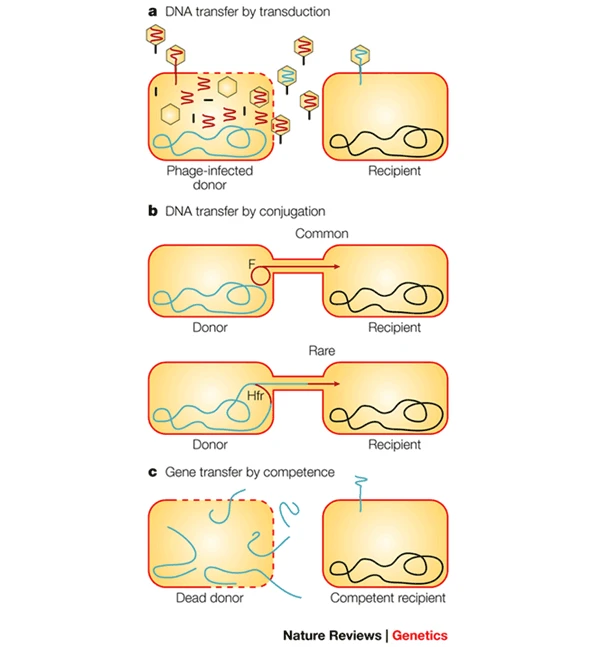
\includegraphics[width=0.8\columnwidth]{Chapter0/Figs/methods-of-dna-transfer.png}
\caption{{An illustration of the three main mechanisms of horizontal inheritance in bacteria. \textbf{a}) Transduction is facilitated by phages that encapsulate host DNA in one cell and eject that DNA into another cell. \textbf{b}) Conjugation, in its prevalent form, is the transfer of a plasmid copy from a donor to a receiver cell via a pilus "bridge". In a rarer form, a plasmid that has been incorporated into the donor cell chromosome is transferred. \textbf{c}) Transformation (competence) is the uptake of exogenous DNA and subsequent incorporation into the chromosome.}
{\label{fig:horizontal-inheritance}}
}
\source{Reprinted by permission from Springer Nature Customer Service Centre GmbH: Springer Nature \textit{Nature Reviews Genetics} \cite{Redfield2001}, Copyright © Nature Publishing Group (2001)}
\end{center}
\end{figure}

\noindent
These different means of inheritance compound to create varying diversity levels within bacterial species and give rise to the \emph{pan-genome}.

\subsection{The pan-genome}

A pan-genome is the full complement of genetic loci found within a given species. Traditionally, loci refer to genes, although we note that loci need not be genes for the work we will describe in this thesis.

The pan-genome can be broken into two subsets: the \emph{core} and \emph{accessory} genome. Loci that occur in the majority of species members are considered core, whilst everything else is deemed accessory (see \autoref{fig:pangenome-venn}). The accessory genome can be further divided into intermediate and rare loci. 

The proportional size of the core genome varies dramatically between species. For instance, if we assume a gene is core when present in $\ge 95$\% of sampled species, the \textit{Escherichia coli} pan-genome is composed of 10\% core genes. Conversely, 89\% of the \textit{Mycobacterium tuberculosis} pan-genome is core genes (data was obtained from the panX database \cite{panx}). Species with a large pan-genome, such as \ecoli{}, have what is called an "open" pan-genome, while those with more conserved gene content, such as \mtb{}, are deemed "closed". 

Another interesting property of the bacterial genome is the distinctive "U-shaped" gene frequency distribution \cite{Lobkovsky2013,pandora,Lapierre2009}, shown in \autoref{fig:pangenome-freq}. This frequency distribution is a consequence of the fact that, in general, genes are either rare or common due to selective pressures \cite{Lobkovsky2013,thepangenome2020}. Moreover, the size of the bacterial pan-genome is estimated to be infinite \cite{Lapierre2009}, as hinted at by \autoref{fig:pangenome-size}.

\begin{figure}
     \centering
     \begin{subfigure}[b]{0.475\textwidth}
        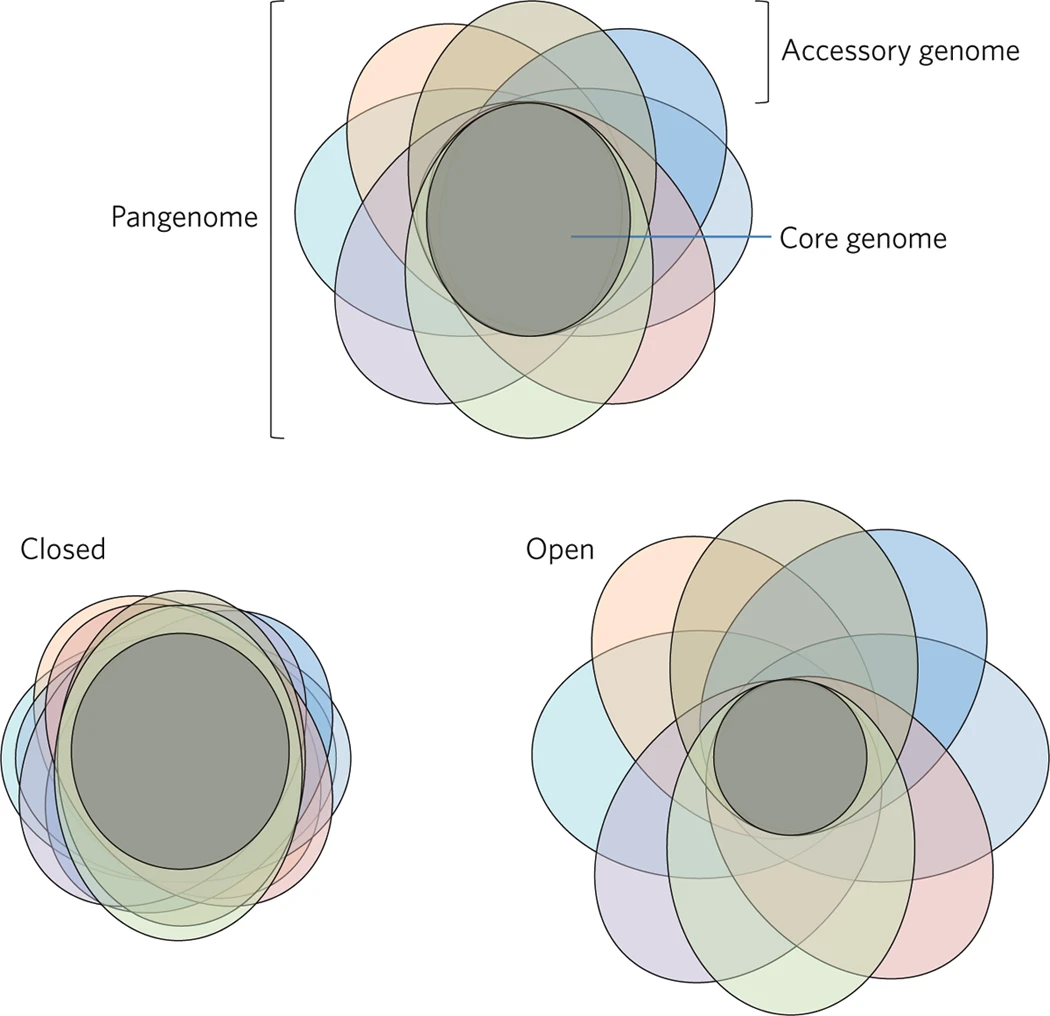
\includegraphics[height=0.21\textheight]{Chapter0/Figs/pangenome-venn.png}
        \centering
        \caption{}
        \label{fig:pangenome-venn}
        \source{Reprinted by permission from Springer Nature Customer Service Centre GmbH: Springer Nature Nature Microbiology \cite{McInerney2017}, Copyright © 2017, Macmillan Publishers Limited.}
     \end{subfigure}
     \begin{subfigure}[b]{0.475\textwidth}
         \centering
        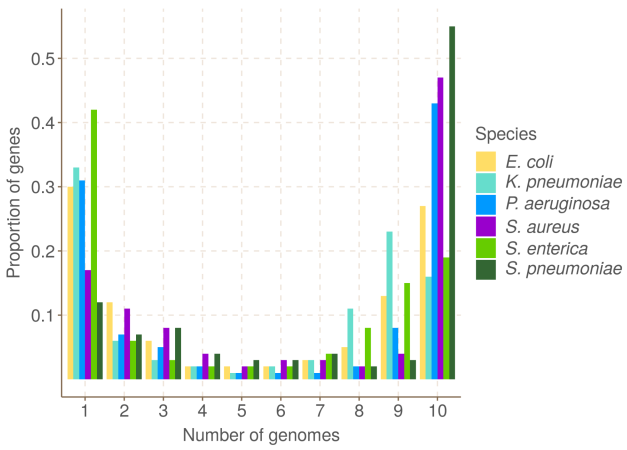
\includegraphics[height=0.21\textheight]{Chapter0/Figs/gene_frequency_distribution.png}
         \caption{}
         \label{fig:pangenome-freq}
         \source{\cite{pandora} under the terms of the \href{https://creativecommons.org/licenses/}{Creative Commons CC BY license}}
     \end{subfigure}
     \begin{subfigure}[b]{0.8\textwidth}
        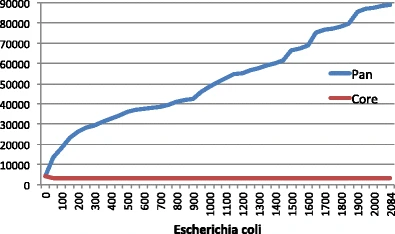
\includegraphics[width=1\linewidth]{Chapter0/Figs/pangenome-size.png}
        \centering
        \caption{}
        \label{fig:pangenome-size}
        \source{\cite{Land2015} under the terms of the \href{https://creativecommons.org/licenses/}{Creative Commons CC BY license}}
     \end{subfigure}
    \caption{The size and gene frequency distribution of the bacterial pan-genome. \textbf{a}) Venn diagram representation of the pan-genome and its core and accessory components. \textbf{b}) The asymmetric U-shaped gene frequency distribution for 10 genomes within 6 bacterial species. Genes are generally rare (left) or common (right). \textbf{c}) the size (y-axis) of the core (red) and accessory (blue; Pan) genome of \ecoli{} as more genomes are sampled (x-axis).}
        \label{fig:pangenome}
\end{figure}

\noindent
These definitions of the pan-genome components (core and accessory) are somewhat simplistic. Recent work by Horesh \etal{} has highlighted that these traditional definitions are biased by lineage sampling \cite{Horesh2021}. For example, we have a collection of 100 genomes, with 50 being from the same lineage ($L_1$). Let us say gene \textit{abc} occurs in all 50 members of $L_1$, but none of the other 50 genomes. Under the traditional pan-genomic definitions, we would call \textit{abc} an intermediate accessory gene. However, if we gathered a further 1,000 genomes, none of which are lineage $L_1$, \textit{abc} would now be considered rare. In the new pan-genome model proposed by Horesh \etal{}, loci are given a classification that is structure-aware. The \textit{abc} gene from our example would be classified as "lineage-specific core", acknowledging the fact that the sampled lineages in a collection provide essential contextual information. Other categories include multi-lineage and collection core and the same categories for intermediate, rare, and a new varied frequency class. The collection core is analogous to the traditional core, with everything else being the accessory genome - albeit with a much finer level of detail.

\subsection{How are pan-genomes analysed?}
\label{sec:analyse-pangenome}

Most pan-genomic analyses of bacterial collections follow a similar approach: align the genomes with a tool such as Parsnp \cite{Treangen2014} or Rory \cite{Page2015}, extract the core genome alignments and either ignore the accessory genome or produce a presence-absence matrix of it \cite{Arnold2018,Azarian2018,McNally2016,thepangenome2020}. When the accessory genome is investigated at the nucleotide level, it is generally focused on a small subset of genes related to specific phenotypes such as antimicrobial resistance (AMR; \cite{Boolchandani2019}) or virulence \cite{Vasquez2019}. However, as we have seen, the pan-genome size varies significantly, so depending on the species, such approaches could be "ignoring" large portions of the total genomic repertoire. Despite this, we have learned an enormous amount about bacteria and their pan-genomes with these methods.

\subsection{Variant calling of bacterial genomes}
\label{sec:intro-bacteria-var-call}

A typical (pan-)genomic analysis requirement, and a focus of this thesis, is variant calling. However, depending on the application, this can be done in many different ways. For example, when characterising an outbreak, common approaches are to use a reference genome of the same, or very close, strain to the outbreak \cite{Taylor2015}, or assemble each sample and select the closest reference to it based on some typing strategy \cite{Wyres2021}. Alternatively, a reference-free approach can alleviate some of the reference bias induced when selecting a genome to call variants against and provide better resolution of an outbreak \cite{Cremers2020}.

Given the importance of bacterial variant calling to this thesis, we will briefly outline various approaches to calling variants in bacterial genomes and highlight their strengths and limitations.

\subsubsection{Alignment-based methods}
\label{sec:aln-var-call}
Alignment-based variant calling requires a reference genome. In this mode of variant calling, raw sequencing reads are aligned to a given reference genome to generate a Sequence Alignment/Map (SAM) file. Common software programs used to perform these alignments for bacterial variant calling include BWA-MEM \cite{li2013}, Bowtie2 \cite{bowtie2012}, and Novoalign (\url{http://www.novocraft.com/products/novoalign}) for short (Illumina) read technology. (\ont{}-based variant calling will be detailed in \autoref{sec:ont-var-calling-intro}, for now we focus on Illumina-based sequencing reads). 

Where variant calling programs distinguish themselves is in how they handle the alignment information. This includes, but is not limited to, the number of base calls disagreeing with the reference, the quality of the read alignment, the alignment locations of a read pair, or the quality score of the mapping \cite{Olson2015}. Popular methods for calling variants generally employ either Bayesian, likelihood, or machine learning algorithms to infer candidate variants given this alignment data. While many of these models were designed for human variant calling, a selection have shown themselves to be perfectly applicable to bacteria. The most frequently used Bayesian method for bacterial variant calling is Freebayes \cite{Garrison2012}; however, it is generally used via a wrapper, Snippy (\url{https://github.com/tseemann/snippy}), which handles the alignment (BWA-MEM), variant calling (Freebayes), and additionally applies filters to the resulting VCF file. Of the likelihood-based callers, Samtools/BCFtools \cite{bcftools2021,samtools2009} and GATK \cite{Poplin2018} tend to be most often employed. 

\subsubsection{Alignment-free methods}
In general, methods that do not align reads to a reference genome use \kmer{}-based algorithms for variant inference. FastGT \cite{fastgt2017} and LAVA \cite{lava2016} are two such programs that require a database of known variants and use \kmer{} counts in a sample to determine the presence of any of these variants. The major limitation with these tools is their inability to call variants not present in the provided database. Kestrel \cite{kestrel2017} is a \kmer{}-based variant caller that can \denovo{} discover variants and does this by detecting unique \kmer{}s in a sample, with respect to a given reference genome. However, Kestrel is not strictly alignment-free, as it does use local alignment to place candidate variants in relation to the reference genome. Additionally, it was shown to have much lower sensitivity than alignment-based methods. 

Another popular alignment-free single nucleotide polymorphism (SNP) caller is kSNP, which finds SNPs \emph{between} samples by detecting \kmer{}s where the central base varies \cite{ksnp2015}. It is regularly used in outbreak settings where differences between samples are crucial \cite{Bazan2017,Raphael2016,Chochua2017}. However, kSNP cannot detect SNPs within $k$ positions (bases) of each other or detect indels, and cannot deal with sequencing errors - requiring extensive pre-filtering.

A benchmark of alignment-free methods for various sequence analysis applications can be found in \cite{Zielezinski2019}. 

\subsubsection{Assembly-based methods}
\label{sec:asm-var-call}
There are two forms of assembly-based variant calling. In the first, an assembled genome for a sample (or samples) is compared to a reference via whole-genome alignment. Software such as MUMmer \cite{mummer2018} or Minimap2/paftools \cite{li2018} facilitate this assembly-to-assembly alignment and then identify positions where the two disagree. An assembly-based method that is prevalent in bacterial genomics is Parsnp \cite{Treangen2014}, which aligns the \emph{core} genome of assemblies and then calls SNPs (only) \emph{between} those genomes. A major limitation with these types of assembly-based approaches is that there is no sense of the quality of calls. As an assembly naturally has a depth of 1x at all positions, there is no information about variant support - all variants are considered equal in this scheme.

The second form of assembly-based variant calling performs assembly and genotyping. Cortex \denovo{} assembles a sample from sequencing reads and genotypes variants at "bubble" sites in its de Bruijn graph \cite{iqbal2012}. It produces variant calls with respect to a provided reference genome and has been used extensively in bacterial genomics \cite{bradley2015,hunt2019,Stasiewicz2015,Young2017,Lees2017}.

\hspace{0.75cm}

\noindent
A recent comprehensive benchmark of alignment-based variant calling found that the choice of reference genome, rather than the choice of tools, has the most critical impact on accuracy \cite{Bush2020}. The best general-purpose pipeline was found to be Snippy; however, they note that species-specific filtering of the final VCF file can cause the performance of many tools to converge.

Reference genome bias is the most significant limitation of bacterial variant calling approaches \cite{Bertels2014,Bush2020,Olson2015}. The bacterial pan-genome highlights this impediment in a stark way. As an illustration of this, \autoref{fig:reference-bias} shows a cartoon depiction of the "single-reference problem". In this figure, we see that no two genomes contain the same complete set of loci - precisely what we expect from nearly any pan-genome \cite{McInerney2017}. Thus, using any of these genomes as a reference to call variants against will inevitably mean we cannot describe variants in loci not found in both the reference and query genomes. This type of bias is termed \emph{hard} reference bias. Another, more subtle, form is \emph{soft} reference bias, which results from difficulties aligning to the reference due to divergence in shared loci between the reference and query - especially around structural variants \cite{Price2017,Olson2015,Pightling2014}. However, these biases tend to impact clonal species, such as \mtb{}, much less than those with open pan-genomes \cite{Bush2020}.

\begin{figure}
\centering
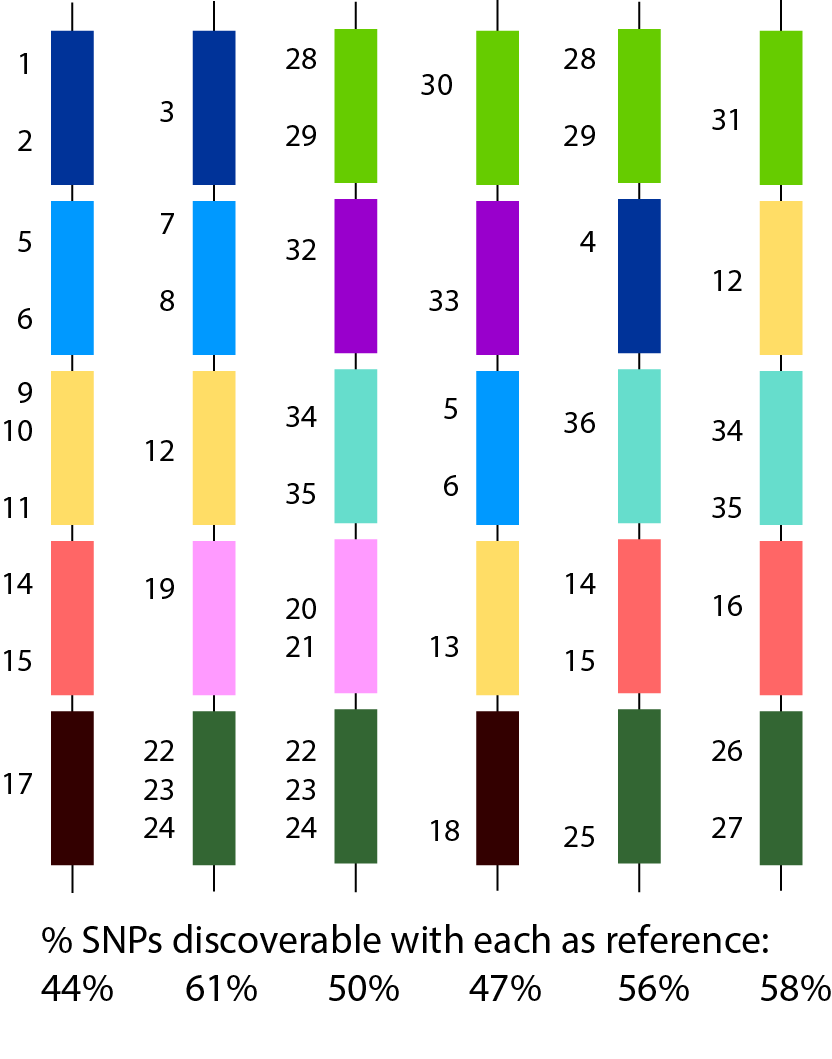
\includegraphics[height=0.35\textheight]{Chapter0/Figs/single_ref_problem.png}
\caption{An illustration of the single-reference problem. Each vertical column depicts a genome, with the coloured blocks representing loci (genes). The numbers next to each locus indicate a variant with respect to other loci of the same colour. The percentage figures at the bottom indicate what percentage of variants in the other genomes could be found by a perfect variant caller if that genome was used as a reference. Not all genomes contain the same loci; hence no genome can capture all of the variants.}
\label{fig:reference-bias}
\source{\cite{pandora} under the terms of the \href{https://creativecommons.org/licenses/}{Creative Commons CC BY license}}
\end{figure}

Given the biases resulting from the use of a single reference genome, an alternative solution is needed. One solution that is rapidly maturing is the use of a \emph{genome graph} to replace a single reference.

% =============================================
\section{Genome graphs}

Genome graphs are a way of representing variation within a population, be it a bacterial species, a human gene, or a viral quasi-species \cite{comp-pan-genomics}. \autoref{fig:graph-representation} illustrates a generic representation of a genome graph, where redundant information (consensus) is collapsed into a linear sequence and variation is represented as divergent paths leading in and out of these consensus segments. Thus, a walk (path) through such a graph represents a mosaic of the population variation. 

A rich array of algorithms and methods have been proposed for representing and operating on genome graphs across all kingdoms of life \cite{Sherman2020,Eizenga2020,comp-pan-genomics}. In this section, we will highlight some mature genome graph frameworks, along with their limitations. In the context of this thesis, limitations will focus on the applicability of a method to the bacterial pan-genome. Finally, we follow these existing methods by introducing a new genome graph approach relevant to this thesis.

\begin{figure}
\centering
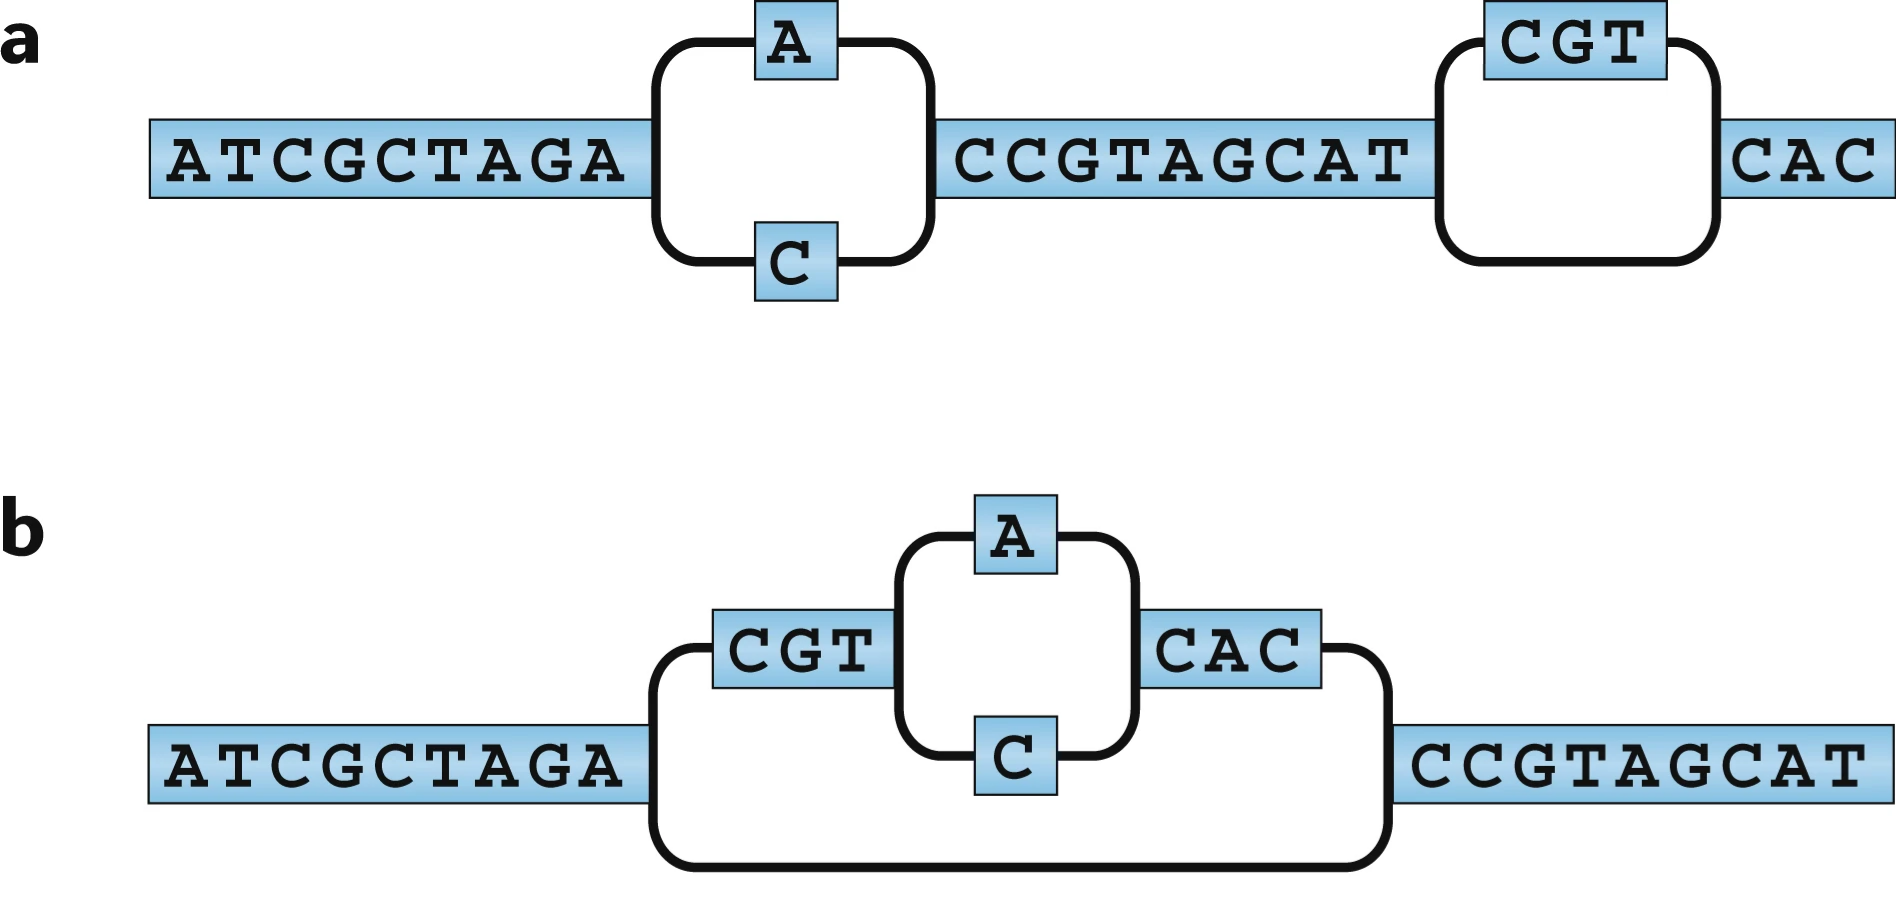
\includegraphics[width=0.6\columnwidth]{Chapter0/Figs/graph-representation.png}
\caption{Conceptual representation of a genome graph. \textbf{a}) Variants cause a "bubble", or divergent path. Note, the second bubble represents an insertion/deletion. \textbf{b}) Variation can be arbitrarily nested. In this example, there is a SNP within an insertion. \textbf{c}) Haplotype information can be encoded by "colouring" variants and disallowing paths that mix colours.}
\label{fig:graph-representation}
\source{Reprinted by permission from Springer Nature Customer Service Centre GmbH: Springer Nature Nature Reviews Genetics \cite{Sherman2020}, Copyright © 2020, Springer Nature Limited.}
\end{figure}

\subsection{Existing methods}
\label{sec:graphs-existing}

\subsubsection{GraphTyper}
GraphTyper \cite{graphtyper,graphtyper2} represents a genome graph as a directed acyclic graph (DAG) built from a reference sequence plus known variants (similar to \autoref{fig:graph-representation}, but with directionality). Sequencing reads are mapped to the reference genome with BWA-MEM. The reference sequence is then broken into 50kbp regions, and reads are realigned to the graph in the respective region they map to. A path for the read is detected using a seed-and-extend approach, and variants are genotyped based on the read-support from this alignment. Impressively, GraphTyper can genotype SNPs, indels, and complex and structural variants.

In the context of bacterial genomes, there are several limitations with GraphTyper. First, a single reference genome is used as the backbone of the graph. This is a feasible solution for humans, but not for bacteria, where, as we have seen, it is likely that two genomes do not have an identical gene repertoire. Second, the initial alignment of reads to the reference genome suffers the same soft and hard reference bias discussed in \autoref{sec:intro-bacteria-var-call}. The realignment of reads reduces the soft reference bias compared to linear genome methods; however, the hard bias remains. Third, no long-read sequencing technology support is available and is unlikely to be possible with the current seed-and-extend approach used for alignment \cite{li2018}. 

\subsubsection{Variation graph toolkit}
The Variation Graph Toolkit (VG) \cite{vg2018} is a suite of tools for construction, alignment, and genotyping of genome graphs. The representation used by VG is an \emph{un}directed, potentially cyclic, graph. Variation graphs can be constructed from a single reference and associated VCF file or multiple genome assemblies. Read alignment to the graph uses a seed-and-extend approach. Variant calls are made via a basic read pileup on the graph and then augmenting the original graph with novel candidates, followed by genotyping \cite{Novak2017}.

As with GraphTyper, the use of seed-and-extend alignment makes the support of long reads unlikely. (We note there have been discussions within the VG GitHub repository for four years about supporting long reads; however, no support has been announced). Another limitation of VG is that in order to produce variant calls, the user must provide a reference genome, again, either inheriting reference bias or requiring a verbose description of simple variants (see \autoref{sec:pandora-compare} for an elaboration of this point).

A significant limitation of VG is its computational resource requirements. As VG attempts to be a "general" method - i.e., it is undirected and allows cycles to support events such as inversions and repeats naturally - it is CPU and disk intensive \cite{strainflair2021,gramtools2021,minigraph2020} to the point of requiring over one terabyte of temporary disk space to construct a graph \cite{gramtools2021}, or not being useable \cite{minigraph2020}.

\subsubsection{Minigraph}
Minigraph \cite{minigraph2020} represents a genome graph as a bidirectional graph, which allows cycles. The construction process starts with a single genome and iteratively adds structural variants (SVs; regions of divergence $\ge 100$bp and $\le 100$kbp). In each round, a genome is aligned to the existing graph (a linear sequence in the beginning), augmenting it with sequence from poorly mapped regions (SVs). Minigraph aligns sequencing reads or assemblies to this graph using a modified version of minimap2's minimizer \kmer{}-based seed-and-chain approach \cite{li2018}. As such, Minigraph should inherently support long reads.

As Minigraph only incorporates SVs of 100bp or longer, it does not variant-call in the typical sense. It instead produces a BED-like file that calls SVs from the alignment. This is the main limitation of Minigraph: it cannot call variants smaller than 100bp, which are especially important in bacterial genomes. However, the authors acknowledge this limitation and state that the reason for this exclusion is that smaller variants can be easily identified with standard approaches. 

\subsubsection{Gramtools}
Gramtools \cite{gramtools2016,gramtools2021} represents a genome graph as a DAG that can be constructed from either a single reference and associated VCF file or a multiple sequence alignment (MSA) (it uses the same model outlined below in \autoref{sec:make_prg}). Alignment of sequencing reads is facilitated by the variation-aware Burrows-Wheeler Transform (vBWT; \cite{gramtools2016}), which is an extension of the original linear BWT to graphs. It genotypes variants under a haploid or diploid likelihood-based model and produces variant calls in the standard VCF. Alternatively, Gramtools can write variant calls to a new JSON-like VCF (jVCF) file, which stores the standard VCF information, with the addition of graph-relevant details about the nesting of sites \cite{gramtools2021}. As with the other genome graph methods, though, Gramtools only supports short Illumina sequencing data and is unlikely to support long reads with a higher error rate than Illumina.

\noindent
All existing genome graph methods require an enforced ordering - i.e., loci are not considered independently. Despite the fluidity of bacterial genomes, there is surprisingly conserved gene ordering \cite{Tamames2001,Rocha2008}. However, the enforced order of these genome graphs cannot account for variations in gene repertoire - i.e., the bacterial pan-genome. 

VG has been applied to bacteria for strain-typing and abundance estimates in \ecoli{}; however, individual graphs need to be concatenated together for each gene, thus enforcing an order \cite{strainflair2021}. None of the methods, to our knowledge, natively allows the independence of loci. This behaviour can be approximated but requires custom pipelines, as in \cite{strainflair2021}. Additionally, no existing genome graph method supports long-read sequencing technologies such as \ont{}.

These limitations are a driving motive for the development of the genome graph method Pandora.

\section{Pandora: bacterial pan-genomics with reference graphs}
\label{sec:pandora-intro}

As we have seen, the bacterial pan-genome can be amazingly diverse at both the nucleotide and gene (locus) levels. Thus, using a single reference to describe such variation is inadequate; the pan-genome seems a perfect application for genome graphs. However, existing methods fail to allow for structural differences at the locus level (\autoref{sec:graphs-existing}) and therefore are unable to describe nucleotide-level variation in the accessory genome. Another shared limitation of existing genome graph tools is the lack of support for long-read sequencing technologies (we outline the significance of this in \autoref{sec:intro-ont}).

Pandora is a genome graph method that addresses these limitations. Rachel Colquhoun developed \pandora{} during her PhD thesis \cite{rachelthesis}; we provide a brief overview of its methodology here as we extend and apply it throughout this thesis.

\subsection{Population reference graph construction}
\label{sec:make_prg}

The genome graph representation used by \pandora{} is a DAG. However, unlike Gramtools, which uses the same representation \cite{gramtools2021}, \pandora{} is agnostic to locus ordering. Instead, \pandora{} interprets a genome graph (interchangeably referred to as a \emph{reference graph}) at two levels: locus and pan-genome. We call a locus-level reference graph a \emph{population reference graph} (\prg{}) as it represents the variation within a given population for a locus. A \prg{} is not restricted in its scope for a locus; it can be a gene, intergenic region, operon, or any other grouping desired. A pan-genome-level reference graph is termed a \emph{pan-genome reference graph} (\panrg{}) and is a collection of \prg{}s. Again, a \panrg{} is not limited in its scope; it could describe a pan-genome, a meta-genome, or a collection of antimicrobial resistance-associated genes.

Construction of a \prg{} is accomplished with a recursive cluster and collapse algorithm, implemented in the software program \makeprg{} (\url{https://github.com/iqbal-lab-org/make_prg}; \cite{rachelthesis,pandora}). Two parameters are key to this process: the minimum match length, $m$, and the maximum nesting level, $n$. Starting with an MSA of locus sequences, when $\ge m$ positions agree, they are collapsed into a single sequence. The remaining non-collapsed sections of the MSA are recursively clustered, with (sub)sequences in the cluster being collapsed or clustered again. This recursive clustering and collapsing continues until all clusters contain a single sequence or recursion has occurred more than $n$ times. This process is illustrated in \autoref{fig:make-prg-rcc}, which uses $m=4$ and $n\ge 2$.

\begin{figure}
\centering

\includegraphics[width=1\columnwidth]{Chapter0/Figs/make-prg.png}
\caption{Construction of a locus reference graph (\prg{}) from a multiple sequence alignment (MSA; left) with the recursive cluster and collapse algorithm implemented in \makeprg{}. Vertical slices in the MSA are collapsed when there is a minimum match length of 4. Sections not collapsed are recursively clustered and collapsed (if possible), until no further clustering is possible or a maximum nesting level is attained. In this example, a nesting level of 2 is reached.}
\label{fig:make-prg-rcc}
\source{\cite{pandora} under the terms of the \href{https://creativecommons.org/licenses/}{Creative Commons CC BY license}}
\end{figure}

\subsection{Index, quasi-map, and sequence inference}

\subsubsection{$(w,k)$-minimizers}
A core concept within \pandora{} is $(w,k)$-minimizers \cite{Roberts2004} - interchangeably referred to as minimizer (or minimizing) \kmer{}s. A $(w,k)$-minimizer is a representative \kmer{} from a collection of $w$ consecutive \kmer{}s in a string (sequence). The function used to select this representative can use any ordering one prefers; \pandora{} uses the same ordering strategy as minimap \cite{minimap2016} - the \kmer{} with the minimum invertible integer hash function value. The purpose of minimizer \kmer{}s is to reduce the number of \kmer{}s required to represent a sequence but ensure that if two strings share a significant exact match, they will share at least one minimizer. Additionally, \pandora{} requires $w\le k$, ensuring all \prg{} bases are covered by a minimizer (except, at most, the first and last $w-1$ bases).

\subsubsection{Indexing}
Each \prg{} is represented within \pandora{} as a minimizer \kmer{} graph. This graph is constructed by walking all paths in the \prg{} and selecting minimizer \kmer{}s as outlined above. As $w\le k$, walking each path ensures a minimizer covers every site within the graph. The index of a \panrg{} is a map from a minimizer \kmer{} to the position(s) and \prg{}(s) it occurs in. 

\subsubsection{Quasi-mapping}
\label{sec:quasi-map}
Quasi-mapping - as opposed to mapping - is a form of approximate alignment. The goal of quasi-mapping is to identify which locus (or loci) a read originates from, and \emph{roughly} where within that locus each section of the read maps. To perform this quasi-mapping, \pandora{} looks up all $(w,k)$-minimizers of a read in the index. Then, for every read minimizer that occurs in the index, a \emph{hit} (read and \prg{} positions) is recorded. A single read minimizer can have multiple hits if the minimizing \kmer{} occurs in multiple locations in the \panrg{}. As such, once all hits are identified, they are filtered to remove spurious ones. This filtering is done by keeping only those hits that cluster together on a read and only occur in a single \prg{}. Thus, all \prg{}s associated with a cluster of hits are deemed present in the sample, while the remaining loci are considered absent.

\subsubsection{Sequence inference}
\label{sec:seq-inference}
A major reason for \pandora{}'s reduced reference bias is that it does not demand a single reference genome. Instead, it takes a \panrg{} and infers the closest sequence in that \panrg{} to the sample under consideration. As we saw in \autoref{sec:intro-bacteria-var-call}, the choice of reference is often the biggest limitation when calling variants in bacterial genomes.

For each \prg{} deemed present after quasi-mapping, \pandora{} has (filtered) coverage information for the minimizers in the \kmer{} graph. A dynamic programming algorithm is used to find the path through the \kmer{} graph that maximises the log-likelihood score. This inferred sequence (path) is also referred to as the \emph{maximum likelihood path}.

\subsection{Variation inference}

\subsubsection{Single-sample}
The single-sample inference and genotyping mode of \pandora{} is coordinated by the \map{} routine. It quasi-maps sequencing reads to the \panrg{} and infers a sequence for each \prg{}. In addition, if requested, \map{} will also genotype the sample against the maximum likelihood path for each \prg{} (or a user-provided sequence if it exists). Thus, genotyping occurs for all variation sites within the \prg{} and is returned as a VCF file. An example of this single-sample genotyping and VCF is shown in \autoref{fig:map-var-representation}.

\subsubsection{Multi-sample}
\label{sec:pandora-compare}
Variation inference can also be performed for a collection of samples with the \compare{} protocol. Reference bias problems have traditionally plagued this type of analysis. If the collection of samples are of the same strain, then analysis against the same reference is not problematic, but once even a single sample originates from a different strain, the pan-genome exerts itself. As we outlined in \autoref{sec:analyse-pangenome}, analysing divergent samples generally works by looking at variation in the core genome while resorting to locus presence-absence in the accessory genome. Multi-sample inference with \compare{} offers the best of both worlds; variation is inferred for both the core and accessory genome. Where a locus is absent from a sample, all sites for that locus are represented with a null genotype. In this approach, if a locus is present in only 2/20 samples in the collection, variants for that locus are only inferred for those two samples.

To allow this multi-sample variation inference, \pandora{} infers the maximum likelihood path for each sample (\autoref{sec:seq-inference}). Then, using the same dynamic programming algorithm, \pandora{} infers a maximum likelihood path for \emph{the collection} of samples; instead of \kmer{} coverage, the number of maximum likelihood paths covering each minimizer is used for inferring the most likely path. In the end, the inferred sequence is selected to be maximally close to all samples in the collection. Therefore, all samples are genotyped against the same reference at all variant sites, making direct sample comparisons possible. This approach also ensures that small differences between samples are described as such - as shown in \autoref{fig:var-representation}.

\begin{figure}
     \centering
     \begin{subfigure}[b]{0.95\textwidth}
        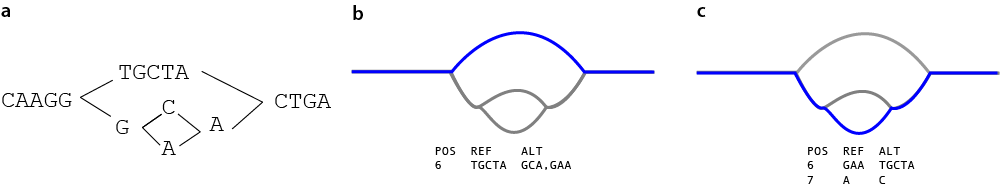
\includegraphics[width=0.95\columnwidth]{Chapter0/Figs/map_variation_representation.png}
        \centering
        \caption{Single-sample variation inference}
        \label{fig:map-var-representation}
        \source{\cite{rachelthesis}}
     \end{subfigure}
     \begin{subfigure}[b]{0.95\textwidth}
         \centering
        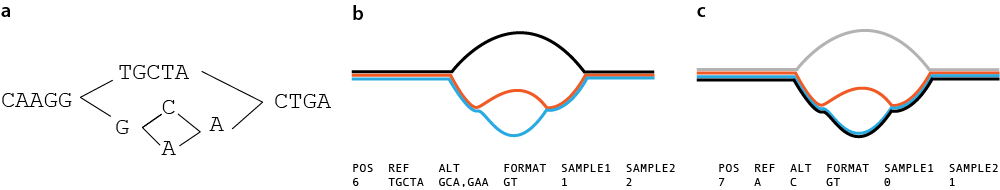
\includegraphics[width=0.95\columnwidth]{Chapter0/Figs/variant_representation.png}
         \caption{Multi-sample variation inference}
         \label{fig:var-representation}
         \source{\cite{pandora} under the terms of the \href{https://creativecommons.org/licenses/}{Creative Commons CC BY license}}
     \end{subfigure}
     \caption{The impact of sequence inference on variant representation. In both \textbf{(a)} and \textbf{(b)} the left panel (i) shows the \prg{}. \textbf{a)} the blue line indicates the inferred sequence (maximum likelihood path). ii and iii show how the choice of this sequence affects the representation of variant sites when genotyping. \textbf{b}) the black line indicates the multi-sample inferred sequence, while the blue and orange lines are two different samples. ii and iii show that small differences between the samples are represented as small variants by inferring the sequence that is maximally close to the two samples (iii).}
     \label{fig:pandora-var-representation}
\end{figure}

\hspace{0.75cm}

\noindent
The \pandora{} method addresses the main limitations of existing genome graph approaches (\autoref{sec:graphs-existing}) in the context of bacterial pan-genomes. In particular, \pandora{} supports both short (Illumina) and long (\ont{}) sequencing reads and removes hard reference bias by letting go of locus ordering and genotyping loci regardless of their genomic context.

Despite these advantages, the method has a notable limitation: an inability to detect novel variants. As variation inference is achieved by genotyping all sites in a \prg{}, it follows that if a variant does not exist in a \prg{}, it cannot be detected by \pandora{}. \autoref{chap:denovo} of this thesis will address this limitation. 

% =============================================
\section{\ont{} sequencing}
\label{sec:intro-ont}
The sequencing of DNA and RNA with a nanopore was conceived of by multiple parties in the 1980s \cite{Deamer2016}. However, it was not commercially available until the release of the Oxford Nanopore Technologies (ONT) MinION\textsuperscript{\texttrademark} device in 2014 \cite{Quick2014,Deamer2016}. (We use \emph{\ont{}} sequencing to indicate sequencing with an ONT device throughout this thesis). The MinION device is smaller than a smartphone and plugs into a computer's USB port.

\ont{} sequencing works by passing a strand of DNA or RNA through a nanopore. The nanopore is embedded in an electro-resistant membrane, with a flow cell containing an array of such pores. A sensor attached to each nanopore records the electrical current passing through it; as the DNA or RNA strand moves through the nanopore, this current signal changes. There are approximately five nucleotides present in the nanopore at a time. As such, the identity of each nucleotide (base) can be inferred by a characteristic signal alteration (see \autoref{fig:nanopore}). Because the sensor takes measurements at a faster speed than the DNA moves through the nanopore, multiple recordings are obtained for each base transition - see the distinctive "steps" in \autoref{fig:nanopore}b. The process of inferring a DNA or RNA sequence from this raw signal is called \emph{basecalling}.

\begin{figure}
\centering
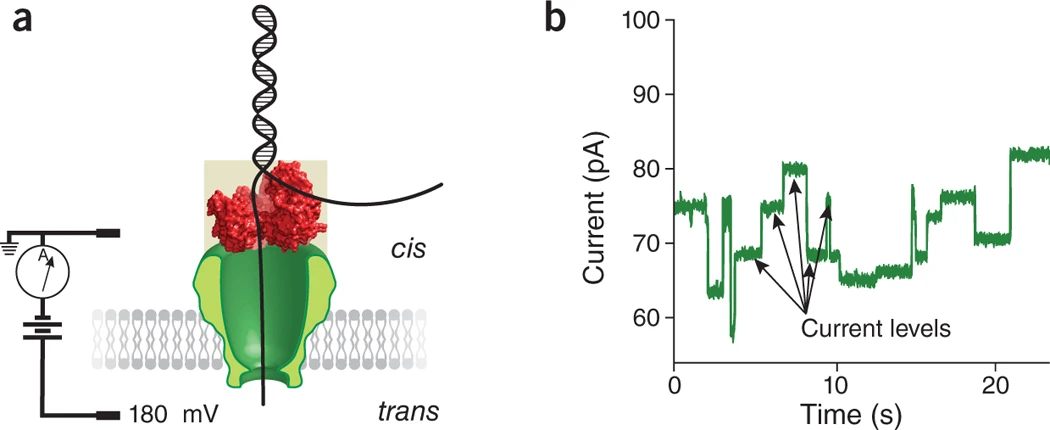
\includegraphics[width=0.9\columnwidth]{Chapter0/Figs/nanopore.png}
\caption{Nanopore sequencing. \textbf{a}) A single strand of DNA or RNA (black) is passed through a nanopore (green) by an enzyme (red). A sensor records the electrical current flowing through the nanopore. \textbf{b}) The raw signal (electrical current; y-axis) changes as nucleotides move through the nanopore. Each nucleotide can be inferred by a characteristic alteration in the signal, indicated by the black arrows.}
\label{fig:nanopore}
\source{Reprinted by permission from Springer Nature Customer Service Centre GmbH: Springer Nature Nature Biotechnology \cite{Deamer2016}, Copyright © 2016, Nature Publishing Group.}
\end{figure}

\subsection{Basecalling}

The raw signal and metadata for each molecule read by a nanopore are deposited into a hierarchical data format file (HDF5; referred to as a \emph{fast5} file; \cite{hdf5}). Furthermore, these fast5 files are produced in real-time. Thus, the user has immediate access to the sequencing data as soon as it is produced, a unique advantage over existing sequencing technologies.

Basecalling algorithms have seen substantial development since the release of ONT's first device. The progression of these algorithms, along with nanopore structure and chemistry, has led to a steady increase in the accuracy of genomic sequences inferred from \ont{} sequencing (as shown in \autoref{fig:nanopore-timeline}; \cite{Rang2018}). For example, from an initial read-level accuracy of approximately 60\% \cite{Goodwin2015}, recent studies have reported accuracy of 93.2\% \cite{Silvestre2021}.

Traditionally, there were two key components to basecalling. The first was the segmentation of the raw signal into "events" (the plateaus in \autoref{fig:nanopore}). These events represent a 5-mer within the nanopore; therefore, consecutive events describe a sequence of nucleotides entering and leaving the nanopore. The second component of traditional basecalling is applying an algorithm to these events to infer the genomic sequence. 

Basecalling algorithms require an \textit{a priori} model trained on molecules for which the sequence is known. Metrichor was the original software provided by ONT for basecalling; it used a hidden Markov model (HMM) to turn events into a sequence. In 2017, Boža \etal{} developed the first basecalling method to use a recurrent neural network (RNN) - instead of an HMM - to turn events into sequence with increased accuracy \cite{deepnano}. RNN basecalling was provided soon after this with ONT's new Albacore algorithm. The following major algorithmic development was the removal of the segmentation step (the most error-prone stage of basecalling). These programs, Chiron and BasecRAWller, used a Connectionist temporal classification (CTC) decoder to label unsegmented raw signal and subsequent basecalling with an RNN and convolutional neural network \cite{chiron2018,Stoiber2017}. Again, soon after this, ONT released a new basecalling program, Guppy, which incorporated these new ideas. Since its release, Guppy has been the gold-standard basecalling algorithm, and all algorithmic development has focused on labelling the raw signal data.

\begin{figure}
\centering
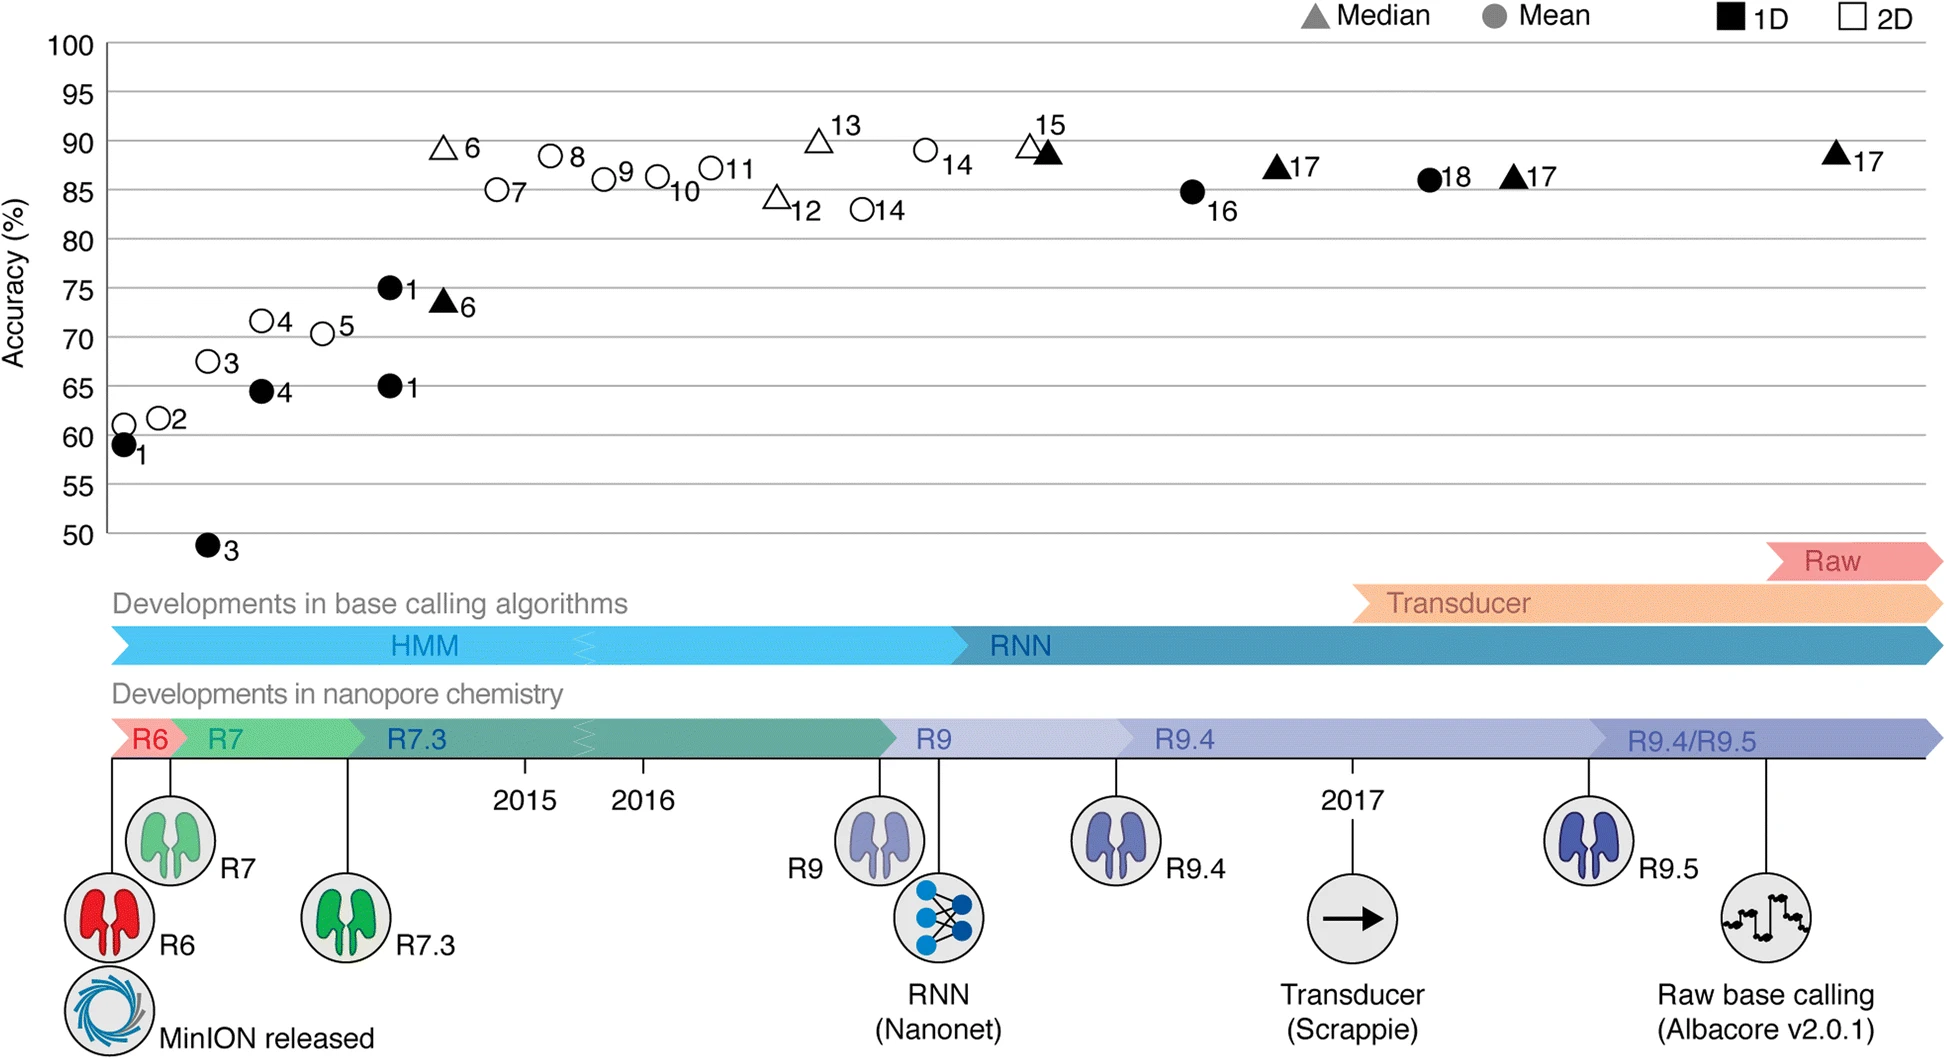
\includegraphics[width=0.9\columnwidth]{Chapter0/Figs/nanopore_timeline.png}
\caption{Timeline of ONT nanopore chemistry and the accuracy of \ont{} sequencing data. The numbers attached to each point in the accuracy plot relate to published work reporting the accuracy measurement. A list of those publications can be found in the original article this figure was taken from \cite{Rang2018}. HMM=hidden Markov model; RNN=recurrent neural network; 2D=a form of \ont{} sequencing where both strands are sequenced.}
\label{fig:nanopore-timeline}
\source{\cite{Rang2018}}
\end{figure}

\noindent
The pre-trained models distributed with \guppy{} aim to be general. That is, they can be used on \ont{} data from any organism. The species these models were trained with is not common knowledge; however, it is fair to assume a variety were used given \guppy{}'s consistent performance across kingdoms and species. In 2019, Wick \etal{} showed that training a taxon-specific (Enterobacteriaceae) basecalling model can provide increased accuracy when used to basecall a sample from that taxon \cite{wick2019}. Their analysis also revealed that - at least in Enterobacteriaceae - Dcm-methylation sites were the primary source of \guppy{} basecalling errors and that the taxon-specific model removes nearly all of the errors of this type. In addition, as has also been described elsewhere \cite{watson2019}, homopolymer deletions were found to be the next most common source of systematic errors and were also reduced with the use of a taxon-specific model.

The current state of \ont{} basecalling suggests that improvements in accuracy will come from three areas: chemistry, basecalling algorithm, and training data improvements. Therefore, in \autoref{chap:tubby} we will look to improve \ont{} accuracy by focusing on the latter of those areas and training a \emph{species}-specific basecalling model.

\subsection{Variant calling}
\label{sec:ont-var-calling-intro}

Variant-calling from \ont{} sequencing data is slowly maturing but is yet to reach the standards set by other sequencing technologies. Much of the problems relate to the lower read accuracy of \ont{} data compared to Illumina and PacBio. A higher error rate means it is harder for genotyping models to distinguish genuine variants from technology-derived errors.

The first method specifically designed to call variation from \ont{} data was Nanopolish \cite{nanopolish2015,nanopolish2017} - developed in 2015. It maps the raw signal for each read to a reference genome and uses an HMM to determine if the reads show support for a variant. However, Nanopolish requires access to the fast5 files in order to call variants. Operating on fast5 files is incredibly IO intensive, and this contributes to observed Nanopolish runtimes in the order of days, and peak memory in the 100's of gigabytes \cite{clairvoyant2019}. More recent variant callers designed to support \ont{} data such as DeepVariant \cite{deepvariant}, Clairvoyante \cite{clairvoyant2019}, and Clair \cite{clair2020} all use multi-layer neural networks and require significant effort on behalf of the user to operate \cite{sanderson2020}. An ONT-developed variant caller (and sequence correction) tool, Medaka (\url{https://github.com/nanoporetech/medaka}), also uses neural networks but is much simpler to use. In addition to these newer, complex methods, some researchers have found that more traditional short-read approaches such as GATK \cite{Poplin2018} can be tuned to work well with \ont{} data \cite{greig2021,bainomugisa2018,Greig2019}.

Despite the wealth of \ont{} basecalling \cite{wick2019} and assembly \cite{wick2020} benchmarking studies, there is relatively few independent variant calling assessments. A recent analysis by Sanderson \etal{} evaluated Clair, Nanopolish, and Medaka for variant calling in \textit{Neisseria gonorrhoeae} \cite{sanderson2020}. However, this study used Illumina as the "truth" and only assessed SNP calls. They found Clair was the best-performing method and could detect 94-98\% of Illumina SNP calls; however, it required training a random forest classifier to achieve this result. In addition, in order to reduce false-positive SNPs from 49-289/genome to 4-19/genome, SNP detection dropped to 76-94\%. Therefore, it remains to be seen what the true precision and recall of \ont{} variant calling is - for both SNPs and indels.

\subsection{Benefits and limitations}
\label{sec:ont-benefits}

As a result of its vastly different approach to sequencing, \ont{} offers many unique benefits over the gold-standard Illumina. However, there are limitations, and \ont{} will unlikely ever be a solution for all problems. We will briefly summarise some of these pros and cons with respect to Illumina in the context of pathogen genomics and its application to real-world settings.

\subsubsection{Cost}
Depending on the context of the application, \ont{} sequencing is both more and less expensive than Illumina sequencing. At a device and peripherals level, a few layers of cost need to be understood. The upfront price of an ONT MinION device is \euro900, while an Illumina MiSeq costs \euro100,000 - 111 times more than the MinION \cite{Tedersoo2021}. The cost per lane/flow cell and library prep is \euro600 and \euro90-130 for the MinION, while for the MiSeq, these two items are \euro2,000 and \euro50-100, respectively. Considering these prices, the cost of generating one billion bases (1gbp) of sequencing data is \euro12 on a MinION device and \euro175 for a MiSeq. However, the caveat here is that, currently, the 1gbp of Illumina data will be of superior quality. Other costs that are harder to quantify are the need for more extended library preparation for Illumina sequencing, which causes additional labour expenses \cite{Tedersoo2021}.

\subsubsection{Portability}
The ONT MinION weighs just 87g and has a volume of 80cm\textsuperscript{3}, while the Illumina MiSeq respective weight and volume are 57.2kg and 202,709cm\textsuperscript{3}. In addition, the MinION can be powered through the USB port of a computer, while the MiSeq requires significantly more power resources \cite{Tedersoo2021}. These two aspects combine to make the MinION extraordinarily portable and the MiSeq completely stationary.

The benefit of the MinION's portability has famously been exhibited during the Zika and Ebola outbreaks, where \ont{} sequencing was used on-the-ground to aid public health investigations \cite{faria2016,Hoenen2016,quick2016}.

\subsubsection{Diagnostics}
Another benefit of \ont{} sequencing is that the data is made available in real-time. A standard MiSeq runtime is approximately 55 hours \cite{Tedersoo2021}, and therefore it takes at least 55 hours to have access to the sequencing information. In contrast, MinION diagnostics can operate as rapidly as the sequencing. Indeed, \ont{} sequencing has been applied to same-day \mtb{} diagnostics, with phylogenetic placement and full drug susceptibility profiles in 12.5 hours \cite{Votintseva2017}. Other real-time diagnostic applications have included detection of surgical device infections \cite{Sanderson2018}, Ebola \cite{Hoenen2016,quick2016} and Zika \cite{faria2016} virus outbreak surveillance, and Enterobacteriaceae strain and drug resistance identification \cite{Cao2016}. Even conventional genomics for bacterial diagnostics stands to gain from the use of \ont{} sequencing. For example, Greig \etal{} from Public Health England found that the better resolution of the Shiga toxin-producing \ecoli{} accessory genome from \ont{} sequencing lead to improved resolution during outbreak investigation \cite{greig2021}.

Another emerging benefit of \ont{} sequencing is the artificial enrichment/depletion of samples \cite{Payne2021,Kovaka2021}. An API (Read Until) facilitates this enrichment within the MinION device, allowing for ejecting (rejecting) molecules from the nanopore. The sequencing data is mapped to a reference database, and rules can be provided that reject a molecule if it originates from a specified reference or once a certain read depth has been reached. One application by Kovaka \etal{} was to deplete bacterial DNA, thus enriching yeast genetic material \cite{Kovaka2021}; however, this could easily be employed in reverse, depleting human DNA and enriching bacterial or viral material in a patient-derived sample.  

\hspace{0.75cm}

\noindent
While there are many benefits to \ont{} sequencing, the accuracy of data provided is still well behind Illumina. However, as we have seen, increased algorithm and method development is helping to reduce the difference. Therefore, a primary focus of this thesis is the improvement of \ont{}-derived sequencing information. In particular, after adding the ability for \pandora{} to discover novel variants, we will turn our attention to genome graph and \ont{} sequencing applications for the pathogen \textit{Mycobacterium tuberculosis}.

% =============================================
\section{Tuberculosis and its causative agent}

Tuberculosis (TB) is an ancient airborne disease that predominantly affects the lungs \cite{Pai2016}; evidence suggests it has been with humans since leaving Africa \cite{Wirth2008,Comas2013}. In 2019, an estimated 1.4 million people died of TB globally, and over 10 million fell ill to the disease; 206,030 of those cases were multi-drug resistant (MDR) \cite{who2020}. The causative agent of TB is principally the bacteria \textit{Mycobacterium tuberculosis}, which has no known reservoir other than humans \cite{Comas2013}. However, other members of the Mycobacterium tuberculosis complex (MTBC), such as \textit{M. africanum}, can also cause TB \cite{Pai2016}. 

TB is a preventable and curable disease; 85\% of patients with active disease can be successfully treated with a 6-month drug treatment that has the added benefit of preventing transmission \cite{who2020}. Furthermore, estimates show that 60 million TB-caused deaths have been avoided since 2000. Despite this, TB remains in the top 10 causes of death worldwide \cite{who2020}. 

In 2015, the World Health Organization (WHO) and United Nations developed the End TB Strategy, which aims - among other goals - for a 95\% reduction in TB deaths by 2035 \cite{endtb2020}. One of the central pillars of the End TB Strategy is "Intensified research and innovation" through the "discovery, development and rapid uptake of new tools, interventions and strategies." Another pillar, which will be a focus of this thesis, is improved patient-centred diagnostics for the "early diagnosis of tuberculosis including universal drug-susceptibility testing, and systematic screening of contacts and high-risk groups."

We highlight these specific focuses of the End TB strategy as they motivate much of the work in this thesis.

\subsection{Epidemiological and phylogenetic diagnostics}
Public health applications for whole-genome sequencing (WGS) of \mtb{} generally focus on three diagnostic use-cases: species/lineage identification, prediction of drug resistance, and clustering of samples for epidemiological purposes \cite{Gordon2021,Meehan2019}.

\subsubsection{Species/lineage identification}
The MTBC is composed of seven species of Mycobacteria with varying growth, host, and pathology characteristics \cite{Homolka2012}. In addition, non-tuberculous mycobacteria (NTM), such as \textit{M. abscessus} and \textit{M. avium}, can cause infections that present similarly to those of the MTBC \cite{Johansen2020}. However, NTMs can have very different drug resistance profiles to MTBC members \cite{Floto2016,Johansen2020}, highlighting the importance of correct species and lineage identification.

Routine species and lineage identification for suspected TB cases involve the use of the GenoType CM, and AS line probe assays (LPA; Hain Lifescience) \cite{Makinen2006,Quan2018}. These LPAs works by reverse hybridisation of PCR products from the sample to species-specific probes from the 23S rDNA region \cite{Makinen2006}. 

WGS identifies species and lineage by detecting SNPs known to be unique to each species, lineage, and sublineage \cite{Coll2014,Homolka2012,Stucki2016standard,Lipworth2019,Freschi2020}, and has been proven as accurate enough for adoption by Public Health England \cite{Quan2018}. In contrast to the LPAs, the resolution provided by WGS means that the various lineages and species can be delineated in a single test and can be easily adapted to new markers of lineages.

\subsubsection{Transmission cluster detection}
The inference of possible transmission events is an important component of preventing ongoing TB infections. Given the low mutation rate in \mtb{} - 0.5/SNPs/genome/year \cite{walker2013} - clustering tends to operate on the assumption that samples with few SNP differences are likely part of a transmission event. 

Until recently, mycobacterial interspersed repetitive-unit–variable-number tandem-repeat (MIRU-VNTR) genotyping was the primary method for TB outbreak investigation \cite{walker2013}. MIRU-VNTR is a PCR test that measures the size of tandem repeats (VNTRs) from 24 loci in the \mtb{} genome. The size of these VNTRs, as the name suggests, is variable among strains, and so this can be used to \emph{exclude} transmission. However, without epidemiological data in support, it is unable to provide the fine-grained information needed to infer likely transmission \cite{walker2013,Wyllie2018}.

Illumina WGS has been extensively validated as a preferred means of identifying \mtb{} genetic relatedness - at least in high-income settings \cite{Gardy2011,walker2013,Wyllie2018,tbmask2014,Hatherell2016}. It provides greater resolution and lower costs than MIRU-VNTR and is now routinely used in some public health agencies, such as Public Health England \cite{Wyllie2018}. 

Clustering samples based on WGS data is done by first calling SNPs with respect to the \mtb{} reference genome. The number of SNP differences between two samples defines their genetic distance (relatedness). Second, the pairwise distances for all of the samples under investigation are used to cluster cases if they have a distance less than or equal to a predefined threshold \cite{Gardy2011,walker2013}. For example, if the threshold is set to 5 and two samples $A$ and $B$ have a distance of 4, they are considered part of the same cluster. If a third sample $C$ has a distance of 6 from $A$, but 2 from $B$, $C$ is added to the cluster. Further epidemiological information can also be incorporated to improve connections \cite{Gardy2011,stimson2019}.

Two problems that afflict WGS-based clustering are bioinformatic and threshold disparity. The method for obtaining SNPs for a sample is far from standardised. The consequence of this lack of consistency was masterfully demonstrated by Walter \etal{} when they asked five different genomic epidemiological research groups to produce variant calls from the same outbreak data \cite{walter2020}. They found these variant call sets did not produce consistent transmission inferences and found that filtering of variants had a noticeably negative effect. Furthermore, an important study from Stimson \etal{} recently highlighted the issues with SNP threshold-based WGS clustering \cite{stimson2019}. These limitations come down to the variety of SNP thresholds used and the contexts in which they are calibrated \cite{stimson2019}. They provide an alternative approach that uses SNP difference, the timing of cases, molecular clock rates, and transmission processes to produce clusters based on the probability of two cases being separated by a given threshold of transmission events.

In addition to the limitations just described, \ont{} WGS for transmission inference has yet to see a thorough investigation. Smith \etal{} recently assessed \ont{} sequencing against Illumina but provided very little detail about the clustering and only used a small portion of their data for assessment. This shortcoming motivates the work in \autoref{chap:clustering} where we examine \ont{}'s ability to produce transmission clusters concordant with Illumina.

\subsection{Antimicrobial resistance prediction}
\label{sec:amr}

Antimicrobial resistance (AMR) is a global concern for TB care and prevention. The End TB Strategy seeks universal access to drug susceptibility testing (DST). The first-line drugs used in TB treatment are isoniazid, rifampicin, pyrazinamide, and ethambutol, while second-line antimicrobials include fluoroquinolones and aminoglycosides. \mtb{} that is resistant to rifampicin (RR-TB) and isoniazid is deemed multi-drug resistant (MDR-TB). These two drugs are the most effective available, so their detection is crucial in reducing the global TB burden \cite{who2020}. In 2019, it was estimated that 3.3\% of new TB cases, and 18\% of treated cases, were MDR-TB or RR-TB, with 78\% of RR-TB also being MDR-TB \cite{who2020}.

Traditionally, the TB standard of care required phenotypic testing of the infecting organism against the four first-line drugs to prescribe appropriate treatment. However, \mtb{} is a slow-growing organism; therefore, phenotypic testing takes many weeks to complete and can delay correct treatment by up to 80 days \cite{Pankhurst2016}. Thankfully, the \xpert{} MTB/RIF assay (Cepheid) has helped provide rapid RR-TB testing (and TB detection), and in 2019, 61\% of confirmed TB cases were tested for rifampicin resistance. The \xpert{} MTB/RIF assay is a PCR test that simultaneously detects MTBC and known rifampicin resistance-causing mutations in the \textit{rpoB} gene in as little as two hours \cite{Boehme2011}. In addition, the newly developed and tested \xpert{} MTB/XDR (Cepheid), which tests for resistance to isoniazid, fluoroquinolones, ethionamide, and aminoglycosides \cite{Cao2021}, stands to provide much greater access to diagnostics \cite{Bainomugisa2020}.

These \xpert{} assays are a welcome addition to the DST of TB. However, due to their (necessary) use of a fixed set of resistance-causing genotypes, drug \emph{susceptibility} cannot be inferred \cite{Sanchez2015}. This inflexibility was highlighted in 2015, when 30\% (38/125) of phenotypically RR-TB in Swaziland returned negative resistance results on the \xpert{} MTB/RIF assay. The missed resistance was due to the presence of \textit{rpoB} mutation I491F \cite{Sanchez2015}, which is not a mutation the \xpert{} MTB/RIF recognises. As a result, the \xpert{} MTB/RIF could not be reliably used in Swaziland or any other country with this RR-TB population.

\noindent
WGS offers a more flexible solution that is much faster than gold-standard phenotyping methods - and now cheaper \cite{Pankhurst2016,Votintseva2015,Votintseva2017}. In addition, the accuracy of WGS-based predictions is now comparable to phenotyping \cite{hunt2019,walker2015,bradley2015,Pankhurst2016,Votintseva2015}, and can even be used as a replacement for first-line DST \cite{cryptic2018}. 

Predicting drug resistance from WGS data typically works by detecting known resistance-causing mutations from a curated catalogue. The two most commonly used open-source software programs for WGS AMR prediction are TBProfiler \cite{coll2015,phelan2019} and Mykrobe \cite{bradley2015,hunt2019}; although, in-house custom scripts are common \cite{smith2020,cryptic2018}. TBProfiler uses an alignment-based variant calling pipeline (\autoref{sec:aln-var-call}) to identify the presence of mutations in their catalogue. Mykrobe, on the other hand, takes an assembly-based approach (\autoref{sec:asm-var-call}) and maps sequencing data to de Bruijn graphs built from \textit{in silico} probes of catalogue mutations. 

Previous assessments of WGS-based AMR prediction for TB have focused on Illumina sequencing. However, as we saw in \autoref{sec:intro-ont}, \ont{} provides greater speed to results, reduced costs, and portability of sequencing. Indeed, proof-of-concept work by Votintseva \etal{} found it took 44 and 16 hours to gain WGS AMR predictions from Illumina's MiSeq and MiniSeq instruments, respectively \cite{Votintseva2017}. In contrast, \ont{}-based predictions were available in 12.5 hours; the technology has improved significantly since then, so this interval is likely to have reduced.

Both TBProfiler and Mykrobe support \ont{}; however, both used a small sample size (Mykrobe n=5 and TBProfiler n=3) for validation. Recent work from Smith \etal{} confirmed the feasibility of \ont{} WGS for TB AMR prediction on a much larger, but homogeneous, cohort (n=431) with an in-house script \cite{smith2020}.

To date, the most influential factor in the accuracy of a method's AMR predictions has been the catalogue \cite{hunt2019}. These catalogues are constructed by aggregating mutations from large cohort studies where the impact of individual mutations is linked to a phenotype \cite{hunt2019,miotto2017,phelan2019}. These catalogues have expanded significantly in recent years due to the work of the \emph{Comprehensive Resistance Prediction for Tuberculosis: an International Consortium} (\cryptic{}), who sequenced 10,290 isolates with phenotypic information for a variety of first-line drugs \cite{cryptic2018,cryptic2021data} with more samples and drug phenotypes to come \cite{Votintseva2015}. In addition, the WHO has recently issued a catalogue of mutations with values for their association with resistant and susceptible isolates, along with a confidence grading \cite{whopanel2021}.

\noindent
While WGS catalogue-based AMR predictions provide more flexibility than molecular assays, current approaches do not detect off-catalogue mutations. As in the Swaziland \xpert{} MTB/RIF example \cite{Sanchez2015}, if a novel mutation arises in a population, current WGS methods will not identify the resistance. The \cryptic{} consortium recently introduced a new approach whereby if an unknown mutation is identified in a gene known to be involved in resistance, they refuse to make a prediction and send the sample for phenotyping \cite{cryptic2018}. On their 10,290 samples, this approach achieved a specificity and sensitivity for first-line drugs acceptable for clinical usage. This method is now in use at Public Health England for all \mtb{} samples in England. Additionally, Hunt \etal{} quantified the cost of the pure-genotyping approach of \mykrobe{}, showing that 2.4-4.6\% of resistant samples were missed. 

\noindent
The lack of sufficient \ont{} WGS validation for TB AMR prediction, along with the inability of current methods to detect off-catalogue mutations, motivate the work in \autoref{chap:dst}. In this chapter, we will leverage the new \denovo{} variant discovery from \autoref{chap:denovo} to develop an AMR prediction method that uses \pandora{} and can flag off-catalogue mutations.

\subsubsection{Using genome graphs for drug resistance prediction}
\label{sec:genome-graphs-dst}
As a brief aside, we introduce the benefits of \pandora{} over \mykrobe{} for the task of AMR prediction; the focus of \autoref{chap:dst}. \mykrobe{} uses population genome graphs built from a catalogue of known resistance-causing mutations for the genotyping of samples. The underlying method \mykrobe{} uses for this is Cortex \cite{iqbal2012} - an assembly-based variant caller that uses de Bruijn graphs (dBGs; see \autoref{sec:asm-var-call}). Cortex is somewhat of a precursor to \pandora{}. However, \pandora{} offers several advantages over Cortex. The first being the representation of the genome graph itself. Cortex uses \kmer{}s in coloured dBGs, while \pandora{} uses minimizing \kmer{}s in a \emph{directed} acyclic graph (see \autoref{sec:make_prg}). In the context of \ont{} data, this distinction is important. Building dBGs from \ont{} data creates very complex graphs due to the number of erroneous \kmer{}s that result from the high error rate. In addition, as the \ont{} error rate is higher than Illumina, a smaller \kmer{} size is required, another factor that increases the complexity of the dBG. 

A second difference in the graph representations of Cortex and \pandora{} is how \kmer{} "hits" are incorporated. In a dBG, anywhere that a \kmer{} matches, the depth is incremented by one. However, in \pandora{} such hits are dependent on the context of the read (see \autoref{sec:quasi-map}). If a \kmer{} matches two locations in the graph, but one location has many hits close by from the same read while the other does not, the spurious hit is discarded. This filtering of \kmer{} hits allows \pandora{} to use a lower \kmer{} size ($k=15$) than Cortex (\mykrobe{} uses $k=21$). The flow-on effect of using a smaller \kmer{} size is \pandora{} does not require as much read depth as there is a much higher chance of matches to smaller \kmer{}s, especially when the error rate is high. For example, assuming a \ont{} error rate of 0.08, we would expect the probability of a $15-mer$ and $21-mer$ having no errors to be 0.30 and 0.19, respectively.


% =============================================
\section{Executive summary of this thesis}

We begin this thesis in \autoref{chap:denovo} by describing algorithms to facilitate the \denovo{} discovery of variants in a (\pandora{}) genome graph. We first calibrate this method, and associated parameters, on a simulated dataset and show that without it, \pandora{} is unable to discover any variants not present in a \panrg{}. Next, we use an empirical dataset of 20 diverse \ecoli{} genomes with Illumina and \ont{} data to evaluate the precision and recall of \pandora{}, with and without \denovo{} variant discovery. We additionally show that \pandora{}'s representation of a pan-genome as a genome graph provides superior recall to single-reference methods and a substantially lower \ont{} error rate than existing methods.

For the remainder of the thesis, we turn our attention to \mtb{} and investigate how genome graphs and \ont{} sequencing can improve public health applications for this pathogen. In \autoref{chap:clustering}, we provide a detailed analysis of \ont{}-based transmission cluster inference. Using a diverse dataset of 150 \mtb{} clinical isolates, we show that transmission clusters derived from \ont{} genetic relatedness are highly concordant with those inferred from Illumina and do not miss any samples from their expected cluster. Additionally, we explore the efficacy of \pandora{} for constructing transmission clusters and find that while no samples are missed from their expected clusters, more work is needed to prevent the merging of separate clusters.

In \autoref{chap:dst}, we outline a method for drug resistance prediction with \pandora{} reference graphs (\drprg{}). We compare this method and \mykrobe{} against available first- and second-line drug phenotypes for the 150 samples from \autoref{chap:clustering}. As a result, we simultaneously show that \ont{} WGS AMR predictions are concordant with Illumina and \drprg{} predictions are consistent with \mykrobe{} - and better for some drugs. In addition, we measure \drprg{}'s ability to detect off-catalogue mutations and find that it leads to less missed resistance predictions.

Finally, in \autoref{chap:tubby}, we train an \mtb{}-specific \ont{} basecalling model and illustrate its increased read- and consensus-level accuracy over the default basecalling model. Furthermore, we show that our species-specific model reduces homopolymer deletion errors - an error type we encounter multiple times in this thesis.
%!TEX root = ../thesis.tex
%*******************************************************************************
%*********************************** First Chapter *****************************
%*******************************************************************************

\chapter{Variant discovery in genome graphs}
\label{chap:denovo}
\ifpdf
    \graphicspath{{Chapter1/Figs/Raster/}{Chapter1/Figs/PDF/}{Chapter1/Figs/}}
\else
    \graphicspath{{Chapter1/Figs/Vector/}{Chapter1/Figs/}}
\fi
% ==================================================================
\setcounter{section}{-1}
\section{Publication and collaboration acknowledgements}
\label{sec:denovo-acknowledge}

The software program that this chapter extends, \pandora{}, was first conceived and implemented in Rachel Colquhoun's DPhil thesis \cite{rachelthesis}.

A paper describing \pandora{} and the work in this chapter is available at \cite{pandora}. This paper was a collaborative project that spans five years of work by Rachel (first author), myself (second author), Leandro Ishi (third author), and others.

My aim here is to clarify what work is solely mine and what was completed in collaboration. Where possible, I have also attempted to indicate within certain sections the work not completed by myself.

The method for performing \denovo{} variant discovery in \autoref{sec:denovo-method} is my own, with input from collaborators. However, I implemented it within the \pandora{} codebase. \autoref{sec:denovo-prune} describes a process for pruning the path-space in a de Bruijn graph, this work was the joint idea of myself and Leandro Ishi, and Leandro added the implementation for the distance map calculation.

All of the work in \autoref{sec:denovo-sims} is my own.

\autoref{sec:denovo-empirical} describes a subset of the results in \cite{pandora}. The evaluation framework used in the paper (and this section) underwent many iterations over two years. Leandro Ishi and I conceived and implemented the original method of calculating precision and recall in a coordinate-agnostic manner with the mapping of variant probes. This framework was later incorporated and adapted by Martin Hunt in the tool Varifier (\url{https://github.com/iqbal-lab-org/varifier}). Leandro Ishi implemented the final evaluation method but it is heavily based on the original work we performed together.

In addition, several components of the pipeline to run the analysis in \autoref{sec:denovo-empirical} and \cite{pandora} were initially implemented by myself but were later refactored or changed by Leandro.

The idea for the \ont{} basecalling model comparison in \autoref{sec:denovo-methylation} was mine, as was the initial implementation - but not the final. \autoref{sec:pandora-roc-results} was ultimately performed by Leandro Ishi; however, I had much input and contributed pipeline code in the beginning.

The construction of the pan-genome truth set of variants discussed in \autoref{sec:denovo-empirical-eval} and \autoref{app:pangenome-snp-truth} is the work of Leandro Ishi. It is included in this chapter to aid the reader's understanding of how recall is calculated.

% ==================================================================
\section{Introduction}

Standard approaches to variant analysis are effectively a first-order approximation. In such an approximation, samples are considered identical to a selected reference; one aligns sequencing reads to it, identifying apparent variations via the read pileup, and then the reference is modified to get an estimate of the sample's genome. We term such a procedure a "linear" or "single-reference" approach. 

As mentioned in \autoref{sec:pandora-intro}, \pandora{} is a method developed by a previous PhD student in our lab, Rachel Colquhoun \cite{rachelthesis}. \pandora{} works on the principle of approximating a genome as a hierarchical mosaic. At a high level, \pandora{} represents a pan-genome as a mosaic of loci, while at the locus level, it is a mosaic of previously observed genomes. Loci in this context can represent any genomic unit desired; a gene, intergenic region, or a mobile genetic element - the method is agnostic. Sequences from many genomes in a population are collapsed into a graph structure (\autoref{sec:make_prg}) to form a locus population reference graph (\prg{}). All of the pan-genome's \prg{}s are collected into the high-level pan-genome reference graph (\panrg{}).

When given a set of Illumina or \ont{} sequencing reads, \pandora{} identifies which \panrg{} loci are present and infers a consensus sequence for each. This consensus is the maximum likelihood path through the respective \prg{} and is used as the first-order approximation for the sample.

While \pandora{} - before the work in this chapter - enables the comparison of genomes to a level of detail provided by no other tool, there is still a significant shortcoming: it cannot discover novel mutations. As such, before the work presented in this chapter, \pandora{} was effectively a genotyping tool. If a sample contains a variant not present in a \prg{}, the best \pandora{} can do is select the path closest to that variant. Therefore, we begin this chapter by describing a method for performing \denovo{} variant discovery in a genome graph and implement it in \pandora{} - turning \pandora{} into a two-stage approximation method.

We use a simulated genome and associated \ont{} dataset to show that without this discovery capability, \pandora{} cannot detect variants absent from a \prg{}. In addition, we explore the impact of various parameters on the \denovo{} discovery method and find read depth to have a vital influence.

Finally, we use an empirical dataset consisting of 20 diverse \ecoli{} samples to show that with our new variant discovery approach, \pandora{} has higher recall than all single-reference tools tested for both Illumina and \ont{} data. In addition, we identify methylation sites as a major source of our errors on \ont{} data and provide a solution for removing many of these errors. In the process of performing this analysis, we outline a coordinate-free method for evaluating variant caller precision and recall, facilitating the comparison of linear- and graph-based methods. 

% ==================================================================
\section{Methods}
\label{sec:denovo-method}

We define a method that extends \pandora{}, with a subcommand \vrb{discover}, to allow for the \denovo{} discovery of variants not present in a \prg{}. We implemented it within the \pandora{} codebase in the C++ programming language. 

\pandora{}, as implemented by Rachel Colquhoun (before this chapter), approximates a novel genome as a mosaic of prior genomes - the nearest path through the \panrg{}. In this chapter, we add two further steps: first, locating regions of the mosaic which were not supported by reads (\emph{candidate regions}), and second, performing a particular type of local assembly in those regions.

The first step of \denovo{} variant discovery in genome graphs is finding the candidate regions that show evidence of dissimilarity from the sample's reads.

\subsection{Finding candidate regions}
\label{sec:denovo-candidate-regions}

After quasi-mapping the sample reads to the \panrg{} and inferring the maximum likelihood path (a path of minimizing \kmer{}s; $kmlp_n$) for each locus \prg{}, $n$ - as explained previously in \autoref{sec:pandora-map-intro} - we discover candidate regions in this path. To do so, we transform $kmlp_n$ into a sequence, $mlp_n$, and use the \kmer{} coverage in $kmlp_n$ as an approximation to the read coverage of each base in $mlp_n$.

We define a candidate region, $r$, as an interval within $mlp_n$ where read depth (coverage) is less than a given threshold for less than $m$ consecutive positions. $m$ acts to restrict the size of variants we can detect. If set too large, the following steps become much slower due to the combinatorial expansion of possible paths. 

\subsection{Enumerating paths through candidate regions}
\label{sec:path-enum}

For each candidate region, $r$, we construct a \dbg{} $G_r$ from the subsequences of the reads that overlap $r$, using the GATB library \cite{gatb2014}. The \kmer{} size, $k$, used to construct $G_r$ is specified separately to the \kmer{} size used for all other \pandora{} operations - although it can be the same. 

We define $a_L$ and $a_R$ as two anchor \kmer{}s within $k$ bases of the left and right, respectively, of $r$ in the maximum likelihood path, $mlp_n$. They are anchors between which valid paths in $G_r$ are enumerated. As such, both $a_L$ and $a_R$ must exist in $G_r$; otherwise, \denovo{} discovery is abandoned for $r$. In addition, they allow for easy insertion of new sequences found by \denovo{} discovery into the \prg{}. Now that we have two anchor \kmer{}s, $a_L$ and $a_R$, our goal is to enumerate all valid paths between these anchors in $G_r$.

To enumerate valid paths, we perform depth-first search (DFS) on $G_r$, beginning from $a_L$, to obtain a spanning tree, $T_r$. $p_r$ is defined as a path from the root node $a_L$ of $T_r$ and ending at node $a_R$, which fulfils the following two conditions: i) $p_r$ is shorter than the maximum allowed path length; ii) no more than $k$ nodes along $p_r$ have coverage $< (0.1 n_r e_r)$, where $e_r$ is the expected \kmer{} coverage for $r$ and $n_r$ is the number of iterations of path enumeration for $r$ (see below).

$V_r$ is the set of all $p_r$ satisfying these conditions. If $|V_r|$ is greater than a predefined threshold, $\eta$, $n_r$ is incremented by 1 and $V_r$ is repopulated. If $0.1n_r = 1.0$ then \denovo{} discovery is abandoned for $r$.

The second condition listed above, which relies on $n_r$ and $e_r$, has the effect of progressively increasing the amount of coverage we demand on a candidate path ($p_r$). In the first iteration, $n_r=1$ - i.e., we require the path to have 10\% of the expected read depth (coverage). If this yields too many paths ($|V_r|>\eta$), we restart and require all paths to have 20\% of the expected coverage. Finally, if we reach a stage where we require 100\% of the expected coverage but still have too many paths, we quit \denovo{} discovery for the candidate region.

\subsection{Pruning the path-space in a candidate region}
\label{sec:denovo-prune}

As \pandora{} operates on both accurate and error-prone sequencing reads, the number of valid paths in $G_r$ can be immense. In testing, we found that the path enumeration process can result in runtimes beyond seven days in some scenarios. The increased runtime is due to cycles occurring in $G_r$ and exploring paths that will never reach our required end anchor ($a_R$). 

In order to reduce the path-space within $G_r$, we prune paths based on multiple criteria. Critically, this pruning happens at each step of the graph walk (path enumeration; \autoref{sec:path-enum}).

In addition to $T_r$, obtained by performing DFS on $G_r$, we produce a distance map $D_r$ that results from running reversed breadth-first search (BFS) on $G_r$, beginning from the \emph{end} anchor ($a_R$). We say reversed BFS as we explore the \emph{predecessors} of each node, rather than the successors. $D_r$ is a binary search tree where each node in the tree represents a \kmer{} in $G_r$ that is reachable from $a_R$ via reversed BFS. Each node additionally has an integer that describes the shortest path from that node to $a_R$.

We use $D_r$ to prune the path-space as follows. As we walk the candidate path ($p_r$) in \autoref{sec:path-enum}, for each node (\kmer{}; $v$) in the \dbg{} $G_r$, starting at $a_L$, we lookup $v$ in $D_r$ to see if $a_R$ can be reached in a maximum of $i$ nodes, where $i$ is defined as the maximum allowed path length minus the number of nodes walked to reach $v$. If this condition is not met, we abandon $p_r$. 

The advantage of this pruning strategy is that we never explore paths that will not reach our endpoint while satisfying the maximum allowed path length. Additionally, we will discard any path once we have made too many loops around a graph cycle.

\noindent
To illustrate the benefit of this pruning algorithm, we present an example in \autoref{fig:pruning}. This graph represents $G_r$ ($T_r$ more specifically, as only nodes reachable from $a_L$ are present), with the nodes representing \kmer{}s. The anchor \kmer{}s $a_L$ and $a_R$ are coloured red, and the numbers associated with each node represent the distance map $D_r$ - indicating the length of the shortest path to $a_R$ from that node. The lighter blue nodes and dashed edges indicate nodes that would cause us to abandon a path walk. For example, if we have stipulated a maximum allowed path length of 4, starting at $a_L$, whenever we reach a light blue node, the number of steps taken to reach that node, plus the length of the shortest path from that node to $a_R$, will always be greater than 4. Take the path $a_L \rightarrow B \rightarrow C \rightarrow E \rightarrow F$; we have taken four steps to reach this node, yet the shortest path to $a_R$ is 2, meaning, in the best-case scenario, $p_r$ would have length 6. In this way, we prevent needlessly walking the section of the graph $F \rightarrow G \rightarrow H \rightarrow I$. While this is a small example, in real graphs, the saving is potentially huge.


\begin{figure}
    \centering
    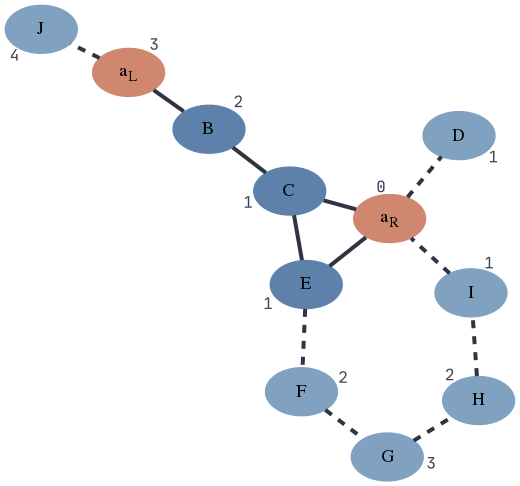
\includegraphics[width=0.7\textwidth]{Chapter1/Figs/pruning.png}
    \caption{An illustration of graph pruning. The graph represents a \dbg{} of a candidate region. Nodes represent \kmer{}s and are arbitrarily labelled, except $a_L$ and $a_R$ (red), which are the start and end anchor \kmer{}s, respectively. When enumerating paths, we aim to find all paths between $a_L$ and $a_R$ with a length no greater than a specified maximum. Numbers next to nodes indicate the length of the shortest path from that node to the end \kmer{} $a_R$. In this example, we set a maximum path length of 4. As such, light blue nodes and dashed edges indicate sections of the graph that would be pruned (not explored).}
    \label{fig:pruning}
\end{figure}

\hspace{0.75cm}

\noindent
In the end, for each candidate region ($r$), we are left with a collection of paths ($V_r$) between two \kmer{}s ($a_L$ and $a_R$). We create the final candidate paths by replacing the sequence between $a_L$ and $a_R$ in the maximum likelihood path ($mlp_n$) with each path ($p_r$) in $V_r$. These are written to file - with one file per candidate region. Padding the candidate paths in this way ensures they are inserted into the \prg{} in the correct location (see \autoref{sec:denovo-insert}). 


\subsection{Updating a \panrg{} with candidate paths}
\label{sec:denovo-insert}

As new paths may alter the structure of a \prg{}, we cannot insert them directly and must rebuild each \prg{} for which a candidate path is discovered.

The first step of rebuilding each locus \prg{} is to add the new candidate paths to the original multiple sequence alignment (MSA). We ensure the novel paths align with the correct section of the locus because we padded each candidate with the maximum likelihood path. Next, we combine all candidate paths for a locus into a single, unaligned FASTA file and add them to the existing locus MSA with the \vrb{--add} protocol in MAFFT \cite{katoh2012}. 

Finally, we run \makeprg{} on the subsequent alignments, and the resulting updated \prg{}s are combined into a single \panrg{} and indexed with \pandora{}. 

This updated \panrg{} can then be used as input to \pandora{}, and subsequent genotyping will include the novel variants.

% ==================================================================
\section{Initial assessment via simulations}
\label{sec:denovo-sims}
Having described an extension of the \pandora{} program that allows for \denovo{} variant discovery, we now perform an initial evaluation and explore the impact of various parameters using a simulated dataset.

\subsection{Methods}
\label{sec:denovo-sims-methods}

The first step in evaluating the effect of adding \denovo{} variant calling to \pandora{} is with a simulated dataset. We aim to show that the addition of \denovo{} discovery allows \pandora{} to improve its capacity for variant detection (recall) with minimal impact on the quality of the calls (precision). 

To construct our simulated dataset, we randomly select 100 gene MSAs from a pool of 29,702 obtained for \ecoli{} from the panX database \cite{panx}. Next, a \prg{} is constructed for each MSA with \makeprg{} (\autoref{sec:make_prg}). We used a range of \makeprg{} maximum nesting levels - 1, 3, 5, and 10 - to investigate whether \prg{} nesting has an impact on our ability to discover novel variants. The \prg{}s are combined into a single \panrg{} for each nesting level. A random path through each \prg{} is selected using \pandora{}, and these sequences are concatenated together to form a single "genome" sequence. 

We subsequently add single nucleotide polymorphisms (SNPs) to the simulated genome at different per-gene rates using \vrb{snp-mutator} \cite{snpmutator}. For this work, we introduce 100, 400, and 1,000 SNPs to the simulated genome, which equate to approximately 1, 4, and 10 SNPs per gene, respectively. \vrb{snp-mutator} produces a VCF of the SNPs that were introduced, along with the mutated genome sequence.

Next, we simulated 30,000 \ont{} reads from the mutated genomes using \vrb{nanosim-h} \cite{yang2017,brinda2018}. As the most recent model offered by \vrb{nanosim-h} was from the old R9 \ont{} flow cell, we trained and used a model from a freely-available \ecoli{} R9.4 dataset (\url{http://lab.loman.net/2017/03/09/ultrareads-for-nanopore/}). Each read set was randomly subsampled to a read depth (coverage) of 15, 30, 60, and 100 with \vrb{rasusa} \cite{rasusa2019} so we can investigate the impact of coverage on our ability to discover novel variants.

\pandora{}'s \vrb{discover} routine is then run, using the original panX-derived \panrg{} and the reads simulated from the mutated genome. Using this approach, we know that the reads originate from a sequence in our \panrg{}, but with some SNP differences and \ont{} errors. It is possible that some of the random SNPs introduced by \vrb{snp-mutator} already exist in the \panrg{}, but this is likely a minimal number. We use three different \kmer{} sizes for the \denovo{} discovery: 11, 13, and 15. 

After running the \vrb{discover} routine, we are left with a collection of candidate paths produced by the \denovo{} component. We then add these candidate paths back into the \panrg{} as per \autoref{sec:denovo-insert}. The updated \panrg{} is then used as input - along with the simulated reads - to \pandora{} \vrb{map} to produce a genotyped VCF that hopefully contains all of the simulated SNPs.

In parallel to this, we also run \pandora{} \vrb{map} on the original \panrg{} and simulated reads - i.e., without variant discovery. The genotyped VCF produced by this run shows how \pandora{} performed before the addition of \denovo{} variant discovery in this chapter. Theoretically, we only expect this VCF to contain simulated SNPs that were already in the \panrg{}.

At the end of this workflow, we have a genotyped VCF with and without \denovo{} variant discovery for each combination of maximum nesting, \denovo{} \kmer{} size, SNP rate, and read depth (coverage).

\subsection{Evaluation}
\label{sec:denovo-sims-eval}

Comparing the truth VCF to the one produced by \pandora{} requires care. The variants in the truth VCF are with respect to a linear reference genome; as we only simulated SNPs, these are single-position records. However, the \pandora{} variants are with respect to a graph and, depending on the density of variation in the graph, may not appear as single-position records (see \autoref{fig:min-match-len-example} for an illustration of this). 

We avoid the error-prone conversion of linear coordinates into graph coordinates, or vice versa, by using a coordinate-free evaluation. This approach maps variant \emph{probes} to each other and compares the probe sequences.  

We define a probe-set $P$ as a collection of probes, $p$, where $p$ represents an entry, $e$, in a VCF file, $V$. For each $e \in V$, $p$ is constructed by the concatenation of $l_w$, $e_c$, and $r_w$ (in that order), where $e_c$ is the called allele of $e$, and $l_w$ and $r_w$ are the sequences, of maximum length $w$, in the VCF reference to the left and right, respectively, of $e_c$. For \pandora{}, the VCF reference is the maximum likelihood sequence, and for the truth VCF it is the simulated genome (without the simulated SNPs).

A truth probe-set, $P_t$, was constructed from the VCF of variants added to the simulated genome and a query probe-set, $P_q$, from the variants called by \pandora{}. We then mapped all probes from $P_t$ to $P_q$ using \vrb{bwa mem} \cite{li2013}. We classify each probe in $P_t$ as a true positive (TP) if the $e_c$ part of the probe exactly matches the sequence it aligns to in $P_q$, or a false negative (FN) otherwise. Any probe in $P_q$ that does not have a TP truth probe mapped to it is classified as a false positive (FP). We perform this assessment for the "no \denovo{}" and "with \denovo{}" VCF files from \pandora{}. 

Precision is defined as the number of TPs divided by the number of TPs and FPs $precision=\frac{TP}{TP+FP}$; it represents the fraction of variant calls made that are correct. Likewise, recall is calculated as $recall=\frac{TP}{TP+FN}$ and describes the proportion of expected variants correctly discovered.

\subsection{Results}
\label{sec:denovo-sims-results}

We first look at \autoref{fig:denovo-sims}, which shows how precision and recall of the \pandora{} \denovo{} variants changes depending on the combination of parameters chosen. Those parameters were the read depth (coverage) of the simulated reads (\autoref{fig:denovo-sims-covg}), the number of SNPs introduced into the simulated genome (\autoref{fig:denovo-sims-num-snps}), the \kmer{} size used for variant discovery (\autoref{fig:denovo-sims-kmer-size}), and the maximum nesting level allowed in the \prg{}s (\autoref{fig:denovo-sims-nesting}). In total, there are 144 different combinations of parameters, and thus data points.

The parameter that appears to have the most visible impact on the precision and recall is the coverage (\autoref{fig:denovo-sims-covg}). It is somewhat unsurprising that as coverage increases, so do both precision and recall. However, there does not seem to be any noticeable difference for coverage $\ge 60$.

In the best case, the highest recall and precision values are 0.91 and 1.0, respectively. The data point is the same in both instances, with a coverage of 60, \kmer{} size of 13, number of SNPs 100, and a maximum nesting level of 10. Upon further investigation of the nine missed variants (FNs) for this data point, six were within $2k-1$ positions of the start or end of the locus, one was a null call (indicating genotyping uncertainty), one was falsely called as a homopolymer deletion, and the remaining missed call never had \denovo{} discovery triggered for that region of the locus. Therefore, only 3/9 FNs for this example (the last three) were discoverable with our \denovo{} method.

The last point requires some elaboration, as it may not be clear why only three FNs in the best-performing data point were expected to be detected by \denovo{}. As a reminder, the role of the \denovo{} component is to collect candidate alleles that are potentially in the sample but missing from the graph; if that set includes the truth, it has succeeded. Whether or not that true allele is genotyped as being present and recorded in the VCF is the job of the sequence inference and genotyping components of \pandora{}. In the case of the null genotype call, the correct variant was discovered, and it had higher coverage than the reference allele (26 vs 11); therefore, it is a failure of the genotyping. The homopolymer deletion is a failure of the genotyping; while \denovo{} (incorrectly) discovered the candidate indel, it also discovered the correct allele, but the genotyping chose the homopolymer deletion. Furthermore, the variant which \denovo{} discovery was never initiated for most likely has enough coverage on the reference allele that a candidate region was not detected - by default, we only flag a candidate region if coverage drops below 3.

In the case of the six missed calls near the ends of loci, these are not detectable by our current \denovo{} method as they occur within $2k-1$ positions of the boundary of a locus. The reason this makes them undetectable is related to our need for start and end anchor \kmer{}s in order to find candidate paths (\autoref{sec:path-enum}). The start and end \kmer{}s are a collection of $k$ \kmer{}s, meaning $2k-1$ positions are required surrounding a candidate region in order to be able to initiate \denovo{} discovery. We will return to this limitation later (\autoref{sec:fw-path-enum}).

\begin{figure}
     \centering
     \begin{subfigure}[b]{0.475\textwidth}
        \centering
        \caption[position=above]{Simulated coverage (read depth)}
        \label{fig:denovo-sims-covg}
        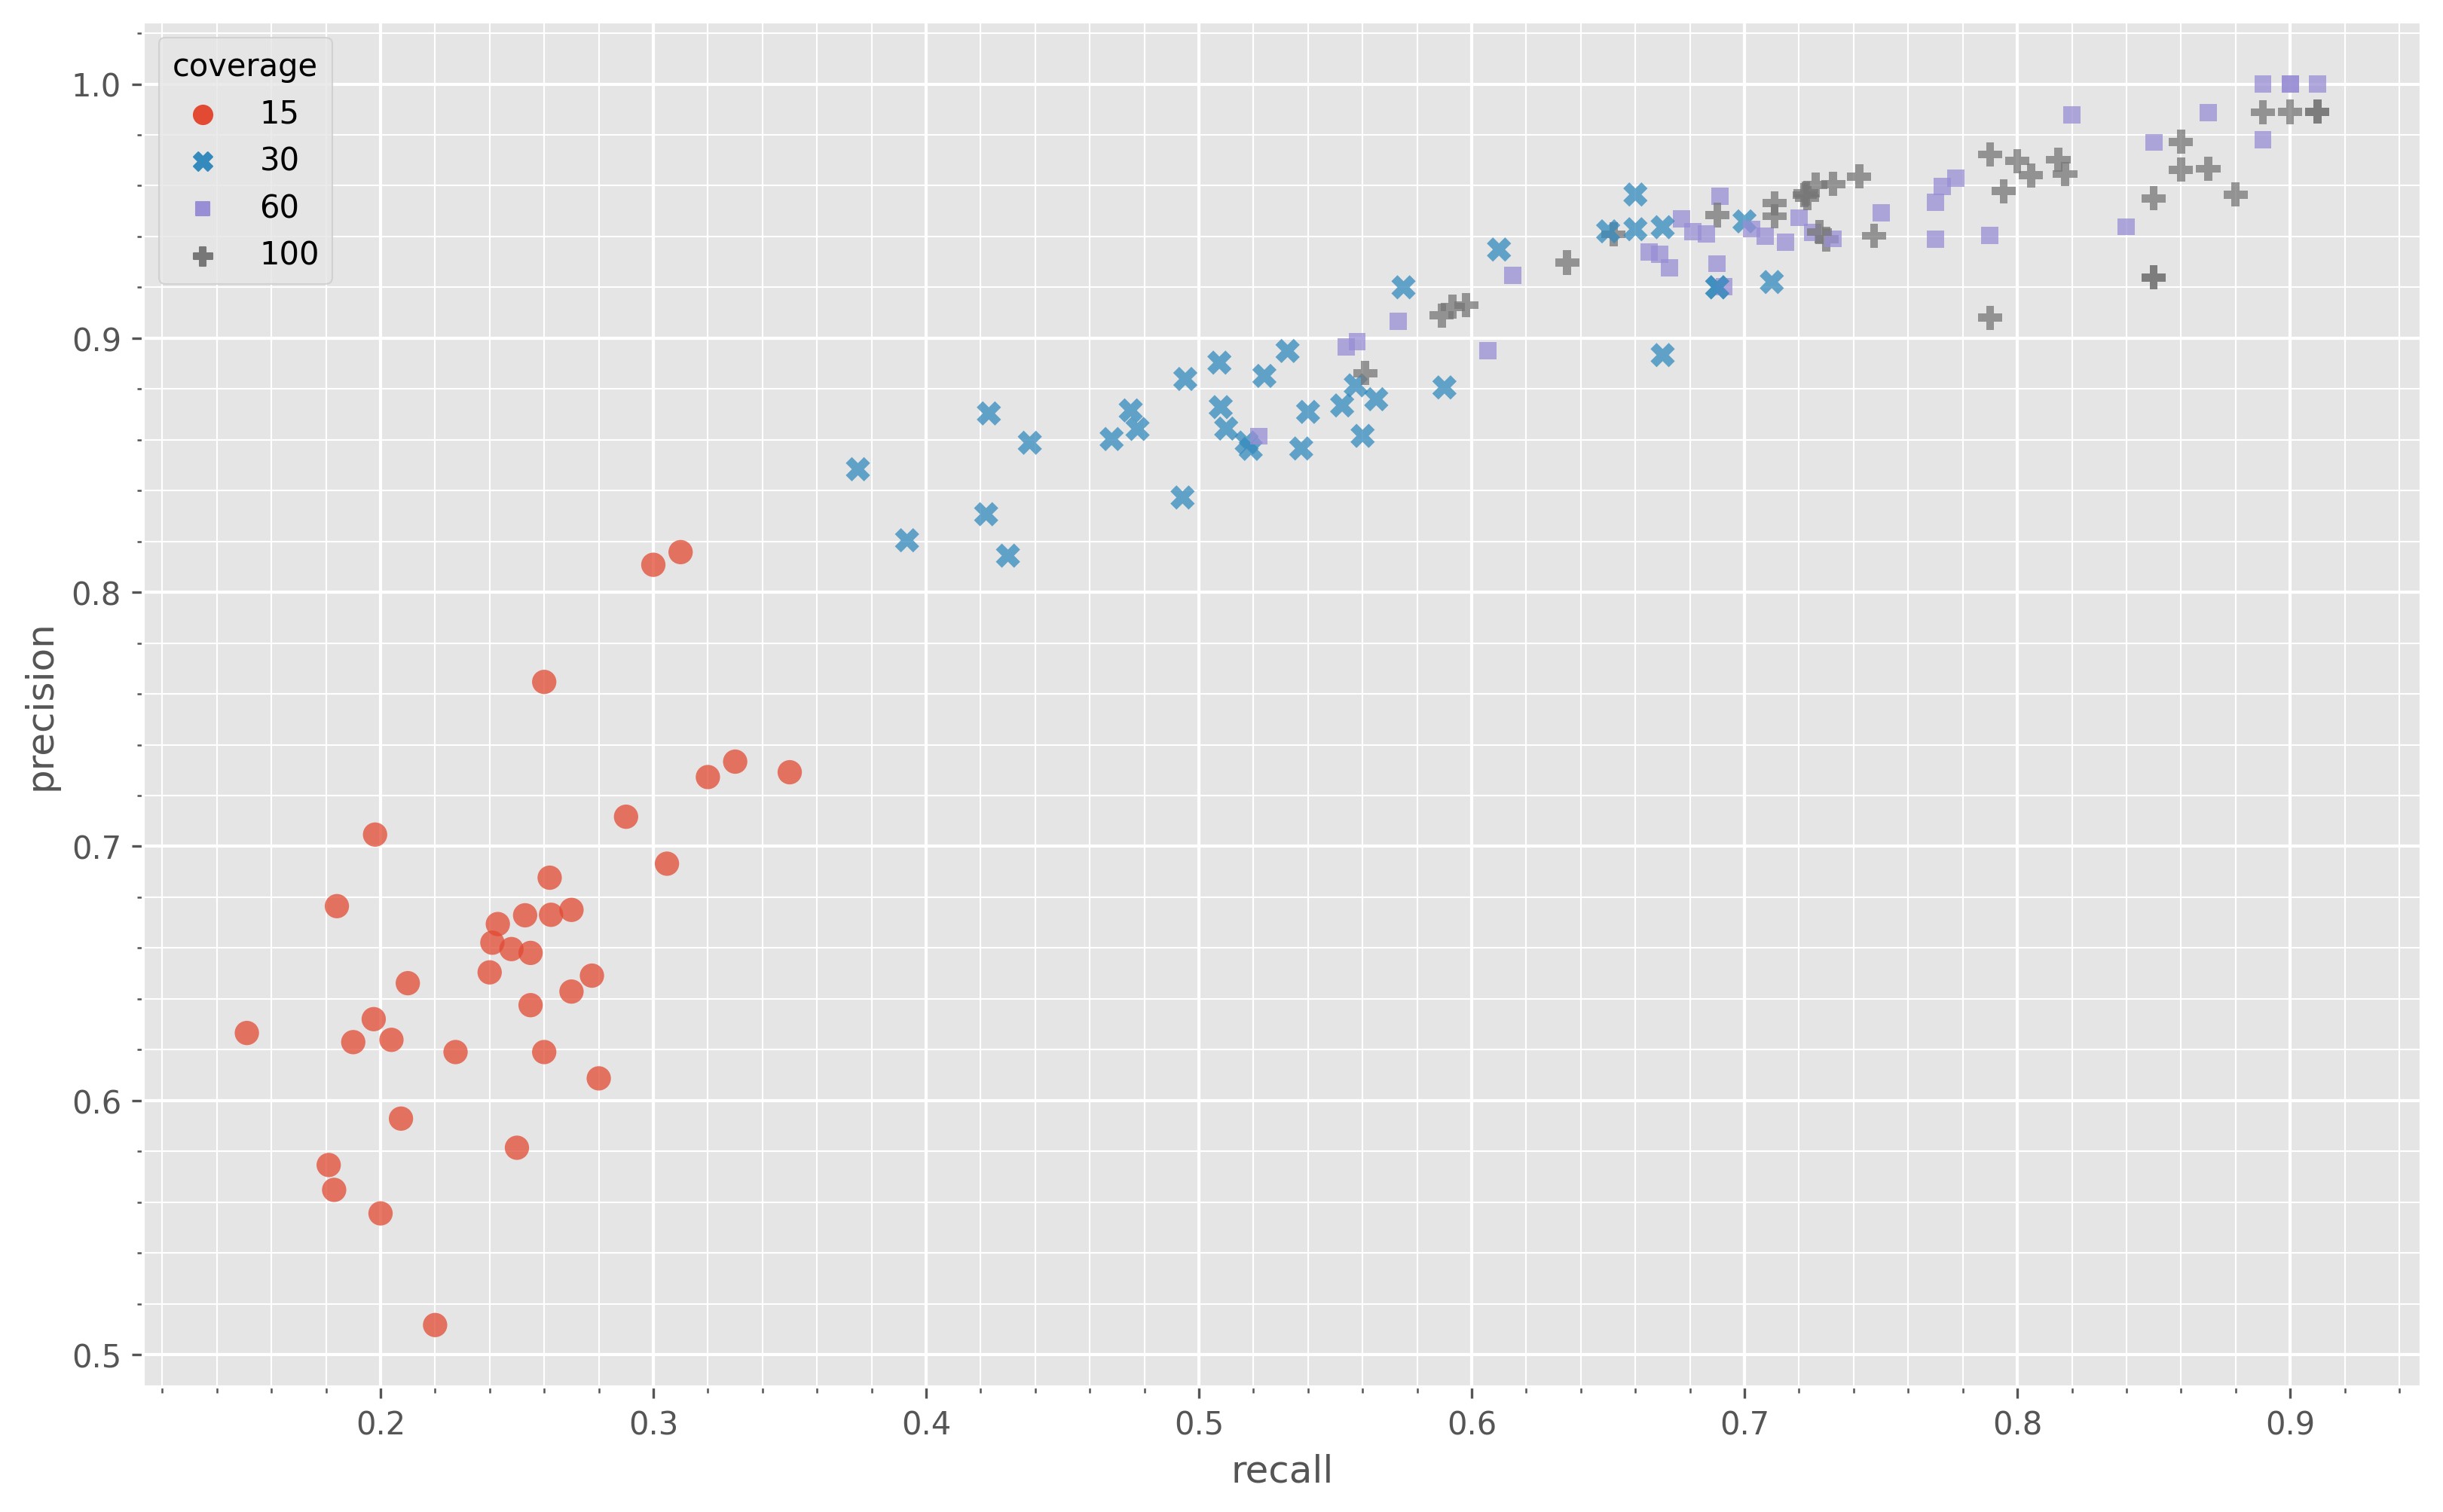
\includegraphics[width=1\linewidth]{Chapter1/Figs/denovo_precrec_covg.png}
     \end{subfigure}
     \begin{subfigure}[b]{0.475\textwidth}
         \centering
          \caption[position=above]{Number of SNPs simulated}
         \label{fig:denovo-sims-num-snps}
        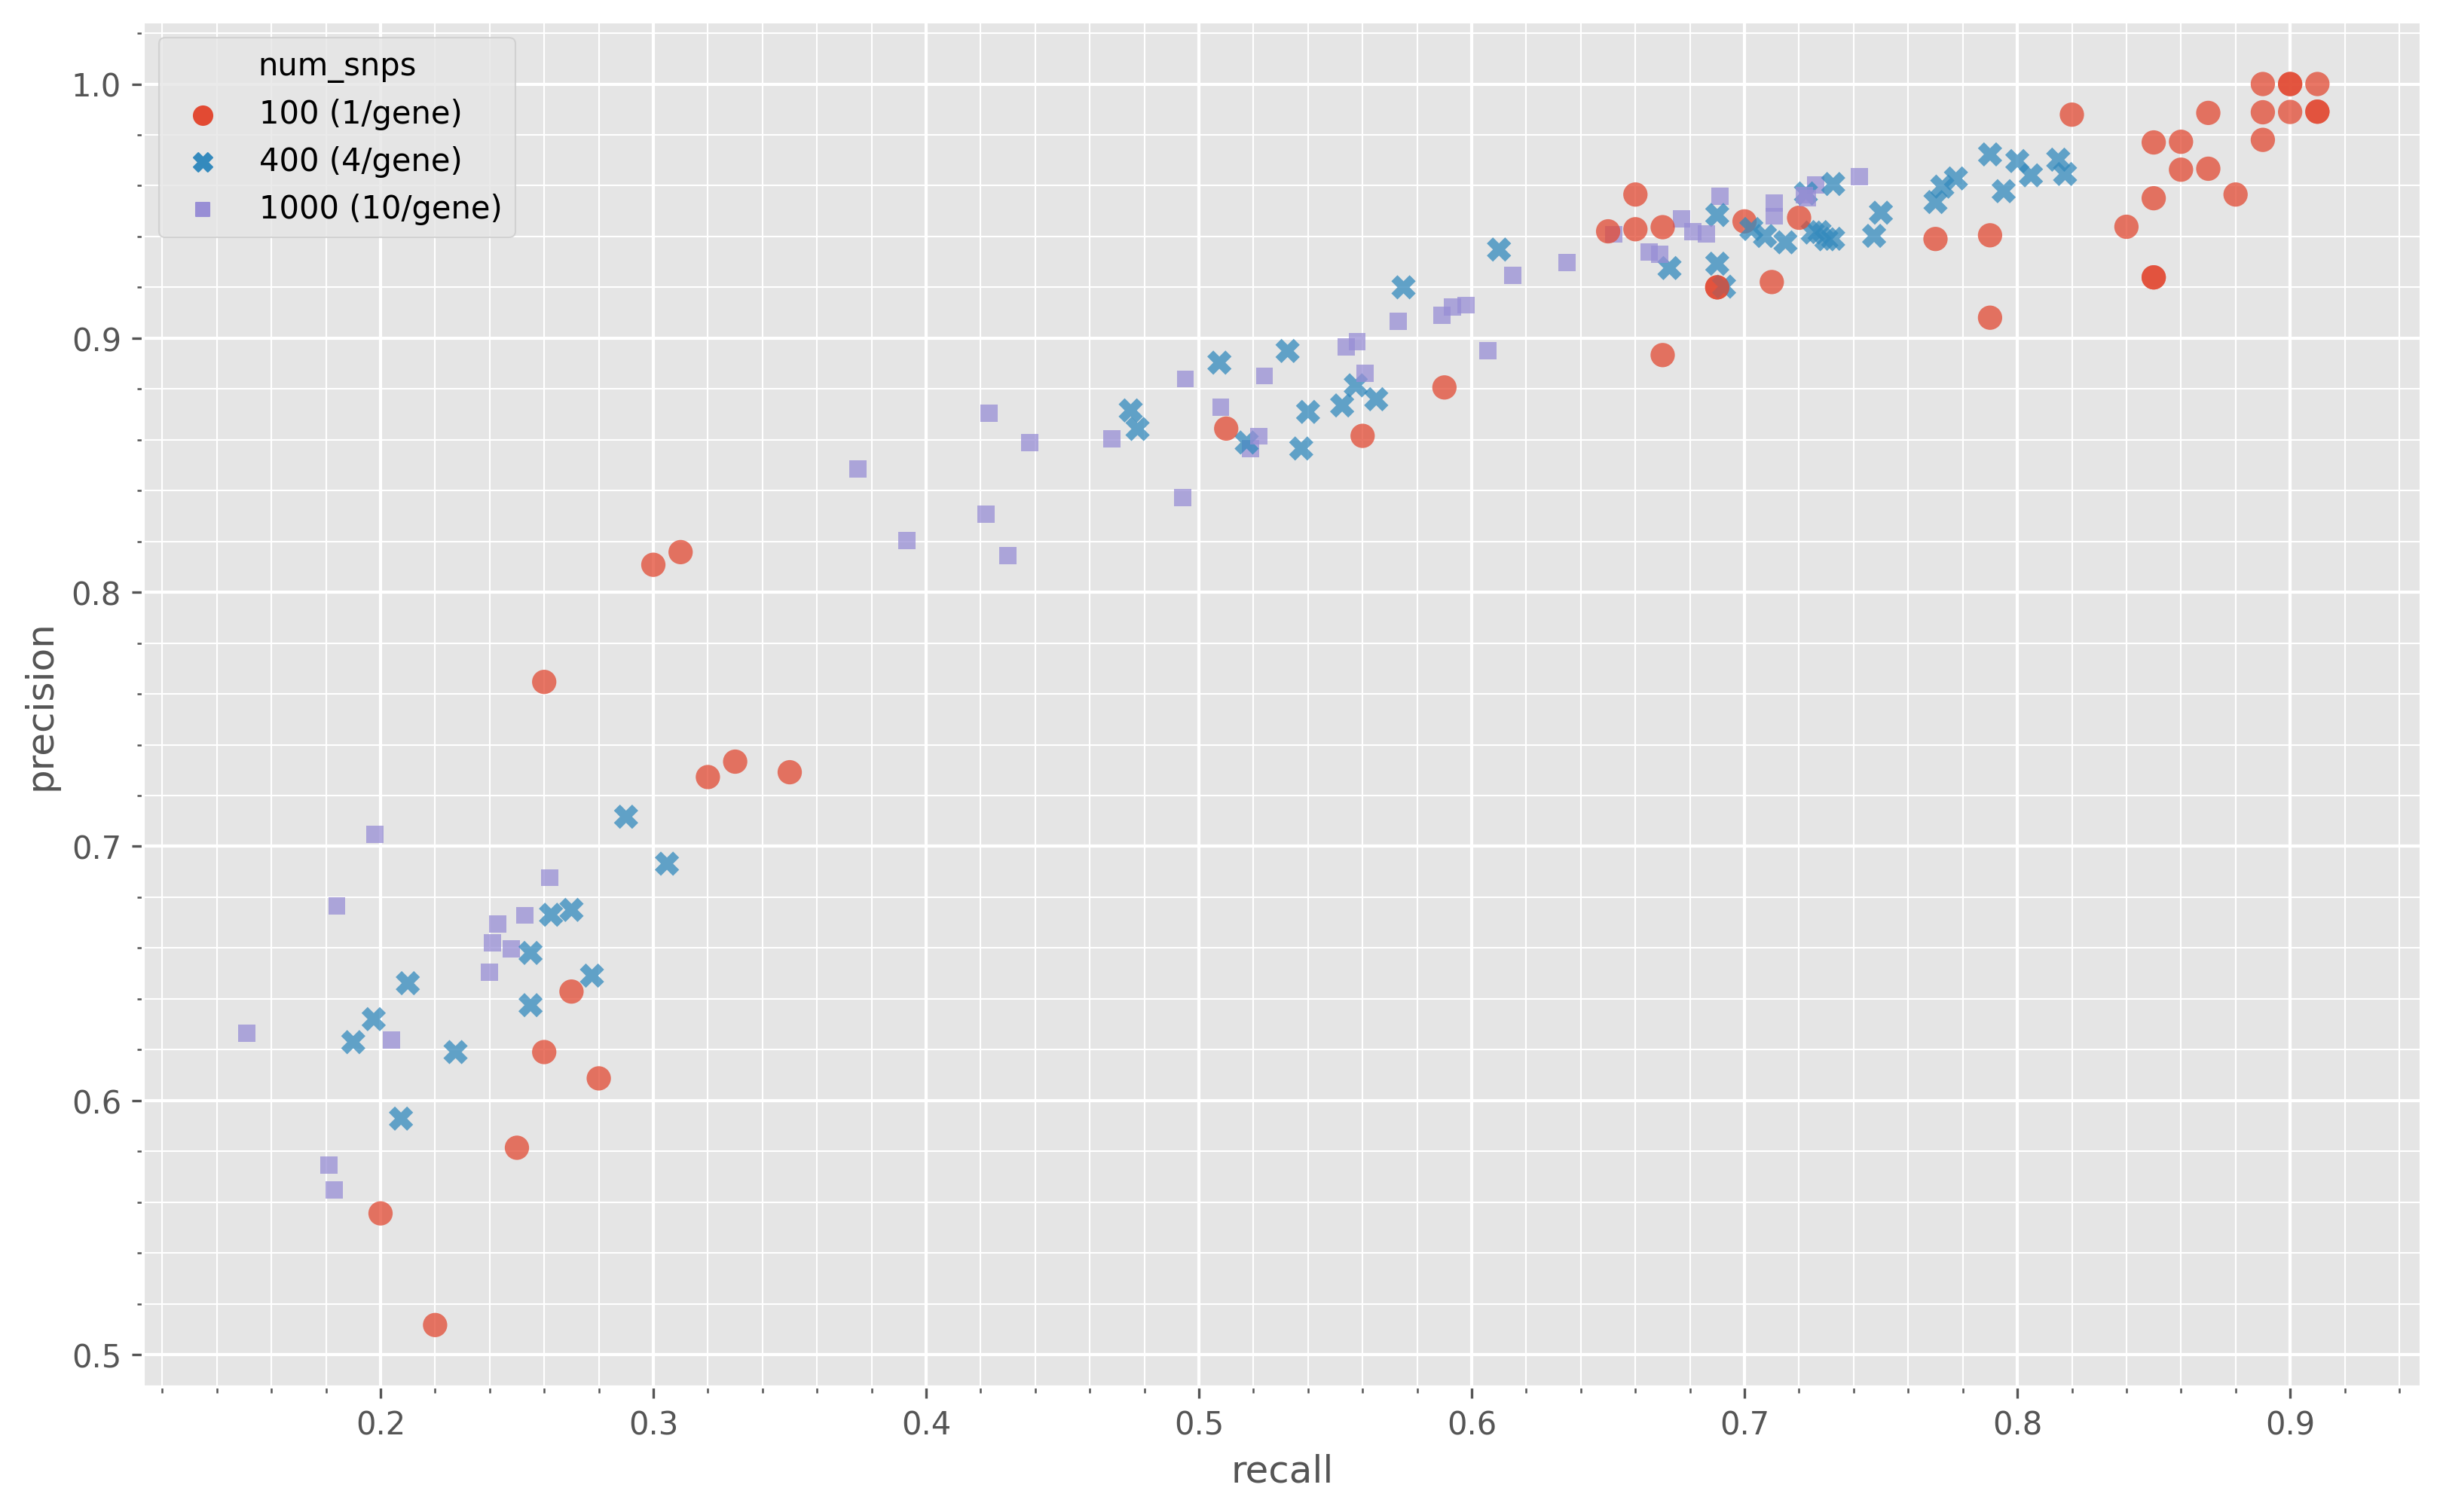
\includegraphics[width=1\linewidth]{Chapter1/Figs/denovo_precrec_num_snps.png}
     \end{subfigure}
     \begin{subfigure}[b]{0.475\textwidth}
         \centering
        \caption[position=above]{\denovo{} discovery \kmer{} size}
        \label{fig:denovo-sims-kmer-size}
        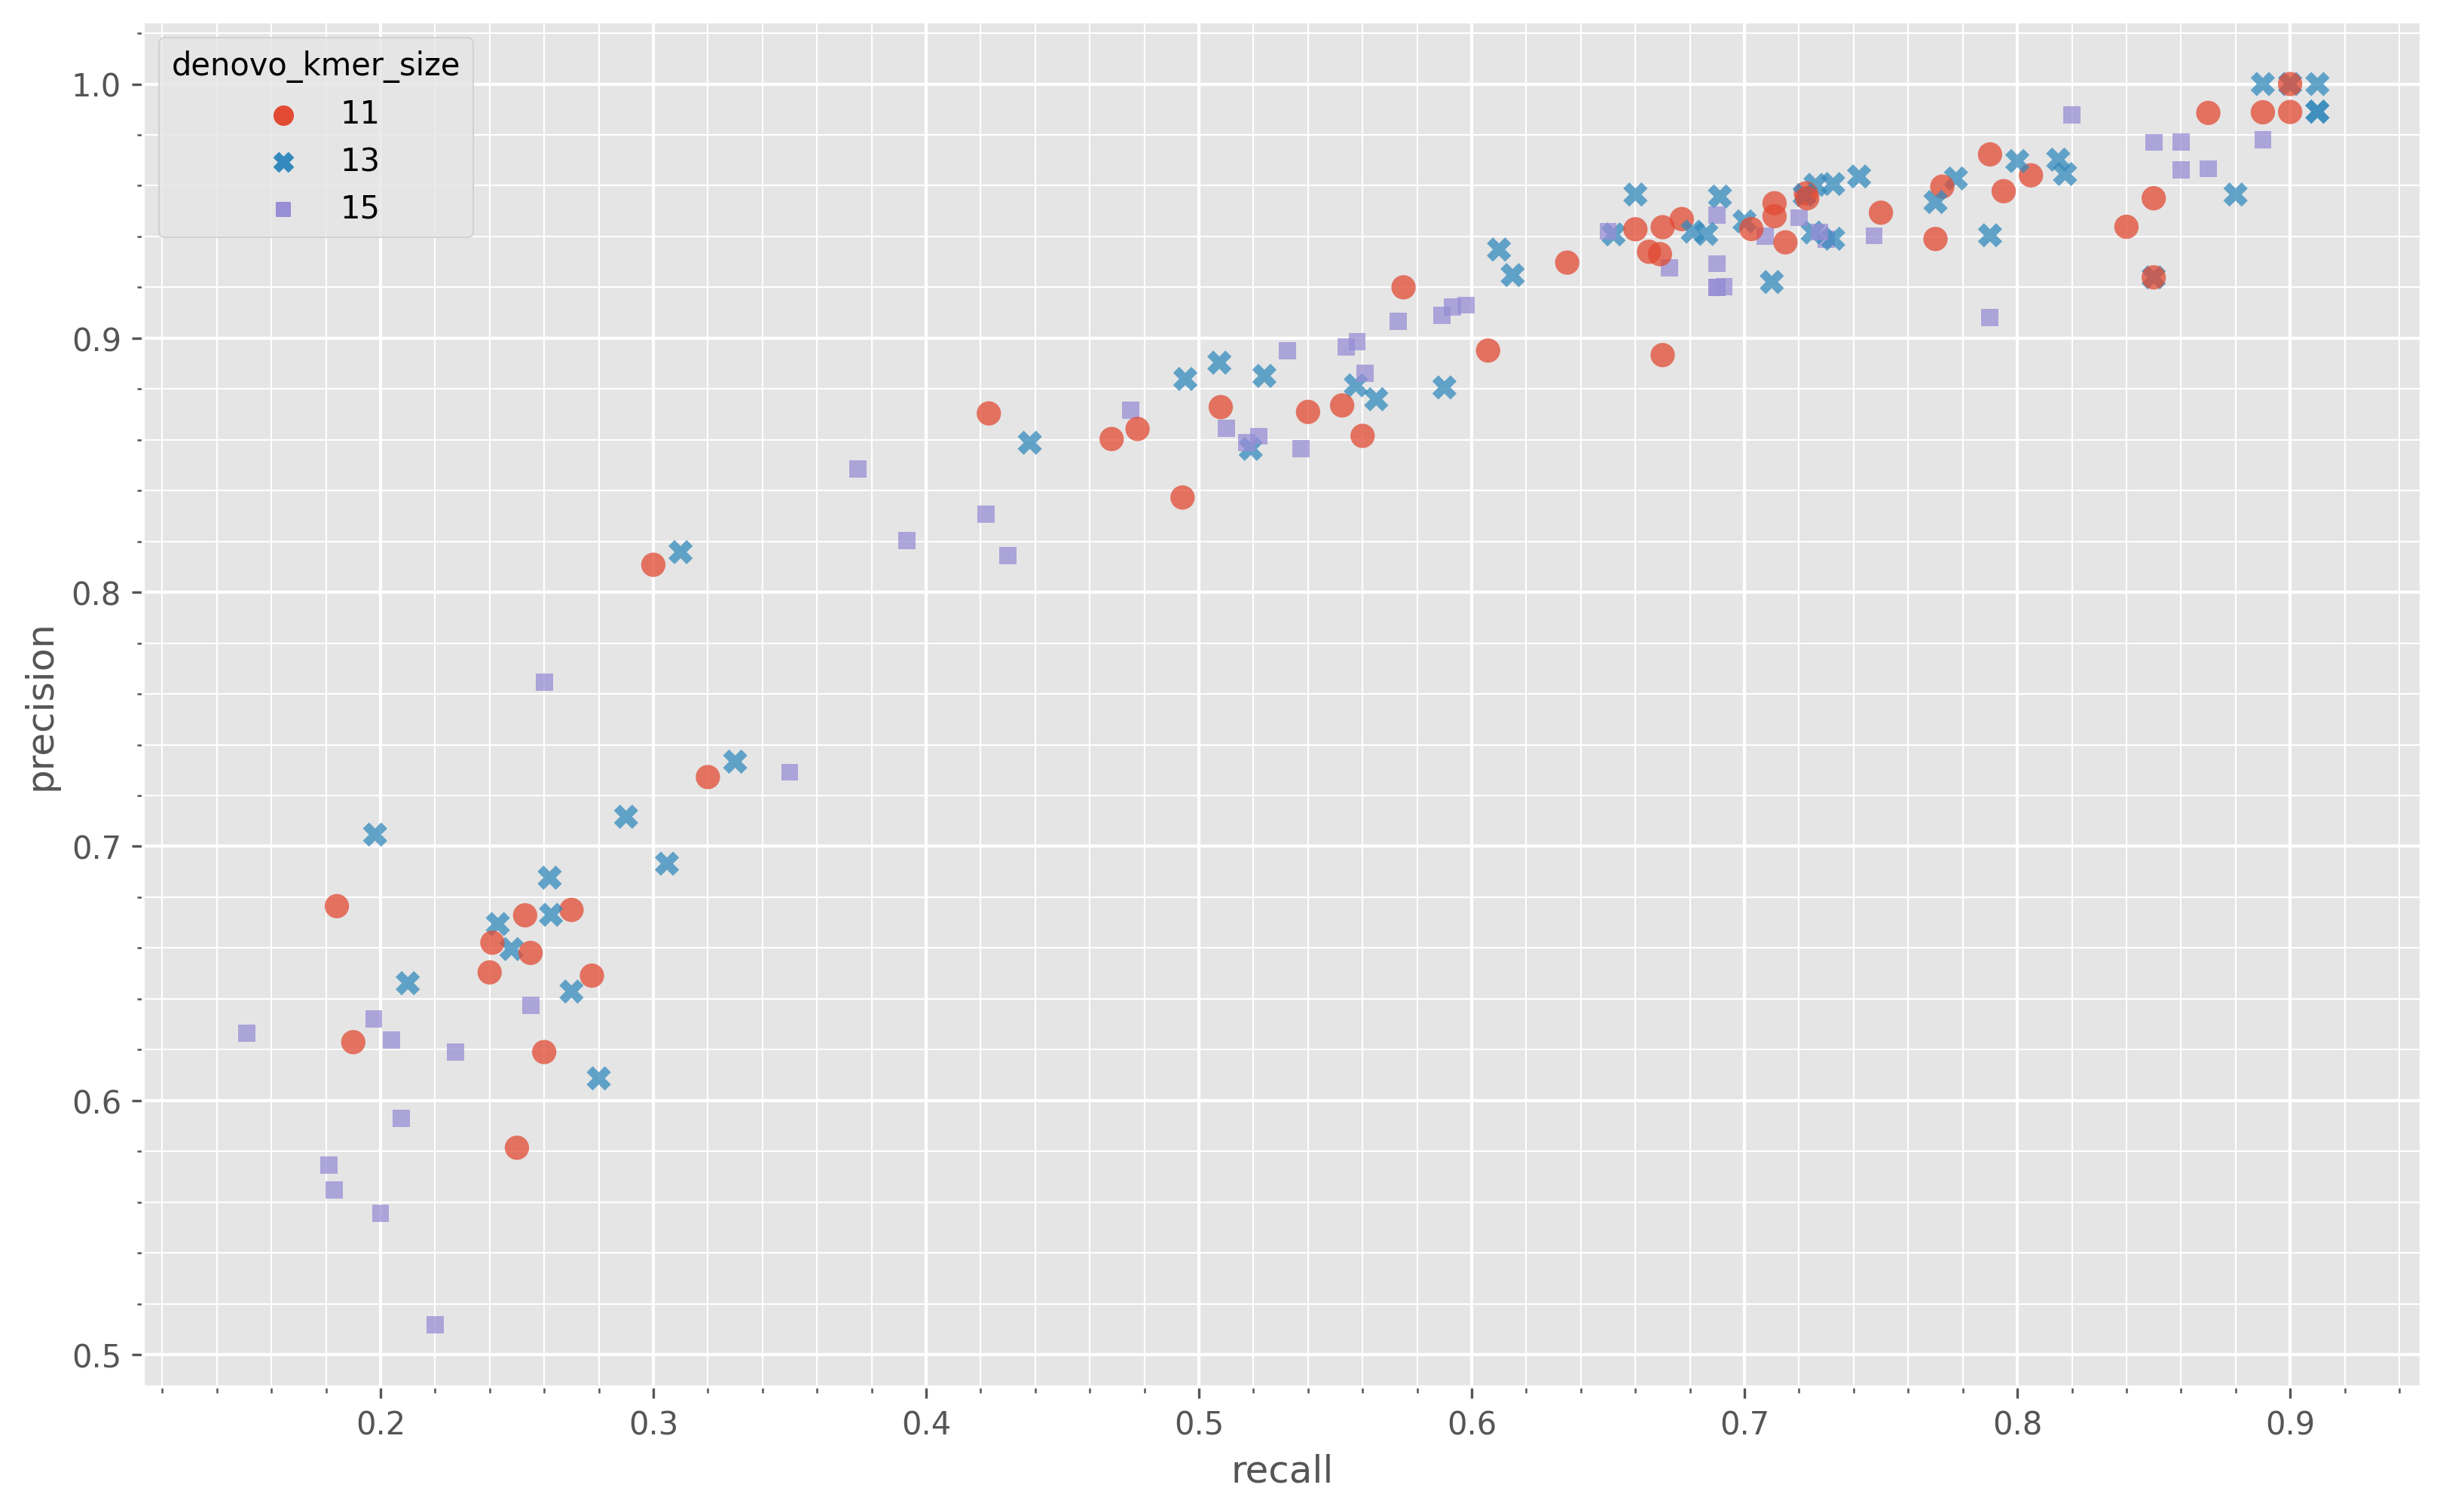
\includegraphics[width=1\linewidth]{Chapter1/Figs/denovo_precrec_kmer.png}
     \end{subfigure}
     \begin{subfigure}[b]{0.475\textwidth}
         \centering
         \caption[position=above]{\prg{} maximum nesting level}
         \label{fig:denovo-sims-nesting}
        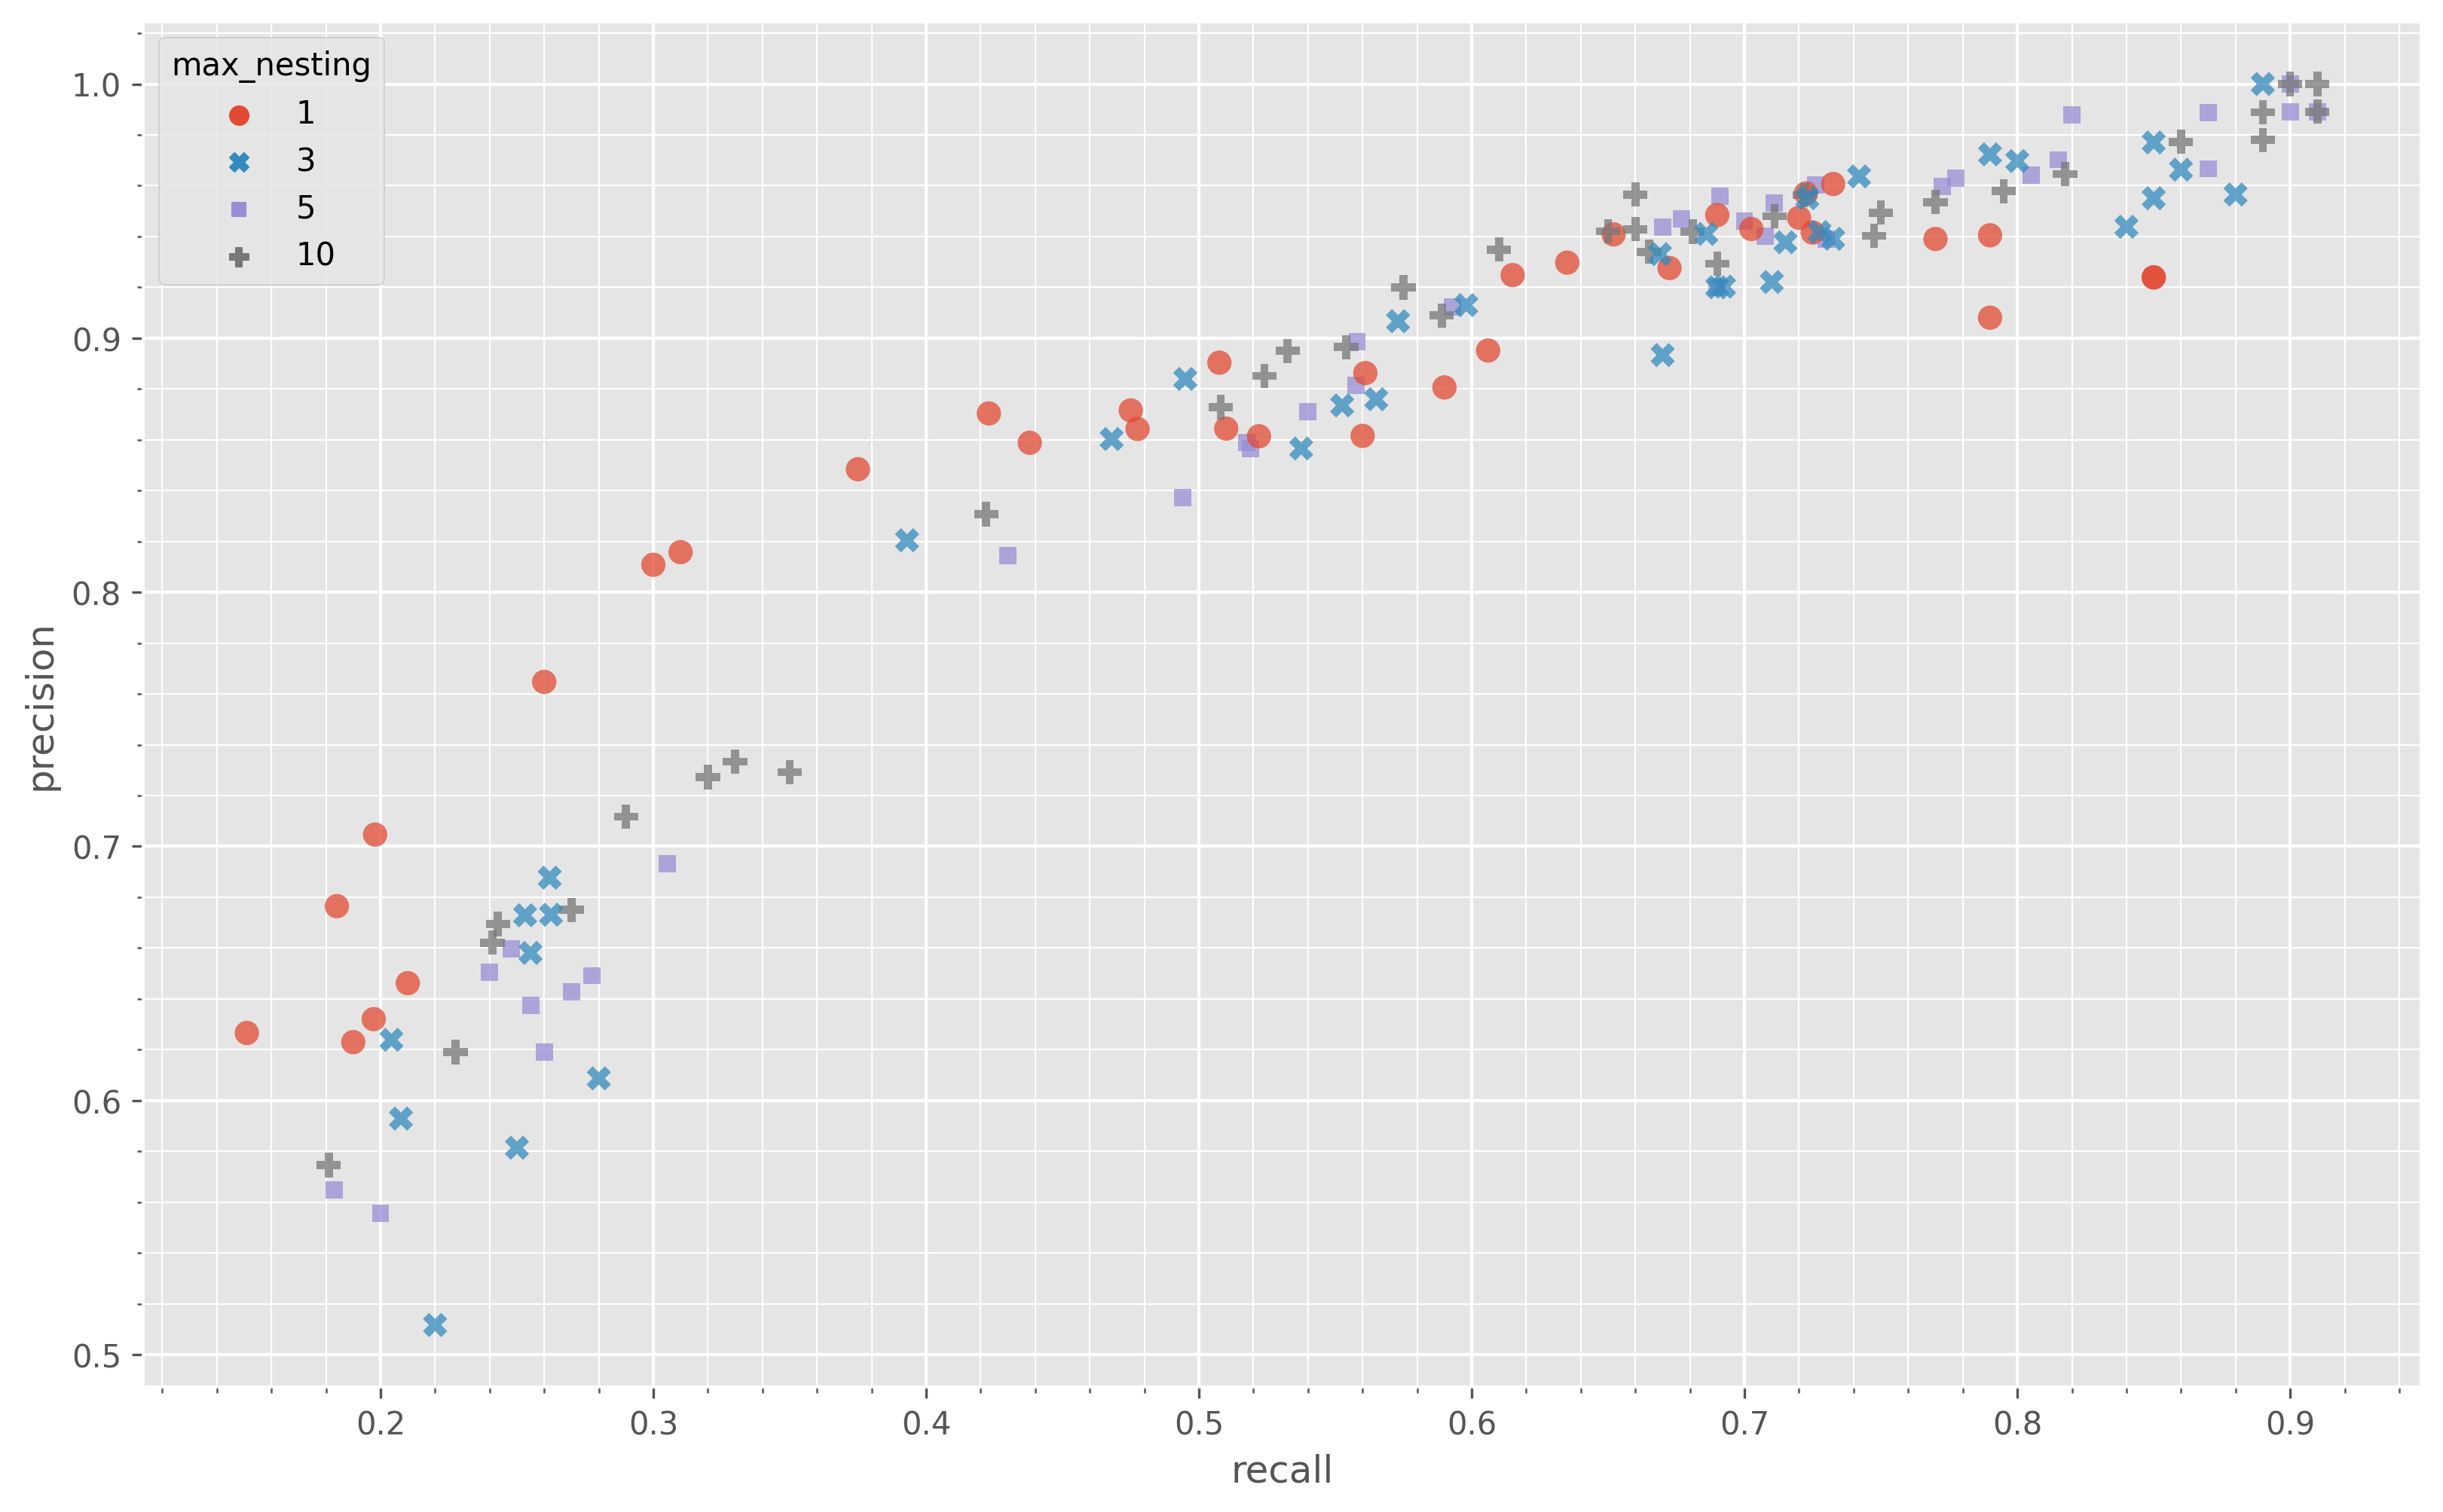
\includegraphics[width=1\linewidth]{Chapter1/Figs/denovo_precrec_nesting.png}
     \end{subfigure}
    \caption{Recall (x-axis) and precision (y-axis) of \denovo{} variants discovered by \pandora{} on a simulated dataset. Subplots style the points by the parameter indicated in the subtitle. Each point indicates a single run of \pandora{} with a unique combination of all parameters.}
        \label{fig:denovo-sims}
\end{figure}

While not an issue for the best-performing example we have just been examining, missing loci were another common source of FNs. If \pandora{} decides a locus is not present after quasi-mapping (\autoref{sec:pandora-intro}), then it is impossible for \denovo{} to discover any variants in it. We note that the vast majority of missing loci have a length of less than 250 base pairs (\autoref{app:denovo-missing-lengths}).

When looking across all 144 combinations of parameters, we found that, on average, 7.8\% of the true variants are near the ends of loci and 2.8\% are in absent loci (see \autoref{fig:denovo-errors}). 

\begin{figure}
    \centering
    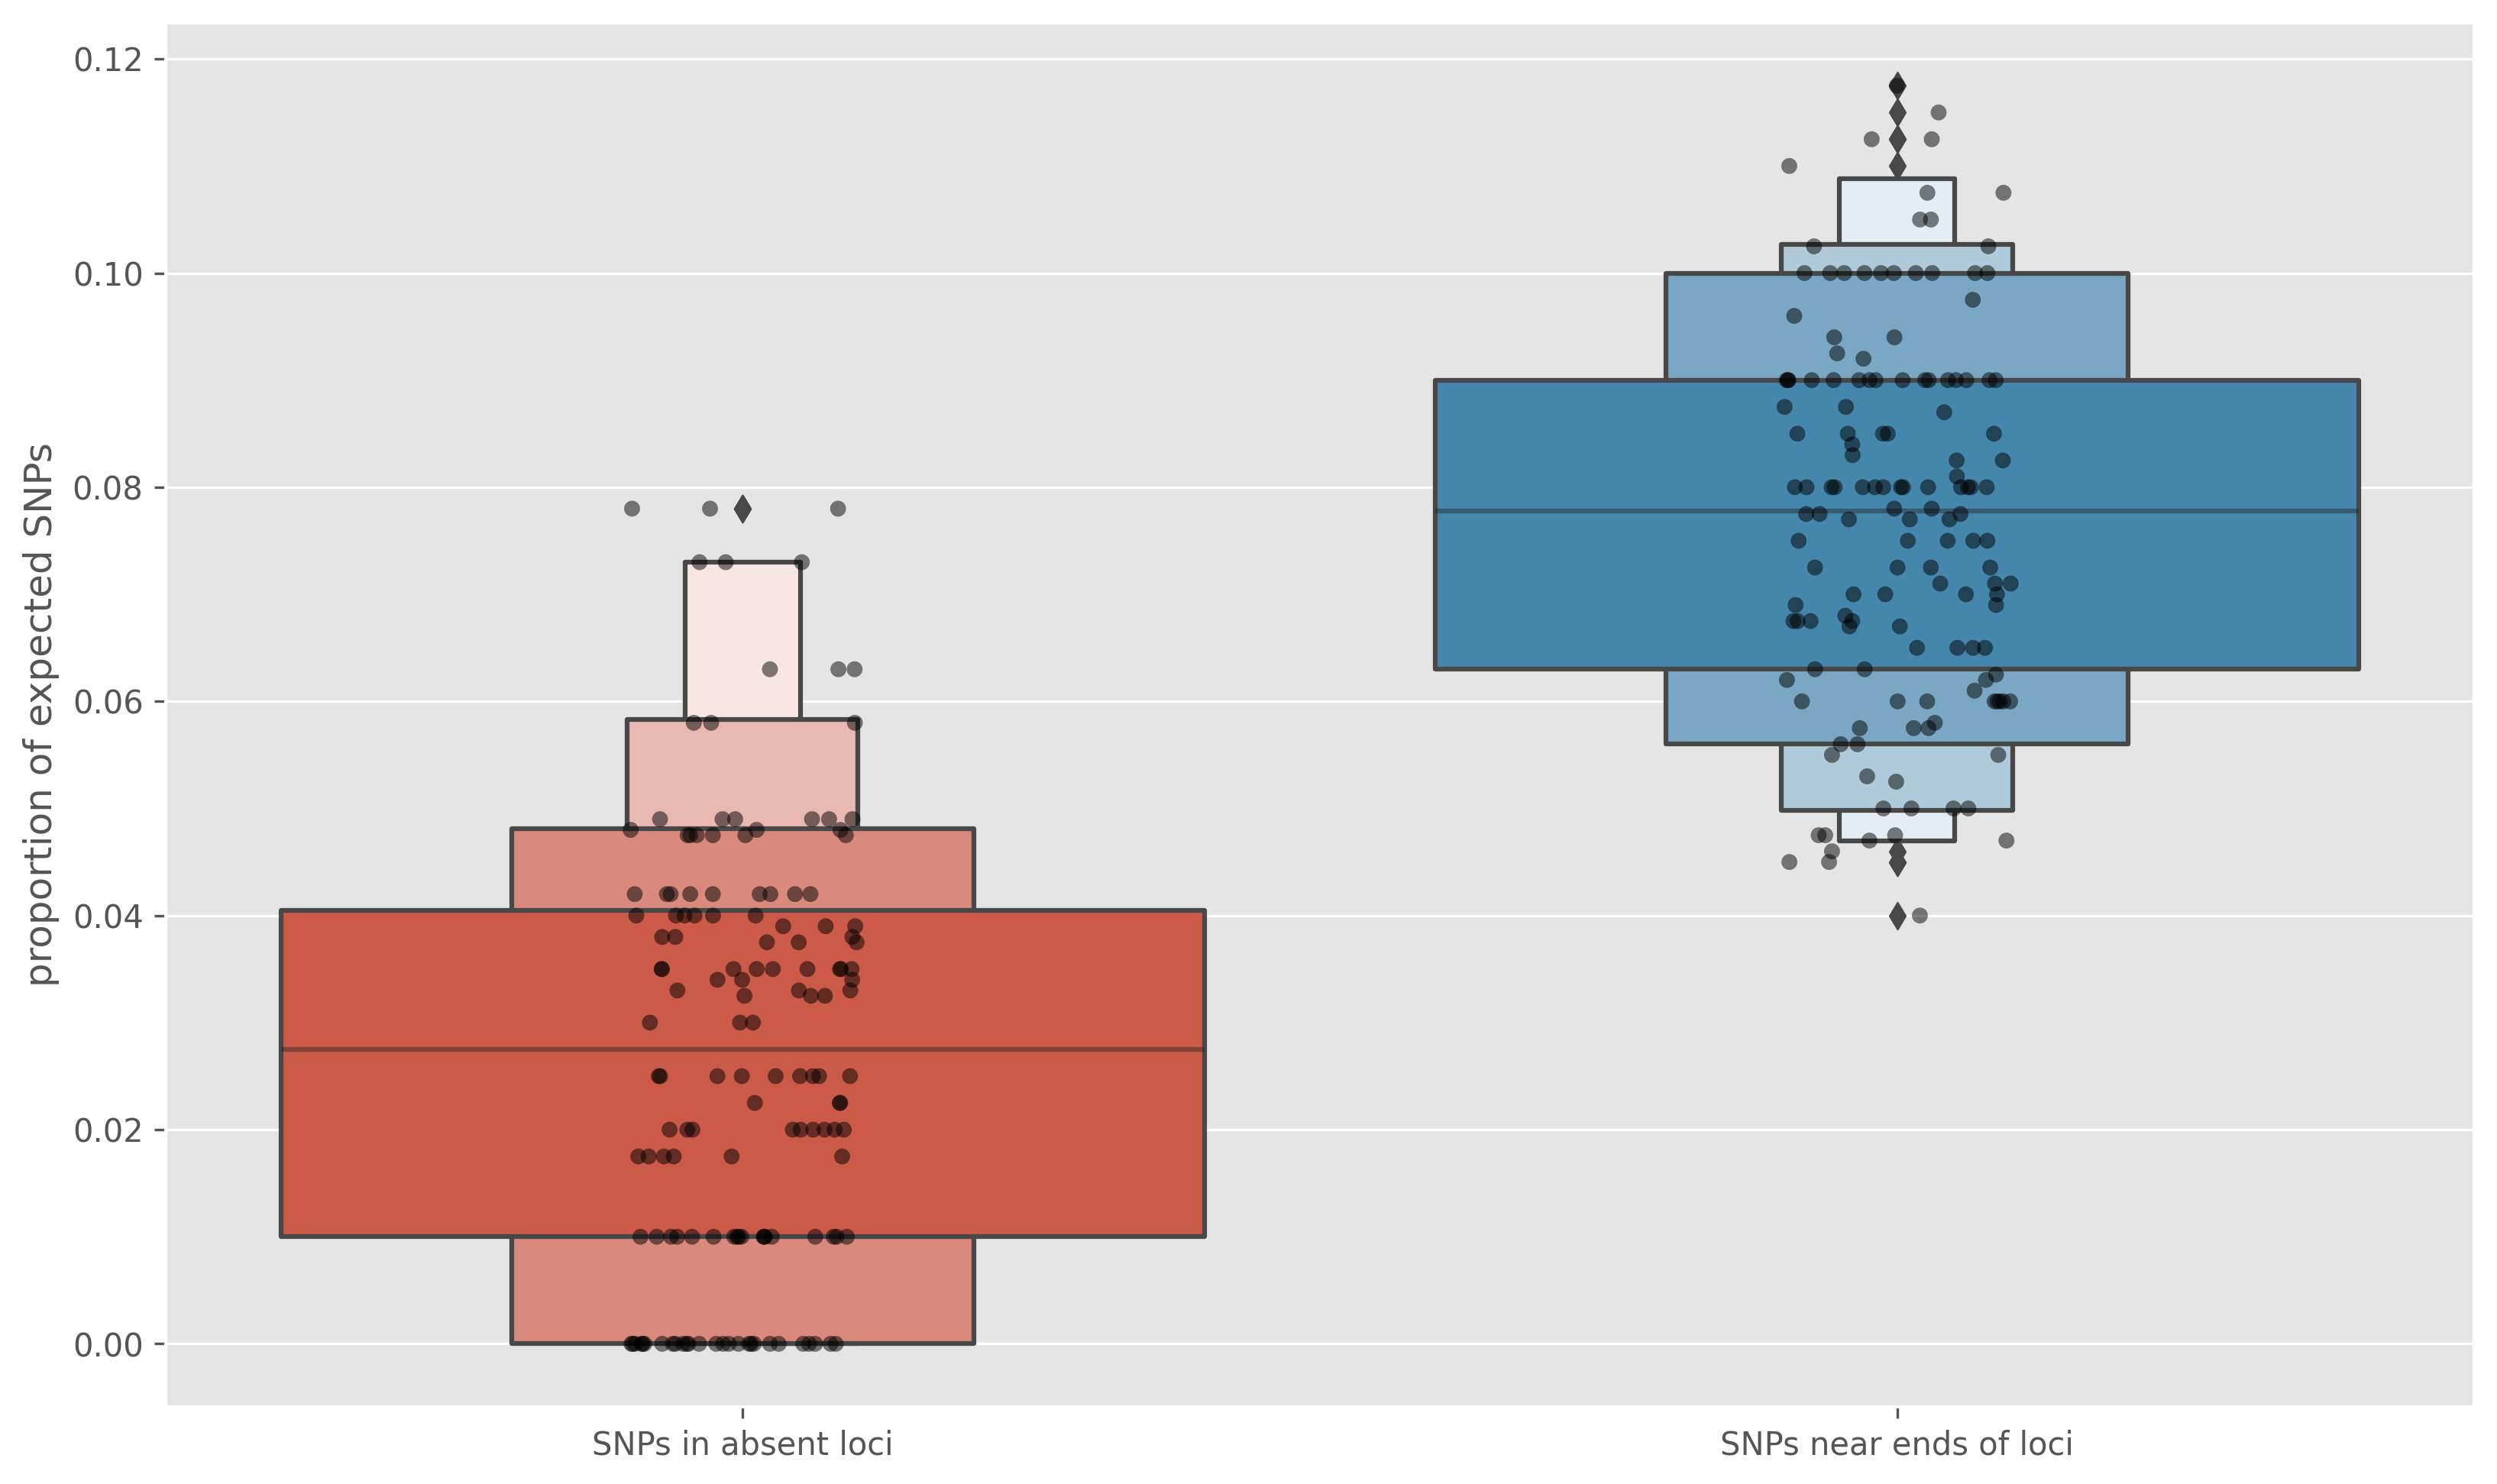
\includegraphics[width=0.9\textwidth]{Chapter1/Figs/denovo_errors.png}
    \caption{The proportion of simulated SNPs that are not detectable by \denovo{} variant discovery. The red box represents SNPs that occur in loci designated as absent by \pandora{}. The blue box depicts the SNPs that occur within $2k-1$ positions of the start or end of a locus. Each point indicates a single run of \pandora{} with a unique combination of parameters.}
    \label{fig:denovo-errors}
\end{figure}

\noindent
The parameters that we can directly control with respect to \denovo{} discovery within \pandora{} are the \prg{} maximum nesting level and the \denovo{} \kmer{} size. \autoref{fig:denovo-sims} shows no clear optimum for either of these options. However, when taking the median precision and recall values across all data points (\autoref{tab:denovo-summary}), a maximum nesting level of 5 and \denovo{} \kmer{} size of 13 seem the best choice.

\begin{table}
\centering
\begin{tabular}{@{}lll@{}}
\toprule
          & Max. nesting & \denovo{} \kmer{} size \\ \midrule
Precision & 0.934 (10)   & 0.937 (13)                                               \\
Recall    & 0.674 (5)    & 0.671 (13)                                               \\ \bottomrule
\end{tabular}
\caption{The median precision and recall for all parameter combinations, grouping by the maximum \prg{} nesting level or the \denovo{} \kmer{} size used for variant discovery in \pandora{}. The values in parentheses indicate the parameter value that leads to the specified precision or recall.}
\label{tab:denovo-summary}
\end{table}

For the final analysis of the simulation data, we look at how the precision and recall change with an increasing genotype confidence threshold. We select the data point with the optimal maximum nesting level (5) and \denovo{} \kmer{} size (13), along with 4 SNPs per gene, as this is within the range expected for an \ecoli{} genome. Next, starting at 0 and increasing by 10 until 700, we filter out any variant with a genotype confidence score below the current threshold. The purpose of this analysis is to illustrate what the cost on recall is for requiring more confident variant calls at different read depths.

\autoref{fig:denovo-sims-roc} shows the same relationship we saw earlier: coverage has a significant impact on precision and recall. Most importantly, though, it shows that the inclusion of \denovo{} discovery is vital for finding novel variants. Precision and recall for \pandora{} \emph{without} variant discovery are not shown in \autoref{fig:denovo-sims-roc}, as the best recall achievable for this set of parameters was only 1.0\% (indicating that 4 SNPs were incidentally in the \panrg{}). This is compared to a maximum of 81.5\% when using \denovo{} discovery. Focusing on the 100x coverage data point with \denovo{} discovery, the best recall (81.5\%) leads to a precision of 97.0\%, but the cost of increasing precision to 99\% is decreasing recall to 25\%. 

\begin{figure}
    \centering
    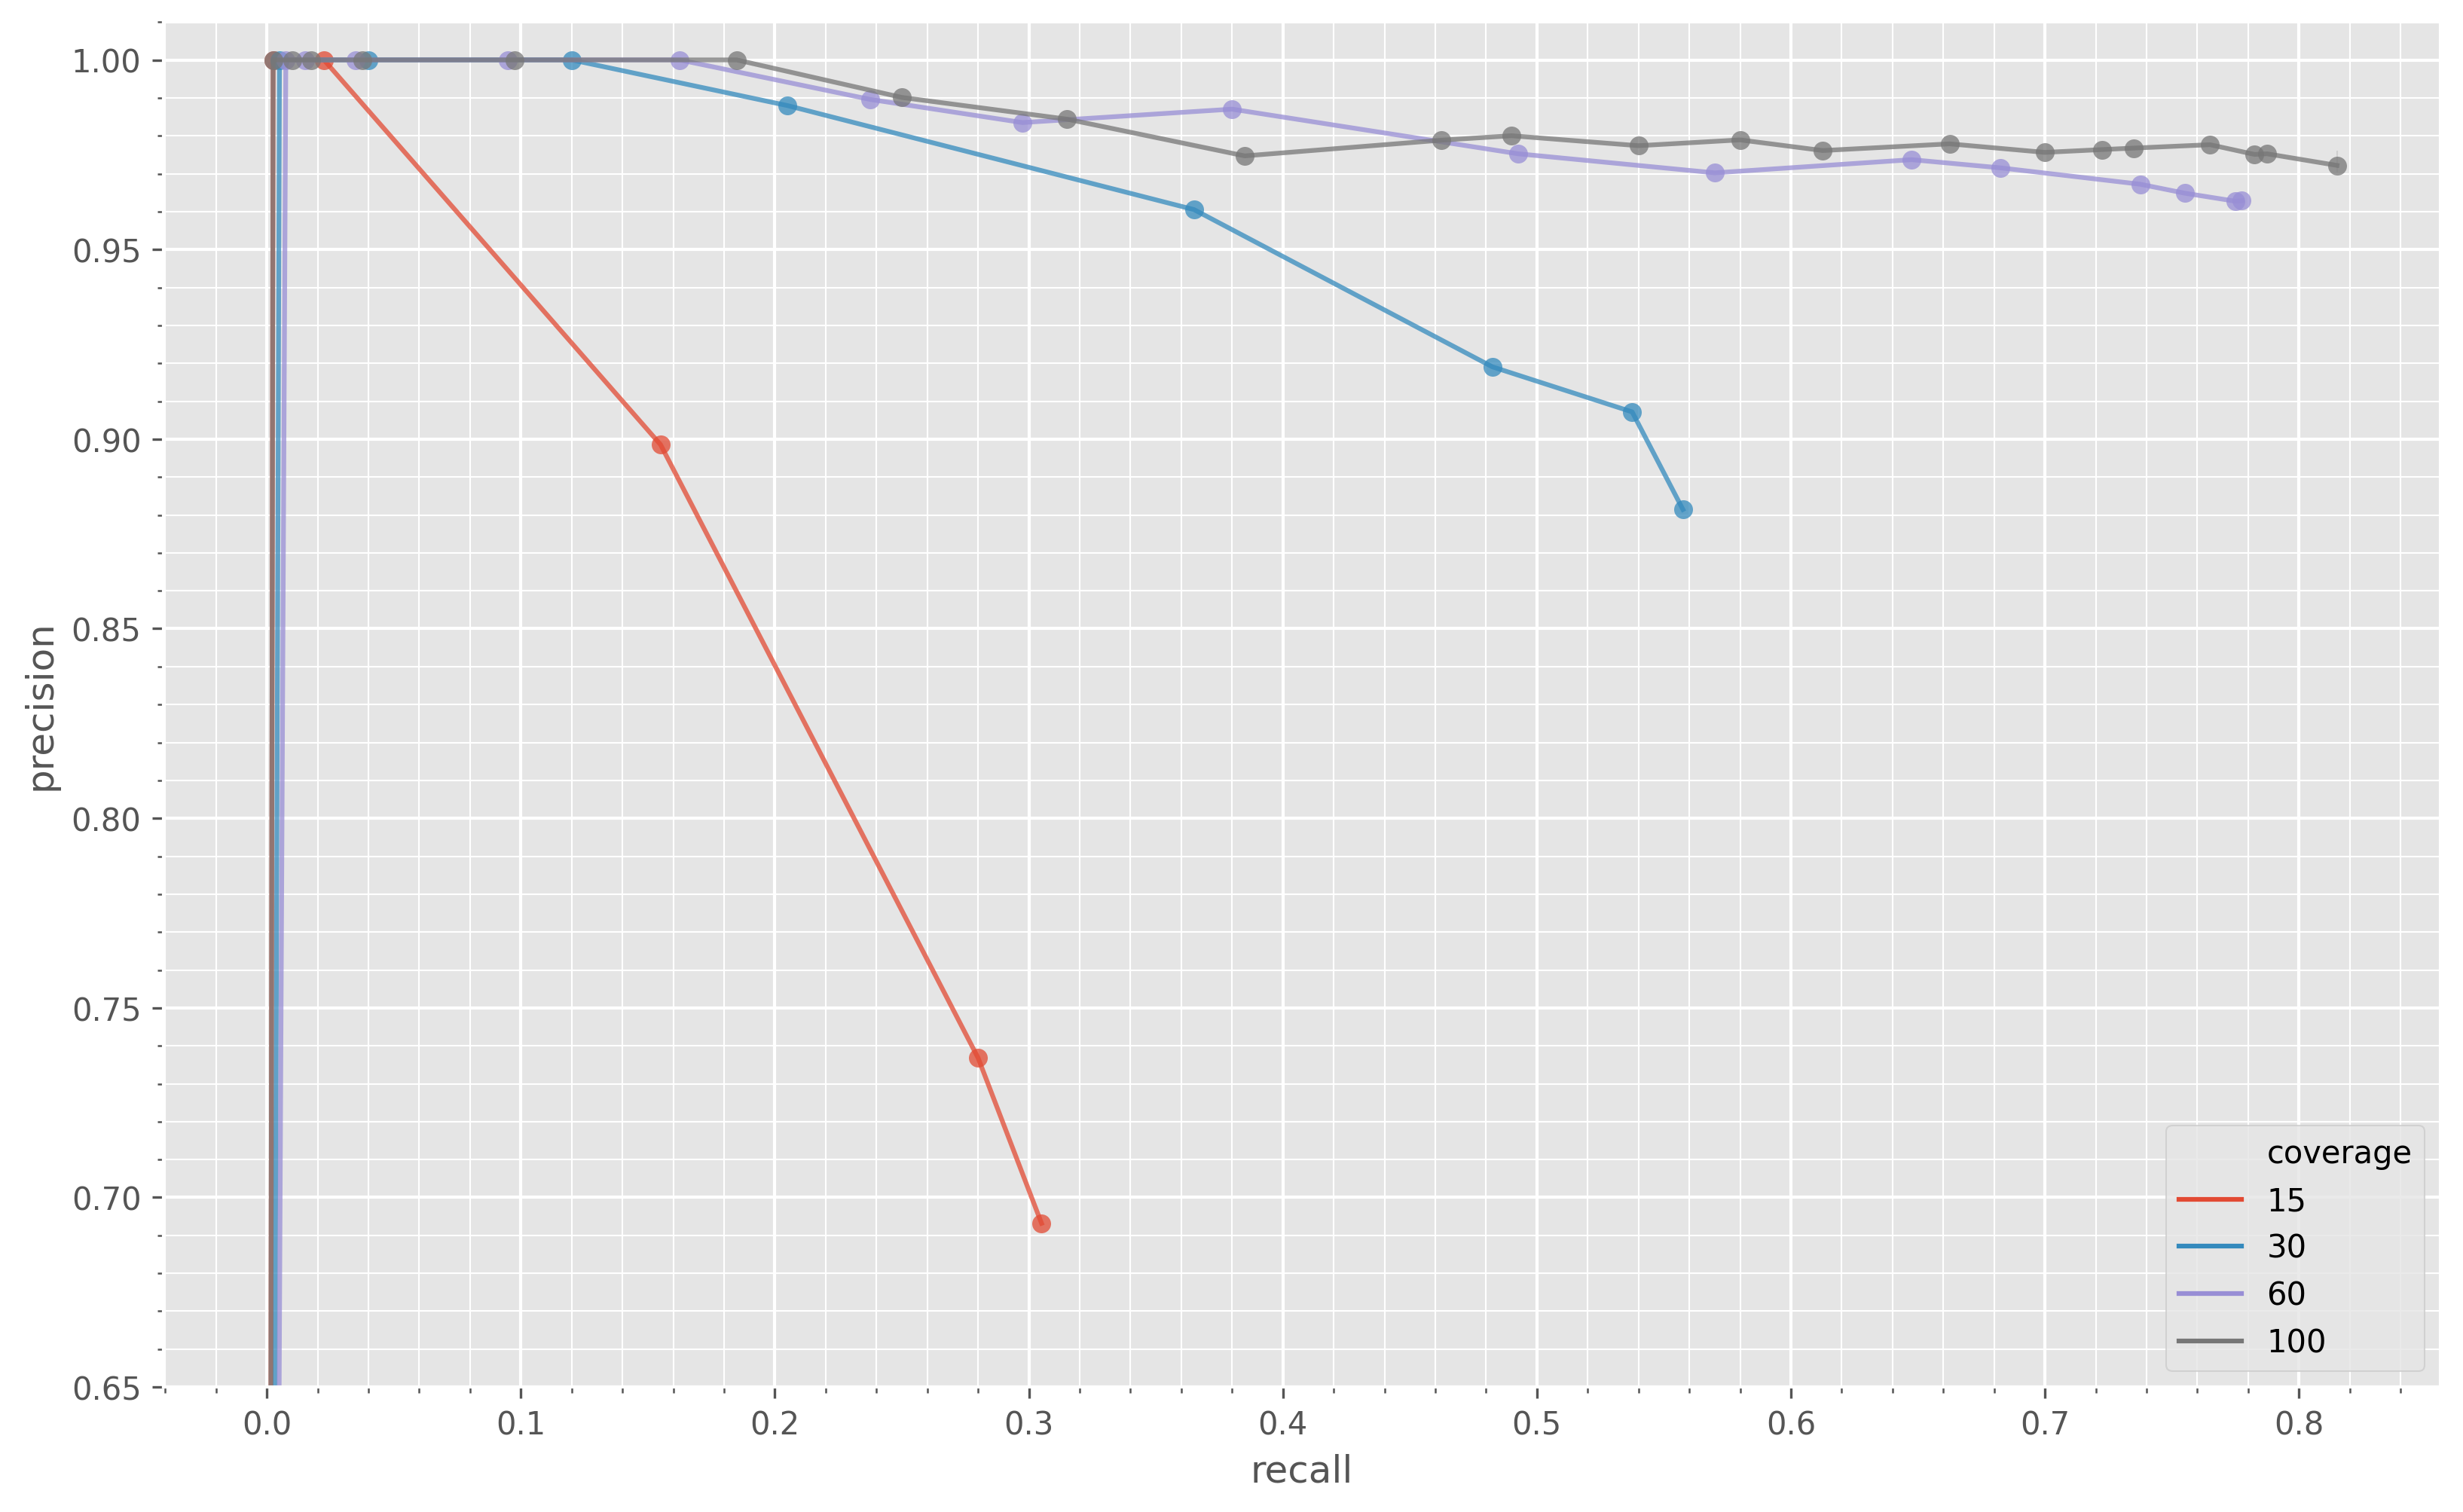
\includegraphics[width=0.9\textwidth]{Chapter1/Figs/denovo-sims-roc.png}
    \caption{Precision-recall curve for increasing genotype confidence score thresholds. The curves are coloured by read depth (coverage). Each marker/point is a different genotype confidence threshold, starting with 0 as the right-most value and increasing as the line moves towards the (top) left. Note, the y-axis has been cut to provide more clarity of precision.}
    \label{fig:denovo-sims-roc}
\end{figure}

\subsection{Summary}

In summary, we have shown that the addition of the \denovo{} variant discovery method outlined in \autoref{sec:denovo-method} gives \pandora{} the ability to find many variants not present in its \panrg{}. Using simulated data, we find a \kmer{} size of 13 gives slightly better recall than 11 or 15, but that the sample read depth has the most considerable impact on our ability to discover novel variants.

We have also shown that, on average, approximately 10.5\% of (simulated) SNPs are not detectable based on their membership in either loci \pandora{} does not detect, or lying within $2k-1$ positions of the start or end of a locus.

% ==================================================================
\section{Validation with empirical data}
\label{sec:denovo-empirical}

Having shown, for simulated data, that the \denovo{} variant discovery method indeed alleviates a major limitation of \pandora{}, we turn our attention to evaluating its performance on empirical data. However, rather than the single-sample (\pandora{} \vrb{map}) approach we used for genotyping in \autoref{sec:denovo-sims}, we evaluate \pandora{}'s multi-sample comparison protocol - \compare{}.

The inference of variation within a collection of samples is one of the unique aspects of \pandora{}. As detailed in \autoref{sec:pandora-compare}, the \vrb{compare} routine of \pandora{} genotypes multiple samples against a \panrg{} simultaneously, with the aim of representing variation between the samples in the most succinct manner possible (see \autoref{fig:var-representation}). It does this by selecting a single maximum likelihood path that best approximates the samples under investigation - akin to an "average" path of the samples.

Evaluating the variant calls from such a graph-based method is by no means trivial. In this section, we aim to compare the variant calls made by \pandora{} against those made by single-reference (linear) methods for both Illumina and \ont{} data.

In keeping with the focus of this chapter, we will also assess the utility of \denovo{} variant discovery within \pandora{}. While we have shown its benefit on simulated data, the \panrg{} used did not contain many of the simulated SNPs. However, we expect many of the SNPs in real data also to be present in a \panrg{} built from a pan-genome of diverse samples. 

\textit{Note: all work in this section (\autoref{sec:denovo-empirical}) is described in full in \cite{pandora}. See \autoref{sec:denovo-acknowledge} for a detailed description of what work was completed by myself.}

\subsection{Dataset}
\label{sec:denovo-empirical-data}

\subsubsection{Samples}
The empirical data we use for this evaluation is a diverse set of 20 \ecoli{} samples from four different phylogroups. Each sample has both \ont{} and Illumina sequencing data and high-quality assemblies available. The sequencing reads for each technology were subsampled to read depth 100x.

\subsubsection{References}
The \panrg{} we use as the reference for \pandora{} was constructed from a combination of \ecoli{} genes and intergenic regions. 23,054 gene MSAs from 350 RefSeq genomes were obtained from the panX database \cite{panx}, while 14,374 intergenic region MSAs from 228 ST131 genomes were collected from \cite{thorpe2018}. \prg{}s were constructed for each locus using \makeprg{} and then all were combined into a single \panrg{} file and indexed with \pandora{}.

As single-reference variant callers cannot use a \panrg{}, we selected 24 reference genomes from five major phylogroups - one phylogroup is not contained within the sample set. These references were selected to be spread across phylogroups, and where the phylogroup was present in our samples, we chose the nearest RefSeq genome according to Mash, and a phylogenetic tree \cite{pandora}. By calling variants for each sample with respect to each reference genome, we can directly view the impact of reference selection on the results of standard variant callers.

\subsection{Variant calling}

\subsubsection{Graph-based: Pandora}
To produce a multi-sample VCF file of variants for \pandora{} we follow a somewhat similar approach to \autoref{sec:denovo-sims-methods}, with some important differences. Rather than adding all \denovo{} variants for a single sample to the original \panrg{} we instead add the novel variants for \emph{all} samples to the original \panrg{}. In the end, we have an updated \panrg{} which contains all novel variants for all samples under comparison. We then perform multi-sample genotyping with this updated \panrg{} using \compare{}. This entire process is completed separately for Illumina and \ont{} data.

\subsubsection{Linear-based}
We compare the Illumina variant calls from \pandora{} against those from SAMtools \cite{samtools2009} and Snippy (\url{https://github.com/tseemann/snippy}) (which is a wrapper around Freebayes \cite{Garrison2012}). The \ont{} variant callers we evaluate against are Medaka (\url{https://github.com/nanoporetech/medaka}) and Nanopolish \cite{Loman2015}. Each variant caller is run on all 20 samples with all 24 reference genomes. 

\noindent
In total, we produce 480 VCFs for each linear variant caller and one multi-sample VCF for \pandora{}.

\subsection{Evaluation}
\label{sec:denovo-empirical-eval}

A direct comparison of the VCF files produced by \pandora{} and the single-reference tools is not possible due to coordinate incompatibilities. As such, we use a probe-based method, akin to that in \autoref{sec:denovo-sims-eval} for assessing the variant calls. 

The first step in this evaluation is the generation of a pan-genome SNP truth set. \autoref{app:pangenome-snp-truth} details the construction of this truth set, resulting in 618,305 SNPs we expect to find amongst the 20 samples.

There are two measures of recall in a pan-genome (see \autoref{app:pangenome-snp-truth}), but of interest to this section is the average allelic recall (AvgAR). Briefly, AvgAR is the average recall of all pan-genome variants. For example, we have three genomes with two pan-genome variants $P_1$ and $P_2$ between them. $P_1$ has the alleles A, A, and T across the three genomes, and $P_2$ has alleles C, T, and T. If we find the $P_1$ alleles A (for only one sample) and T, we have a $P_1$ recall of 0.66 (2/3), and if we only find the $P_2$ allele C, we have a $P_2$ recall of 0.33 (1/3). Therefore, in this example, we have an AvgAR of $\frac{0.66+0.33}{2}=0.5$.

To calculate AvgAR (recall) for tool-reference pairs, we perform the following: i) apply the variant calls for each sample to the reference sequence the calls were made with respect to (giving 20 mutated sequences); ii) we map all truth set probes to these mutated reference sequences with \vrb{bwa mem}; iii) we classify a mapping as TP if the alleles within the aligned sequences match. Then, for each pan-genome variant, we count the proportion of its alleles with a TP mapping and calculate AvgAR accordingly. In the end, we have an AvgAR value for each variant caller and reference sequence combination - i.e., 24 AvgAR values for each linear caller, and one value for \pandora{}.

We determine precision in a somewhat similar manner. First, we create probes for each variant in a given VCF, with 150bp of flanking sequence taken from the VCF reference sequence. Second, we map each probe to the sample's assembly sequence. Next, we filter out poor quality mappings or mappings to low-quality regions of the assembly. Finally, each mapping's precision is classified as a continuous score - rather than a binary true or false positive - by dividing the number of matching bases (ignoring the flanking sequences) by the alignment length. Thus, for example, if the called allele is ATG and maps to a sequence ATTG, the precision score is 0.75. Ultimately, we calculate precision as the sum of precision scores, divided by the number of evaluated calls.

\subsection{Effect of different \ont{} basecalling models}
\label{sec:denovo-methylation}

Previous work from Wick \etal{} has shown that for Enterobacteriaceae, the majority of \ont{} sequencing errors are related to Dcm methylation sites \cite{wick2019}. In version 3.2.1 of \guppy{} (the ONT-provided basecalling software) a new \emph{methylation-aware} model was made available. However, this new model is considerably slower to basecall reads than the default model. As \ecoli{} is a member of this family, we set out to test a subset of 4 samples from our dataset to see whether a methylation-aware model indeed has a noticeable impact on the precision and recall from \pandora{} - with and without \denovo{} variant discovery.

We basecalled the raw data for four samples from our dataset with both the default and methylation-aware models from \guppy{} version 3.4.5. Precision and recall (AvgAR) are calculated as per \autoref{sec:denovo-empirical-eval} and presented in \autoref{fig:denovo-methylation}. 

The precision-recall curves represent increasing genotype confidence filtering; the top-right of each curve is no filtering, and as the genotype confidence requirement is gradually increased, we reduce the error rate (increase precision) at the loss of recall. 

Two crucial observations from \autoref{fig:denovo-methylation} are that the use of a methylation-aware model increases both precision \emph{and} recall, and the use of \denovo{} discovery increases recall at the cost of precision. 

\autoref{tab:denovo-methylation} shows the precision and recall values for the unfiltered results (i.e., the top-right of each curve in \autoref{fig:denovo-methylation}). From this, we see that without \denovo{} variant discovery, using a methylation-aware model would allow us to recover 894.7 variants in 1000 - 3.3 more than with the default model; likewise, we would expect to make 0.5 errors per 1000 variants. Using \denovo{} variant discovery, the methylation-aware model allows us to discover 906.3 variants in 1000 - 4.8 more than the default model and 11.6 more than methylation-aware without \denovo{} discovery. In terms of errors, using a methylation-aware model leads to 3.7 less errors per 1000 variants with novel variant discovery enabled; however, it makes 0.41 more errors per 1000 variants than without novel variant discovery. 

\begin{figure}
    \centering
    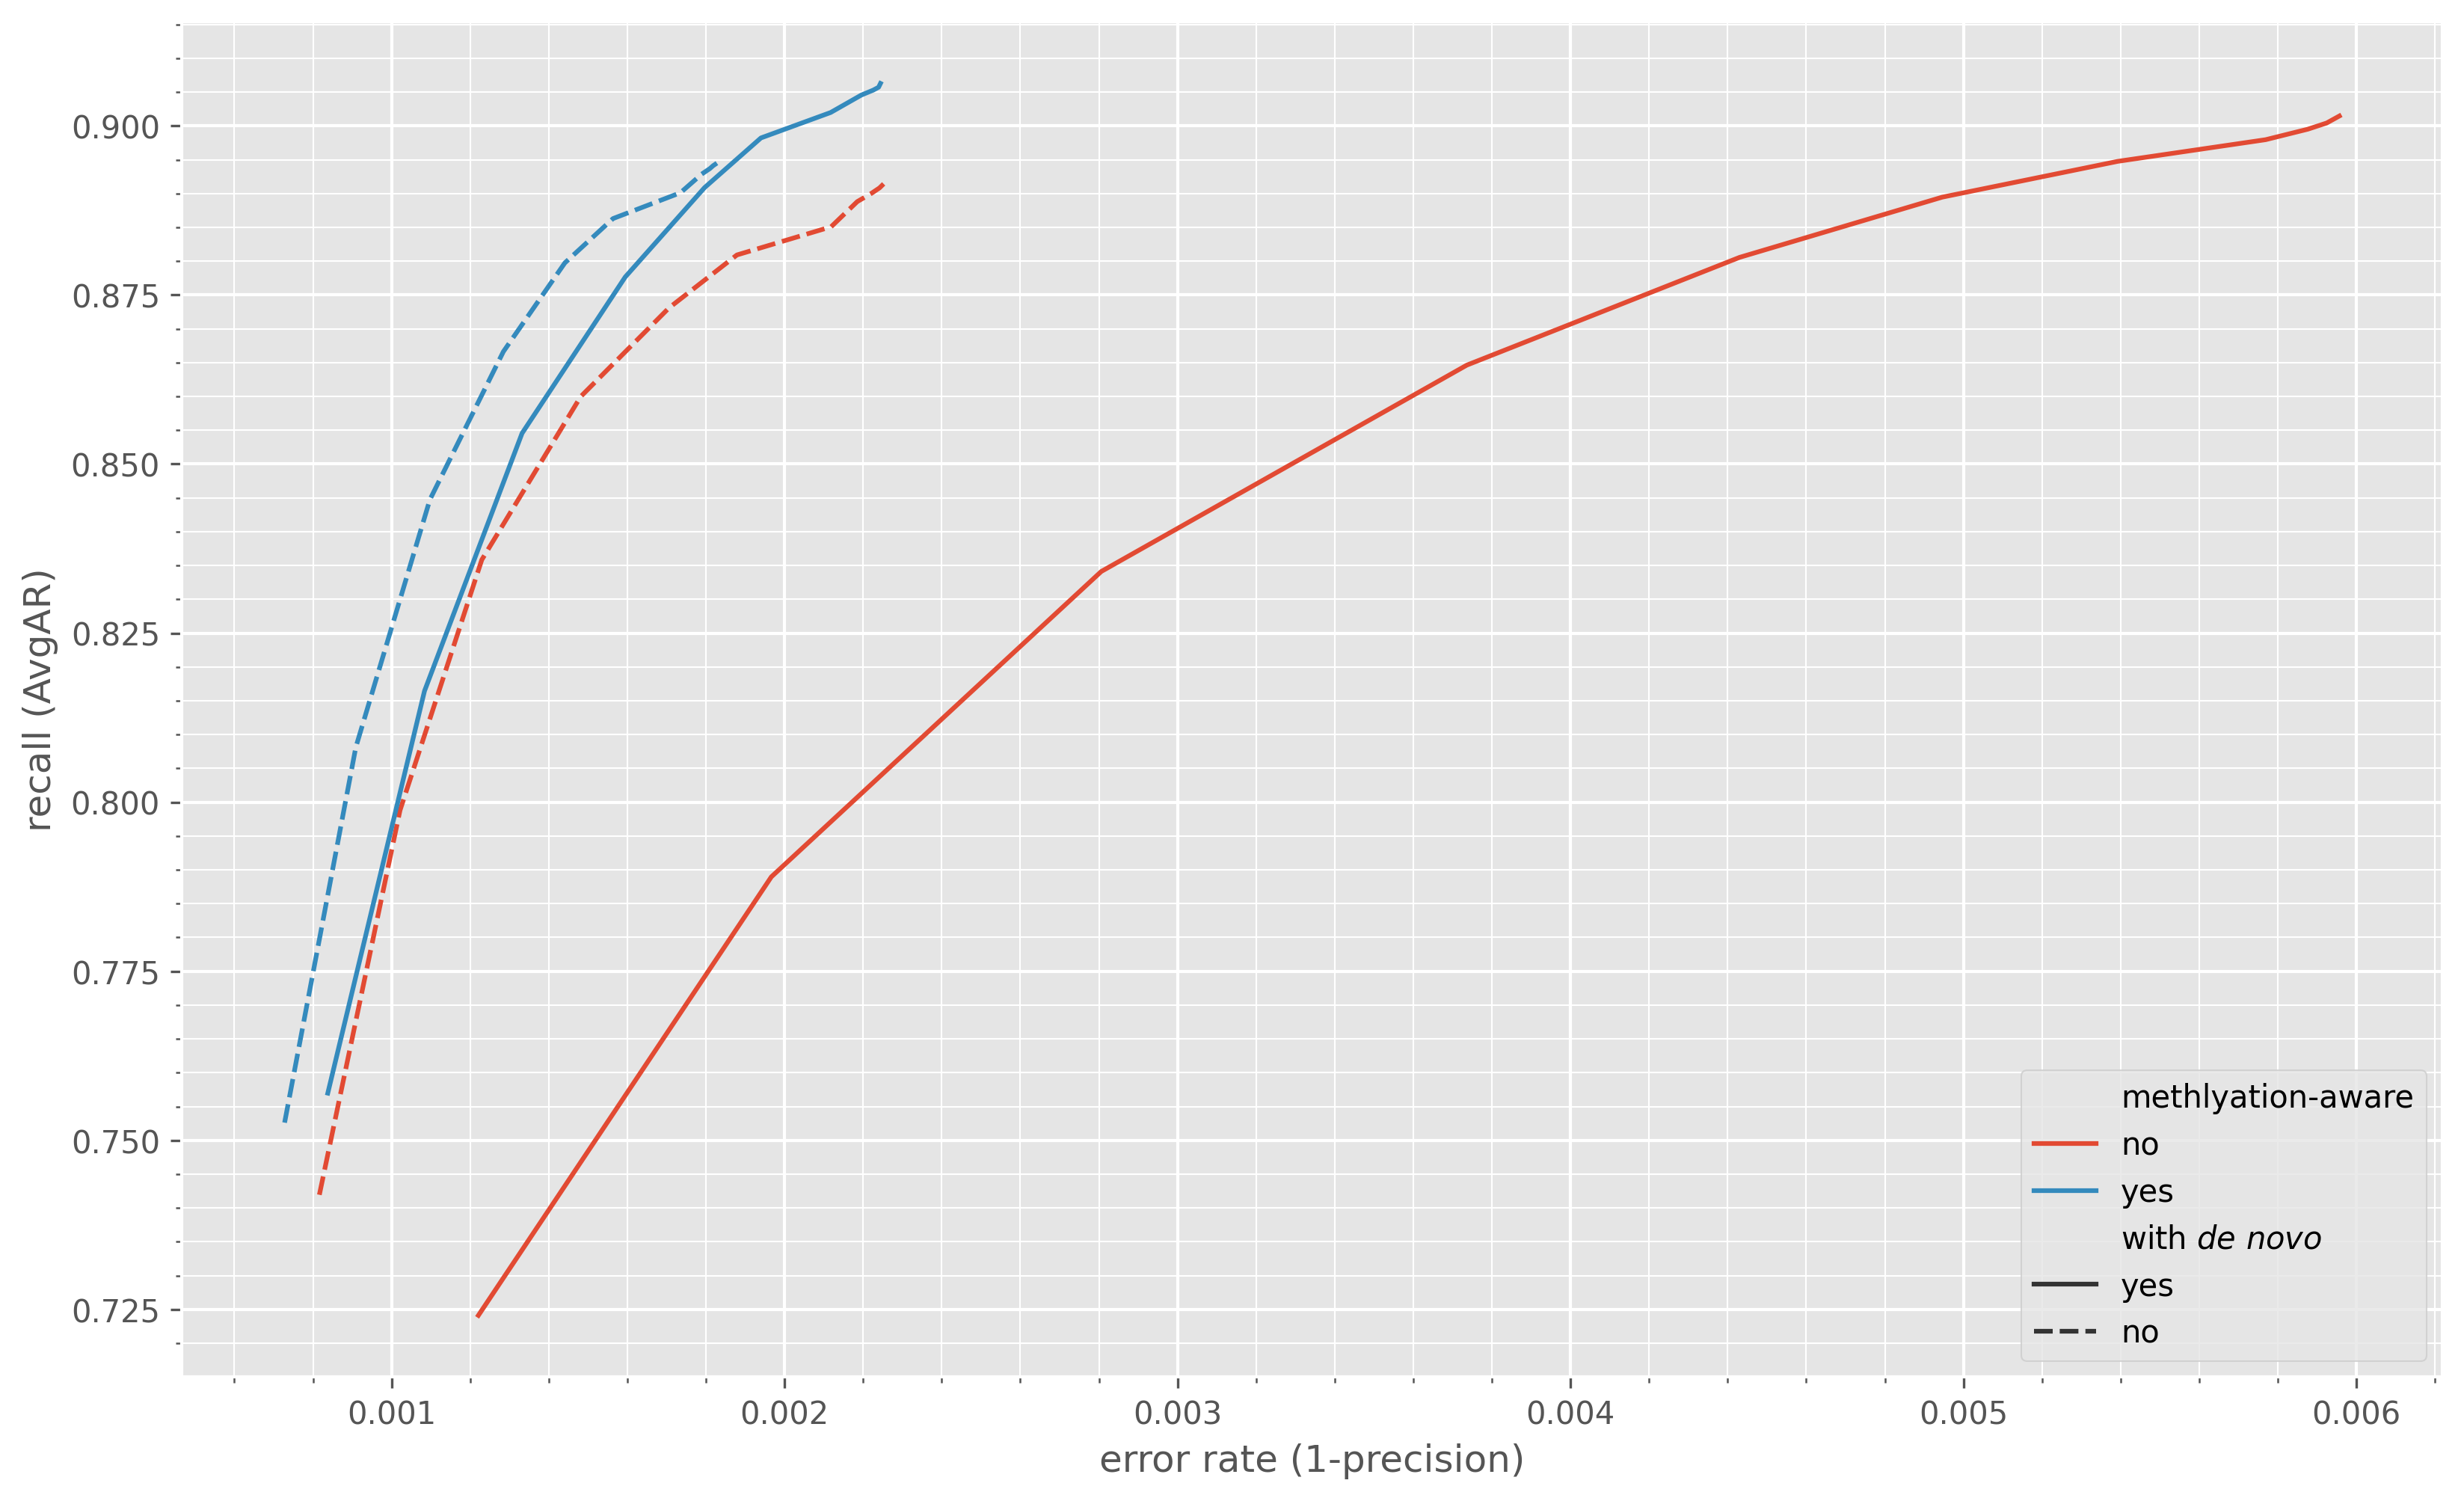
\includegraphics[width=0.9\textwidth]{Chapter1/Figs/pandora_basecaller_roc.png}
    \caption{Effect of \ont{} methylation-aware basecalling on \pandora{} \denovo{} variant discovery. The lines show the average allelic recall (AvgAR; y-axis) and error rate ($1-$precision; x-axis) of \pandora{} with increasing genotype confidence score thresholds with (solid line) and without (dashed line) \denovo{} variant discovery. The red line shows data basecalled with the default \guppy{} model and blue being basecalled with a methylation-aware model.}
    \label{fig:denovo-methylation}
    \source{Adapted from \cite{pandora} under the terms of the \href{https://creativecommons.org/licenses/}{Creative Commons CC BY license}. The colour scheme has been altered, along with the wording of some labels. However, none of these changes in any way alters the underlying data or interpretation of that data.}
\end{figure}

\begin{table}
\centering
\begin{tabular}{@{}llrr@{}}
\toprule
    Methylation-aware    & with \denovo{} & Recall (AvgAR)  & Error rate ($1-$precision) \\ \midrule
\multirow{2}{*}{no}  & yes                   & 0.9015          & 0.0060                   \\
                     & no                    & 0.8914          & 0.0023                   \\
\multirow{2}{*}{yes} & yes                   & \textbf{0.9063} & 0.0022                   \\
                     & no                    & 0.8947          & \textbf{0.0018}          \\ \cmidrule(l){2-4} 
\end{tabular}
    \caption{Effect of \ont{} methylation-aware basecalling on \pandora{} \denovo{} variant discovery (unfiltered) error rate ($1-$precision) and average allelic recall (AvgAR).}
\label{tab:denovo-methylation}
\end{table}

\noindent
Given the dramatic improvement in precision and recall from using the methylation-aware basecalling model, we re-basecalled all data for subsequent analyses with this model.

\subsection{Performance of Pandora against single-reference tools}
\label{sec:pandora-roc-results}

We now compare the precision and recall of \pandora{} on Illumina and \ont{} data against two single-reference variant callers for each technology. For the \ont{} analysis, we use the reads basecalled with the methylation-aware model (\autoref{sec:denovo-methylation}). In addition, we run \pandora{} with and without \denovo{} variant discovery to see the impact of the work in this chapter.

We use AvgAR as the measure of recall (see \autoref{sec:denovo-empirical-eval}) and apply increasing genotype confidence thresholds to illustrate the precision-recall trade-off. 

The results of this analysis are shown in \autoref{fig:pandora-roc}. For both sequencing technologies, \pandora{} with \denovo{} variant discovery has the highest (unfiltered) recall of 85.82\% on Illumina data and 85.51\% on \ont{}. In terms of error rate, \vrb{snippy} had the lowest Illumina unfiltered value of 0.01\% (with reference CP010170.1), while \pandora{} without \denovo{} variant discovery had the lowest \ont{} unfiltered rate of 0.19\%. 

Of particular interest to the work in this chapter is the observation that, on Illumina data, \denovo{} variant discovery leads to greater recall and precision (see inset of \autoref{fig:pandora-roc-illumina}); however, on \ont{} data, \denovo{} discovery provides greater recall, but at the cost of lower precision (see inset of \autoref{fig:pandora-roc-ont}). This suggests that systematic errors in \ont{} create incorrect novel alleles, which are in turn deemed correct by genotyping.

The most striking result from this work, though, is the error rate of \pandora{} on \ont{} data, which is 12.9 times lower than \vrb{nanopolish} and 79 times lower than \vrb{medaka}. In real terms, this equates to 22 and 146 fewer errors per 1000 variants, respectively.

Equally impressive is the improvement in recall over \vrb{snippy} using \pandora{} with variant discovery on Illumina data, leading to 47/1000 more variants being discovered. However, this does come at the expense of a higher error rate than \vrb{snippy}.

\begin{figure}
     \begin{subfigure}[b]{0.475\textwidth}
        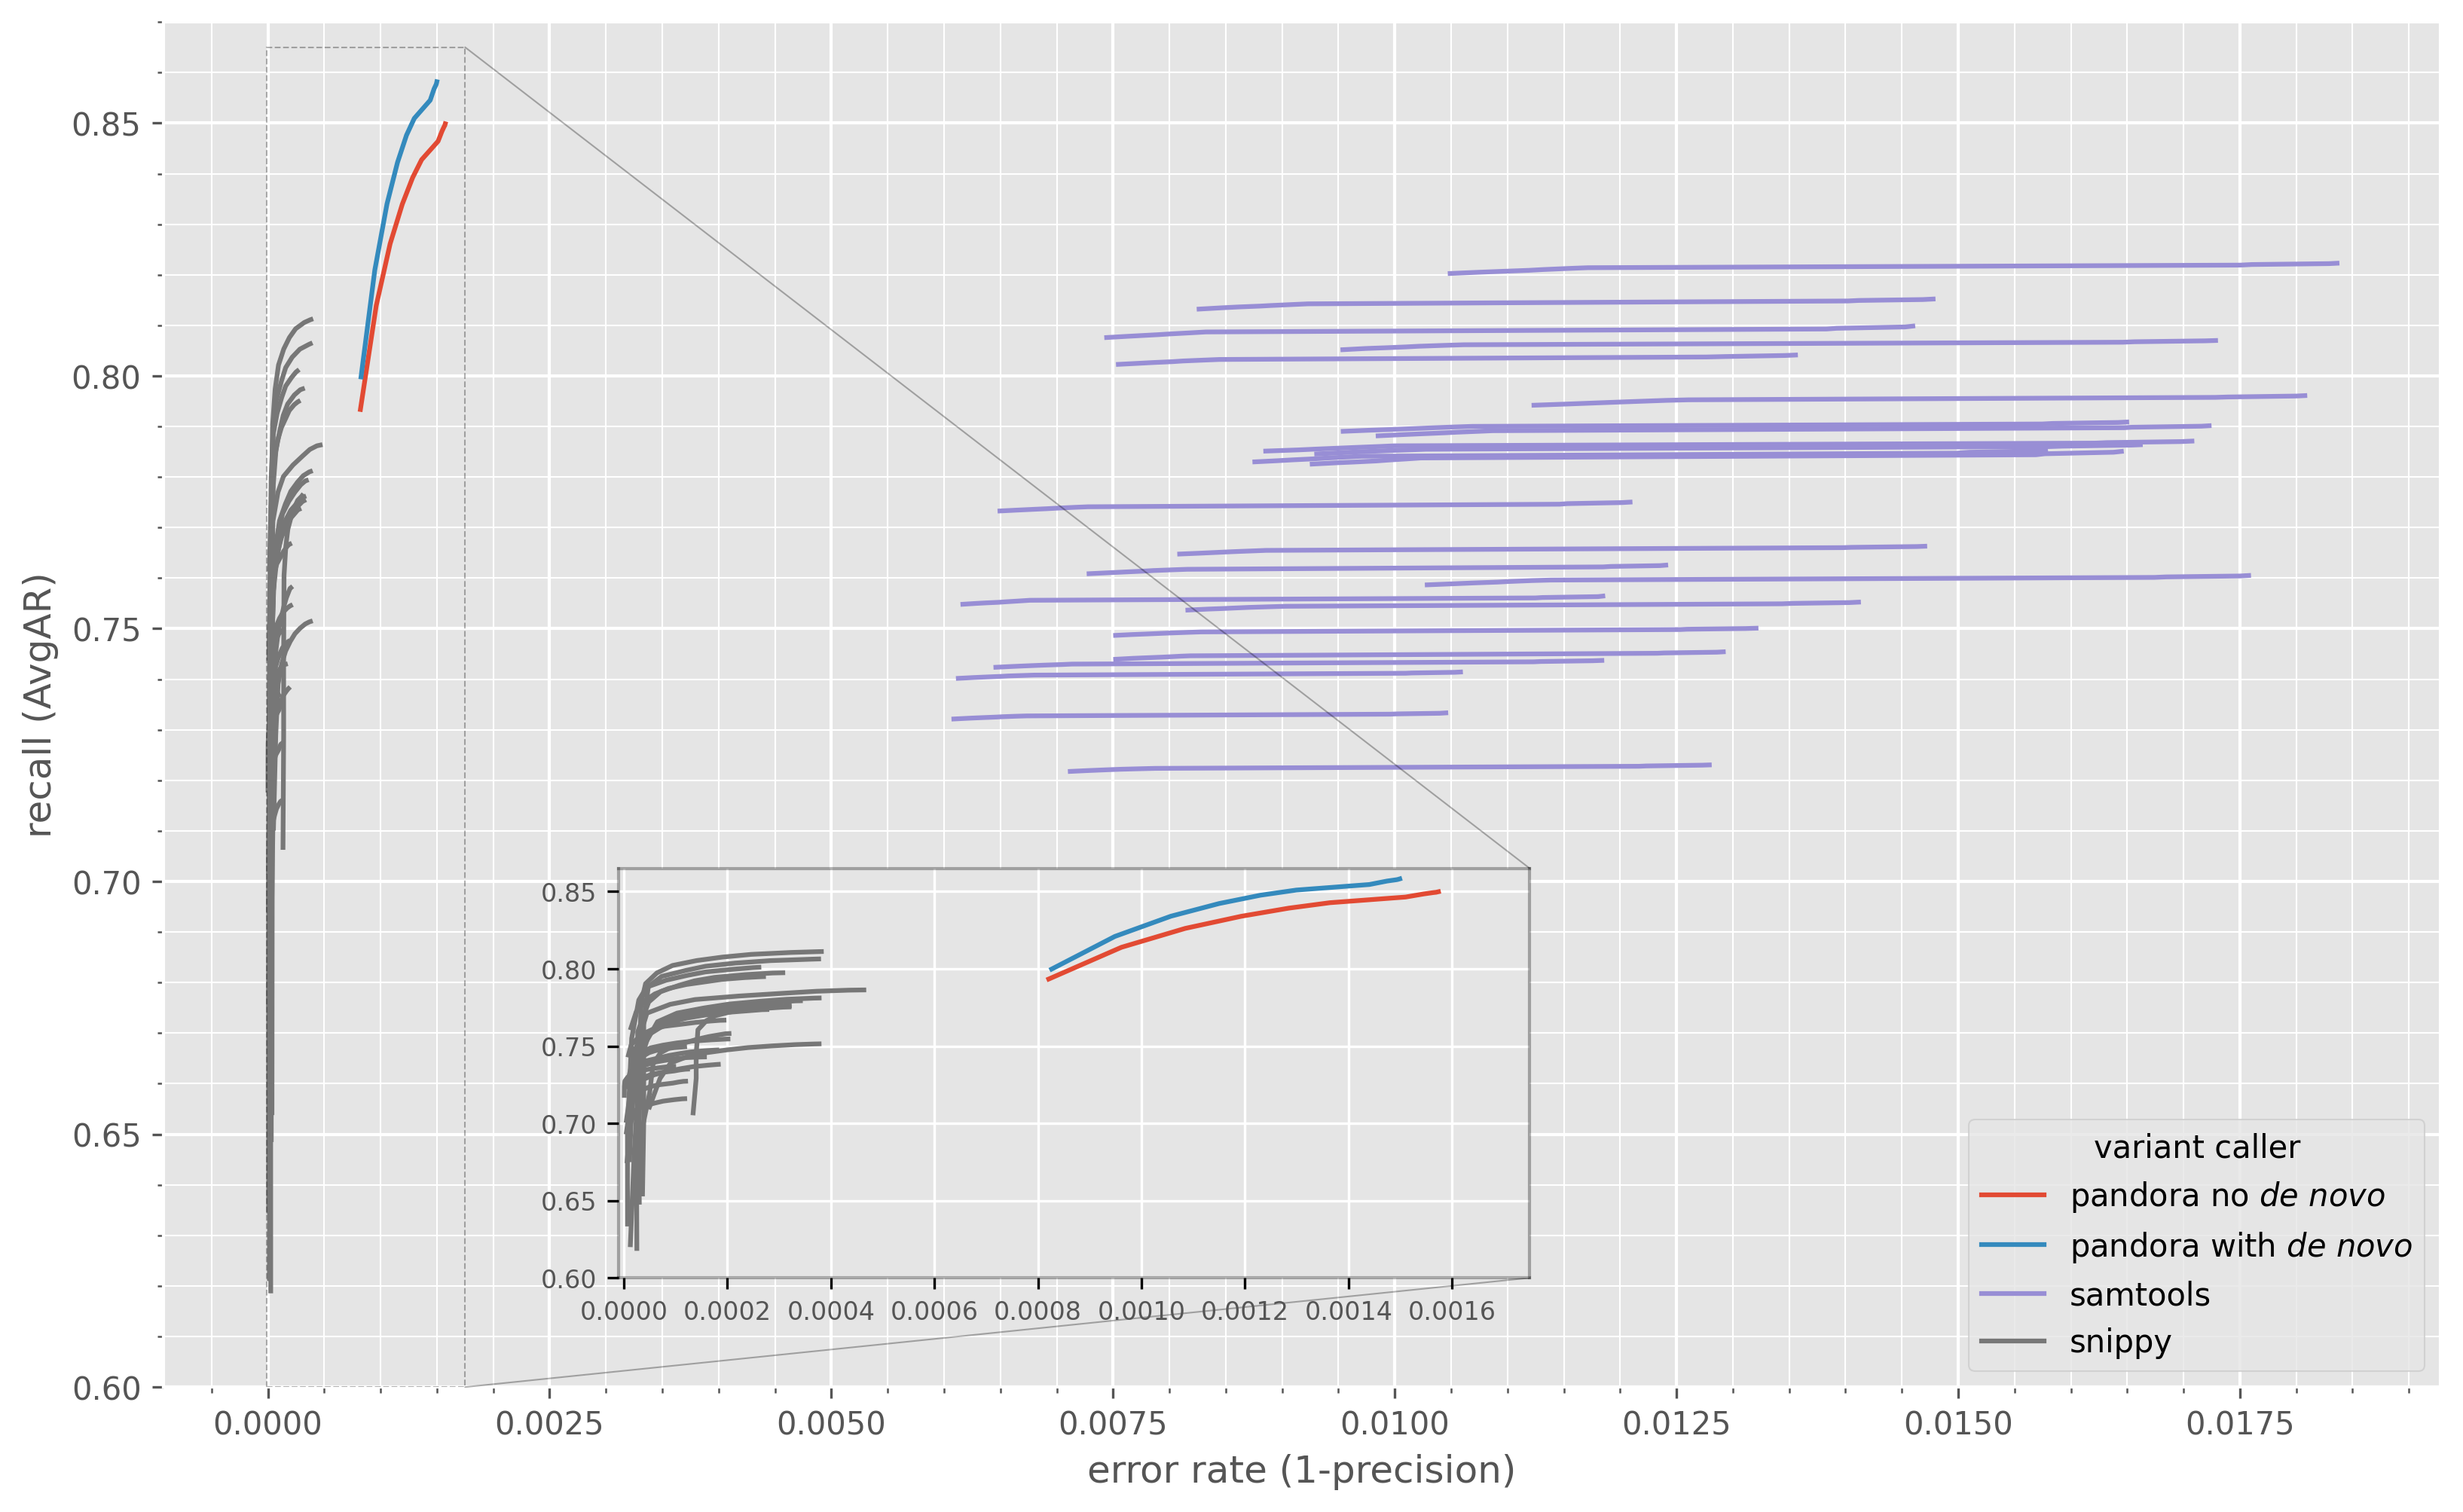
\includegraphics[width=1\linewidth]{Chapter1/Figs/illumina_roc.png}
        \centering
        \caption{Illumina}
        \label{fig:pandora-roc-illumina}
     \end{subfigure}
     \begin{subfigure}[b]{0.475\textwidth}
         \centering
        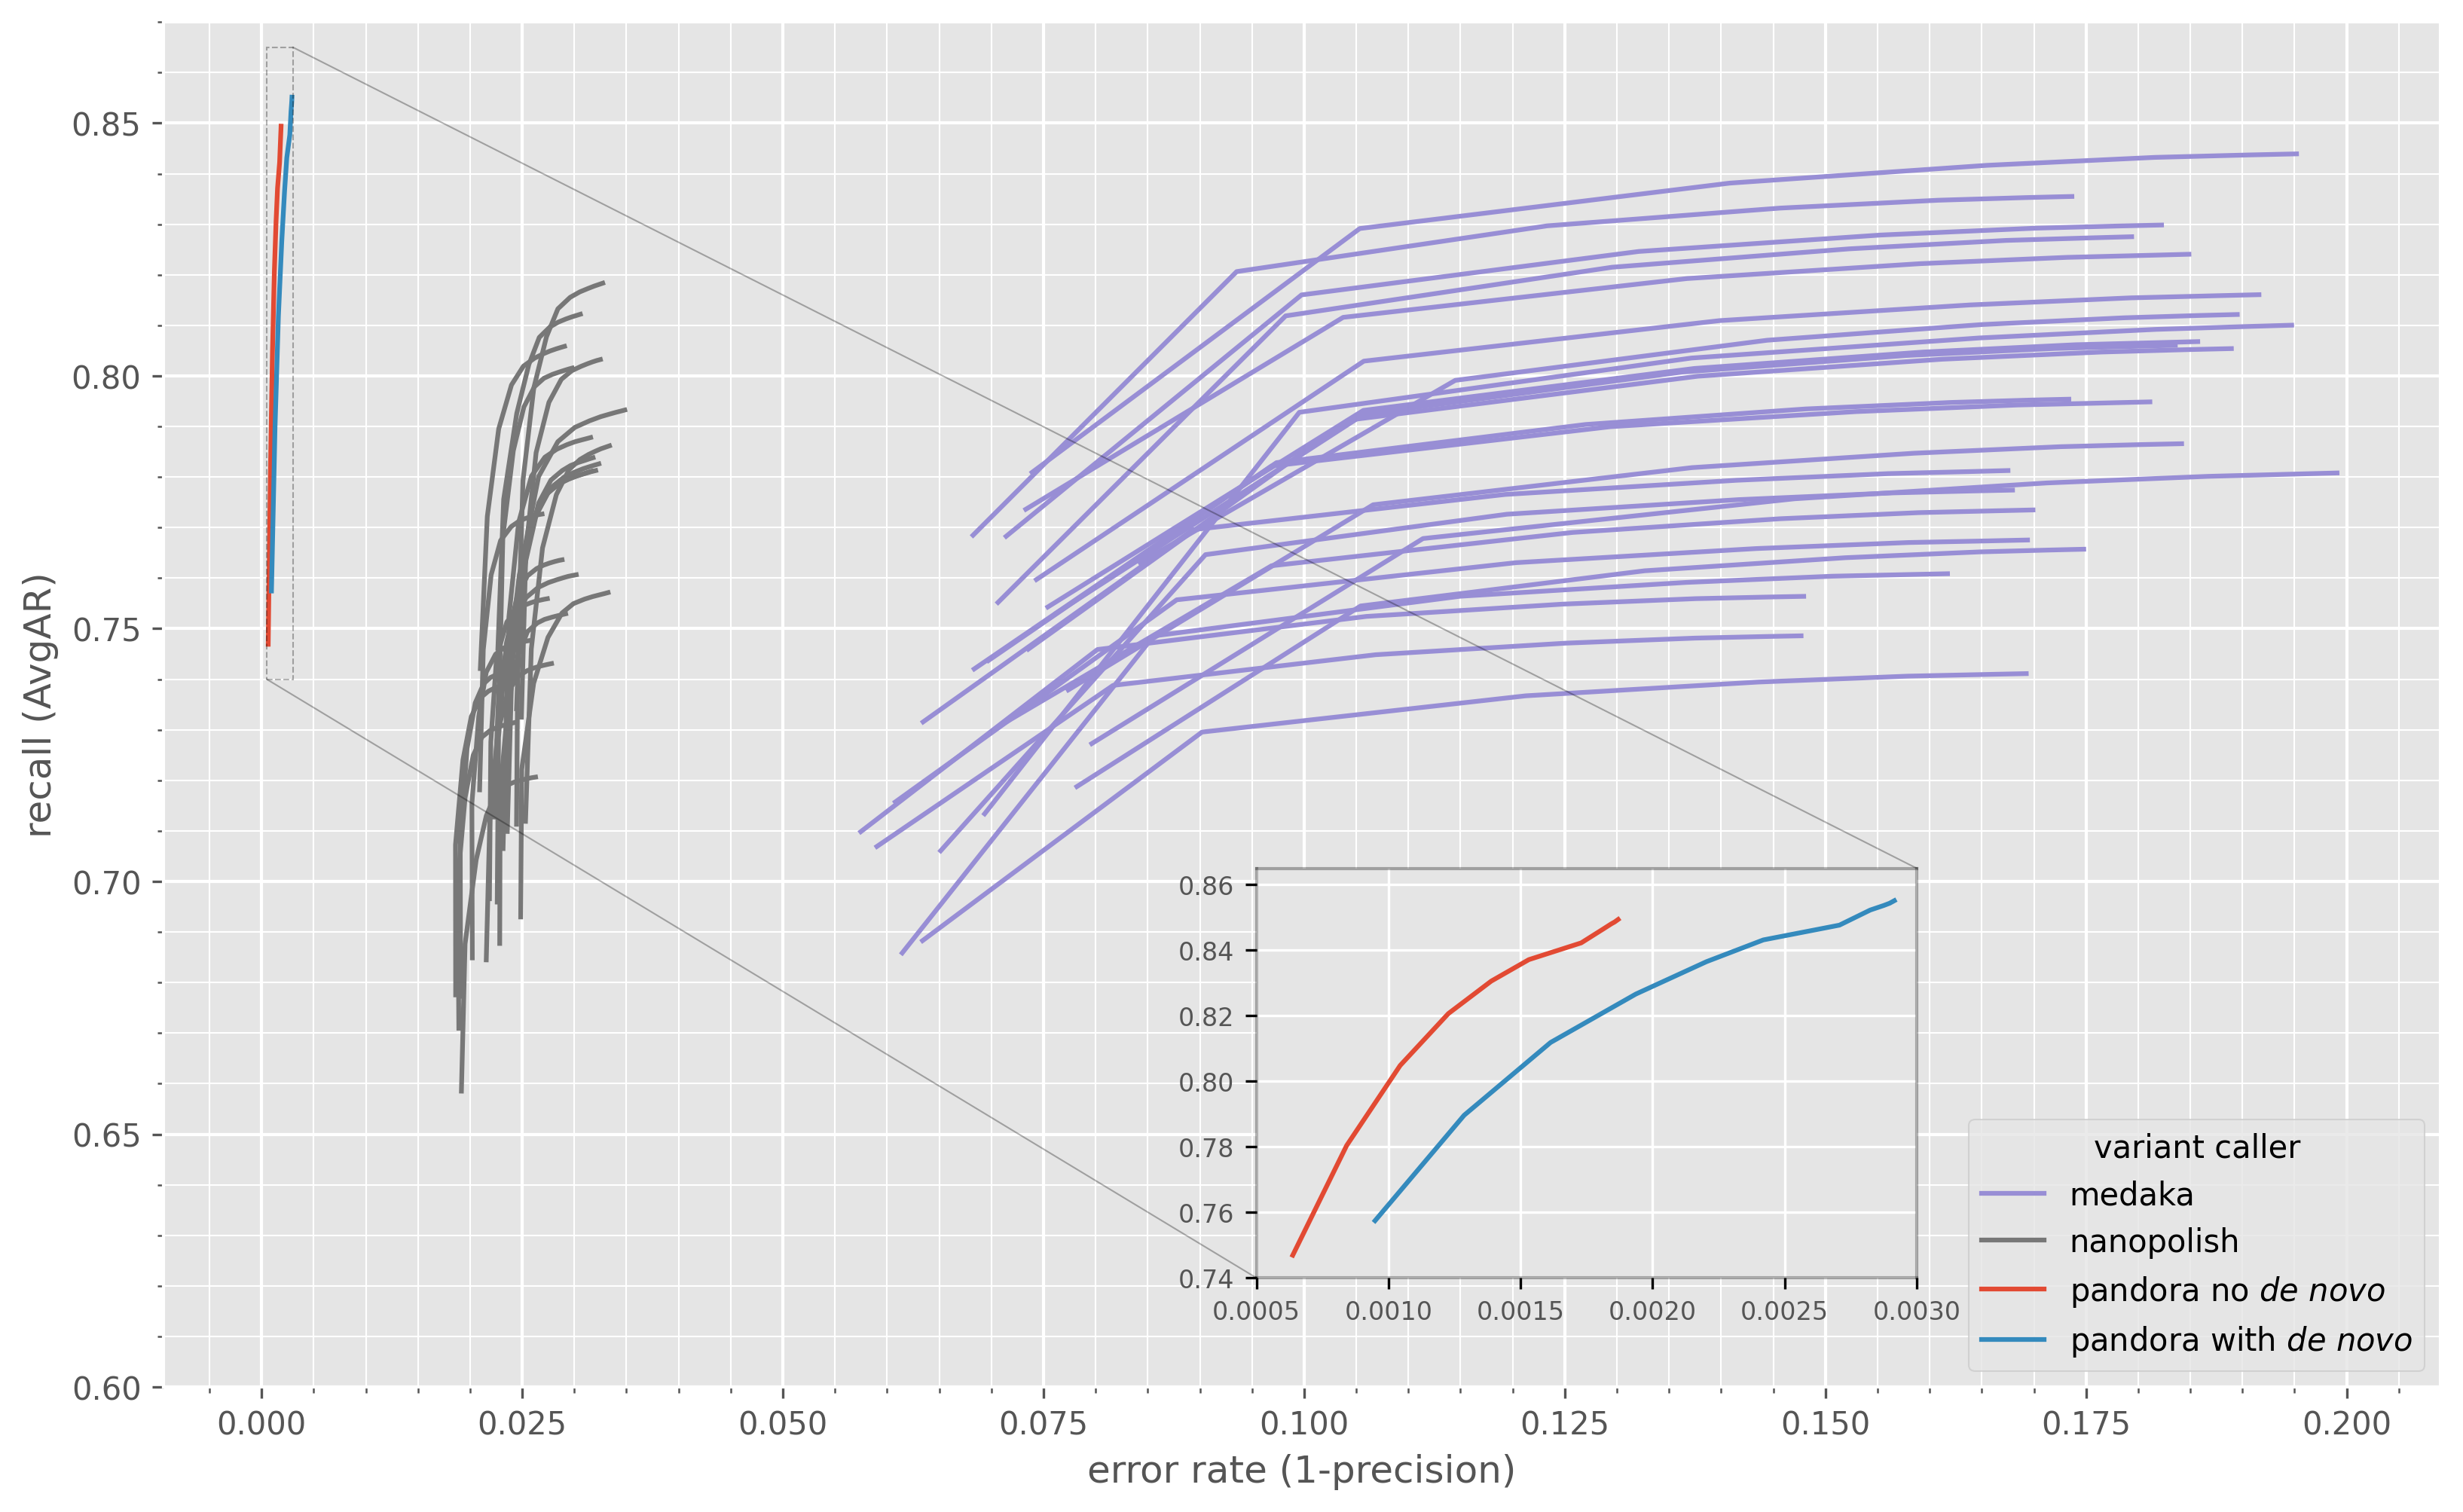
\includegraphics[width=1\linewidth]{Chapter1/Figs/nanopore_roc.png}
         \caption{\ont{}}
         \label{fig:pandora-roc-ont}
     \end{subfigure}
    \caption{Precision-recall curve for variant calls from Illumina (left; \textbf{(a)}) and \ont{} (right; \textbf{(b)}) data for different variant calling tools (colours). Each curve represents increasing genotype confidence thresholds, starting with no filtering in the top-right of each curve and increasing towards the bottom-left. \pandora{} has a single line with (blue) and without (red) \denovo{} variant discovery, which represents the error rate and recall across all 20 samples. The other variant callers are traditional single-reference tools; therefore, each line represents the use of 1/24 reference genomes from across five major \ecoli{} phylogroups. Inset windows are used to give more granularity for error rate in the best performing tools.}
        \label{fig:pandora-roc}
    \source{Adapted from \cite{pandora} under the terms of the \href{https://creativecommons.org/licenses/}{Creative Commons CC BY license}. The colour scheme has been altered, along with the wording of some labels, and the inclusion of inset windows. However, none of these changes in any way alters the underlying data or interpretation of that data.}
\end{figure}

\subsection{Summary}

In this section, using 20 diverse \ecoli{} samples, we have shown that the \denovo{} variant discovery method outlined in \autoref{sec:denovo-method} allows \pandora{} to discover more variants (increases recall). In addition, it improves the error rate on Illumina data.

We also demonstrated that a methylation-aware \ont{} basecalling model decreases the \pandora{} error rate - quite significantly for \denovo{} - indicating that many of the novel variants "discovered" by our method are, in fact, systematic technology errors.

Finally, we show that \pandora{} provides higher recall than single-reference-based variant callers for both Illumina and \ont{} data and leads to a \ont{} error rate that is an order of magnitude lower than other tools. However, \vrb{snippy} provides lower error rates than \pandora{} on Illumina data.

% ==================================================================
\section{Discussion}
\label{sec:denovo-discussion}

In this chapter, we described a method for discovering \denovo{} variation in a genome graph from both Illumina and \ont{} data. We implemented it in the \vrb{discover} subcommand of the reference graph program \pandora{} and evaluated its utility on both simulated and empirical data. Additionally, we demonstrate an approach for comparing variant calls made from single-reference or graph-based tools independent of genome coordinates.

Before the work in this chapter, \pandora{} was only able to genotype with respect to variation present in a pan-genome reference graph. To allow \pandora{} to discover novel variants, we use a localised form of genome assembly in segments of the graph with low \kmer{} coverage. We first identify candidate regions of the genome where read depth (observed as \kmer{} coverage) drops below a predefined threshold. Next, we slice out the segments of the reads that map to these candidate regions and construct a de Bruijn graph from them. Finally, we enumerate paths in this de Bruijn graph that pass coverage and insertion size filters and output them as novel candidate alleles. These alleles can then be added into the original \panrg{} to allow for genotyping against these new alleles.

This \denovo{} discovery process, detailed in \autoref{sec:denovo-method}, is somewhat analogous to the method used by GATK's HaplotypeCaller \cite{Poplin2018}. With two noticeable differences. First, GATK determines candidate regions (described as \emph{ActiveRegions}) based on an "activity score" that is calculated from alignment quality and genotype likelihood at a locus. In contrast, we use a naive approach that looks for \kmer{}s in the maximum likelihood path with coverage less than a hard threshold. While our approach may seem simple, it relies on information gained by performing quasi-mapping to the graph and inference of a maximum likelihood path. Second, the pruning methods employed by GATK involve removing edges with low support, and when the terminal \kmer{} of a path does not match the reference sequence, they attempt to use local alignment to merge it. By comparison, we require a path contain the terminal \kmer{}, thus avoiding local alignment. Additionally, we prune the de Bruijn graph by using depth- and breadth-first search to construct a distance map so that we know whether a given \kmer{} in the de Bruijn graph can reach the terminal \kmer{} within a predefined number of graph walks. In this way, we never get stuck in cycles or produce paths longer than a user-defined insertion size. 

While we did not compare \pandora{} runtime to GATK, given the results in \cite{Poplin2018} and the algorithmic details of their method, we suspect our method leads to much faster runtimes due to the pruning of paths and lack of local alignment.

\noindent
In \autoref{sec:denovo-sims} we selected random paths from a \panrg{} and randomly introduced SNPs to each at varying rates. We then simulated \ont{} reads from these mutated random genomes and used them to test different parameters relating to our \denovo{} discovery method. Read depth (coverage) had the most obvious impact on the ability to detect novel variants. Given the simulated \ont{} read error rate of approximately 11\%, the decrease in recall with coverage is expected as our method relies on \kmer{} coverage along the candidate paths. Without sufficient \kmer{} coverage to support a path, we cannot produce any candidate alleles. While a \kmer{} size of 13 for \denovo{} assembly was found to perform slightly better than 11 and 15, this was only marginal and may warrant further investigation. Indeed, for the work in \cite{pandora} we used a \denovo{} \kmer{} size of 15 in order to speed up variant discovery in some problematic loci.

While we compared the precision and recall of \pandora{} with and without variant discovery in the simulations, this was not a realistic scenario. However, these simulations were not intended to be entirely realistic (that was the purpose of \autoref{sec:denovo-empirical}). They were designed to illustrate the limitations of \pandora{} without the capacity to find novel variation and allow us to explore the impact of various parameters on variant discovery.  

\noindent
Given the contrived nature of the simulation analysis,  in \autoref{sec:denovo-empirical} we used an empirical dataset of 20 \ecoli{} samples from across four major phylogroups to examine the benefit of \denovo{} variant discovery. In performing this analysis, we devised a novel method for comparing variant-calling precision and recall across tools in a coordinate-agnostic manner. The main benefit of such an approach is the mitigation of hard reference bias, which occurs when the reference genome used for variant calling (or mapping) does not contain a locus (see \autoref{fig:reference-bias}). As the pan-genome of \ecoli{} is open, hard reference bias is a problem when comparing cohorts of diverse samples. Indeed, as shown in Figure 7 of \cite{pandora}, \pandora{}'s use of a locus-specific reference that is dynamically selected based on the cohort under study leads to tens of thousands more SNPs being discovered in rare loci (loci in 2-5 genomes) compared to single-reference variant callers.

An important finding from our empirical analysis is the impact of Enterobacteriaceae methylation on \pandora{}'s \ont{} error rate (\autoref{fig:denovo-methylation}). In particular, when using \denovo{} discovery, the \ont{} error rate is 3-fold lower when a methylation-aware basecalling model is utilised. This observation is also confirmed by Wick \etal{} in their work benchmarking \ont{} basecalling methods for Enterobacteriaceae \cite{wick2019}. They saw that the overwhelming error source was in Dcm methylation sites and that these errors could be virtually erased by training a taxon-specific basecalling model. It follows that given the dramatic decrease in \denovo{} errors as a result of using the methylation-aware model, these systematic biases are being captured and incorporated back into the \panrg{} by variant discovery. Therefore, any \ont{} work involving genomes subject to Dcm methylation would be wise to employ methylation-aware basecalling. Other tools such as \vrb{nanopolish} have incorporated error modelling to remove these systematic biases \cite{Loman2015}. However, as \ont{} sequencing evolves at a rapid pace, the constant maintenance required to model these errors can become very laborious. As such, we feel that taxon-specific basecalling models are a more robust solution to these systematic errors (we explore this further in \autoref{chap:tubby}).

Despite the impact of \ont{} systematic errors on \denovo{} variant discovery, we did find that for both Illumina and \ont{}, \denovo{} discovery increased the recall of \pandora{} (\autoref{fig:denovo-methylation} and \autoref{fig:pandora-roc}). In addition, we also found that \denovo{} discovery provided lower error rates on Illumina data (\autoref{fig:pandora-roc-illumina}). As the Illumina and \ont{} data for all samples are matched - i.e., from the same DNA extraction - the difference in error rate between \denovo{} and no-\denovo{} must be technology-driven. However, we do note that the \pandora{} error rate for \ont{} was an order of magnitude lower than both \vrb{medaka} and \vrb{nanopolish}.

\noindent
Without the addition of \denovo{} variant discovery, \pandora{}'s recall is higher than all other variant callers tested - although only marginally higher than \vrb{medaka}. This shows the power of genome graphs to provide access to sections of the genome previously unavailable to single-reference methods. Now that we have provided the functionality for \pandora{} to perform novel variant detection, the door is open to access even more of the pan-genome. 

One application that stands to benefit from pan-genome graphs is prospective surveillance of a bacterial population. Current approaches to such surveillance perform multiple levels of genome alignment in order to find the most appropriate reference for a given sample \cite{Gorrie2021}. In contrast, the \panrg{} used by \pandora{} is a stable reference capable of handling an evolving cohort.

% ==================================================================
\section{Limitations and future work}
\label{sec:denovo-limits}

\subsection{Path enumeration}
\label{sec:fw-path-enum}

A fundamental limitation of the \denovo{} variant discovery method outlined in this chapter is the need for anchor \kmer{}s to initiate local assembly and perform path enumeration. While this is not concerning in most locus areas, it becomes problematic near the start and ends of loci (within $2k-1$ positions of the ends). Indeed, we see in \autoref{fig:denovo-errors} that on simulated data, variants that occur near the ends of loci account for a recall loss of 8\%.

One solution for removing this anchor \kmer{} limitation would be to use a unique \kmer{} approach analogous to Kevlar \cite{Standage2019}. Briefly, Kevlar aims to detect \denovo{} variants (in human trios/families) by looking for unique \kmer{}s in a child, with respect to the parents. Reads containing these "interesting" \kmer{}s are then assembled with an overlap graph, and the resulting contig is aligned to and genotyped against the reference.

Our idea for how the Kevlar method could be adapted to \pandora{} is to identify candidate regions and extract the read pileups for these regions as we currently do (\autoref{sec:denovo-candidate-regions}). Then, for each candidate region, perform the following: i) let $M$ be the set of all minimizer \kmer{}s along the maximum likelihood path in the candidate region; ii) construct a \kmer{} count table from the read pileup of the candidate region, only counting minimizer \kmer{}s not in $M$; iii) filter out any \kmer{} with a count less than some threshold determined by the number of reads in the pileup, leaving a set of unique minimizer \kmer{}s $N$. We would then construct a de Bruijn graph from only those reads containing \kmer{}s in $N$. The enumeration of paths through this graph would then involve beginning from any one of the \kmer{}s in $N$ - removing the need for anchors - and only keeping those paths that contain a \kmer{} in $N$. One element of this strategy that requires careful thought is how to incorporate paths back into the graph without the anchor \kmer{}s we currently use.

\subsection{Cycle detection}
\label{sec:denovo-cycles}
The primary computational bottleneck we have encountered during \denovo{} variant discovery development is infinite cycles in the de Bruijn graph. As de Bruijn graphs are directed, but not necessarily acyclic, a cycle can occur when a \kmer{} (node) can reach itself by following a path from any of its successor (out) nodes. When multiple such cycles occur within a graph, computational performance suffers. Such cycles can be detected using depth-first search; however, we do not want to disallow them as cycles are not invalid biologically. 

To limit becoming stuck in cycles, we employ pruning heuristics (\autoref{sec:denovo-prune}) that prevent paths from reaching a maximum length or the exploration of paths that will never reach the end anchor \kmer{}. However, if many cycles occur in close succession, even these heuristics do not prevent bottlenecks. Moreover, in some low complexity \prg{}s, we have seen this process take on the order of days for a single candidate region. As such, future work to improve the computational performance would be well-served to investigate additional pruning strategies. 

\subsection{\ont{} homopolymer deletions}
Wick \etal{} found Dcm methylation sites to be the primary source of errors in Enterobacteriaceae, and when these were eliminated with their taxon-specific model, homopolymer deletions became the chief error source \cite{wick2019}. 

While we did not report the number of homopolymer deletions we found, we did discover one as the source of 1/9 false negatives in our best-performing parameter set in the simulations (\autoref{sec:denovo-sims-results}). As mentioned, some methods attempt to remove these errors as part of their model explicitly. One such possibility would be to refuse to perform \denovo{} discovery on candidate regions containing homopolymer sites. However, we feel such an approach is too coarse and explore a potential solution in \autoref{chap:tubby} that entails training a species-specific \ont{} basecalling model.  

\subsection{Inserting novel alleles into the \panrg{}}
\label{denovo-fw-insert}

In \autoref{sec:denovo-insert} we described a somewhat convoluted process for inserting candidate paths found by \denovo{} discovery into a \panrg{}. This insertion approach is another of the main computational bottlenecks we encountered due to the need to perform a multiple sequence alignment. 

Leandro Ishi has been working on a prototype version of \makeprg{} (\url{https://github.com/leoisl/make_prg}) that facilitates much faster insertion of novel variants into a \panrg{}. When building a \prg{}, it additionally produces a customised data structure that acts as a way of remembering how sequences were clustered and collapsed. In addition, a prototype version (0.9.0) of \pandora{} changes the way \denovo{} discovery produces candidate paths. Rather than outputting them as sequences flanked by the maximum likelihood path sequence, it describes them in a custom format similar to VCF, with the addition of information about the \prg{} site the novel variant occurs in. Leandro has then implemented a new routine within \makeprg{} - \vrb{update} - which takes these custom data structures and attempts to add the novel variants directly into the \prg{}, only requiring the relevant sites to be recalculated. 

\subsection{Insertions and deletions}

A limitation we regret is not including indels in the simulations (\autoref{sec:denovo-sims}). Evaluating indels can become quite complex, and we suspect fine-tuning our method to produce high-quality indel calls will require a lot of time and care. On the other hand, simulations are the ideal environment in which to begin this work, as gathering a truth set of indels for empirical data is notoriously tricky. Thus, future work will begin by including indels in these simulations and then moving to well-characterised indel models for empirical data such as \cite{Bush2021}.

% ==================================================================
\section{Availability of data and materials}

The \pandora{} software is available at \url{https://github.com/rmcolq/pandora} under an MIT license. The \denovo{} method described in this chapter is implement in the command \pandora{} \vrb{discover}.

The analysis pipeline for the simulations in \autoref{sec:denovo-sims} is available at \url{https://github.com/mbhall88/pandora_simulations}. The data used for the \panrg{} in these simulations was obtained from \url{https://pangenome.org/Escherichia_coli}. The \ont{} reads used in the simulations was downloaded from Nic Loman's blog post \url{http://lab.loman.net/2017/03/09/ultrareads-for-nanopore/}.

All data and materials for the empirical data analysis in \autoref{sec:denovo-empirical} is described in \cite{pandora} and the corresponding GitHub repository \url{https://github.com/iqbal-lab-org/paper_pandora2020_analyses}.
%!TEX root = ../thesis.tex
%*******************************************************************************
%****************************** Second Chapter *********************************
%*******************************************************************************

\chapter{\ont{} sequencing for \mtb{} transmission clustering}
\label{chap:clustering}

\ifpdf
    \graphicspath{{Chapter2/Figs/Raster/}{Chapter2/Figs/PDF/}{Chapter2/Figs/}}
\else
    \graphicspath{{Chapter2/Figs/Vector/}{Chapter2/Figs/}}
\fi


%%%%%%%%%%%%%%%%%%%%%%%%%%%%%%%%%%%%%%%%%%%%%%%%%%%%%%%%%%%%%%%%%%%%%%%%%%%%%%%%%
%%%%%%%%%%%%%%%%%%%%%%%%%%%%%%%%%%%%%%%%%%%%%%%%%%%%%%%%%%%%%%%%%%%%%%%%%%%%%%%%%
\setcounter{section}{-1}
\section{Publication and collaboration acknowledgements}
\label{sec:ch2-acknowledge}

A manuscript comprising the work in this chapter and \autoref{chap:dst} is currently being prepared. The only work that was not completed by myself is the DNA sequencing of the samples.
The DNA extractions, and Illumina and \ont{} sequencing for the samples from Madagascar were sequenced by Marie Sylvianne Rabodoarivelo and Simon Grandjean Lapierre. The PacBio sequencing for these samples was performed by the Next Generation Genomics Core within Cold Spring Harbor Laboratory.
\towrite[inline]{acknowledge the people who did the south african sequencing}
\towrite[inline]{acknowledge the people who did the birmingham sample sequencing}
The variant-calling of all Illumina samples was performed by Fan Yang-Turner at the Nuffield Department of Medicine, University of Oxford. 
While the bioinformatic work (except the Illumina variant-calling) in this chapter was done by myself, I must acknowledge the wonderful guidance I have received. My supervisor Zamin Iqbal who always knows the right questions to ask. Simon Grandjean Lapierre, who helped conceive of this study, along with Zam, and who's clinical perspective helped keep me grounded in the real world. I would also like to acknowledge the many insightful conversations with our other collaborators: Marie Sylvianne Rabodoarivelo, Anastasia Koch, Niaina Rakotosamimanana, Anzaan Dippenaar, and Helen Cox. And finally, Tim Peto, who's input helped shape some of the clustering evaluation.

%=========================================================================

\section{Introduction}
% ebola work https://www.ncbi.nlm.nih.gov/pmc/articles/PMC4734547/ and https://www.nature.com/articles/nature16996
% zika work https://genomemedicine.biomedcentral.com/articles/10.1186/s13073-016-0356-2
% SARS-CoV-2 https://www.sciencedirect.com/science/article/pii/S1473309920305624
\mtb{} is a contagious bacterial pathogen that causes the disease Tuberculosis (TB) and accounts for more deaths than any other pathogen each year. As such, detecting chains of \mtb{} transmission is of the utmost importance. Whole-genome sequencing (WGS) is establishing itself as a key tool for identifying possible transmission clusters and is being used by many leading public health agencies to aid contact-tracing. Illumina is considered the gold-standard for this type of WGS work. However, in many high-burden TB settings, Illumina is not readily available and requires considerable time and resources to start and maintain. \ont{} has shown itself to be adept in these types of settings, having been used to great effect during Zika and Ebola outbreaks. Even in environments where resource availability may not be a problem, \ont{}'s rapid turnaround time has been used for monitoring COVID-19 and informing infection control measures. The time and resources required to set up \ont{} sequencing are far lower than Illumina, but despite this, there has been little work done to assess its suitability for \mtb{} WGS-based transmission clustering. The lack of work in this space likely stems from the long-held belief that due to its higher sequencing error rate, \ont{} is not capable of such fine-grained analyses. However, \ont{} has seen considerable improvements in its accuracy in recent years and studies using variant calls from the technology are becoming increasingly common. In particular, Public Health England (PHE) has investigated the use of \ont{} for the analysis of Shiga toxin-producing \ecoli{} and found it to be well-suited to the application. \\
In this chapter, we evaluate whether \ont{} sequencing can provide \mtb{} transmission clusters consistent with Illumina. To facilitate this investigation, we collect a new dataset of 150 samples - from Madagascar, South Africa, and England - sequenced on both Illumina and \ont{} platforms. We first assess \ont{} variant calls and outline a filtering strategy to provide Illumina-level precision. We use these variant calls to cluster samples based on SNP (single nucleotide polymorphism) distance thresholds and find \ont{} does not miss any samples from their expected cluster. Finally, we show that reliable clustering can be performed on samples from a mixture of Illumina and \ont{} modalities. \\
\mtb{} has a "closed" pan-genome; most (but not all) gene content is shared by all species members. In \autoref{chap:denovo} we sought to improve variant calling of bacterial pan-genomes with genome graphs. The work in that chapter was performed on \ecoli{}, which has an "open" pan-genome. In the interest of understanding how such genome graph methods can aid in closed pan-genomes, we additionally assess transmission clusters produced from \pandora{} variant calls. We construct two \mtb{} reference graphs from different densities of population variation towards this end. While the clustering from \pandora{} does not quite perform to the standards of the single-reference caller bcftools, we gain many insights for the improvement of \pandora{} and the construction of genome graphs.

%=========================================================================

\section{Dataset}
\label{sec:dataset}

The data used for the work in this chapter, and \autoref{chap:dst}, are patient-derived \mtb{} isolates from culture. We gathered samples from Madagascar (118), South Africa (83), and England's National Mycobacteria Reference Service in Birmingham (46); giving us a total of 247 samples.  
Each sample was sequenced on both \ont{} and Illumina platforms. Our aim was to perform all sequencing for a sample from a single DNA extraction. This ensures that any variation identified between technologies for the same sample would be due to differences in the sequencing platform and not \textit{in vitro} evolution.  
As these samples are not reference isolates, and we want to be able to compare both Illumina and \ont{} to a "truth", we also sequenced 35 of the Malagasy isolates with PacBio.

\subsubsection{Illumina sequencing}

\towrite[inline]{need to get this information from all three collaborators}

\subsubsection{\ont{} sequencing and pre-processing}

\towrite[inline]{need to get this information from all three collaborators}

All \ont{} data for this project was basecalled and de-multiplexed using the \ont{} proprietary software tool \guppy{} (version 3.4.5). We used default parameters for basecalling and the only non-default parameter used for de-multiplexing was the option to trim barcodes from the resulting sequences.  

\subsubsection{PacBio sequencing}
35 of the Malagasy samples were sequenced and processed at the Next Generation Genomics Core within Cold Spring Harbor Laboratory with PacBio Sequel 1M V2 SMRT cells. The circular consensus was called via the SMRTlink graphical user interface version 6.0.0.47841. Full details of the sequencing protocol are outlined in \autoref{app:pacbio-seq}.

%=========================================================================

\section{High-quality genome assemblies for validating variant calls}
\label{sec:asm_results}
A central component of the work in this chapter is having a way of validating the quality of variant calls, without being biased by assuming short reads are the "truth". In \autoref{sec:var-calls} we compare the precision and recall of \ont{} and Illumina variant calls. A necessary component of such analysis is a reference genome for each sample. In addition to the matched sequencing on both the \ont{} and Illumina platforms, 35 of the Malagasy samples were also sent for PacBio Circular Consensus Sequencing (CCS). PacBio CCS produces so called high-fidelity sequencing reads with a base-level accuracy greater than 99.8\% \cite{wenger2019}. The reason these reads have such a high accuracy is that each one is the consensus from multiple passes of the DNA enzyme around a circular copy of the original double-stranded read. As the CCS reads are both long and accurate, they are now being regularly used to produce high-quality \denovo{} assemblies and complete existing reference genomes(CITE). 
For the samples with available PacBio data, we construct high-quality assemblies to use as reference genomes.

Samples with greater than 30x coverage across all three sequencing technologies were chosen to produce high-quality assemblies. In total, this left us with 9 Malagasy samples. There has been many new genome assembly methods produced since the last known assessment of \mtb{} long-read assemblies \cite{bainomugisa2018}. As such, we benchmark five assemblers and select the best for each sample. The reason for this comparison is that different assembly algorithms can produce quite varied results depending on sequencing technology used, species, or computational resource availability(CITE). The assembly tools used were Canu, Flye, Unicycler, HASLR, and Spades(CITE \& VERSION). The full benchmark is presented in \autoref{app:asm}.
In summary, we use the unpolished PacBio-only assemblies produced by Flye as reference genomes for 8 samples. Although we assembled 9 samples, one sample was found to have significant contamination and will be excluded from further analysis.

%=========================================================================

\section{Quality control}
\label{sec:ch2-qc}

Prior to any variant calling, all samples were subjected to a quality control (QC) pipeline to ensure all data used was of the highest quality. \\
The first step in this QC was decontamination of both Illumina and \ont{} sequencing reads. We use the decontamination database from \vrb{clockwork} (\url{https://github.com/iqbal-lab-org/clockwork}), which contains a wide range of organisms, including viral, human, \mtb{}, Nontuberculous Mycobacteria (NTM), and nasopharyngeal-associated bacterial genomes. Each genome has associated metadata indicating if it is contamination or not. Reads are mapped to the database using \vrb{bwa mem}(CITE) (Illumina) and \vrb{minimap2}(CITE). The resulting alignment is used to quantify the proportion of reads considered contamination, unmapped, and wanted. A read is considered wanted if it has any mapping to a non-contamination genome (\mtb{}) in the database and is output to a final decontaminated fastq file. All other mapped reads are considered contamination. 

All decontaminated fastq files were subsampled to a depth of 60x (Illumina) and 150x (\ont{}) using \vrb{rasusa} \cite{rasusa2019}. The reason for subsampling is to limit unnecessarily large read sets that can drastically slow down later steps in the analysis process and do not provide any benefit(CITE oxford asm paper?). Any sample with depth less than the maximum threshold remains unchanged.  

The last step in the QC pipeline is to assign lineages for each sample. A panel of lineage-defining SNPs \cite{Shitikov2017,Rutaihwa2019,stucki2016} is used in conjunction with a sample's Illumina VCF from \autoref{sec:illumina-var-call} for the lineage assignment. At each lineage-defining position in the sample's VCF we determine if the called allele is the same as the panel allele. If it is, we add the full lineage that allele defines (e.g. 4.1.1) to a list of called lineages. For this analysis, if more than one heterozygous call was made at lineage-defining positions, we abandon lineage assignment for that sample. After classifying all of a sample's lineage-defining positions we then produce a lineage assignment based on the list of called lineages. The most recent common ancestor of all the called lineages is used as the lineage assignment. For example, if the called lineages were [4, 4.2.3, 4.2.5] the lineage assignment would be 4.2. If there is more than one called lineage from a different major lineage group, a mixed lineage assignment is given. For example [4, 4.2.3, 4.2.5, 3.2] would still be called lineage 4.2, however, [4, 4.2.3, 4.2.5, 3.2, 3.1] would be called mixed.

The purpose of QC is to ensure all samples used in later analysis are of the highest quality. By highest quality we mean all samples have perfectly matched Illumina and \ont{} data, sufficient read depth of coverage on both sequencing technologies (Illumina $\ge 20$ and \ont{} $\ge 30$), no contamination, and no evidence of a mixed \mtb{} population. 
There were 58 samples that failed to pass our QC measures and 39 were found to have non-matched Illumina and \ont{} data. One of the samples that failed QC is part of the eight PacBio samples we generated assemblies for in \autoref{sec:asm_results} and will be excluded from any further analysis. In total, we have 150 samples that have passed QC and are used in the remainder of this chapter and \autoref{chap:dst}.

%=========================================================================

\section{Construction of \mtb{} reference graphs}
\label{sec:tbprg}
 A parallel line of investigation in this chapter is to assess the applicability of \pandora{} (see \autoref{chap:denovo}) to species with a closed pan-genome, such as \mtb{}.
\pandora{} requires a population reference graph (\prg{}) in order to operate. For the work in this chapter, we chose to construct a reference \prg{} based on the \mtb{} reference genome, H37Rv (accession NC\_000962.3). We add variants sampled from 15000 global \mtb{} isolates gathered by the \cryptic{} consortium\improvement{confirm this number and see if there is a reference for the samples}. We sampled at two different rates to evaluate how varying complexity of \prg{}s affect variant-calling precision and recall.

To ensure the reference \prg{} is not biased towards a particular lineage we first split the global \cryptic{} VCF into separate lineage VCFs. Lineages were determined for each of the global samples using the same approach as in \autoref{sec:ch2-qc}. Lineages 1-4 were separated into separate VCF files and all other lineages were grouped into a single VCF due to much smaller representation. Variants calls from 14 high-quality \mtb{} assemblies, representing lineages 1-7, were also included in this "other" lineage VCF\todo{find the reference for these assemblies}. The two \prg{} complexities we chose to construct were termed "sparse" and "dense". From each lineage VCF, we took a random subsample of 50 and 200 samples and combined them into single sparse and dense VCFs respectively. It should be noted that we use the same fixed random seed for the subsampling to ensure the sparse \prg{} is a subset - with respect to the sample variants - of the dense \prg{}. We filtered the resulting VCFs to remove any positions with no alternate allele calls, or that failed the filtering applied by the \cryptic{} pipeline \vrb{clockwork} (except for masked positions).  

The \prg{} that \pandora{} uses as its reference is actually a collection of local \prg{}s (loci). These loci are effectively partitions of the original genome; one can partition based on any criteria they like. We chose to split the H37Rv genome based on the genomic features outlined in the accompanying General Feature Format (GFF) from the NCBI database. We also retain the segments \emph{between} the features - so called intergenic regions (IGRs). We combine genomic features that have overlapping coordinates (i.e. they are transcribed on opposite strands or different reading frames) into a single locus and also join any locus (feature or IGR) shorter than 500bp with its 3' neighbour. By building the reference \prg{} in this manner we ensure that every position in the H37Rv genome is represented in one of the local \prg{}s. We then remove any locus with 30\% or more of its positions overlapping a genome mask of repetitive regions in H37Rv \cite{tbmask2014}. Refer to \autoref{app:mask} for a detailed description of why this masking strategy was chosen.

We form the sparse and dense \prg{}s by applying the variants from the respective VCF to the template (reference) sequence of each locus; for each position in the VCF, we infer the locus it corresponds to. We then take all (called) alternate alleles and create a sequence for each; that is, the template sequence, with the reference allele replaced by the alternate allele. Note, we disregard any indels longer than 20bp or that span a locus boundary. All of these sequences are pooled into a single fasta file for each locus. 

The multi-sequence fasta file for each locus is then subjected to multiple sequence alignment (MSA) using MAFFT \cite{nakamura2018}. We use the accurate global alignment setting, G-INS-i \cite{katoh2016}, with default parameters, using the \vrb{ginsi} script provided with MAFFT. The resulting MSA is then converted to a \pandora{}-compatible \prg{} using the \makeprg{} program (CITE pandora paper) with a maximum nesting level of 5 and minimum match length of 7. All of the local \prg{}s are then combined into a single \prg{} file and indexed with \pandora{} using a \kmer{} size of 15 and window size of 14. In the end, we have two single \prg{} files - sparse and dense.

\subsection{Computational performance}

An important consideration for usability of any genomic method is the computational cost in terms of time and memory resources. The construction process just outlined need only be run once and then it can be used as a reference for subsequent \pandora{} usage. However, it is important to understand the time and resources required in order to identify bottlenecks. Additionally, if the resource usage is high enough, it may also limit who is able to build their own reference graph. We outline the time and memory requirements for each step of the graph construction in \autoref{tab:build-prg}. All times are on a single compute node with 32 CPU cores. We only report the MSA, \makeprg{}, and \pandora{} index steps as these are constants that must be done this way and the steps prior to this use negligible time and memory and could be done in a number of different ways.

\begin{table}
\centering
\begin{tabularx}{\textwidth}{|l|X|X|X|X|X|X|}
\hline
         & \multicolumn{3}{l|}{Sparse}                          & \multicolumn{3}{l|}{Dense}                           \\ \hline
Step     & CPU time (sec) & Real time (H:m) & Max. RAM (GB) & CPU time (sec) & Real time (H:m) & Max. RAM (GB) \\ \hline%\cline{1-2} \cline{4-5} \cline{7-7} 
MSA      & 138576         & 1:16             & 209              & 445284         & 3:56             & 301              \\ \hline%\cline{1-2} \cline{4-5} \cline{7-7} 
Make PRG & 3746           & 0:04             & 0.9              & 4269           & 0:05             & 0.9              \\ \hline%\cline{1-2} \cline{4-5} \cline{7-7} 
Index    & 142            & 0:01             & 1.5              & 361            & 0:01             & 1.7              \\ \hline%\cline{1-2} \cline{4-5} \cline{7-7} 
\end{tabularx}
\caption{Computational time and memory (RAM) usage for the main steps of building a \mtb{} reference graph. Sparse and Dense refer to two different densities with respect to the number of variants used. All steps were run on a single compute node with 32 CPU cores. MSA=multiple sequence alignment;PRG=population reference graph.}
\label{tab:build-prg}
\end{table}

%=========================================================================

\section{Variant-calling and calibration of \ont{} variant filters}
\label{sec:var-calls}
One approach to determining genetic distance is to count the number of SNPs that two samples differ by. These distances are then used to infer likely transmission clusters based on some predefined number of expected SNPs.
Filtering of variant calls is integral to creating trusted variant calls on which to base such distances. There are many such filters used for Illumina genomic data
and they can produce inconsistent results \cite{walter2020}. Before
attempting to define SNP thresholds for \ont{} data, we explore the
impact of a range of filtering parameters for both bcftools and \pandora{}.  
The aim of this filter calibration is ultimately to determine if SNP-calling precision for \ont{} is comparable with Illumina, and if not, how close can we get it.
We evaluate the resulting, filtered SNP calls
against the COMPASS \cite{Jajou2019} Illumina SNP calls for the seven
samples with high-quality PacBio assemblies (see \autoref{sec:asm_results}) to ensure no bias for
Illumina or \ont{}.
For others interested in investigating variant filters for \ont{} data, we also hope this calibration acts as a good starting point for deeper analysis.

\subsection{Validating variant calls}

We evaluate the precision and recall of SNP calls using the method outlined in \todo{link to varifier stuff in chapter 1} - \vrb{varifier} - with a flank length of 100bp. The samples we evaluated are those seven with PacBio assemblies (see \autoref{sec:asm_results}) that passed QC. As a truth genome for each, we use the unpolished \vrb{flye} PacBio assembly, along with a mask for low-quality regions. These low-quality regions were identified by aligning the sample's Illumina reads to the assembly with \vrb{bwa mem} and flagging any position with less than 10 reads mapping to it or less than 90\% agreement (see \autoref{app:asm_disagree}). 

\subsection{Illumina variant calling}
\label{sec:illumina-var-call}

Illumina variant calls were made by Fan Yang-Turner (see \autoref{sec:ch2-acknowledge}) with the COMPASS pipeline used by PHE. Briefly, reads are mapped to H37Rv, and \vrb{samtools mpileup} is used to identify SNPs \cite{samtools2009}. SNPs are filtered based on the following criteria: i) must have at least five high-quality supporting reads, ii) must have at least one read in each direction, iii) 75\% of reads must be high-quality, iv) the diploid genotype must be homozygous, v) fraction of reads supporting the major allele must be at least 90\%. In addition, any SNPs falling within masked sites - as defined by aligning the H37Rv to itself and identifying repetitive regions \cite{tbmask2014} - are excluded. This is the same mask as was used in \autoref{sec:tbprg}.

\subsection{\ont{} variant calling: \vrb{bcftools}}
\label{sec:bcftools-filters}

As there is no standard variant caller used for \mtb{} \ont{} data, we chose to use bcftools \cite{bcftools2021}, as it has a long history of use in bioinformatics and is one of the main variant callers used for Illumina data. It is readily available to all users, and is much more user-friendly than other available tools; some of which have only be trained for Humans \cite{clair2020}, or require the raw \ont{} data \cite{nanopolish2015}. Another main reason for its use is that it is the updated form of the samtools pipeline used by COMPASS and thus provides a somewhat "fair" comparison.

\ont{} reads were aligned to the H37Rv using minimap2 (version 2.17), with options to produce SAM output containing no secondary alignments. The subsequent SAM file is provided as input to the bcftools (version 1.11) subcommand \vrb{mpileup} with the 'skip indels' option. The resulting pileup is then used to call SNPs with \vrb{bcftools call} using the multiallelic caller with a haploid model and an option to skip indel variants.
There are a number of fields in the resulting VCF relating to the information about the reads that support each position. We filter VCF positions based on whether certain fields meet a given criteria.
After a thorough examination of the how filtering based on each field impacts precision and recall, we settled on five filters for bcftools. First, we filter out positions with a quality (QUAL field) score of less than 60. The quality is a log-scaled probability for the assertion made by the alternate allele. Second, read position bias (RPB) of at least 0.05 is required. RPB indicates whether there is a bias for support from the ends of reads, as they are usually low quality. Third, we filter out positions with a segregation-based metric (SGB) less than -0.5. SGB is a measure of how read depths across alleles match expected depths. Fourth, variant distance bias (VDB) less than 0.002 is filtered out. VDB is a measure of whether a variant's position within the reads that support it is randomly distributed or biased (e.g. near the start). Fifth, the fraction of reads supporting the called allele (FRS) must be 90\% or more.

\autoref{fig:bcftools-filters} shows the how the addition of each of these filters impacts precision (proportion
of calls that are correct) and recall (proportion of variants found) for bcftools compared with COMPASS (Illumina). The trade-off between
precision and recall is dependent on the question one is trying to
answer. For the purposes of transmission clustering, we place higher importance on
precision as we seek to ensure the calls used are of the highest
quality. The consequence of this is we miss some variants - compared to
COMPASS.

The filtering we use for the remainder of the transmission inference
work is to apply all five filters mentioned above. These filters, represented by the yellow box in
\autoref{fig:bcftools-filters}, lead to median precision and
recall of 99.94\% and 84.26\%, respectively for the seven validation
samples with PacBio assemblies. This is compared to the COMPASS median precision and recall values
of 100\% and 92.58\%, respectively.

In summary, we produce \ont{} variant calls with equivalent precision to Illumina, but with less recall.

\begin{figure}
\begin{center}
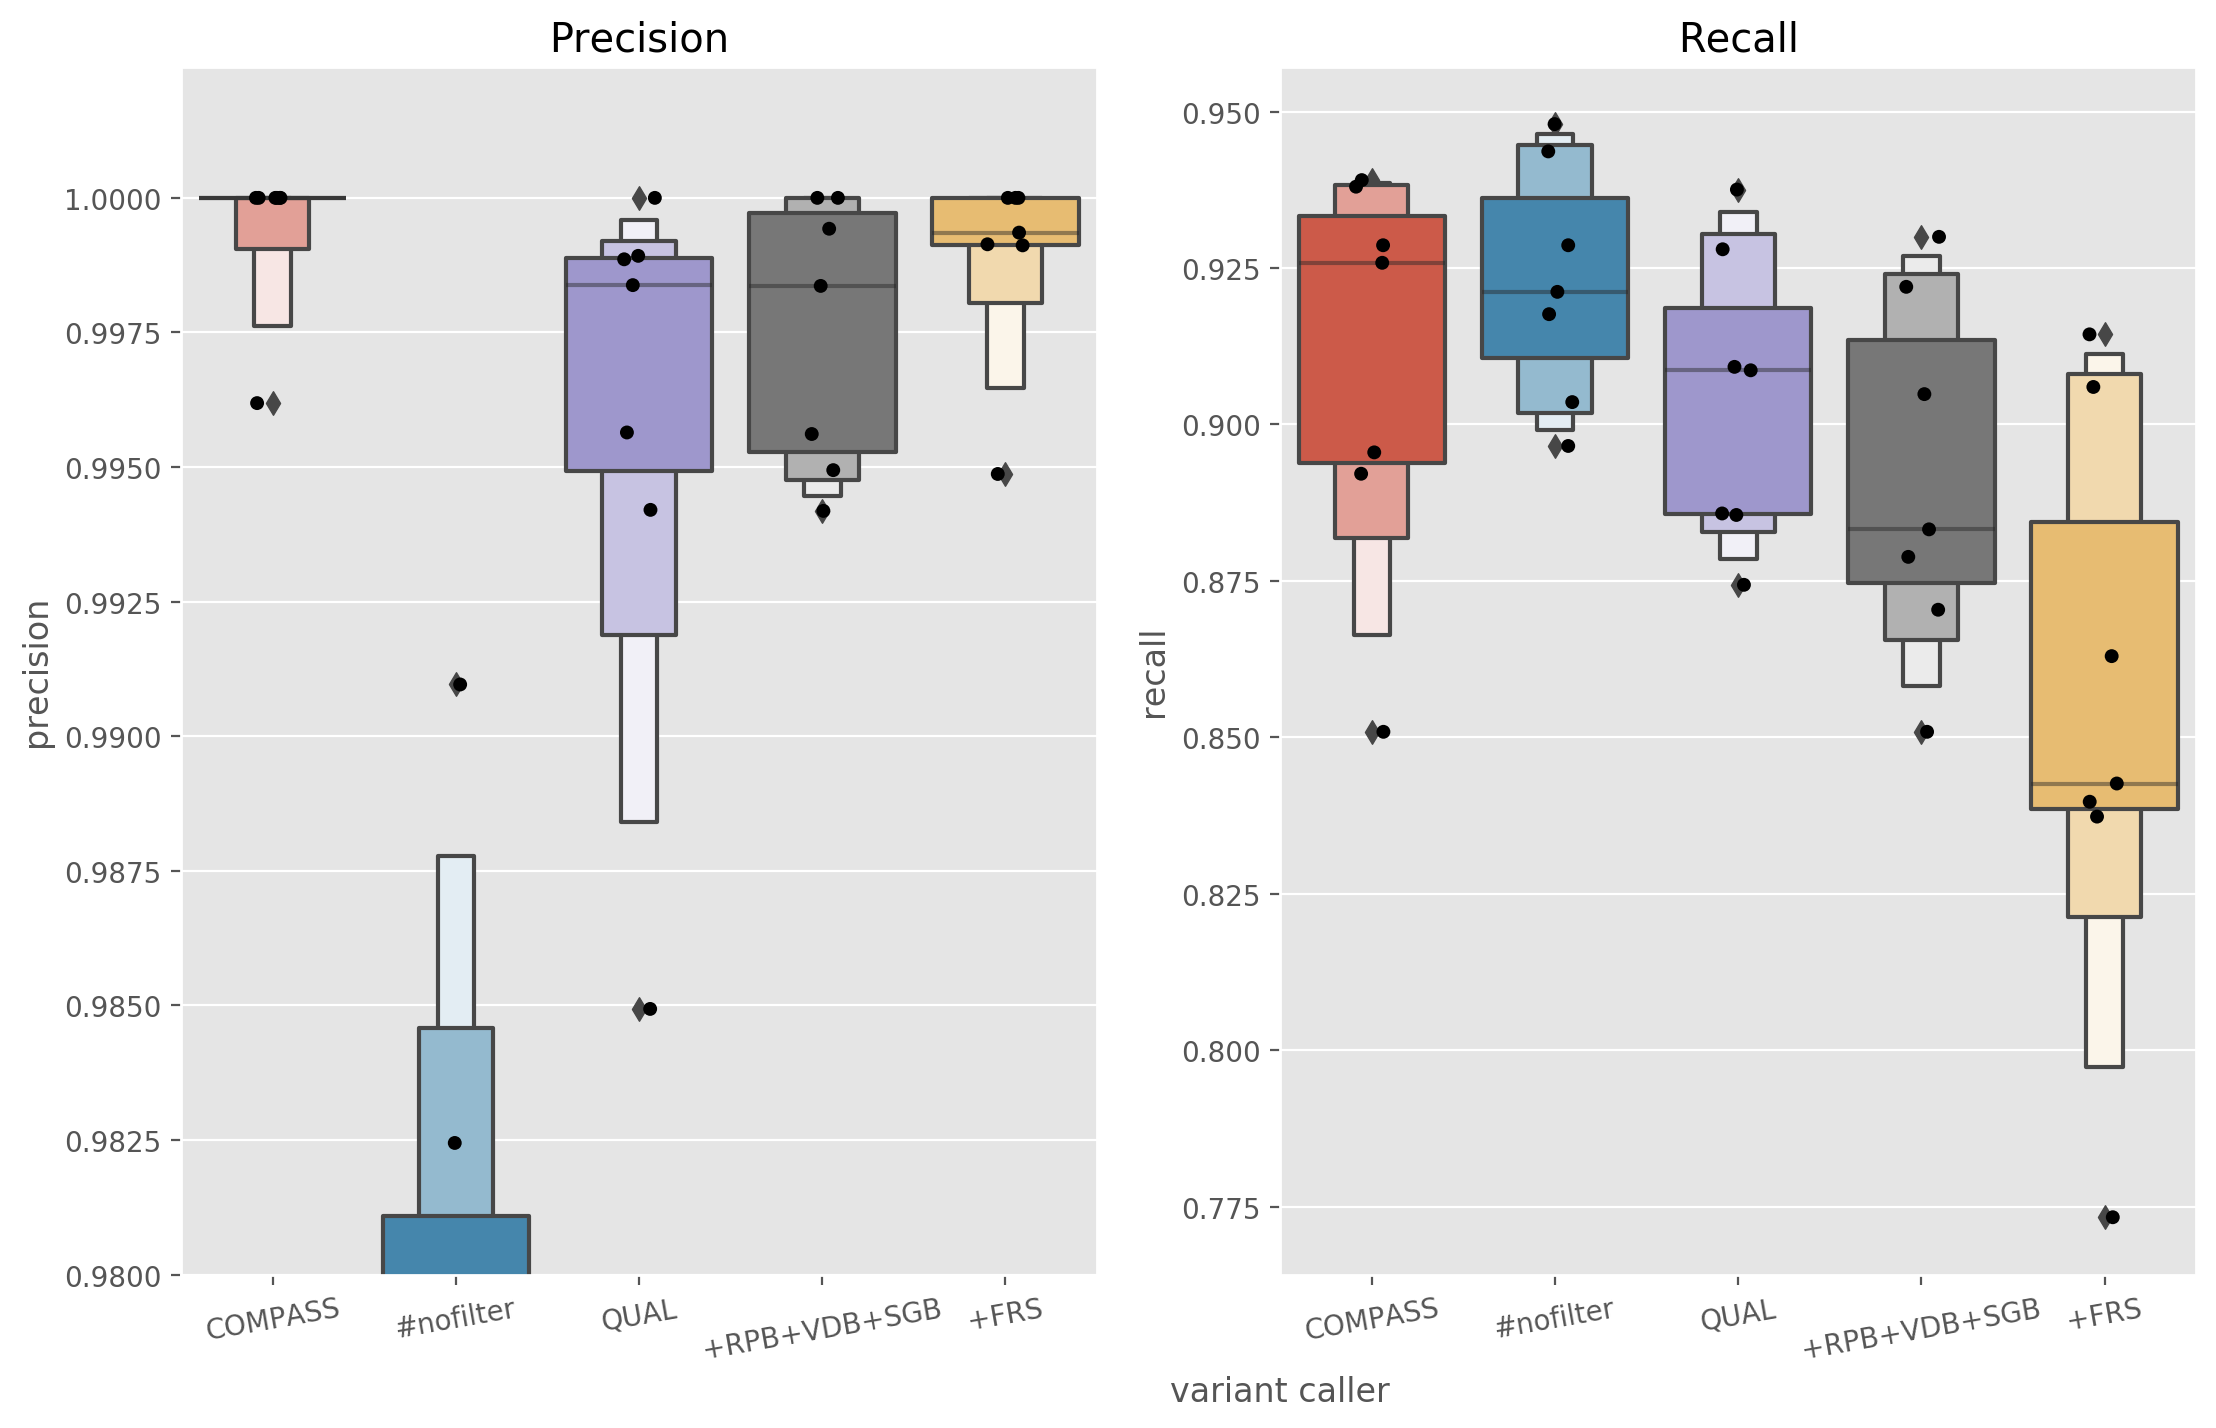
\includegraphics[width=0.90\columnwidth]{Chapter2/Figs/bcftools-precision-recall-filters.png}
\caption{{Precision (left) and recall (right) of SNPs for COMPASS (red) and a
selection of bcftools filters. \vrb{\#nofilter} (blue) is bcftools with no
filtering of variants. \vrb{QUAL} (purple) is bcftools SNPs with a quality score of
60 or more. \vrb{+RPB+VDB+SGB} (grey) indicates bcftools variants with the INFO
field values~\(\ge\)0.05,~\(\ge\)0.002,
and~\(\le\)-0.5, respectively, plus QUAL. \vrb{+FRS} (yellow) shows
bcftools SNPs with all previous filters, plus only SNPs where the
fraction of reads supporting the variant is at least 90\%. Note: the
precision plot y-axis was cut causing some \vrb{\#nofilter} points to be
hidden.
{\label{fig:bcftools-filters}}
}}
\end{center}
\end{figure}

\subsection{\ont{} variant calling: \pandora{}}
\label{sec:pandora-filters}

When assessing the best filters for increasing the precision of variant calls from \pandora{}, we are also interested in determining whether \prg{} density has a noticeable impact on performance. We use the sparse and dense \prg{}s from \autoref{sec:tbprg} and look at the precision and recall these produce for the same filters.

\subsubsection{Single-sample}
\label{sec:map-var-calls}

For each sample, we discover \denovo{} variants using the method outlined in \autoref{chap:denovo} using the \vrb{discover} command of \pandora{} (version 0.8.0). We use default parameters, except for limiting the number of novel variants from a candidate region to 10. Novel variants are added to the relevant local \prg{} using the same method as \todo{reference chapter 1 section that outlines how we feed de novo variants back into the PRG} and the resulting updated \prg{} is indexed with \pandora{}. The \vrb{map} routine of \pandora{} is then used to genotype a sample's reads and produce a VCF. To be able to compare the \pandora{} VCF to the truth assemblies we tell \pandora{} to output coordinates with respect to the H37Rv reference sequence for each locus. We then convert these locus positions to the absolute position within H37Rv. Running \pandora{} in this way leads to some alleles being quite long and having a lot of redundant information, so we use \vrb{bcftools norm} to trim unused alleles and reduce variants down to their most succinct representation. \\
The \pandora{} VCF fields we use for filtering are: the depth of coverage on the called allele, which we require at least 3 reads; we keep positions with a strand bias of at least 1\%, which is the lowest depth on the forward or reverse strand divided by the total depth; a genotype confidence score no less than 5; an FRS of at least 90\%  - calculated the same way as in \autoref{sec:bcftools-filters}.
The results of incrementally applying these filters, along with no filters and COMPASS, are shown in \autoref{fig:pandora-filters-snps}. Of the two \prg{}s used, \pandora{}'s best median precision (100\%) is with the sparse \prg{} and all filters applied. With all filters, the sparse \prg{} leads to a median recall of 71.99\%. When compared to the COMPASS median precision and recall values of 100\% and 92.58\%, respectively, \pandora{} produces \ont{} SNP calls with equivalent precision to Illumina, but with 20.59\% less recall (SNPs \emph{and} indels are assessed in \autoref{app:pandora-all-vars}). Part of the recall disparity between \pandora{} and COMPASS is explained by the masking of loci in the reference graph (see \autoref{sec:tbprg} and \autoref{app:mask}). Despite this large difference in recall, we chose to use all of the filters outlined above because, as mentioned earlier, precision is far more important than recall for the transmission cluster work.
In nearly every filtering combination, the sparse \prg{} lead to higher recall \emph{and} precision, albeit marginally. As a result, the remaining work featuring \pandora{} in this chapter will use the sparse \prg{} given the increased computational cost of using the dense \prg{}, without any benefit for precision and recall.

\begin{figure}
\begin{center}
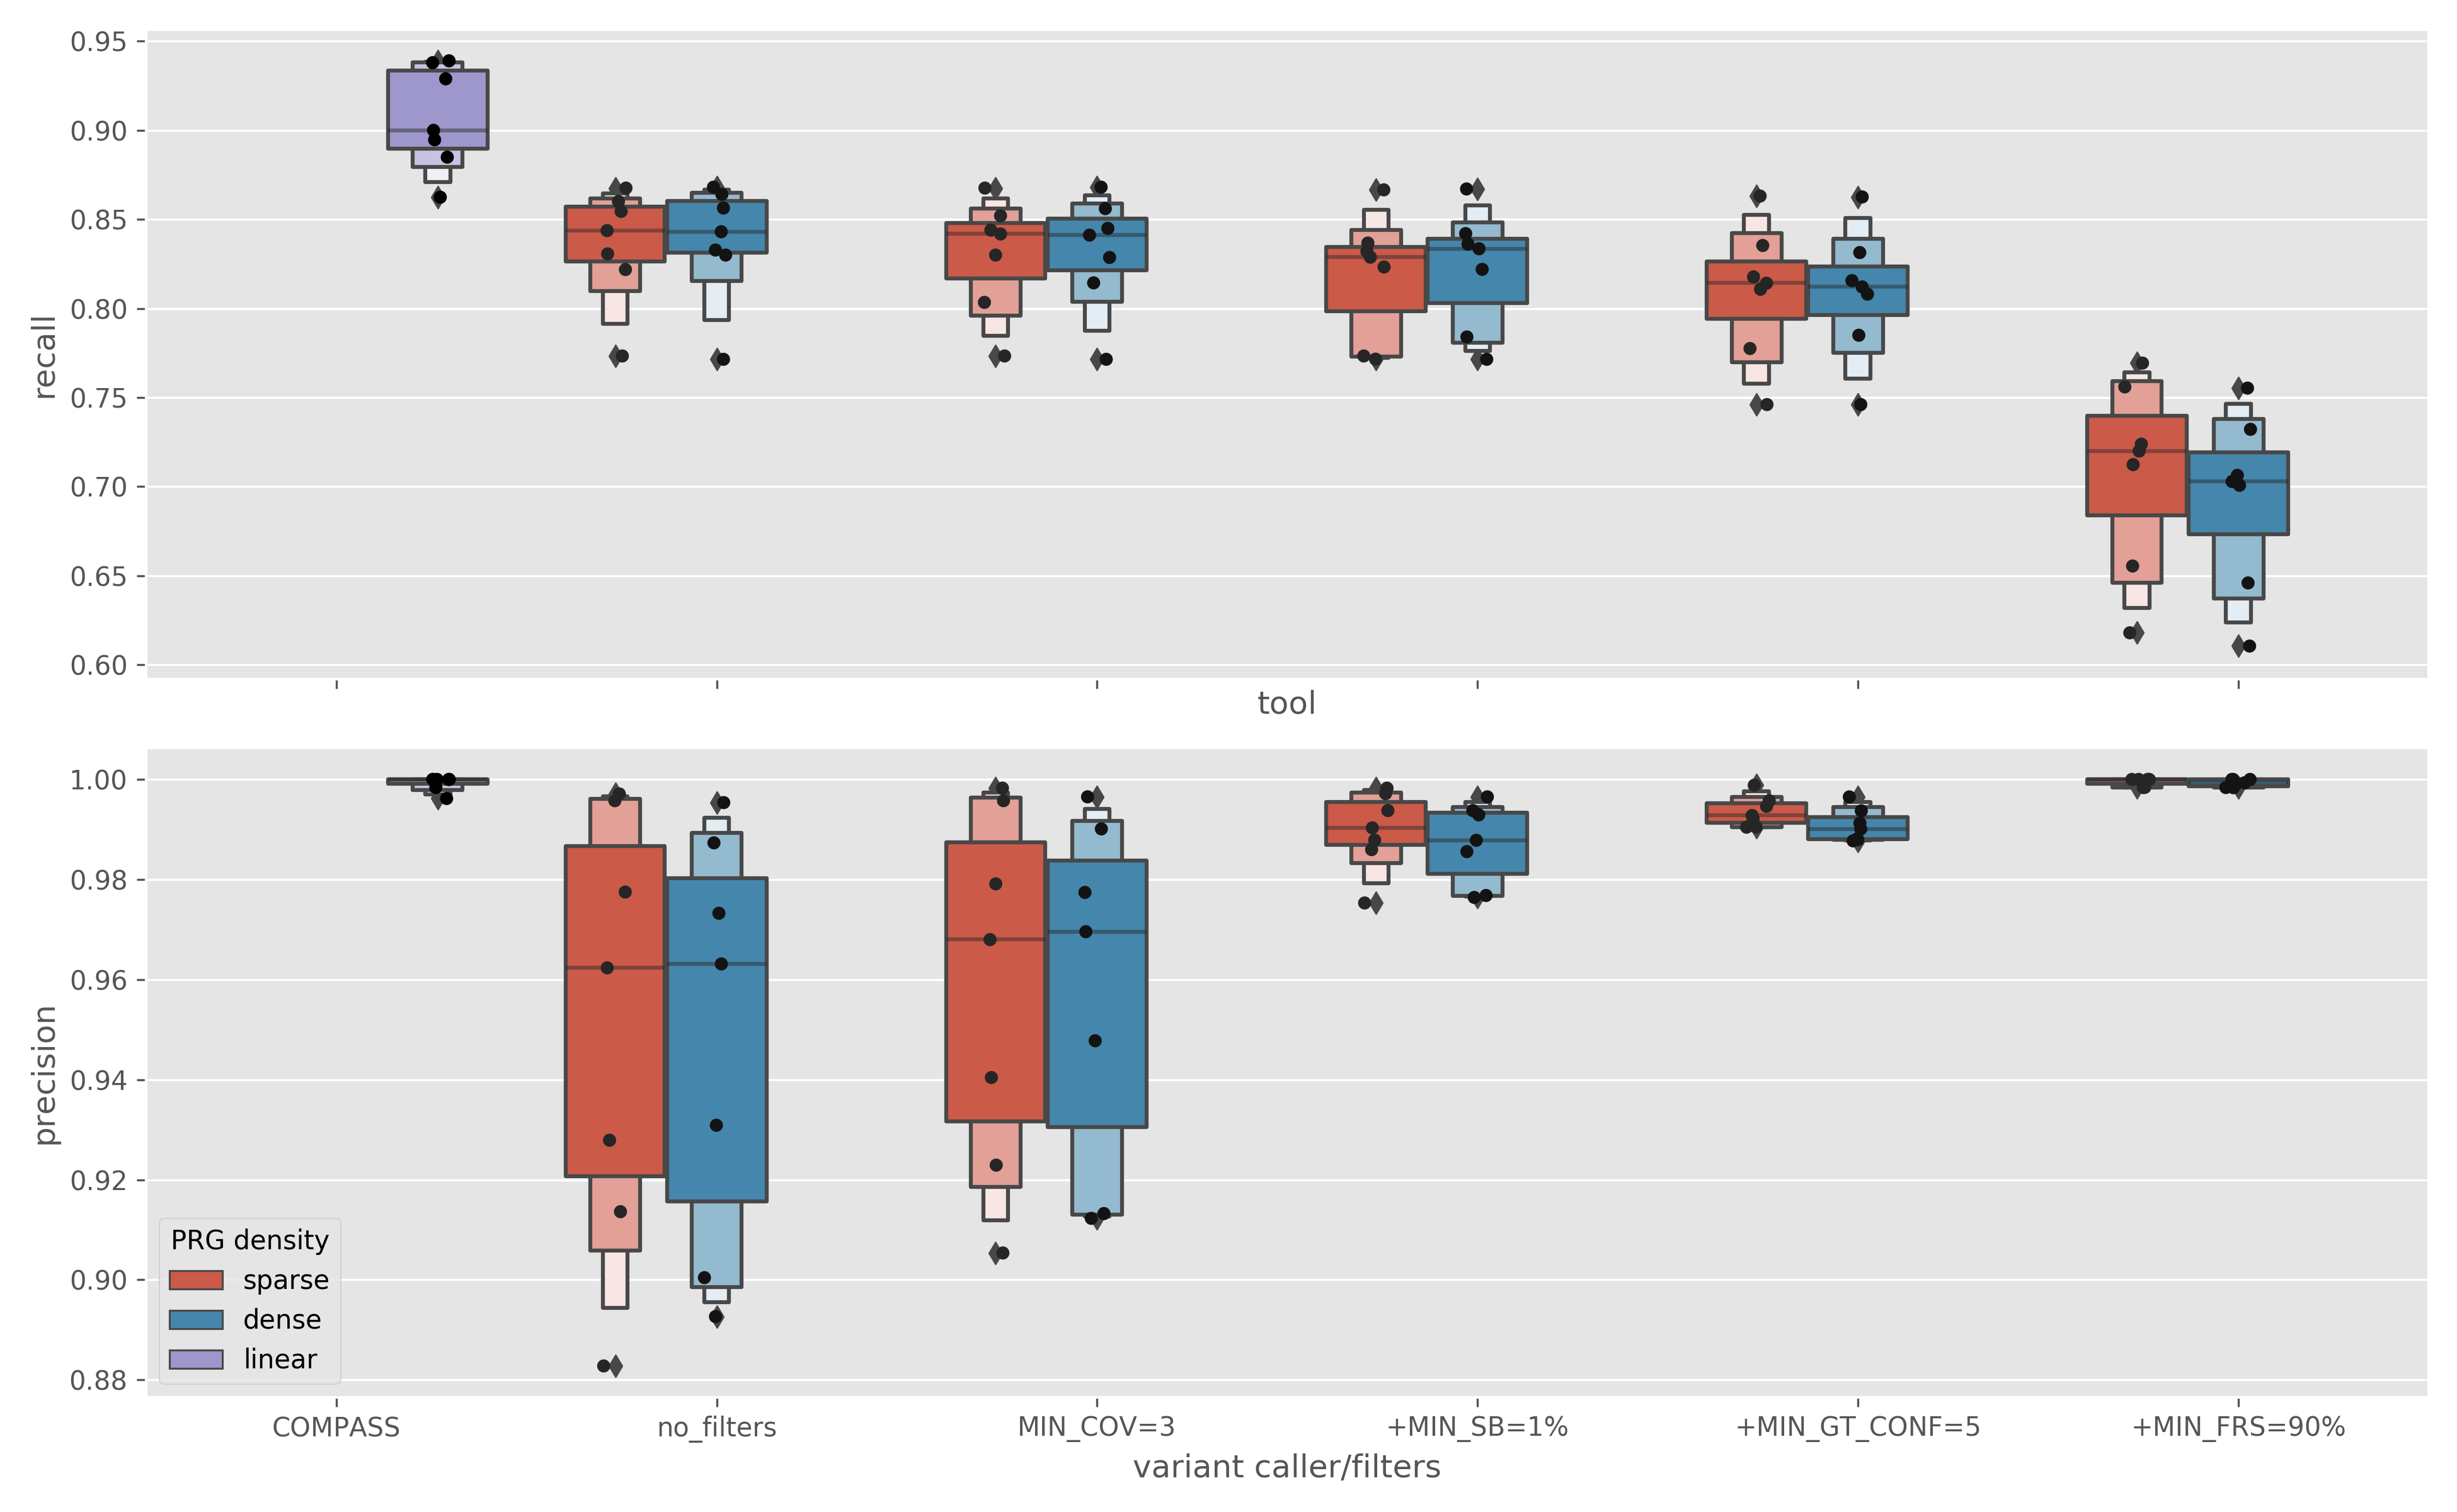
\includegraphics[width=0.90\columnwidth]{Chapter2/Figs/pandora-precision-recall-filters-snps.png}
\caption{{Precision (bottom) and recall (top) of SNPs for COMPASS (purple) and \pandora{} with sparse (red) and dense (blue) \prg{}s. The \pandora{} boxes start with no filters on the left, with each box moving to the right adding a filter to the previous box. The COMPASS box is a reference to the precision and recall of Illumina variant calls. Linear PRG density refers to the fact that COMPASS uses a single, linear reference genome as opposed to \pandora{}, which uses a genome graph. The black points refer to single data points for the seven samples used. MIN\_COV=minimum depth of coverage;MIN\_SB=minimum strand bias;MIN\_GT\_CONF=minimum genotype confidence score;MIN\_FRS=minimum fraction of read support.
{\label{fig:pandora-filters-snps}}%
}}
\end{center}
\end{figure}

\subsubsection{Multi-sample}

\pandora{}'s \vrb{map} routine infers a consensus sequence for a single sample and outputs variant calls with respect to that. However, \pandora{} also has a multi-sample counterpart - the \vrb{compare} command. The \vrb{compare} routine infers a single consensus sequence for \emph{all} samples and outputs a locus presense-absence matrix, along with a VCF of genotypes for all samples with respect to the consensus sequence \todo{link to ch1 or 2 section describing compare}. As it was designed for analysing collections of (potentially divergent) samples, we use the \vrb{compare} protocol to assess its ability to describe transmission clusters. 

The process for calling variants using \vrb{compare} is to first aggregate the novel variants discovered for each sample in \autoref{sec:map-var-calls}. Instead of creating an updated \prg{} for each sample, we take all novel variants for all samples and add them to the relevant locus' original MSA. We then update the MSA for each locus (from \autoref{sec:tbprg}), rebuild the \prg{}s for each locus, combine all local (locus) \prg{}s into a single pan-genome \prg{} and then index it with \pandora{}. In the end, we have a \prg{} that has novel variants from all samples contained within it, rather than the \prg{}s used by \vrb{map}, which only have the novel variants for a single sample.
Next, we run \vrb{pandora compare} using the updated sparse and dense \prg{}s and filter the resulting VCF as-per \autoref{sec:pandora-filters}.

As a result of its design, it is not possible to provide \vrb{compare} with a reference to base VCF coordinates on (as in \autoref{sec:map-var-calls}). Therefore, we cannot assess the precision and recall for the seven samples as above. We maintain the same filtering strategy as the single-sample approach though, as all of those fields are available in the VCF from \vrb{compare}.

\subsection{Computational performance}
\label{sec:var-call-comp-perf}

In addition to the quality of the variant calls, the computational cost of producing them is also important. The CPU time and maximum memory usage for performing the \ont{} variant calling is shown in \autoref{fig:var-comp-perf}. \pandora{}'s performance is broken down into the individual stages, while bcftools is represented by a single job (\vrb{pileup\_nanopore}). The median maximum memory for bcftools was 8.2GB, although, the maximum was as high as 58.5GB. This is compared to the highest \pandora{} step - updating the MSAs with novel variants - with a median maximum memory usage of 9.7GB and 13.3GB for the sparse and dense \prg{}s respectively. The highest memory usage for \pandora{} was 18.6GB during the updating of MSAs, nearly 40GB lower than the peak of bcftools. The median CPU time for bcftools was 35129 seconds, or 9.75 hours, with the longest run coming in at 138364 seconds (38.4 hours). To be able to compare this with \pandora{} as a whole, we can sum the median CPU time over each step, which gives 21704 and 53194 seconds, or 6.0 and 14.7 hours, for the sparse and dense \prg{}s respectively. As with the memory usage, the longest runtime component of the \pandora{} pipeline was updating the MSAs with \denovo{} variants.

The computational performance of \pandora{} \vrb{compare} is not directly comparable to bcftools and \pandora{} \vrb{map} as it runs on all samples at the same time. Additionally, the novel variant discovery phase of pandora map for all samples technically contributes to the overall runtime of compare. As the performance of this discovery step has already been reported, we outline the remainder of the steps involved in compare in \autoref{tab:compare-perf}. In total, the remainder of the sparse and dense \prg{} steps took 58.4 and 83.1 CPU hours respectively. The actual wall clock time for these steps was 5.5 and 7.3 hours. The maximum memory was again obtained during the updating of the MSAs and peaked at 38 and 37GB for the sparse and dense \prg{}s respectively.

\begin{figure}
     \centering
     \begin{subfigure}[b]{0.475\textwidth}
         \centering
         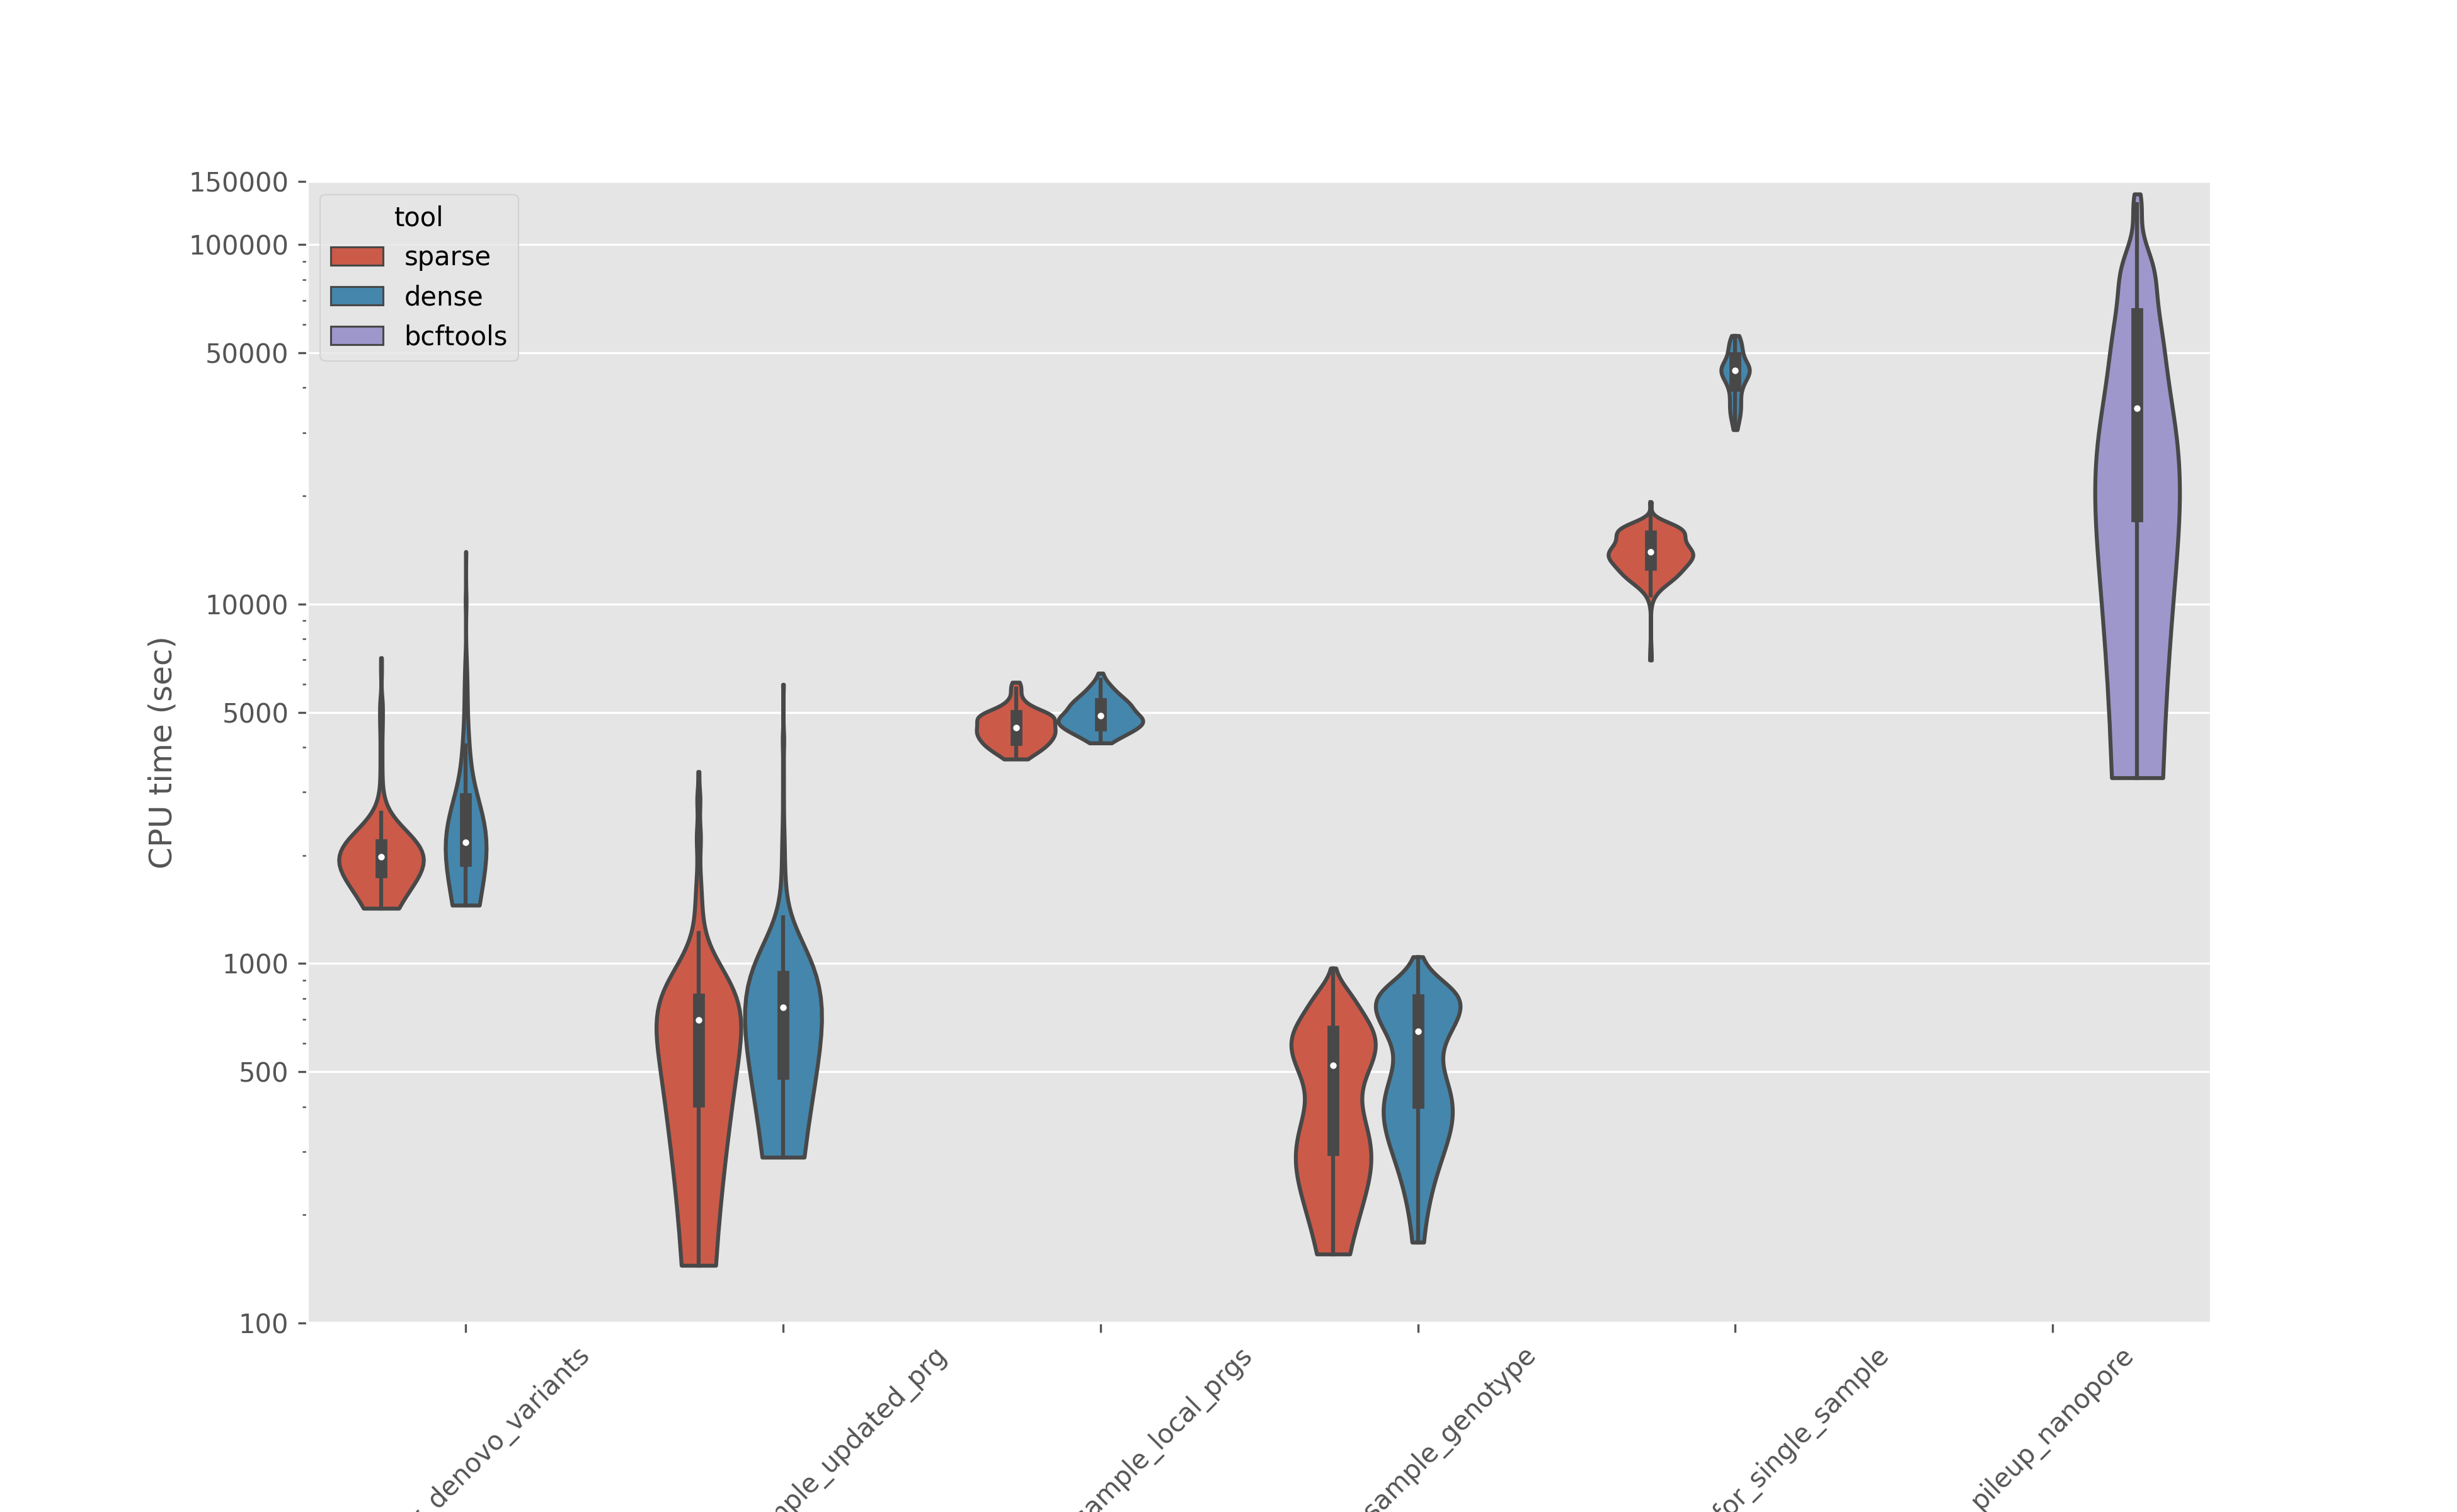
\includegraphics[width=\textwidth]{Chapter2/Figs/cpu_time.png}
         \caption{}
         \label{fig:cpu-time}
     \end{subfigure}
    %  \hfill
     \begin{subfigure}[b]{0.475\textwidth}
         \centering
         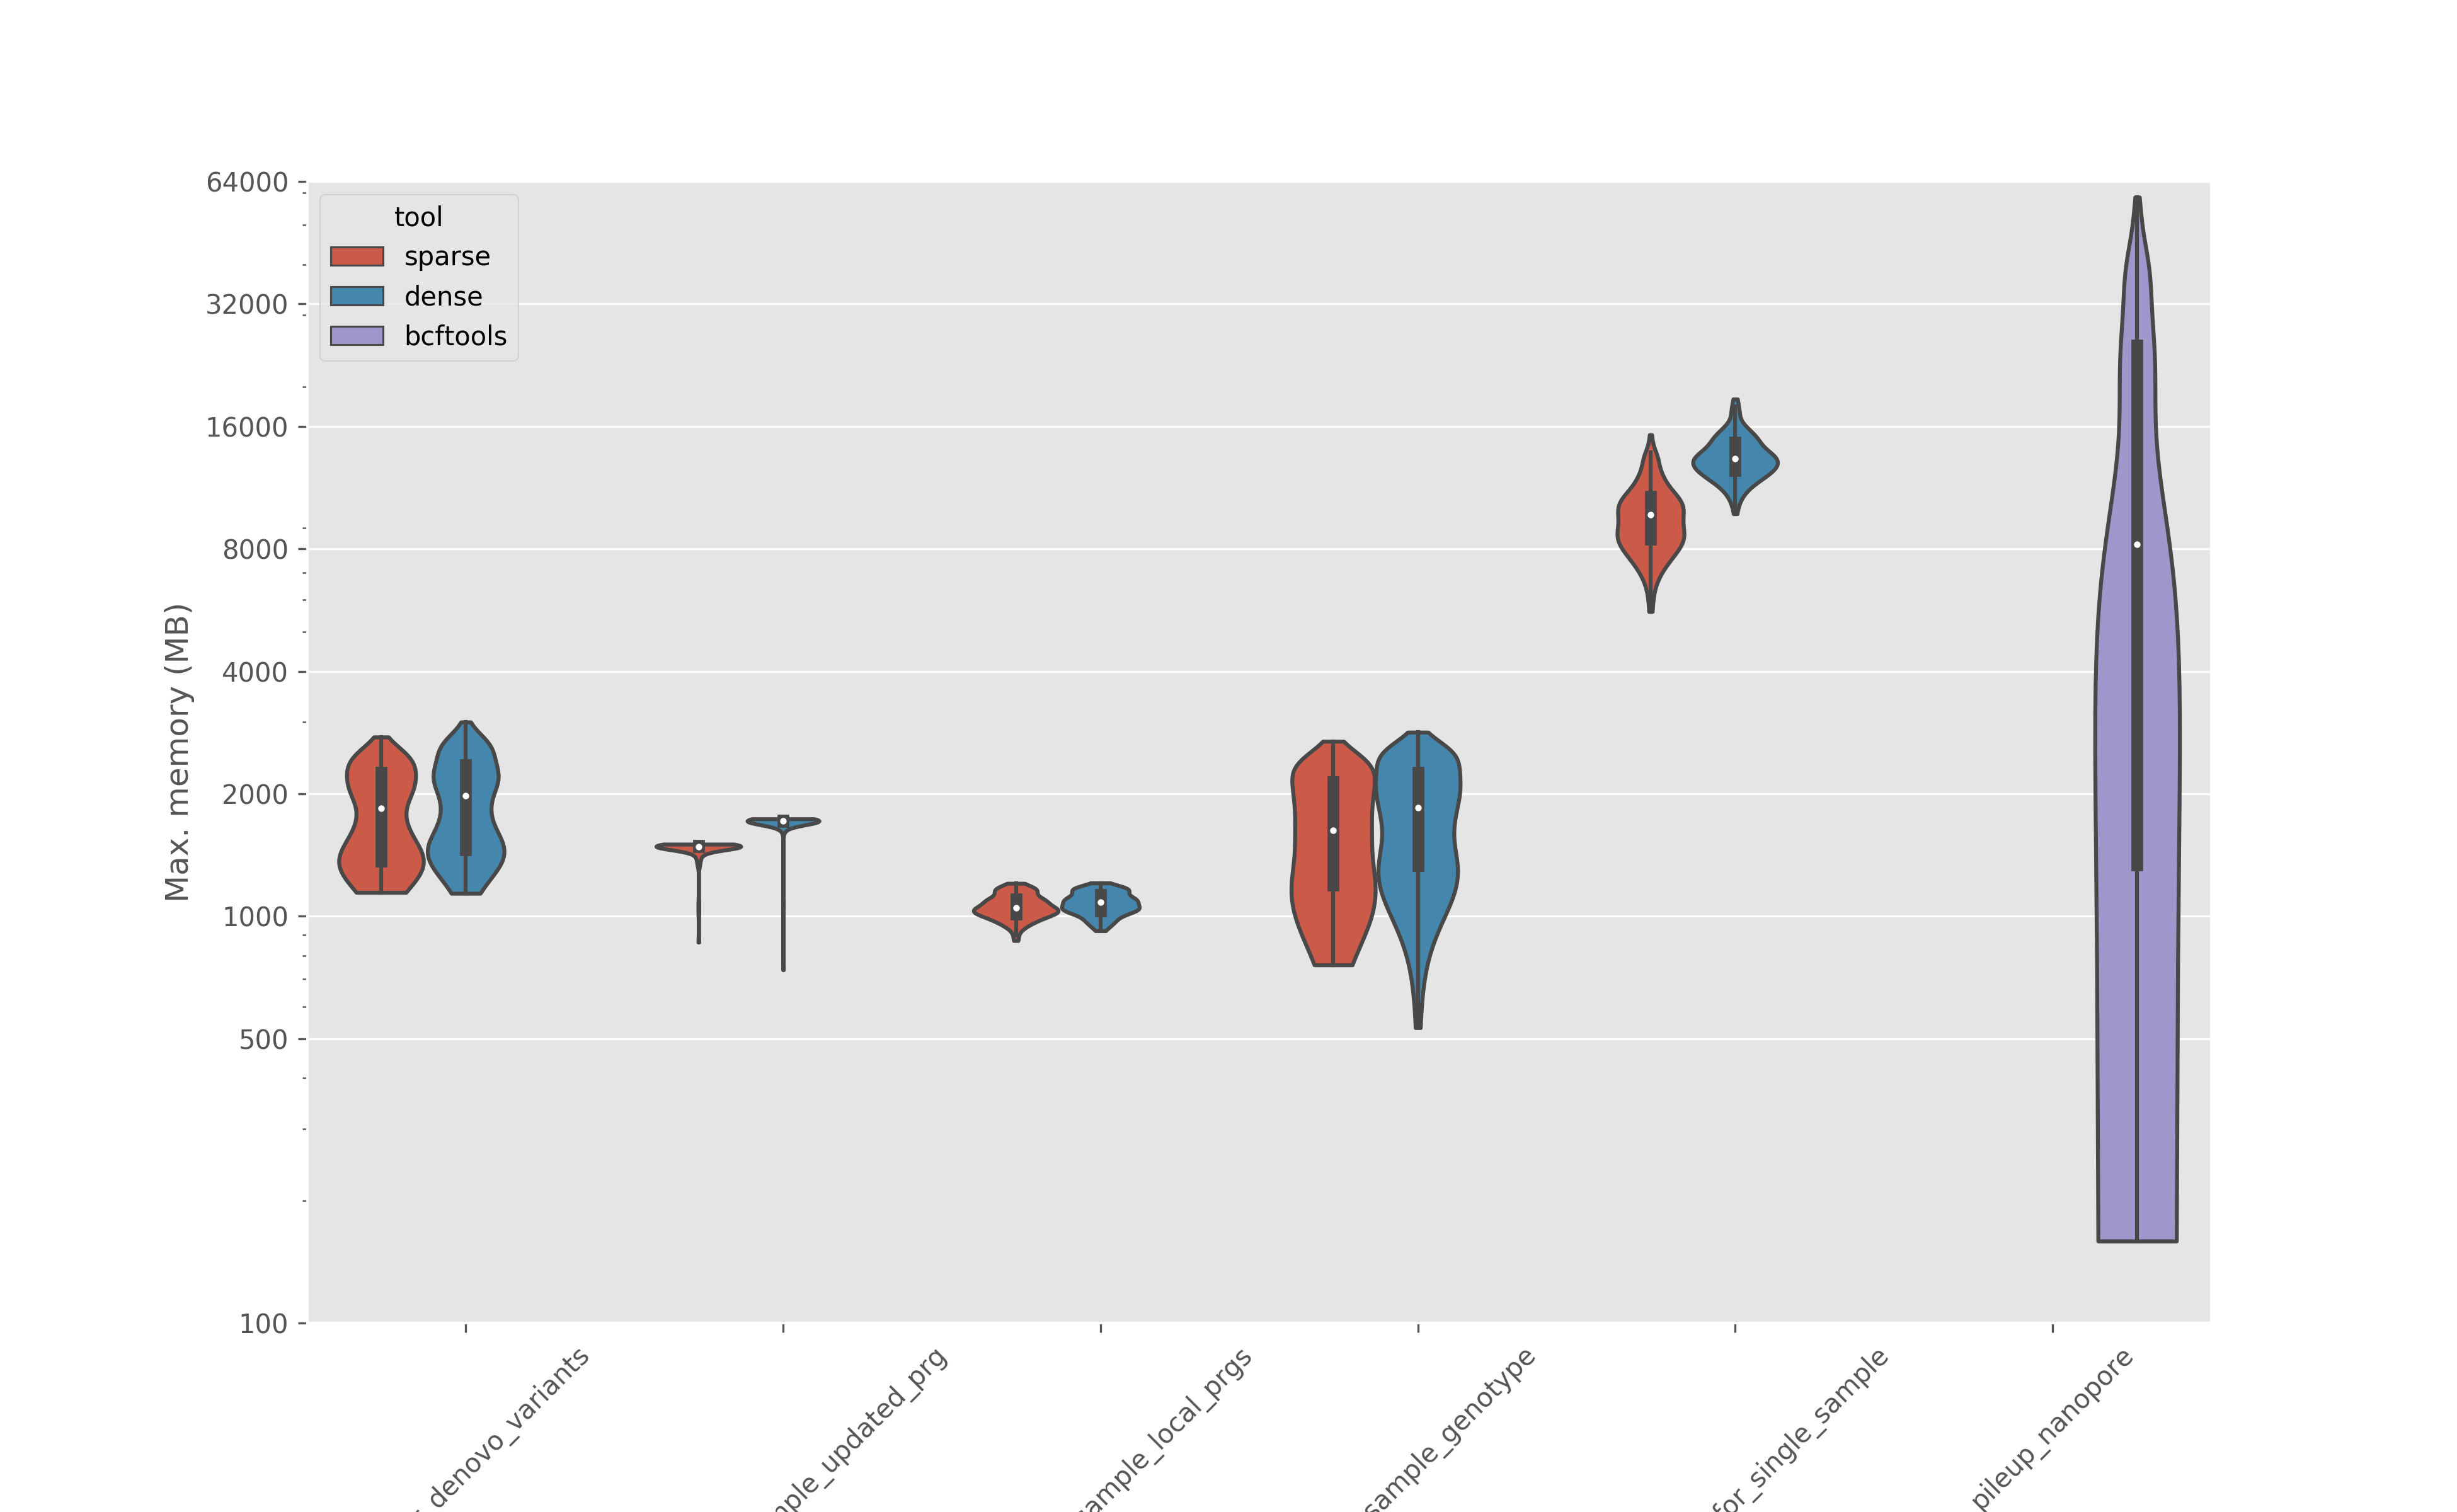
\includegraphics[width=\textwidth]{Chapter2/Figs/max_mem.png}
         \caption{}
         \label{fig:max-mem}
     \end{subfigure}
        \caption{The CPU time (in seconds; y-axis; \textbf{a}) and maximum memory usage (in megabytes; y-axis; \textbf{b}) for each \ont{} variant-calling job. Sparse (red) and dense (blue) refer to \pandora{} steps with the respective density \prg{}. \vrb{bcftools} (purple) only has one step (\vrb{pileup\_nanopore}). The violins represent the distribution of CPU time over all samples.}
        \label{fig:var-comp-perf}
\end{figure}

\begin{table}
\centering
\begin{tabularx}{\textwidth}{|l|X|X|X|X|X|X|}
\hline
         & \multicolumn{3}{l|}{Sparse}                          & \multicolumn{3}{l|}{Dense}                           \\ \hline
Step     & CPU time (sec) & Real time (H:m) & Max. RAM (GB) & CPU time (sec) & Real time (H:m) & Max. RAM (GB) \\ \hline
Update MSA      & 114677         & 1:01             & 38              & 130221         & 1:15             & 37              \\ \hline
Make PRG & 4700           & 0:05             & 1.2              & 5403           & 0:06             & 1.1              \\ \hline
Index    & 538            & 0:01             & 2.1              & 1224            & 0:02             & 2.4              \\ \hline
Compare    & 90486            & 4:25             & 5.4              & 162294            & 6:04             & 6.1              \\ \hline
\end{tabularx}
\caption{CPU and wall clock time, and memory (RAM) usage for the main steps of running \pandora{}'s multi-sample routine \vrb{compare}. Sparse and Dense refer to two different densities with respect to the number of variants used. All steps were run on a single compute node with 32 CPU cores. MSA=multiple sequence alignment;PRG=population reference graph.}
\label{tab:compare-perf}
\end{table}

\subsection{Summary}
\label{sec:var-summary}

In summary, \autoref{fig:prec-recall-filters} shows that our selection of filters for \ont{} variant callers provide precision on-par with Illumina. However, this precision comes at the cost of a loss in recall. The remainder of this chapter explores how the SNP calls from \ont{} can be used to calculate distances between samples, and define putative transmission clusters from these distances. We are especially interested in how similar the pairwise distances are between samples and sequencing modality and whether the same distance thresholds used for Illumina can also be used for \ont{}.

\begin{figure}
\begin{center}
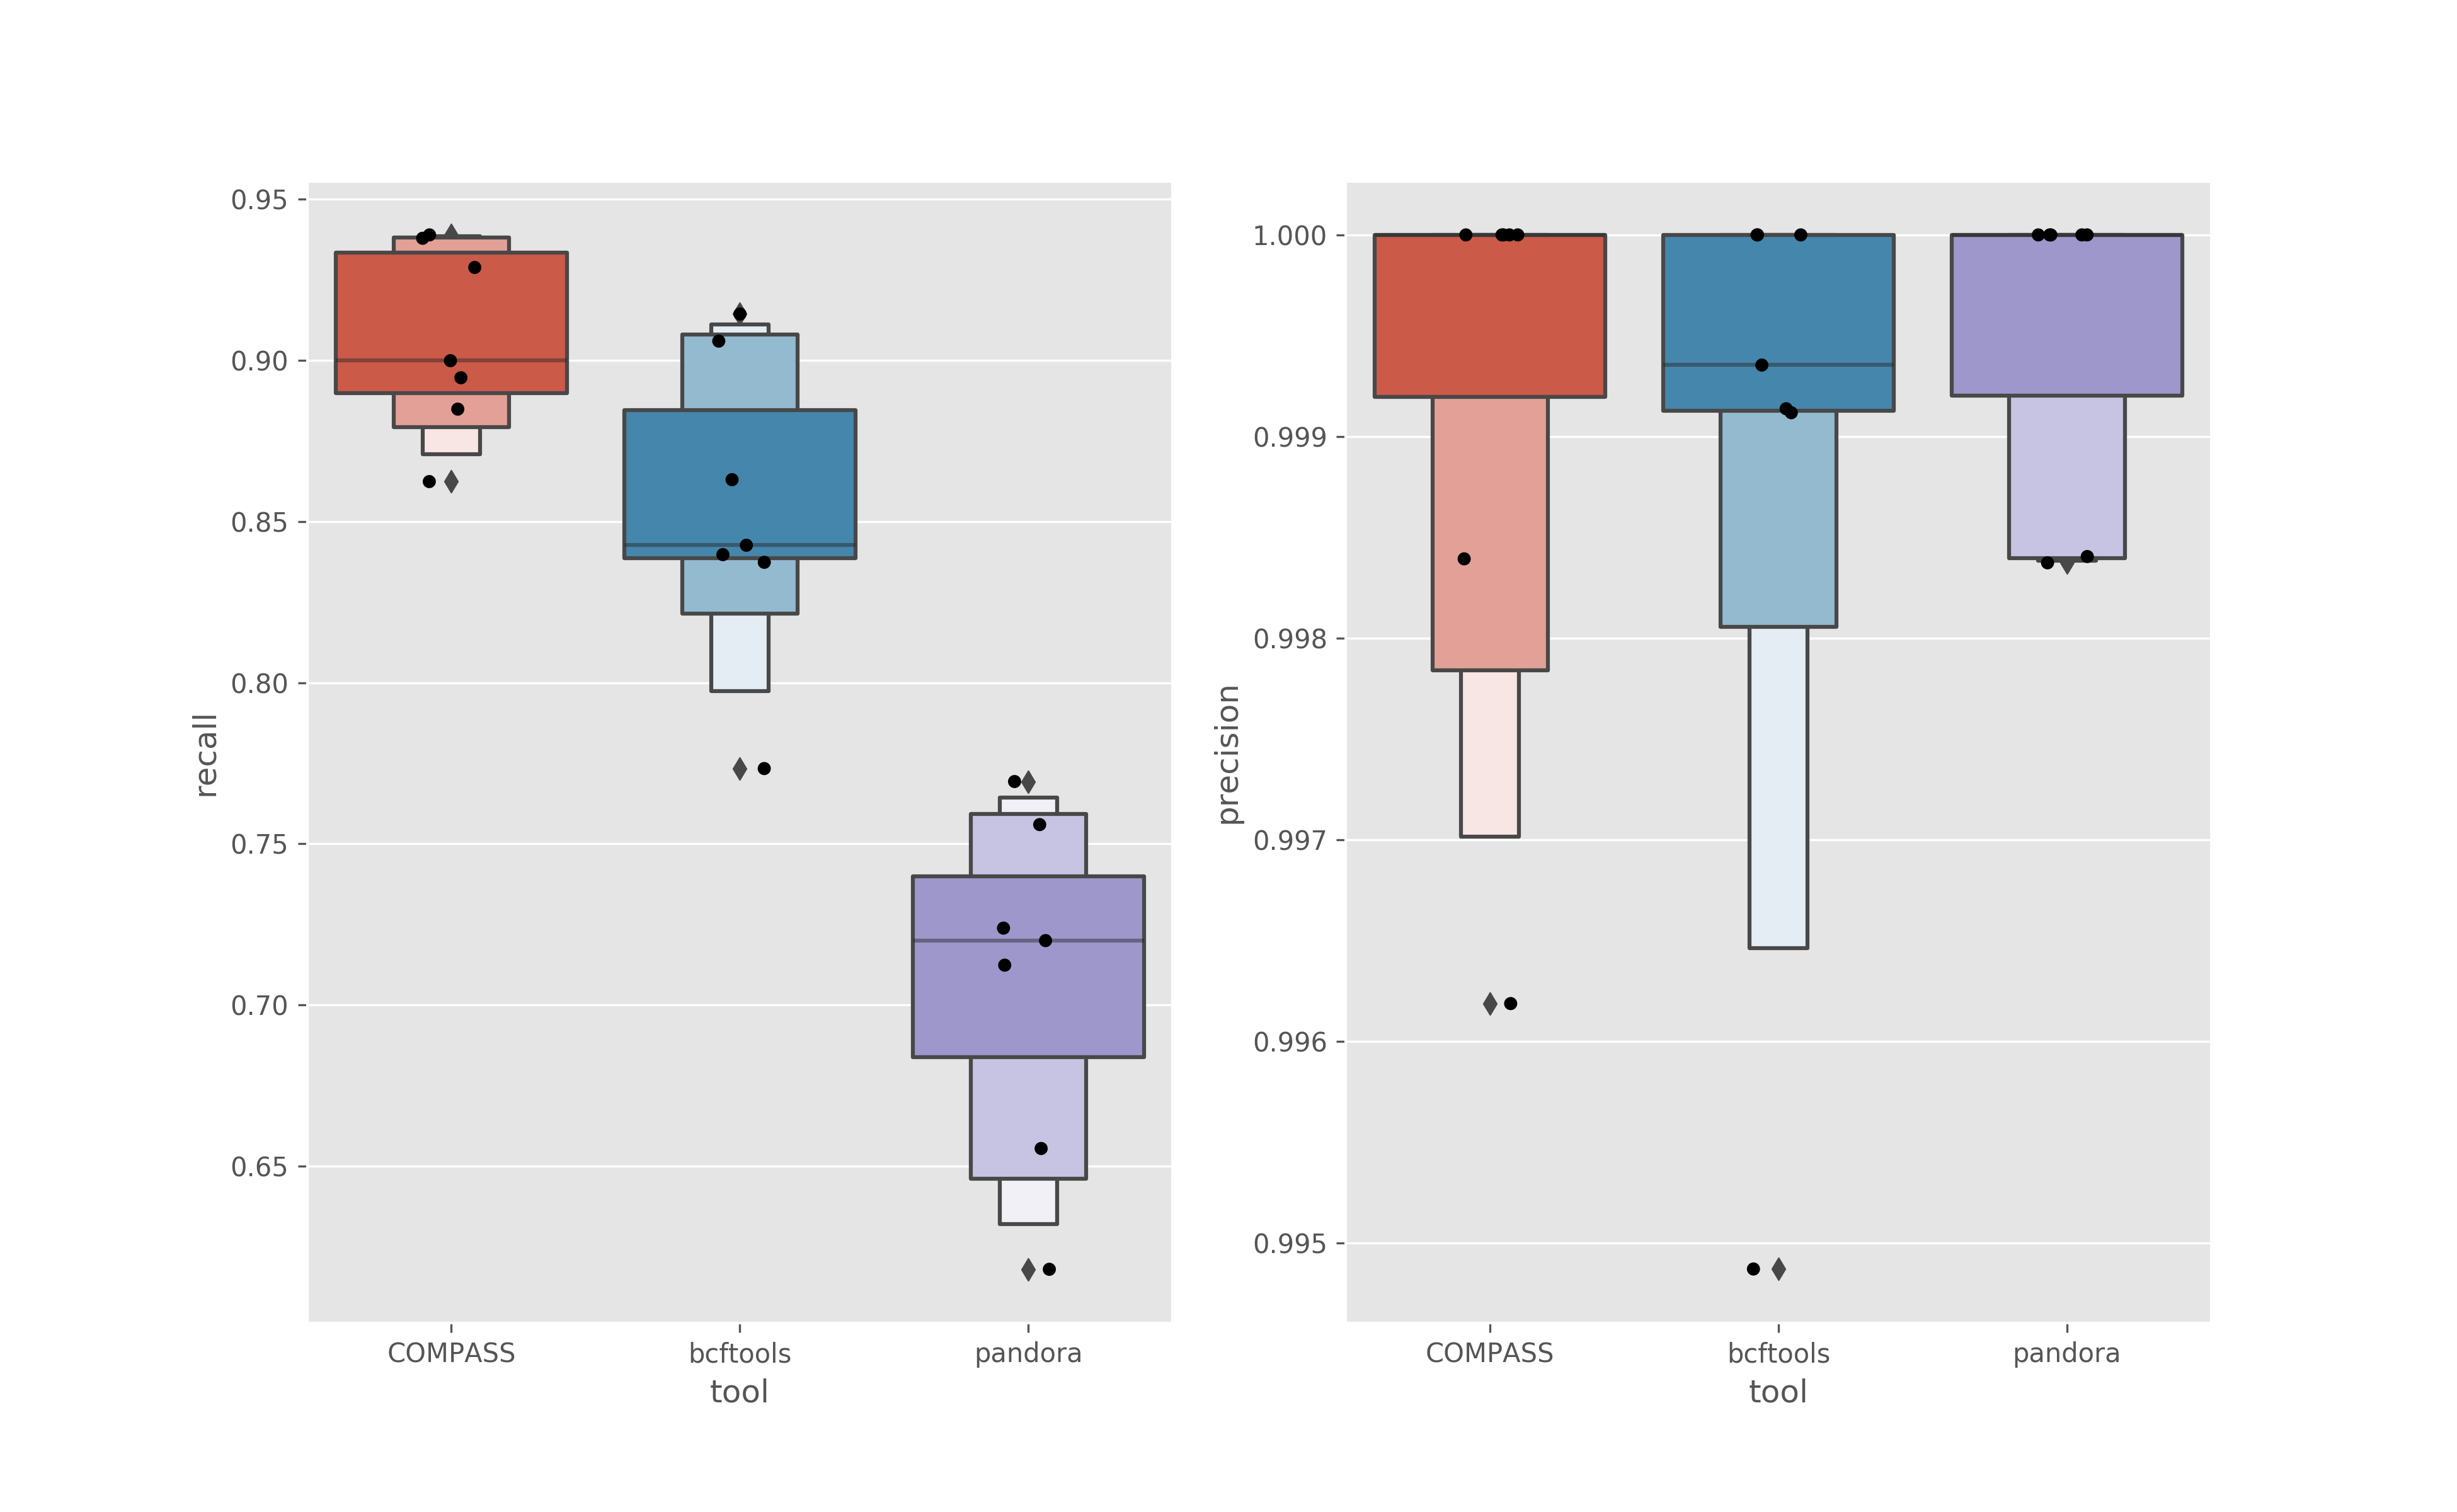
\includegraphics[width=0.9\columnwidth]{Chapter2/Figs/combined-precision-recall-filters-snps.png}
\caption{{Precision (left) and recall (right) of filtered SNPs for COMPASS (red), bcftools (blue), and \pandora{} (purple). Each black point represents one of seven evaluation samples. 
{\label{fig:prec-recall-filters}}%
}}
\end{center}
\end{figure}

%=========================================================================

\section{Pairwise SNP distance comparison for Illumina and \ont{} sequencing data}
\label{sec:snp-dist}

When attempting to infer transmission clusters, the one approach is
to define a SNP distance threshold and say that any genomes within this
distance of each other are clustered (possible transmissions). It follows that the SNPs used must
be trusted. Having shown that SNP precision on-par with Illumina can be
achieved with \ont{} data (see \autoref{sec:var-calls}), we investigate the pairwise SNP distance
between samples produced by both Illumina and \ont{} sequencing technologies. The intention
here is to determine whether the thresholds typically used for Illumina
data can also be used for \ont{}, or whether adjustments need to be
made.

To determine the distance between samples, we first generate sample consensus sequences. We do this for each variant-caller: COMPASS (Illumina), bcftools (\ont{}), and \pandora{}'s single-sample mode (\ont{}) (not \pandora{}'s multi-sample mode). A consensus sequence is obtained by applying the calls from a given VCF (from \autoref{sec:var-calls}) to the \mtb{} reference genome. We nullify (mark as \vrb{N}) any positions where i) the position failed filtering, ii) the reference genome position does not appear in the VCF file (except for \pandora{} single-sample), iii) the called genotype is null, or iv) the position is within the reference genome mask. All sample consensus sequences for a variant-caller are joined into a single FASTA file and a pairwise distance matrix is calculated using \vrb{snp-dists} (version 0.7.0) \cite{snp-dists}. In the case of \pandora{} \vrb{compare} (multi-sample mode), we cannot follow this approach for generating a consensus sequence and distance matrix, due to the inability to translate the coordinates from a graph to a linear reference. Instead of a consensus sequence, we generate a genotype array by extracting the called genotype for each sample at each site (VCF record). Where a site has failed a filter, we use a genotype value of -2. To calculate the distance between two samples, we compare their genotype arrays; if either sample's genotype is $<0$ (i.e. null or filtered) or the genotypes are the same, we record a distance of 0, otherwise 1. The sum of these comparisons for each genotype is the distance between the two samples.

The pairwise SNP distance relationship can be seen in \autoref{fig:dotplot}. For a given pair of samples, we plot their SNP distance, based on the COMPASS (Illumina) variant calls (x-axis), against the SNP distance for the same pair, based on the \ont{} variant calls (y-axis). All pairwise comparisons between a sample and itself were removed from the visualisation, and only a single value was used for each pair (i.e. we keep sample1 vs. sample2 and discard sample2 vs. sample1 as they are the same). RANSAC Robust Linear Regression \cite{fischler1981}, as implemented in the Python library \vrb{scikit-learn} \cite{scikitlearn}, was used for determining a linear equation and line-of-best fit for the relationship between pairwise Illumina and \ont{} SNP distance.

If the same thresholds used for Illumina can also be used for \ont{}, we would expect the distances to be the same and the bulk of the points in the plot to fall on the dashed, diagonal identity line in \autoref{fig:dotplot}. What we see instead is a linear relationship that falls \emph{under} this identity line - for all \ont{} variant callers. Given the filtered \ont{} SNP calls made by bcftools and \pandora{} have lower recall than Illumina (see \autoref{sec:var-summary}), this is expected, as they miss some SNPs found by Illumina.

One important observation though is highlighted by the zoomed inset in \autoref{fig:dotplot}. As SNP thresholds used for \mtb{} are generally well below 100 \cite{stimson2019}, it makes more sense to base SNP distance relationships on those samples that are "close". And indeed, when we zoom in on pairs of samples within 100 (Illumina) SNPs of each other, we see an association that is closer to the identity line. Fitting a linear model to this close subset of pairwise distances yields a relationship defined by the equation $y=0.806x+0.593$ for bcftools, $y=0.575x+13.544$ for \pandora{} single-sample, and $y=0.342x+0.765$ for \pandora{} multi-sample. Replacing $x$ with an Illumina SNP threshold gives the (predicted) equivalent \ont{} SNP threshold based on these relationships. For example, at an Illumina SNP distance of 12, the linear equation would predict a corresponding bcftools \ont{} SNP distance of 10.

\begin{figure}
\begin{center}
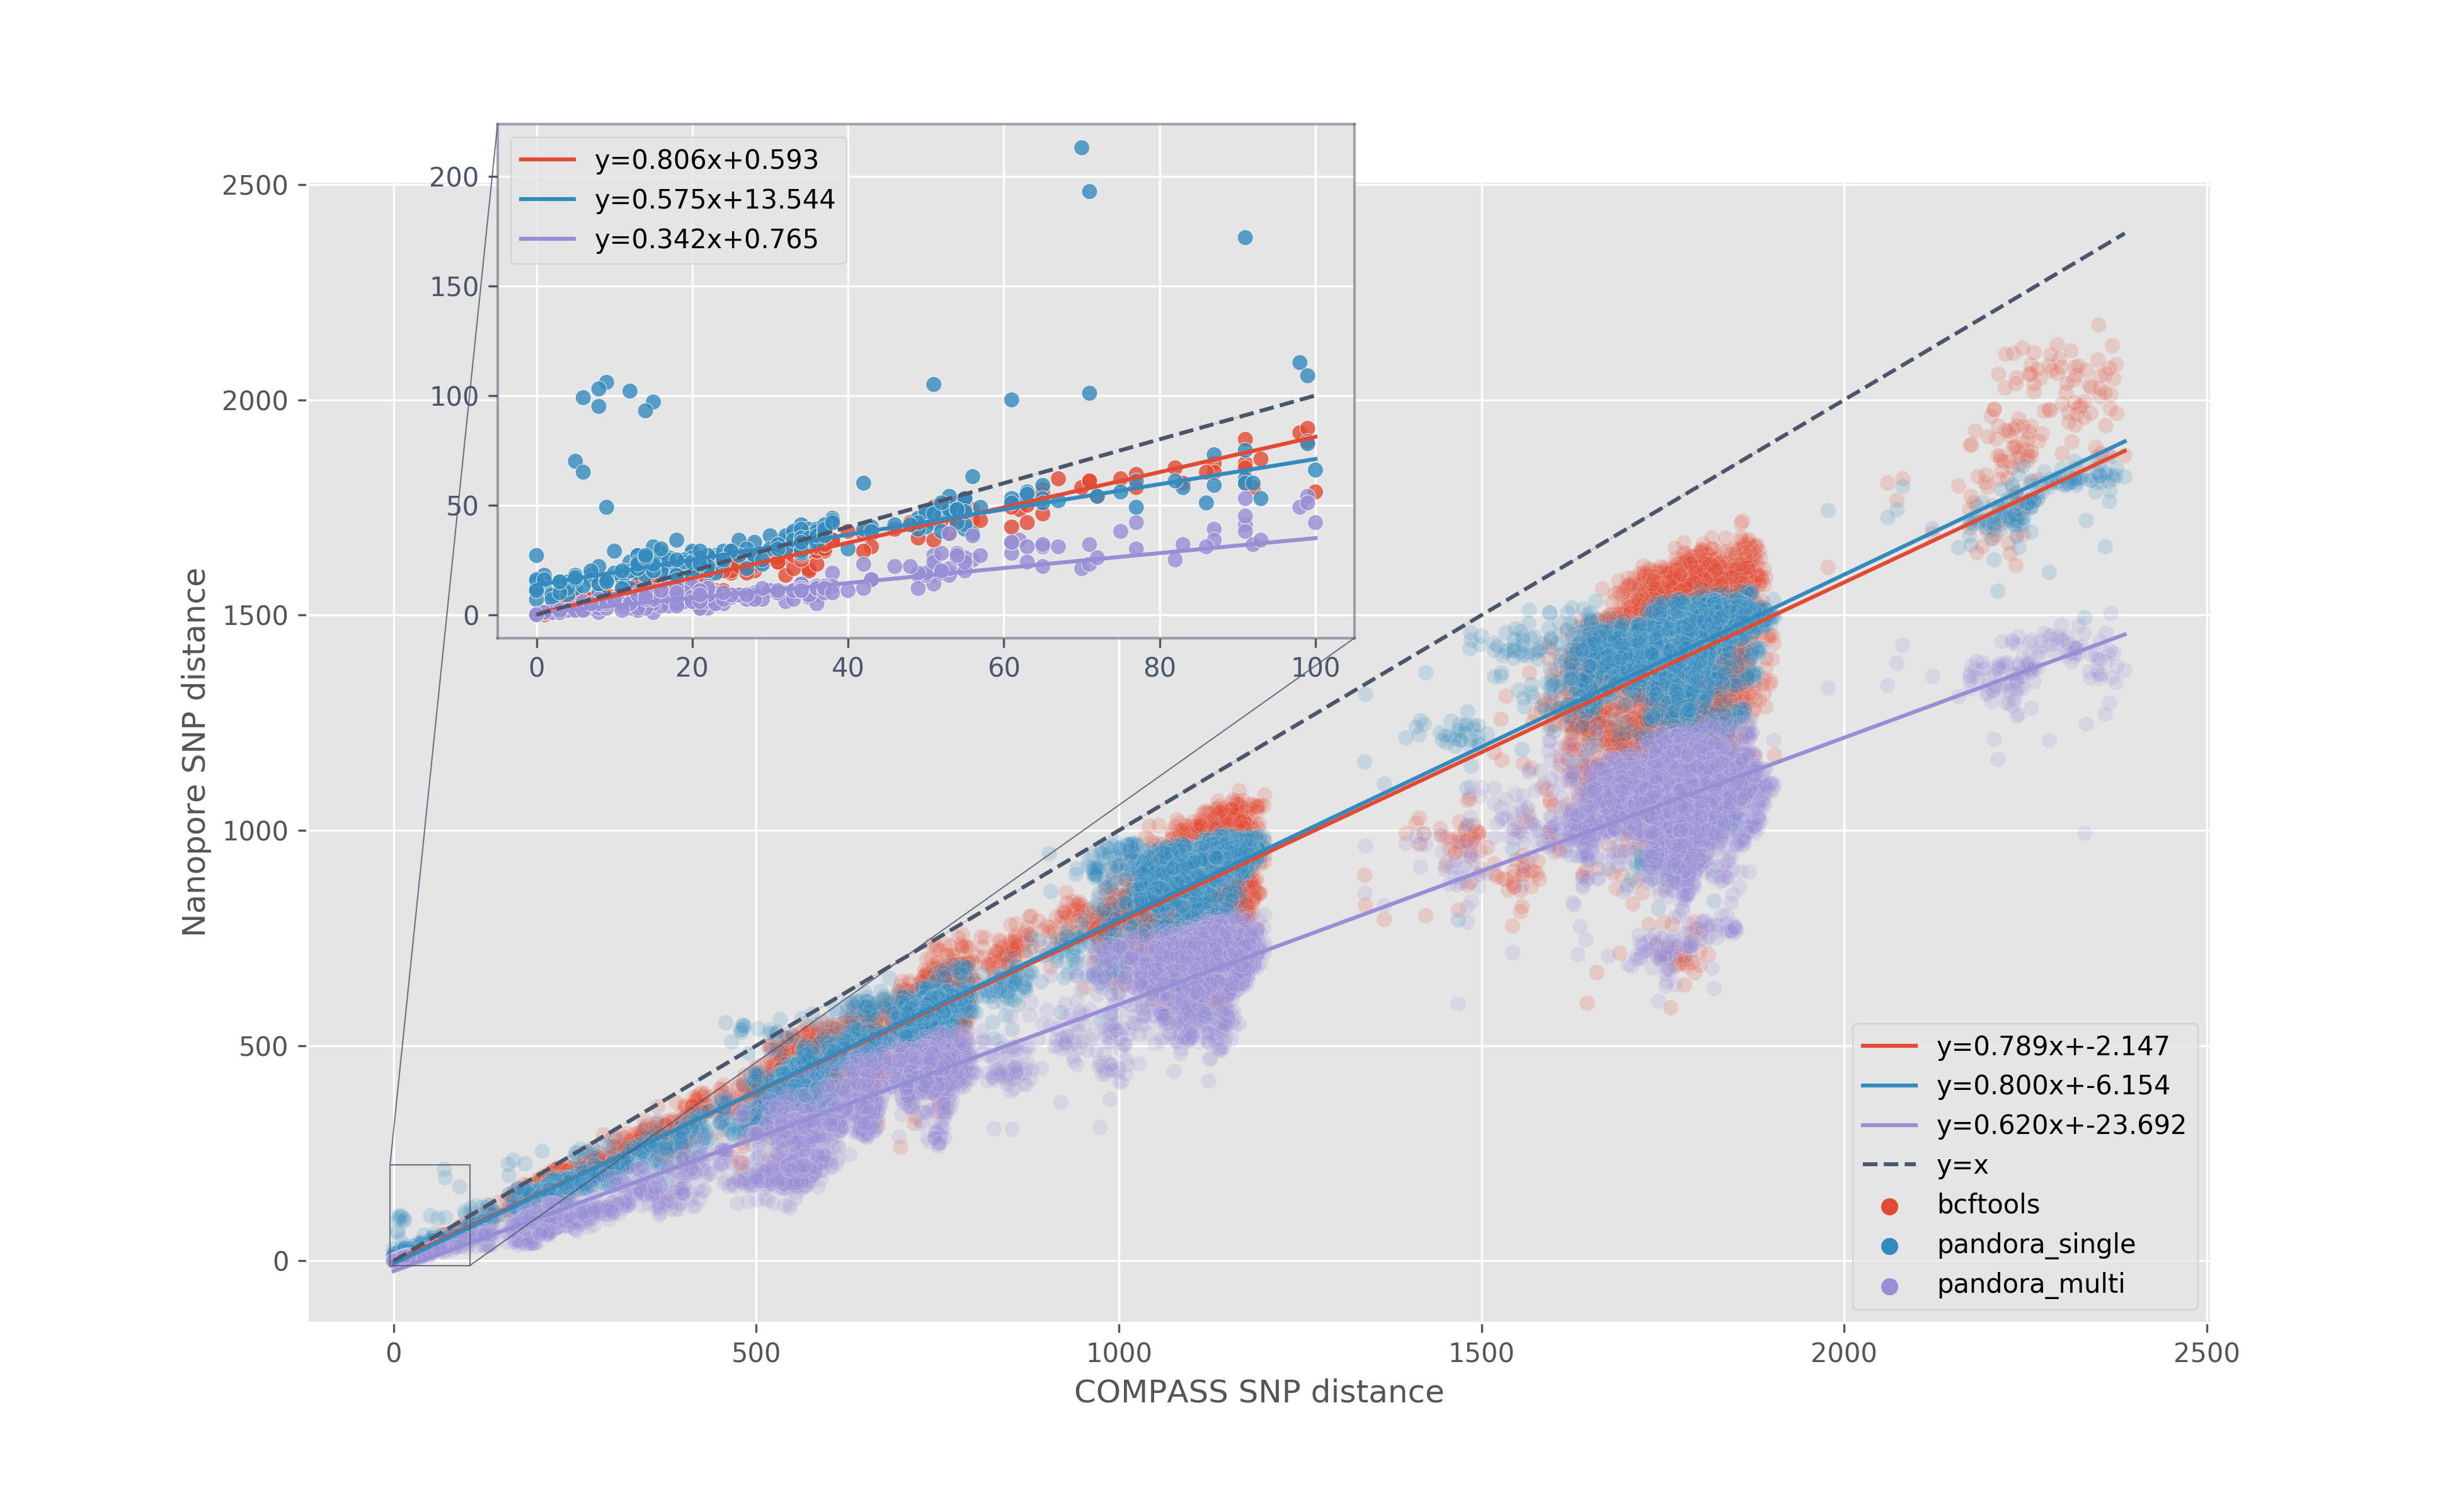
\includegraphics[width=0.90\columnwidth]{Chapter2/Figs/combined-dotplots.png}
\caption{{Pairwise SNP distance relationship between Illumina (COMPASS; x-axis) and \ont{} (bcftools (red), and \pandora{} single-sample (blue) and multi-sample (purple) mode; y-axis) data. Each point represents the SNP distance between two samples for the two sequencing modalities. The black, dashed line shows the identity line (i.e. $y=x$) and the coloured lines shows the line of best fit based on the robust linear model fit to the data. The zoomed inset shows all pairs where the COMPASS distance is $\le 100$.
{\label{fig:dotplot}}
}}
\end{center}
\end{figure}

%  see https://github.com/mbhall88/head_to_head_pipeline/issues/61 for a full investigation of the outliers discussed below
In the middle-left of the inset in \autoref{fig:dotplot} a small cluster of \pandora{} single-sample (blue) points can be seen. These have an approximate pairwise \ont{} distance of 100, but \texttildelow10 for Illumina. Upon further investigation, the cause of the large discrepancy in distance was due to \pandora{} single-sample failing to identify (and filter) a number of heterozygous calls. Two samples in particular occur as one member in all of the major outlying pairs. 94\% of the false positive differences leading to the large \ont{} distances occur at positions that are filtered due to evidence of heterozygosity in COMPASS. That is, in the Illumina consensus sequence these positions are ignored due to filtering and do not count as a difference. However, \pandora{} did not have sufficient read depth on both alleles to trigger the FRS filter (see \autoref{sec:pandora-filters}) - leading to a passing variant call that differs from the sample it is being compared with. \\

\noindent
The relationship between Illumina and \ont{} distances is indeed linear for all three variant-calling methodologies. While the relationship is not identical (i.e. a distance of 12 for Illumina does not necessarily mean a distance of 12 for \ont{}), we will attempt to use linear models fit to the relationship to infer what \ont{} SNP distance threshold is likely to align with a given Illumina threshold for defining putative transmission clusters.

%=========================================================================

\section{SNP threshold-based \ont{} transmission clustering}
\label{sec:clustering}

It is one thing to look at the relationship between Illumina and \ont{} pairwise SNP distance, but ultimately the most important question is: do \ont{} SNPs lead to transmission clusters consistent with those obtained with Illumina SNPs? To answer this question, we compare Illumina- and \ont{}-based clusters for four clinically-interesting (Illumina) SNP thresholds - 0, 2, 5, and 12. 

Selecting a SNP threshold to infer transmission clusters from has seen a variety of values recommended \cite{stimson2019}. As we seek to show concordance of \ont{} data with PHE's Illumina-based strategy, we opt to investigate Illumina threshold values 0, 2, 5, and 12. PHE define two cases as clustered if they have a SNP distance $\le 12$ as "\emph{12 SNPs represents the maximum SNP difference between 2 isolates for which epidemiological links have previously been identified \cite{walker2013} and is a conservative measure for reporting isolate relatedness}"\cite{phe-tb-england}. Five was likewise selected as it was found by \cite{walker2013} to indicate membership in a recent transmission chain. Threshold values 0 and 2 were chosen to provide insight into the level of granularity possible and is of clinical interest in certain settings (personal correspondence). For each of these four thresholds, we investigate what corresponding \ont{} SNP distance threshold yields the most similar clustering.

\subsection{Transmission cluster similarity}
\label{sec:cluster-similarity}

We use the distance matrices from \autoref{sec:snp-dist} to infer transmission clusters. In order to cluster samples, for a given SNP threshold $t$, we use only pairs of samples in the distance matrix with a distance $\le t$ to define a graph, $G=(V,E)$, where samples (nodes, $V$) are connected by weighted edges ($E$), with the weight of an edge indicating the distance between the two samples it connects. Clusters are defined as the set of connected components $\{C_1, C_2...C_N\}\in G$, where $N$ is the number of clusters. That is, a cluster (connected component), $C_i$, is a subgraph of $G$ where a path exists between any two samples in $C_i$, but no path exists to any samples in the rest of $G$. With this definition, all clusters have a minimum of two members. 

To assess how closely \ont{} SNP-based clustering approximates Illumina SNP-based clustering we adapt a similarity measure on sets, the Tversky Index \cite{tversky1977}. We define the Illumina clustering as $G$ and the \ont{} clustering as $H$. We are interested in being able to quantify the recall and precision of the \ont{} clustering, with respect to Illumina. In this sense recall would describe when samples that are clustered in $G$ are not clustered (or are in the wrong cluster) in $H$. Likewise, precision in this context tells us when extra samples are added to existing clusters by $H$, or when clusters in $G$ are joined in $H$. 

In order to be able to define precision and recall when comparing two clustering graphs $G$ and $H$ we define the Tversky Index

\begin{equation}
\label{eq:tversky-index}
   TI(n, G, H)=\frac{\left|C_{n,G}\cap C_{n,H}\right|}{\left|C_{n,G}\cap C_{n,H}\right|+\alpha |C_{n,G}-C_{n,H}|+\beta |C_{n,H}-C_{n,G}|}
\end{equation}

where $C_{n,G}$ is the cluster in $G$ that sample $n$ is a member of. When $\alpha = 1$ and $\beta=0$ in \autoref{eq:tversky-index}, we get a metric analogous to recall - as described above. Therefore, we define recall, $R$, for a single sample $n$ as

\begin{equation}
\label{eq:recall}
   R(n, G, H)=\frac{\left|C_{n,G}\cap C_{n,H}\right|}{\left|C_{n,G}\cap C_{n,H}\right|+|C_{n,G}-C_{n,H}|}=\frac{\left|C_{n,G}\cap C_{n,H}\right|}{|C_{n,G}|}
\end{equation}

When $\alpha = 0$ and $\beta = 1$ in \autoref{eq:tversky-index}, we get a metric analogous to precision. As such, we define precision $P$, for a single sample $n$ as

\begin{equation}
\label{eq:precision}
   P(n, G, H)=\frac{\left|C_{n,G}\cap C_{n,H}\right|}{\left|C_{n,G}\cap C_{n,H}\right|+|C_{n,H}-C_{n,G}|}=\frac{\left|C_{n,G}\cap C_{n,H}\right|}{|C_{n,H}|}
\end{equation}

With these definitions for a single sample, we can assess the recall and precision of the \ont{} clustering, $H$, with respect to the Illumina clustering, $G$, by averaging each metric over all samples in $G$. This gives us the Sample-Averaged Cluster Recall (SACR)

\begin{equation}
\label{eq:sacr}
   SACR=\frac{\sum_{n}^{V_G}R(n, G, H)}{|V_G|}
\end{equation}

where $V_G$ is the set of samples (nodes) in $G$ (Illumina graph). Likewise, we define the Sample-Averaged Cluster Precision (SACP) as 

\begin{equation}
\label{eq:sacp}
   SACP=\frac{\sum_{n}^{V_G}P(n, G, H)}{|V_G|}
\end{equation}

SACR states, on average, what proportion of the samples clustered together in $G$ are also clustered together in $H$ (\ont{}) - it is a measure of how many true positives \ont{} retains. Inversely, SACP states, on average, what proportion of the samples clustered together in $H$ are also clustered together in $G$ - it is a measure of how many extra samples \ont{} adds to clusters. However, SACR and SACP do not inherently account for when $H$ has clusters containing no samples in $G$. In order to quantify any extra clustering by $H$, we denote the Excess Clustering Rate (XCR) as the proportion of singletons (unconnected nodes) in $G$ that are (incorrectly) non-singletons in $H$. We define this as

\begin{equation}
\label{eq:xcr}
    XCR = \frac{|S_G-S_H|}{|S_G|}
\end{equation}

where $S_G$ and $S_H$ are the sets of singletons in the respective graphs. \\

\noindent
We assess the cluster similarities using the Python programming language with the \vrb{networkx} library \cite{networkx}. For a given threshold, we create the Illumina clustering (graph), $G$, and the \ont{} clustering, $H$ - as described above - and use these to calculate the SACR, SACP, and XCR using \autoref{eq:sacr}, \autoref{eq:sacp}, and \autoref{eq:xcr} respectively.

\subsubsection{Summary}

To summarise, for each sample in an Illumina-defined cluster, SACR is the proportion of samples in its Illumina cluster also in its \ont{} cluster - averaged over all samples. SACP is the proportion of samples in its \ont{} cluster also in its Illumina cluster - averaged over all samples. SACR indicates whether samples have been missed from \ont{} clustering (false negatives) and SACP reveals if additional samples are being added to \ont{} clusters (false positives). One shortcoming of SACR and SACP is they do not account for when the \ont{} clustering contains clusters where no member of the cluster is part of an Illumina cluster. To that end, XCR is the proportion of Illumina non-clustered (singleton) samples that are added to a cluster by \ont{}. An XCR value of 0.1 would indicate that 10\% of non-clustered samples were actually part of a cluster in the \ont{} clustering. An illustrated, worked example of these metrics can be found in \autoref{app:cluster-example}.

Of the metrics outlined above, our major focus is SACR, as missing samples from clusters is of particular concern for public health authorities.

\subsection{Evaluating \ont{} transmission clusters}
\label{sec:eval-clusters}

\subsubsection{bcftools}
\label{sec:bcftools-clustering}

For the four Illumina SNP distance thresholds of interest - 0, 2, 5, and 12 - the corresponding bcftools thresholds we use are 0, 2, 5, and 11. We chose to forego the model-based predicted thresholds and instead use the hand-picked ones based on a threshold parameter-sweep outlined in \autoref{app:dist-sweep}.

\autoref{fig:bcftools-clusters} is a visualisation of these clustering results for bcftools. The graphs depict the true (Illumina/COMPASS) clusters for each SNP threshold. The inner and outer colours of each node represent the SACR and SACP values, respectively, for the cluster it is a member of. The actual clustering produced by bcftools - without any annotations - can be see in \autoref{fig:bcftools-original-clusters}.

The bcftools clustering results are summarised in \autoref{tab:bcftools-cluster-summary} for all four SNP thresholds analysed. Of note, bcftools achieves a SACR of 1.0 at all thresholds - meaning \ont{} does not miss any samples from their correct clustering. At the SNP threshold of 2, bcftools clustering only differed from Illumina by the addition of one sample to a cluster of three.  SNP threshold 5 had the highest XCR (0.057), due to two new clusters of size 2 and 3, and the addition of 2 singleton samples to a cluster of 5.  The lowest SACP was at threshold 12. This is explained by two cases of a cluster of 2 being added to a larger cluster and 3 singletons being added to existing clusters. 

\begin{figure}
\begin{center}
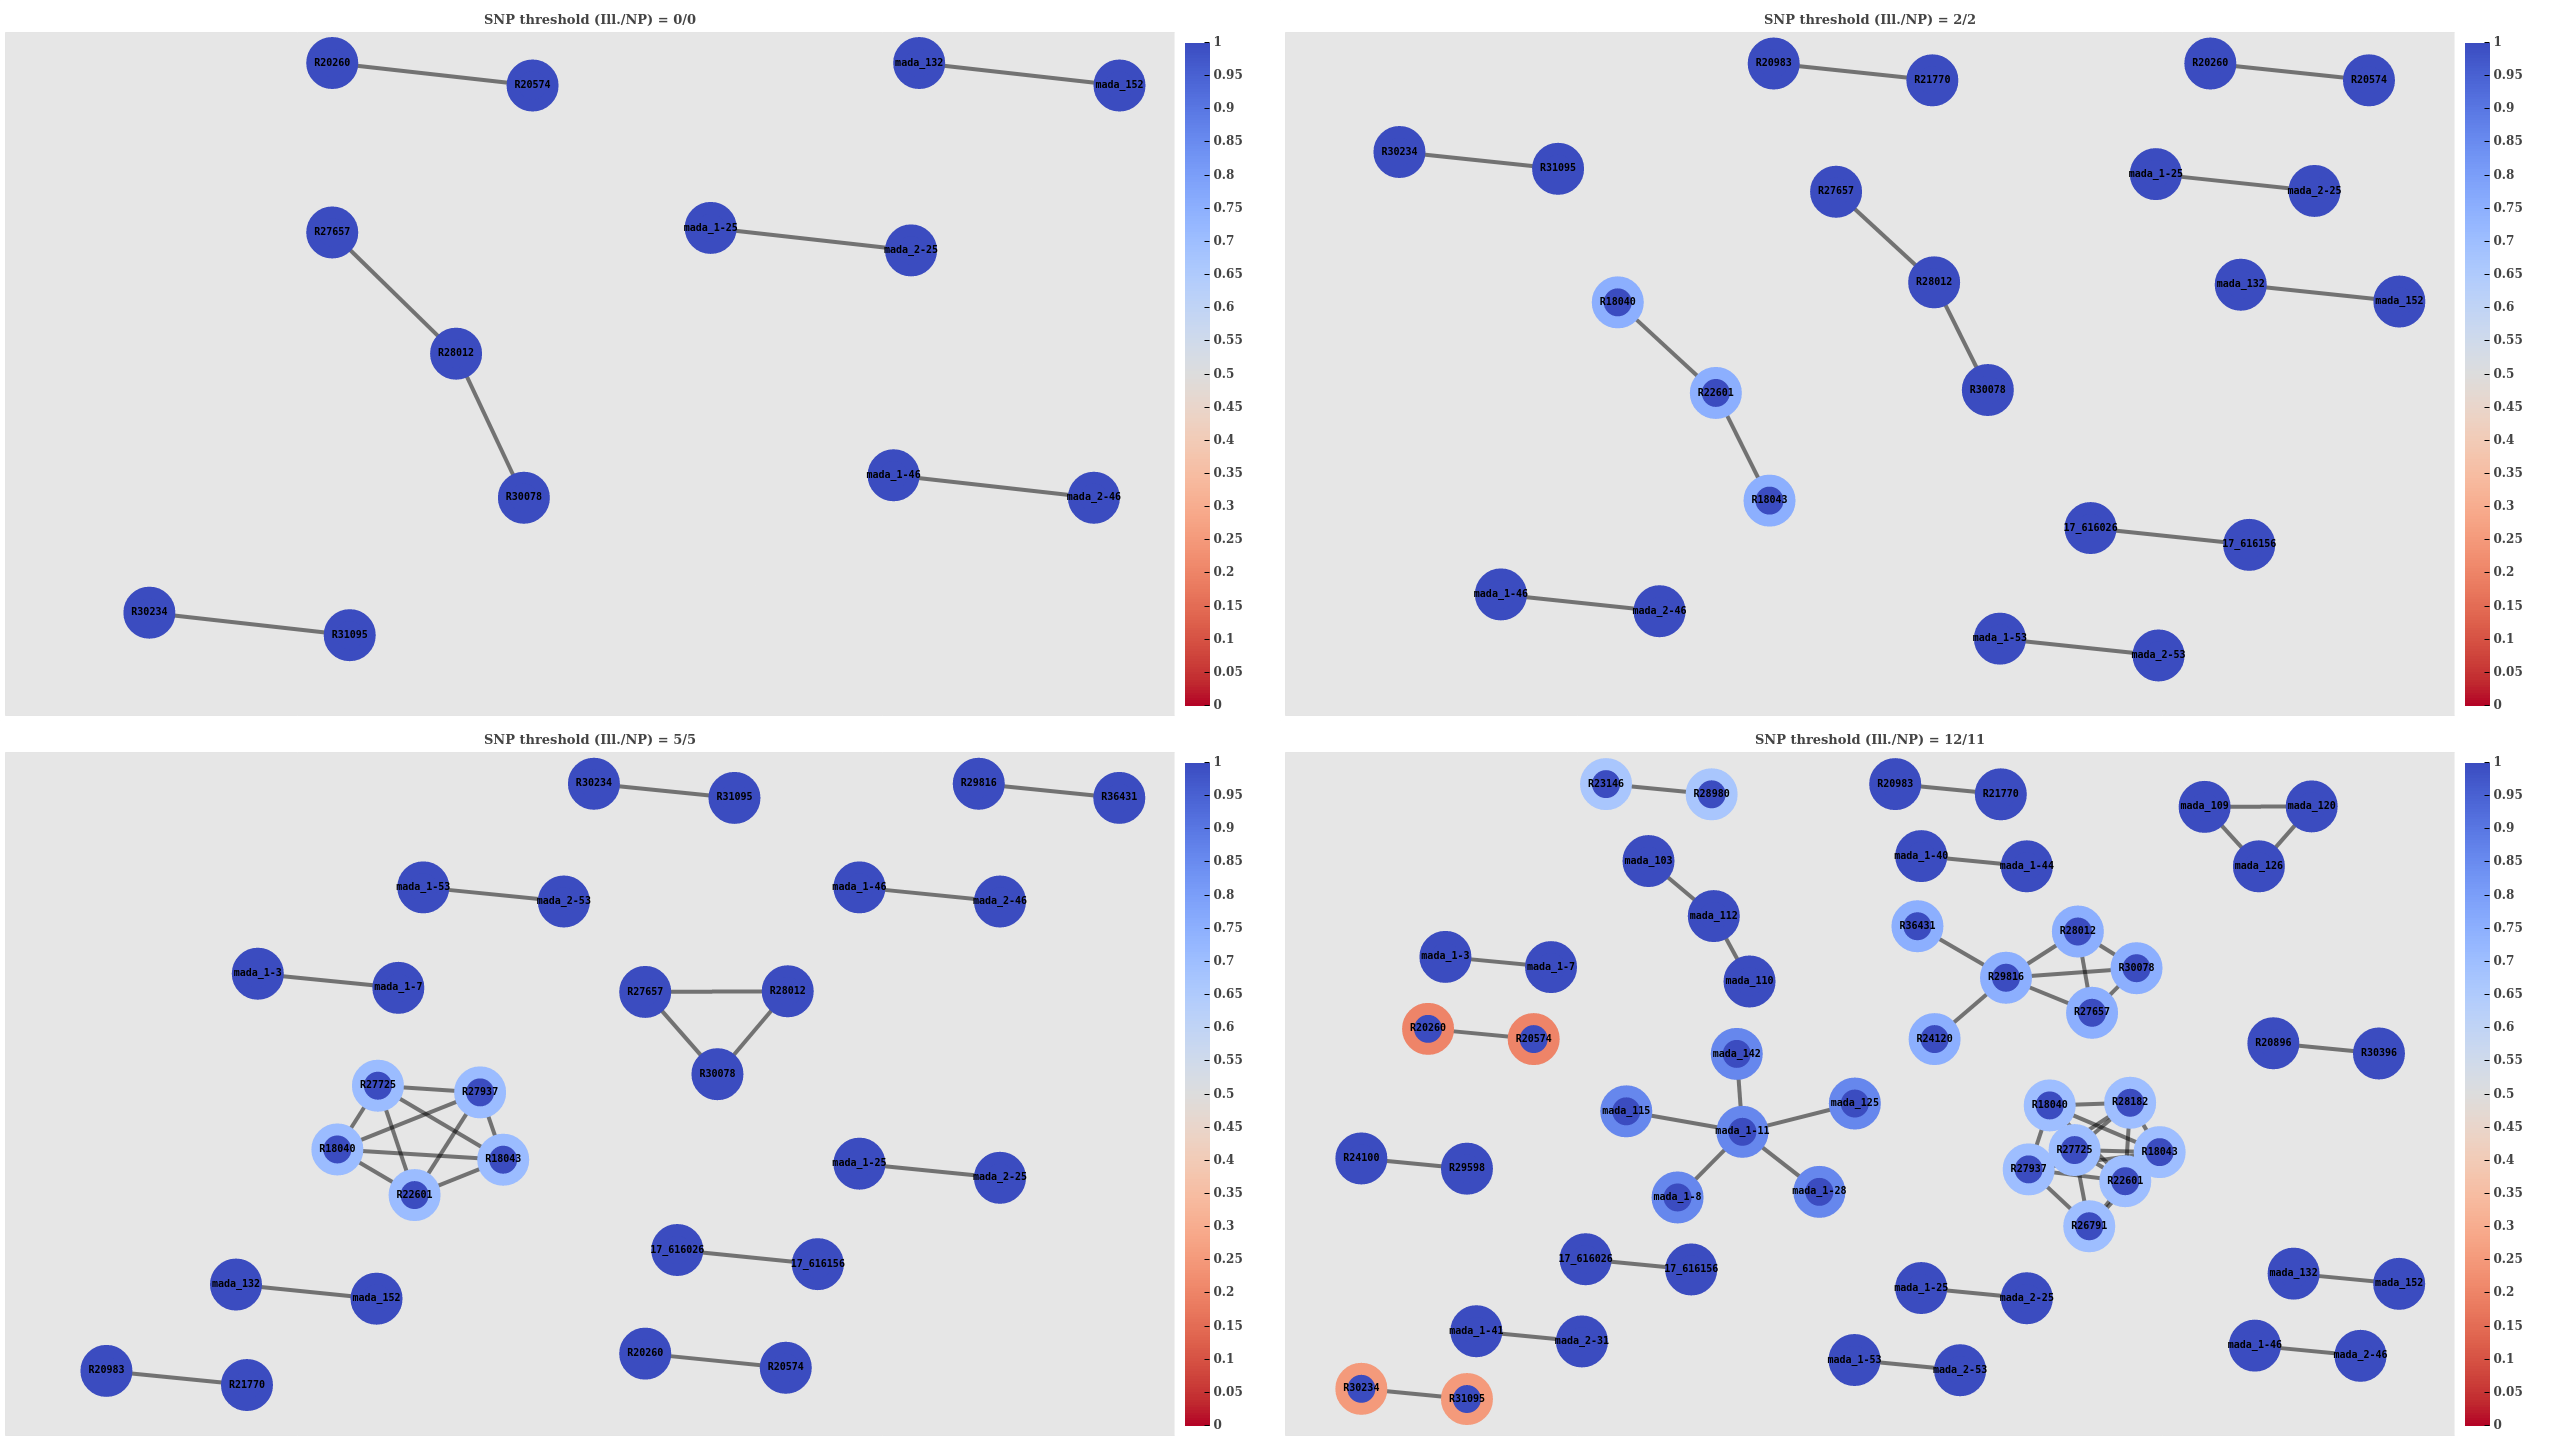
\includegraphics[width=0.90\columnwidth]{Chapter2/Figs/bcftools_clusters.png}
\caption{{Agreement of Illumina and bcftools (\ont{}) transmission clustering at SNP thresholds 0 (top-left), 2 (top-right), 5 (bottom-left) and 12 (bottom-right). The title of each subplot indicates the Illumina (Ill.) and \ont{} (NP) threshold used when clustering. Samples (nodes) are connected when the SNP distance between them is less than or equal to the relevant threshold. The inner and outer colours for each node indicates the SACR and SACP values, respectively, for the cluster it is a part of. The Illumina-based clustering is shown.
{\label{fig:bcftools-clusters}}
}}
\end{center}
\end{figure}

\begin{table}
\centering
\begin{tabular}{llll}
Threshold & SACR & SACP  & XCR           \\
\hline
0         & 1.0  & 1.0   & 0.015 (2/137) \\
\hline
2         & 1.0  & 0.966 & 0.008 (1/128) \\
\hline
5         & 1.0  & 0.949 & 0.057 (7/122) \\
\hline
12 (11)       & 1.0  & 0.845 & 0.031 (3/97) 
\end{tabular}
\caption{Summary of bcftools clustering metrics for four (Illumina) SNP distance thresholds. The threshold(s) in parentheses are the \ont{} equivalent threshold used. The fractions in parentheses for XCR indicate the underlying numbers. SACR=sample-averaged cluster recall; SACP=sample-averaged cluster precision; XCR=excess clustering rate.}
\label{tab:bcftools-cluster-summary}
\end{table}

\subsubsection{\pandora{} single-sample}

For \pandora{} single-sample we also chose to use the hand-picked SNP distance thresholds from analysis in \autoref{app:dist-sweep}. These are 16, 18, 18, and 27 for the Illumina thresholds of interest 0, 2, 5, and 12 respectively. The clustering results for each of these thresholds are summarised in \autoref{tab:map-cluster-summary} and visualised in \autoref{fig:map-clusters}. At no threshold was \pandora{} single-sample clustering able to achieve perfect SACR, SACP or XCR. In particular, all thresholds had a SACP value less than 0.69 and an XCR greater than 0.11. Taken together, these outline the fact that there were quite a lot of singletons that were erroneously clustered and many clusters joined. In large part, this is expected due to the much wider spread of distances along the y-axis for \pandora{} single-sample, in the inset of \autoref{fig:dotplot}, when compared to bcftools or \pandora{} multi-sample. Although the SACR values are not as low as the SACP, we place a higher value on them. The nodes with red(ish) outer circles in \autoref{fig:map-clusters} highlight clusters where samples have been missed. The actual clusters generated by \pandora{} single-sample can be seen in \autoref{fig:map-original-clusters}.

\begin{figure}
\begin{center}
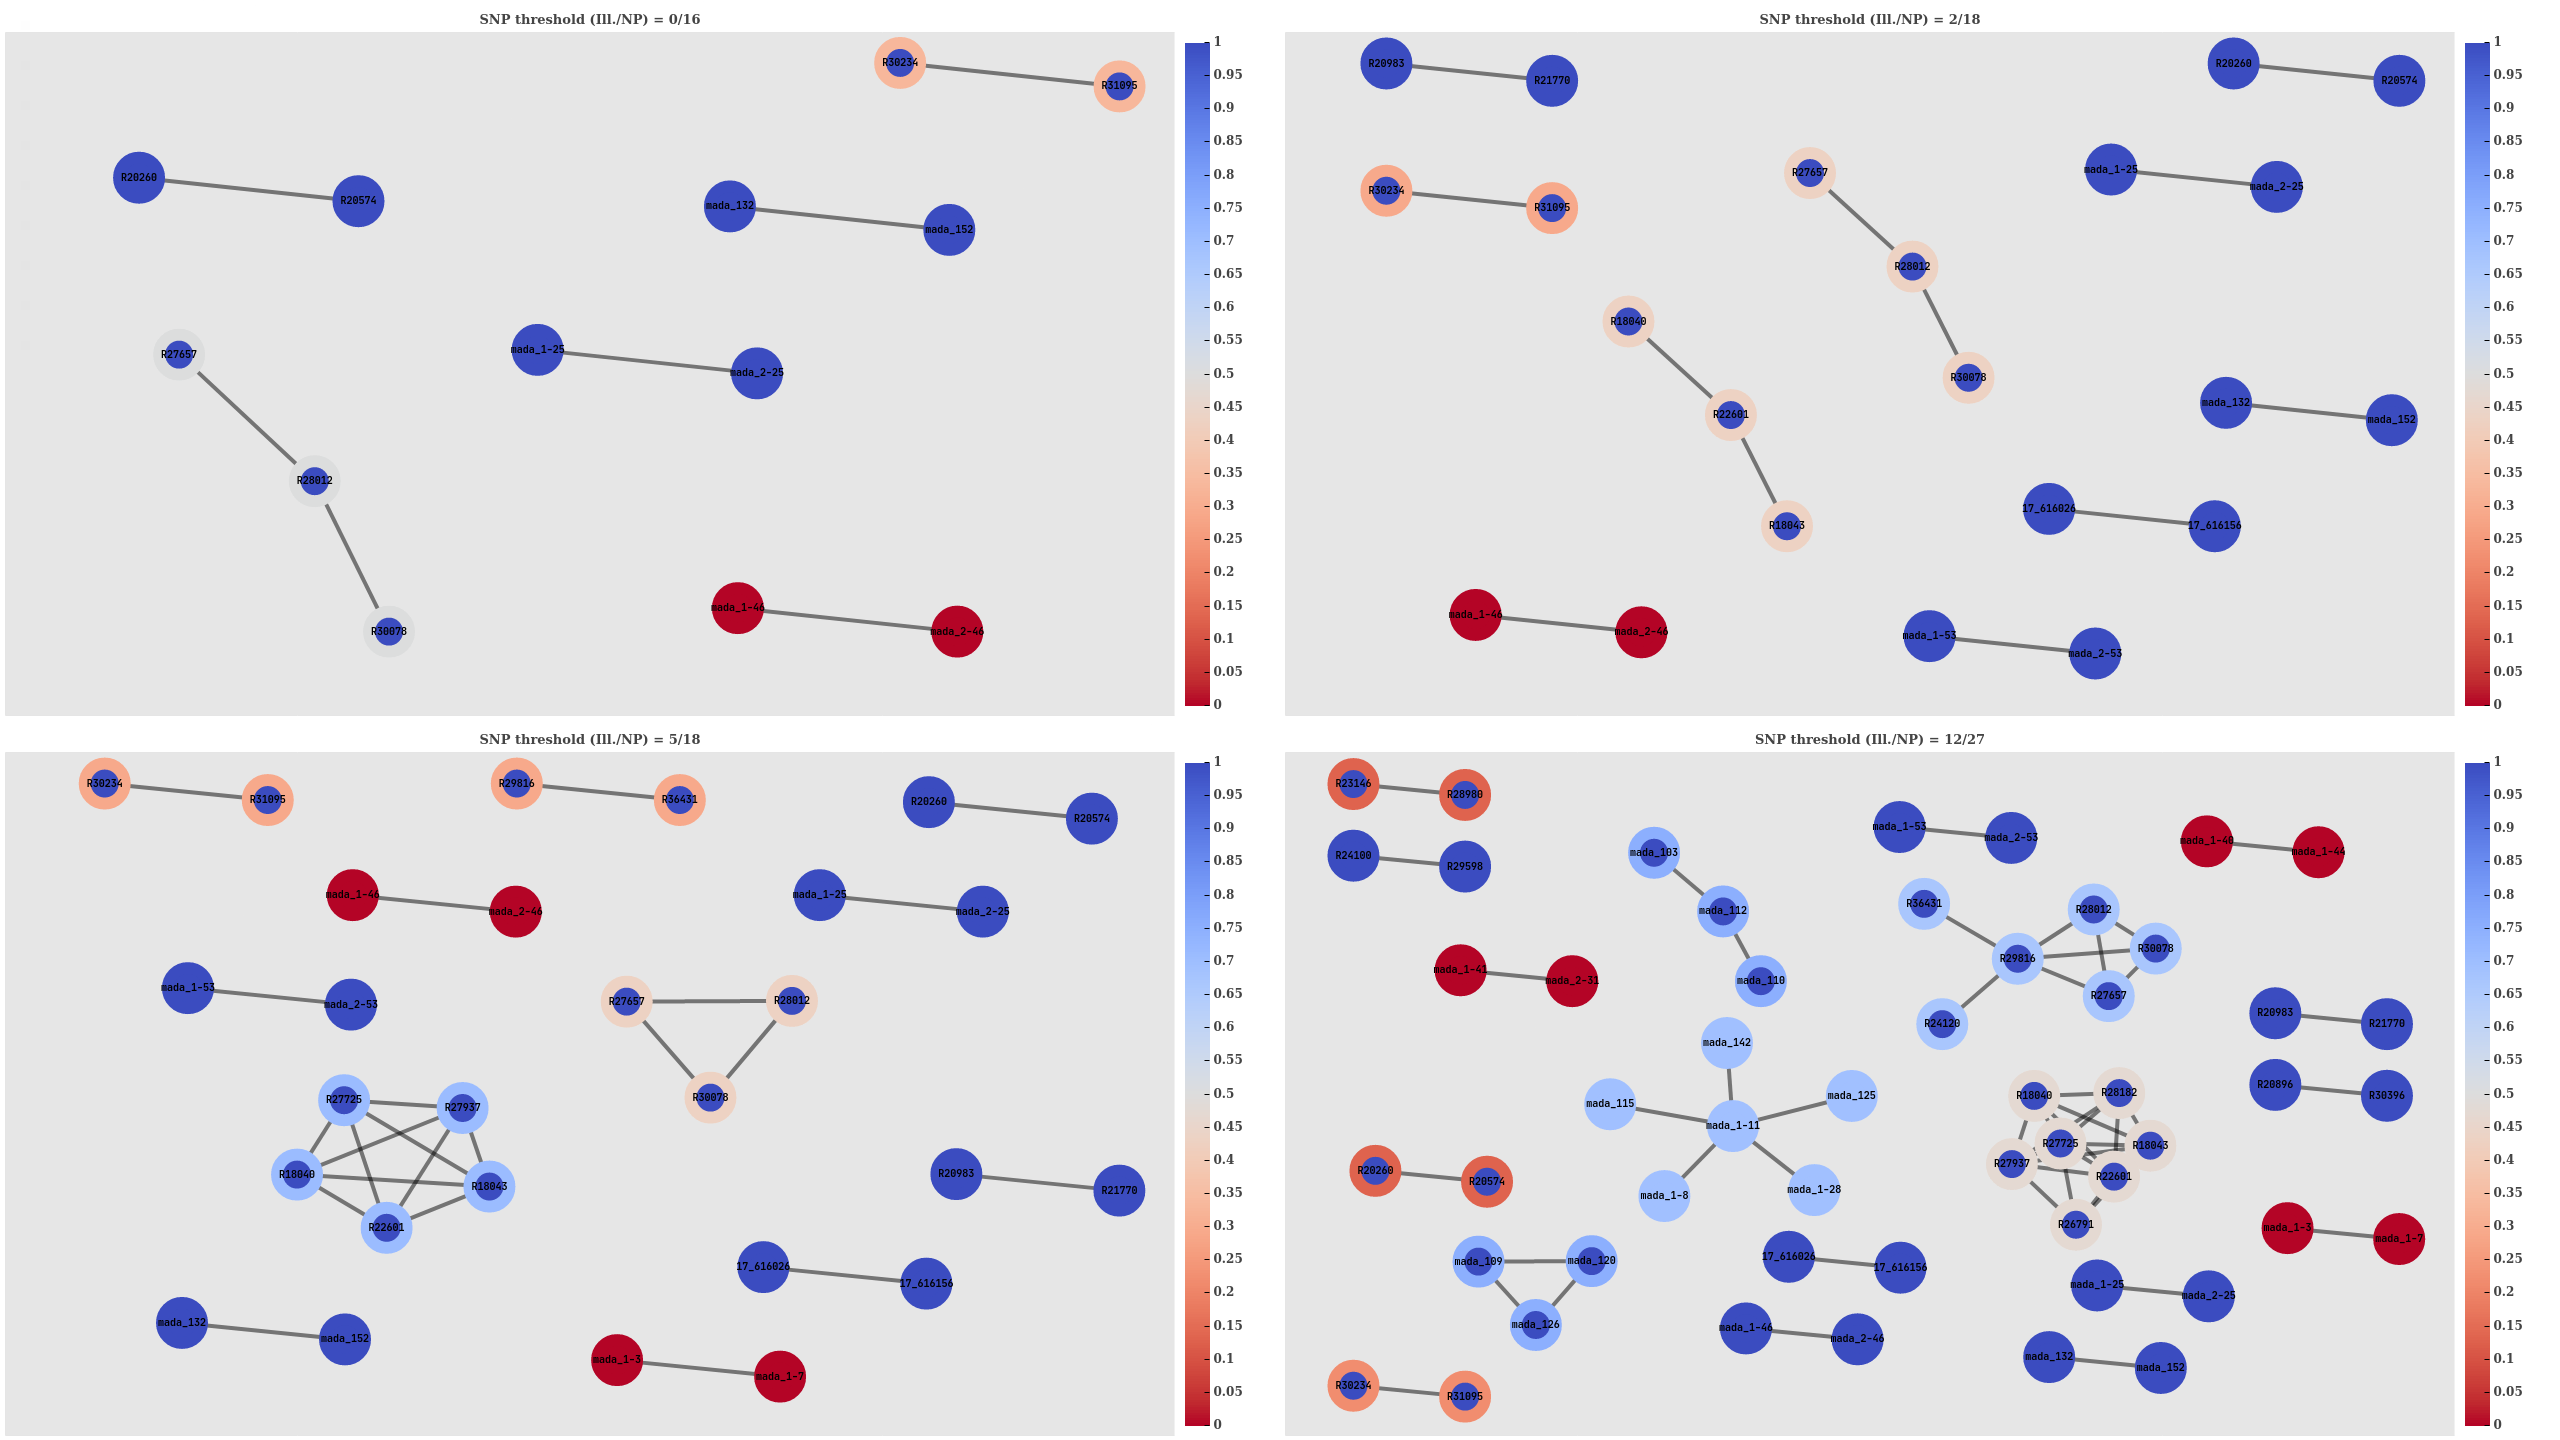
\includegraphics[width=0.90\columnwidth]{Chapter2/Figs/pandora_map_clusters.png}
\caption{{Agreement of Illumina and \pandora{} single-sample (\ont{}) transmission clustering at SNP thresholds 0 (top-left), 2 (top-right), 5 (bottom-left) and 12 (bottom-right). The title of each subplot indicates the Illumina (Ill.) and \ont{} (NP) threshold used when clustering. Samples (nodes) are connected when the SNP distance between them is less than or equal to the relevant threshold. The inner and outer colours for each node indicates the SACR and SACP values, respectively, for the cluster it is a part of. The Illumina-based clustering is shown.
{\label{fig:map-clusters}}%
}}
\end{center}
\end{figure}

\begin{table}
\centering
\begin{tabular}{llll}
Threshold & SACR  & SACP  & XCR            \\
\hline
0 (16)    & 0.846 & 0.628 & 0.146 (20/137) \\
\hline
2 (18)    & 0.909 & 0.688 & 0.141 (18/128) \\
\hline
5 (18)    & 0.857 & 0.643 & 0.115 (11/122) \\
\hline
12 (27)   & 0.852 & 0.621 & 0.124 (12/97)  
\end{tabular}
\caption{Summary of \pandora{} single-sample clustering metrics for four (Illumina) SNP distance thresholds. The threshold(s) in parentheses are the \ont{} equivalent threshold used. The fractions in parentheses for XCR indicate the underlying numbers. SACR=sample-averaged cluster recall; SACP=sample-averaged cluster precision; XCR=excess clustering rate.}
\label{tab:map-cluster-summary}
\end{table}

\subsubsection{\pandora{} multi-sample}

The SNP thresholds we use for \pandora{} multi-sample clustering are 0, 1, 3, and 7. The results of this clustering are summarised in \autoref{tab:compare-cluster-summary} and visualised in \autoref{fig:compare-clusters}. One important result is that unlike the single-sample approach of \pandora{}, the multi-sample mode leads to perfect SACR across all thresholds. Additionally, the clustering at the threshold of 0 perfectly mirrors Illumina. At a threshold of 2, there was one singleton added to an otherwise perfect cluster and 2 additional clusters of size 2. At thresholds 5 and 12 there were a number of clusters joined into larger ones and some additions of singletons to existing clusters, along with new clusters. The actual clusters produced by \pandora{} multi-sample can be seen in \autoref{fig:compare-original-clusters}.

\begin{figure}
\begin{center}
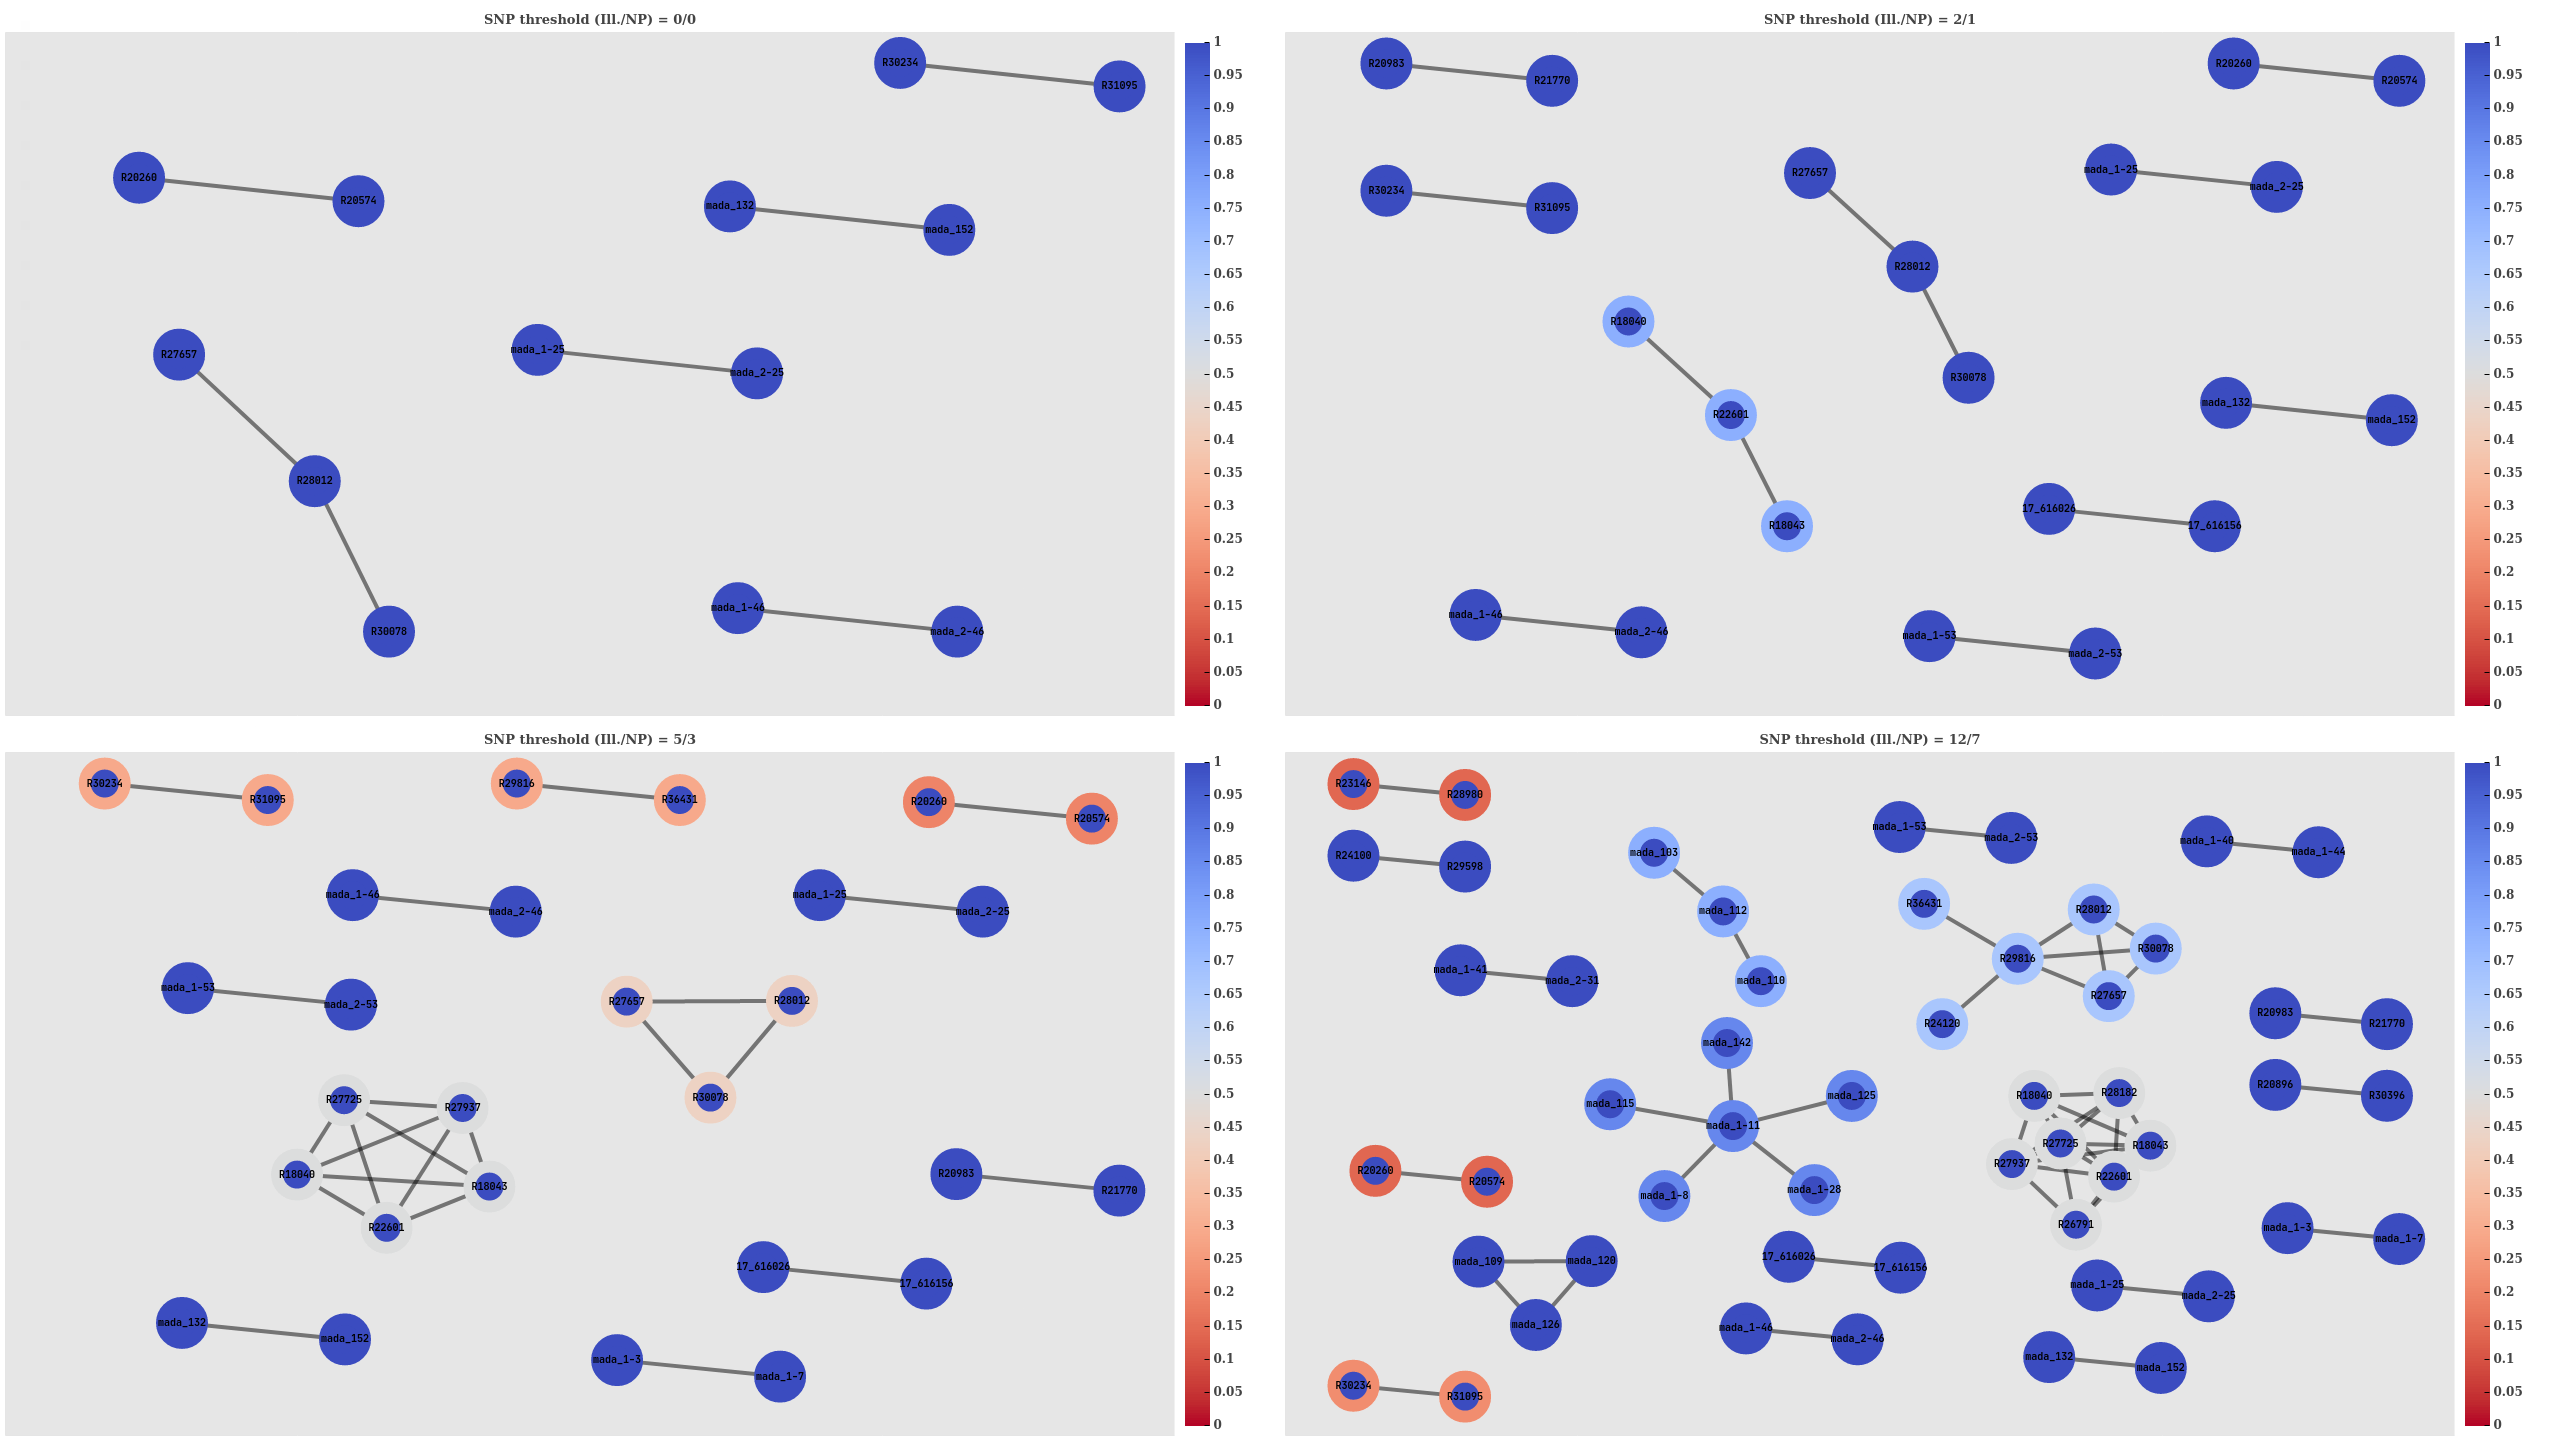
\includegraphics[width=0.90\columnwidth]{Chapter2/Figs/pandora_compare_clusters.png}
\caption{{Agreement of Illumina and \pandora{} multi-sample (\ont{}) transmission clustering at SNP thresholds 0 (top-left), 2 (top-right), 5 (bottom-left) and 12 (bottom-right). The title of each subplot indicates the Illumina (Ill.) and \ont{} (NP) threshold used when clustering. Samples (nodes) are connected when the SNP distance between them is less than or equal to the relevant threshold. The inner and outer colours for each node indicates the SACR and SACP values, respectively, for the cluster it is a part of. The Illumina-based clustering is shown.
{\label{fig:compare-clusters}}%
}}
\end{center}
\end{figure}

\begin{table}
\centering
\begin{tabular}{llll}
Threshold & SACR  & SACP  & XCR            \\
\hline
0        & 1.0 & 1.0 & 0.0 (0/137) \\
\hline
2 (1)    & 1.0 & 0.966 & 0.039 (5/128) \\
\hline
5 (3)    & 1.0 & 0.690 & 0.090 (11/122) \\
\hline
12 (7)   & 1.0 & 0.772 & 0.103 (10/97)  
\end{tabular}
\caption{Summary of \pandora{} multi-sample clustering metrics for four (Illumina) SNP distance thresholds. The threshold(s) in parentheses are the \ont{} equivalent threshold used. The fractions in parentheses for XCR indicate the underlying numbers. SACR=sample-averaged cluster recall; SACP=sample-averaged cluster precision; XCR=excess clustering rate.}
\label{tab:compare-cluster-summary}
\end{table}

\subsection{Summary}
\label{sec:cluster-summary}

The results presented in this section show that when using bcftools for variant calling \ont{} is capable of producing transmission clusters with a high degree of similarity to Illumina. Most importantly, no samples deemed part of a cluster by Illumina were missed by bcftools. We have also shown that the Illumina SNP thresholds of 0, 2, and 5 are also valid for \ont{} variant calls from bcftools and the threshold of 12 needs only to be reduced to 11. 

We also investigated whether the genome graph method of \pandora{} could be used to produce accurate transmission clusters. While the single-sample approach did not yield particularly good results, the multi-sample mode shows promise. For all SNP thresholds assessed, \pandora{}'s multi-sample method did not miss any samples from clustering. The SACP values for thresholds 0 and 2 were as good as those from bcftools, but at thresholds 5 and 12 \pandora{} did not perform as well. 

%=========================================================================

\section{Transmission clusters with mixed Illumina and \ont{} data}

Having established that Illumina-defined transmission clusters can be confidently recreated with \ont{} data, we turn to the question of whether the same holds true when mixing Illumina and \ont{} data. Being able to deduce transmission clusters from a mixture of sequencing modalities would allow greater integration across datasets from various sources and prevent laboratories from being locked into any one sequencing technology. As the uptake of \ont{} sequencing increases it seems inevitable there will be cases where comparisons between these sequencing modalities is necessary. To address this question we simulate varying degrees of \ont{}/Illumina mixtures and look at how this impacts clustering. To this end, we investigate what the impact (if any) of combining Illumina and \ont{} datasets has on SACR, SACP and XCR (see \autoref{sec:cluster-similarity} for definitions). For the \ont{} data, we use the bcftools distance matrices as they were shown to be the most concordant with Illumina (\autoref{sec:cluster-summary}).

Firstly, we get a sense for how comparable the distances are likely to be but looking at the "self-distance" for each sample - the distance between a sample's Illumina and \ont{} data.  As the sequencing data originates from the same source, we know the self-distance for any sample \emph{should} be 0. However, we also know there are major technological differences between Illumina and \ont{}, so small variability in self-distance is likely. We plot these self-distances in \autoref{fig:self-dist} and see that 64\% (96/150) of the samples have a distance of 0 between their Illumina (COMPASS) and \ont{} (bcftools) data, with 84\% (126/150) less than 2 SNPs apart. All samples have a self-distance less than 9, with the exception of one sample (\vrb{mada\_1-33}), which has a self-distance of 53. We investigated the possibility of a sample mix-up being the cause of this discrepancy but were unable to find any such convincing evidence. 

\begin{figure}
\begin{center}
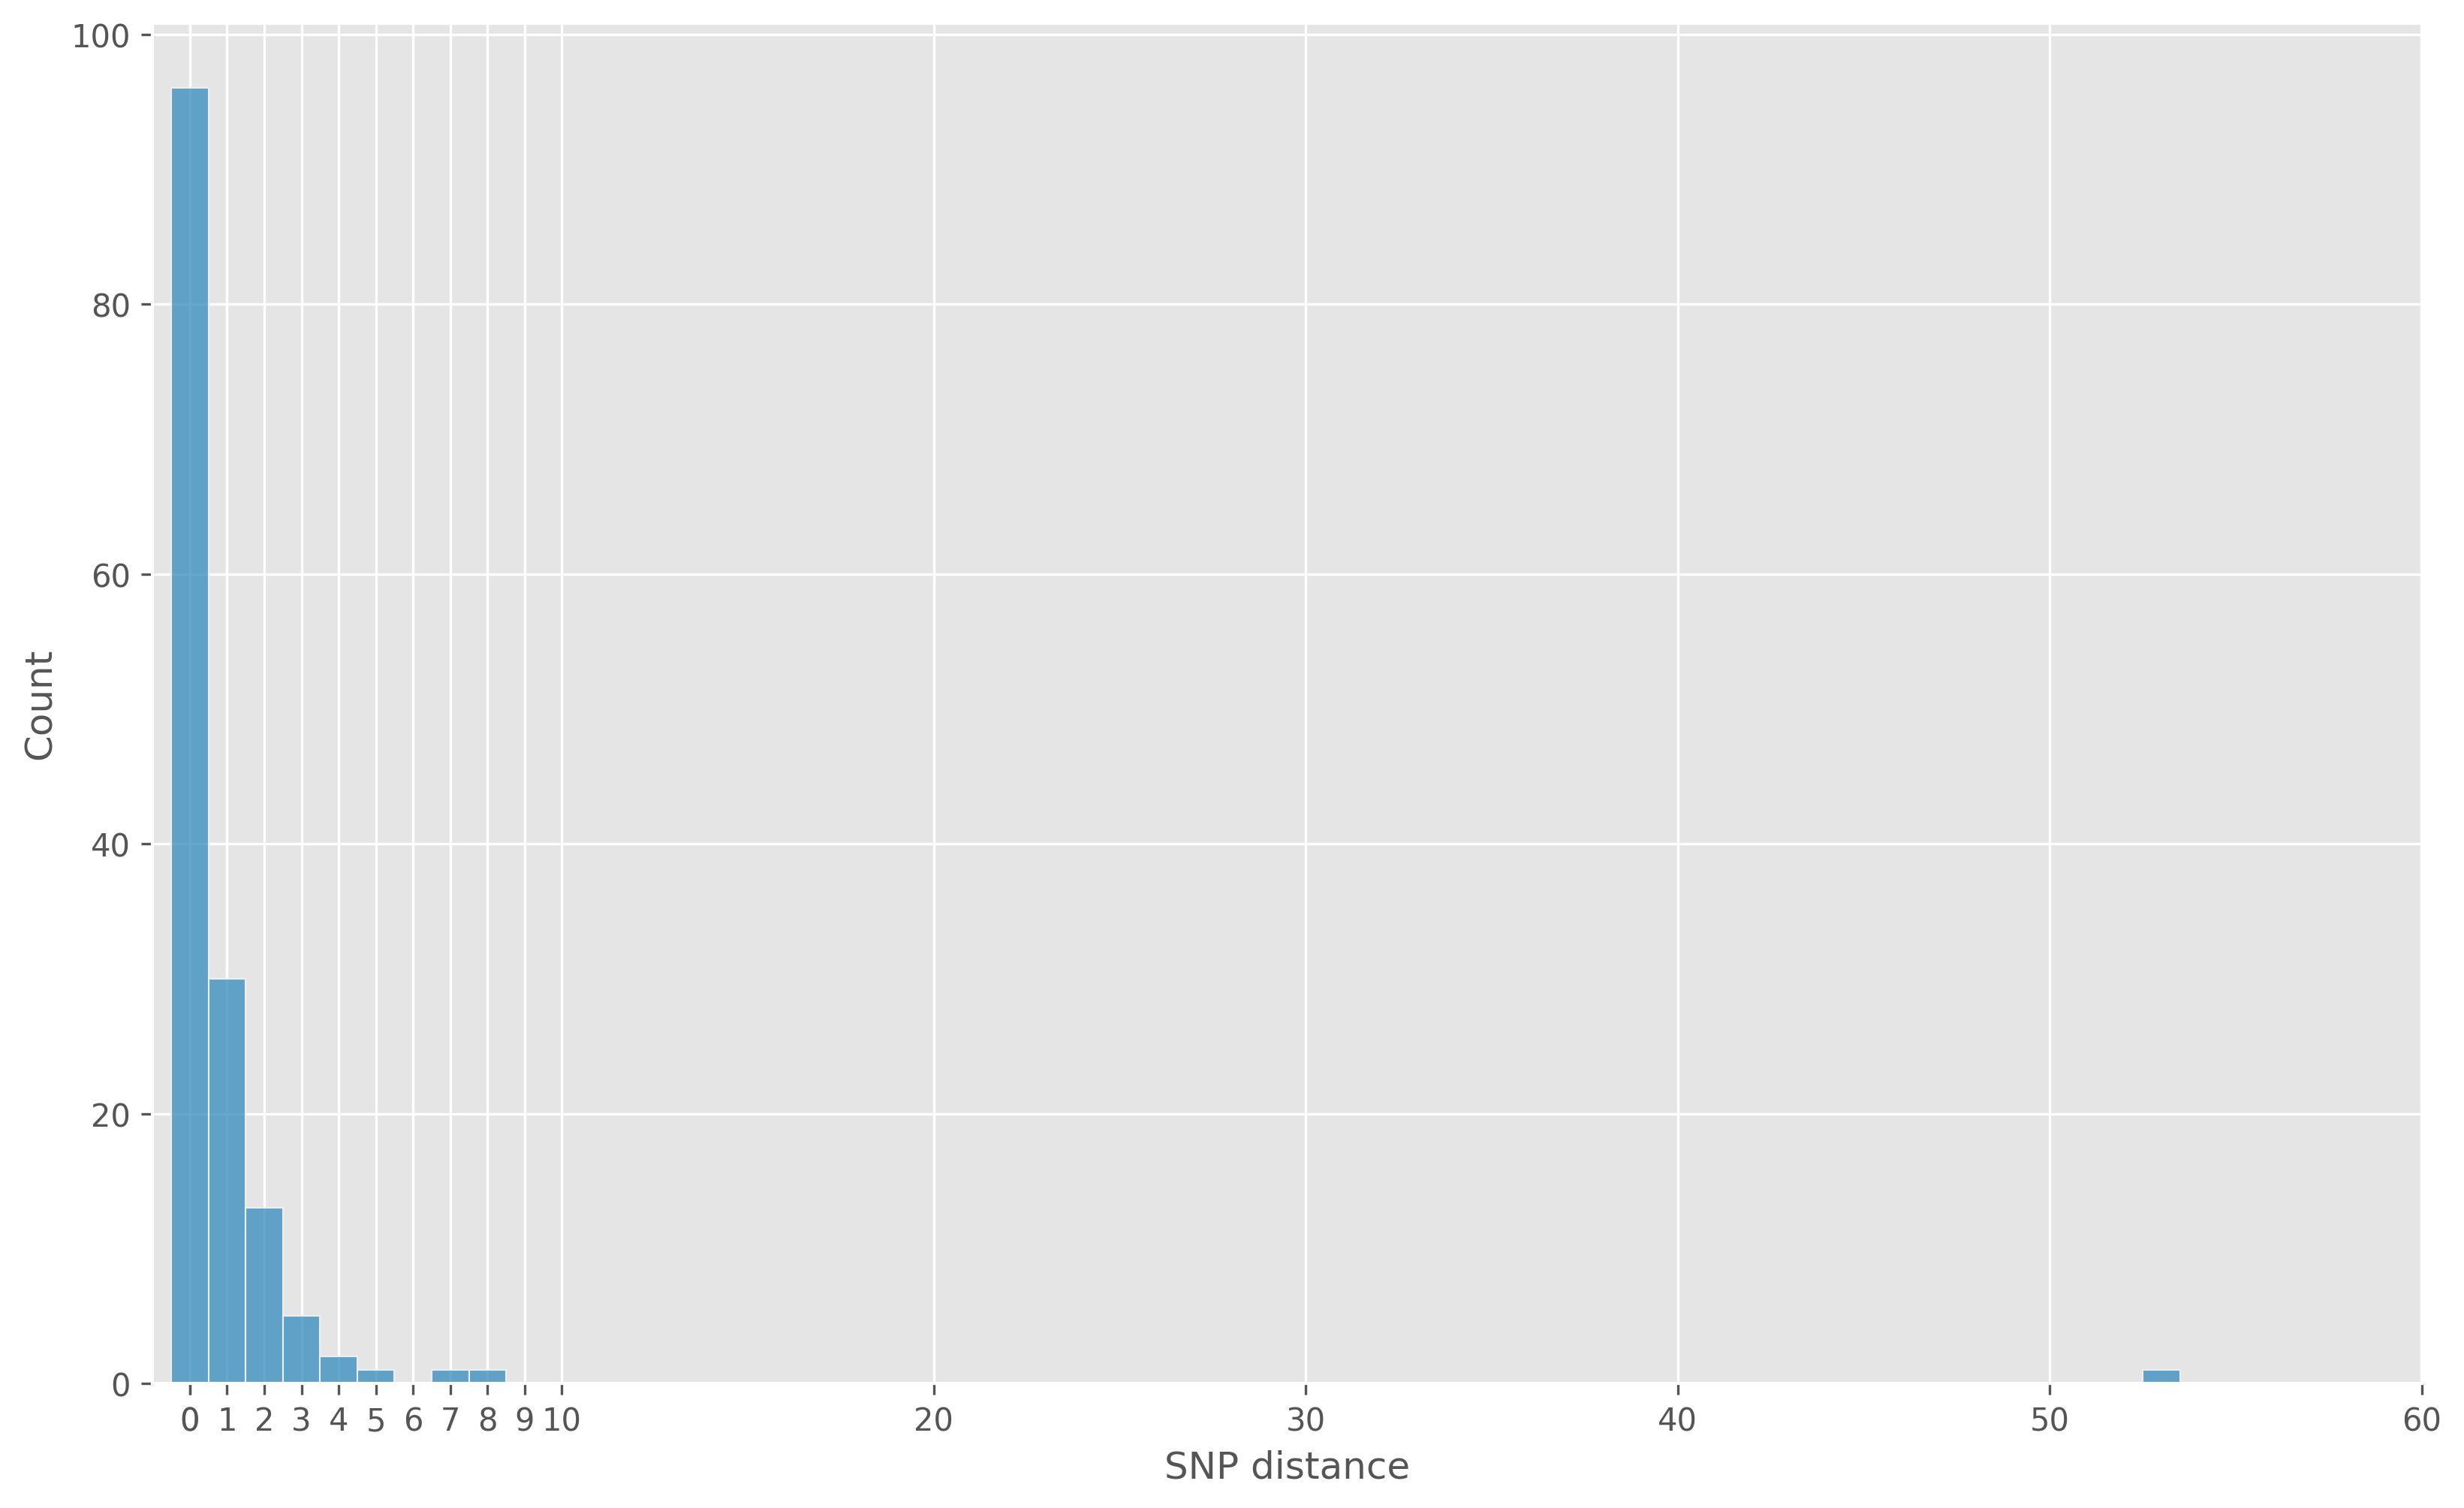
\includegraphics[width=0.90\columnwidth]{Chapter2/Figs/mixed_self_dist.png}
\caption{{Mixed modality "self-distance". This plot shows the SNP distance (x-axis) between each sample's COMPASS (Illumina) and bcftools (\ont{}) VCF calls.
\label{fig:self-dist}
}}
\end{center}
\end{figure}

Next, we look at the pairwise SNP distance relationship, akin to that in \autoref{sec:snp-dist}. \autoref{fig:mixed-dotplot} shows the mixed SNP distances have a similar relationship to the single-technology correlation in \autoref{fig:dotplot}. The difference here, however, is that the y-axis represents the distance between one sample's Illumina data and the other's \ont{}. There are twice as many data points in this plot though as the distance between two samples is not necessarily reciprocal for mixed modality distances (as we saw with the self-distances). That is, for two samples $a$ and $b$, $distance(a_I,b_N) \neq distance(a_N, b_I)$, where $I$ and $N$ refer to Illumina and \ont{} data respectively. 

In the zoomed inset window of \autoref{fig:mixed-dotplot}, there is a cluster of outlying points with a higher mixed distance than Illumina distance. All of these points relate to combinations of 6 samples in particular. These were investigated for evidence of a sample swap or poor quality data, but nothing was found to support such a claim. In reality, it just seems the \ont{} data for some of the samples is quite different to the Illumina data of the other samples.

\begin{figure}
\begin{center}
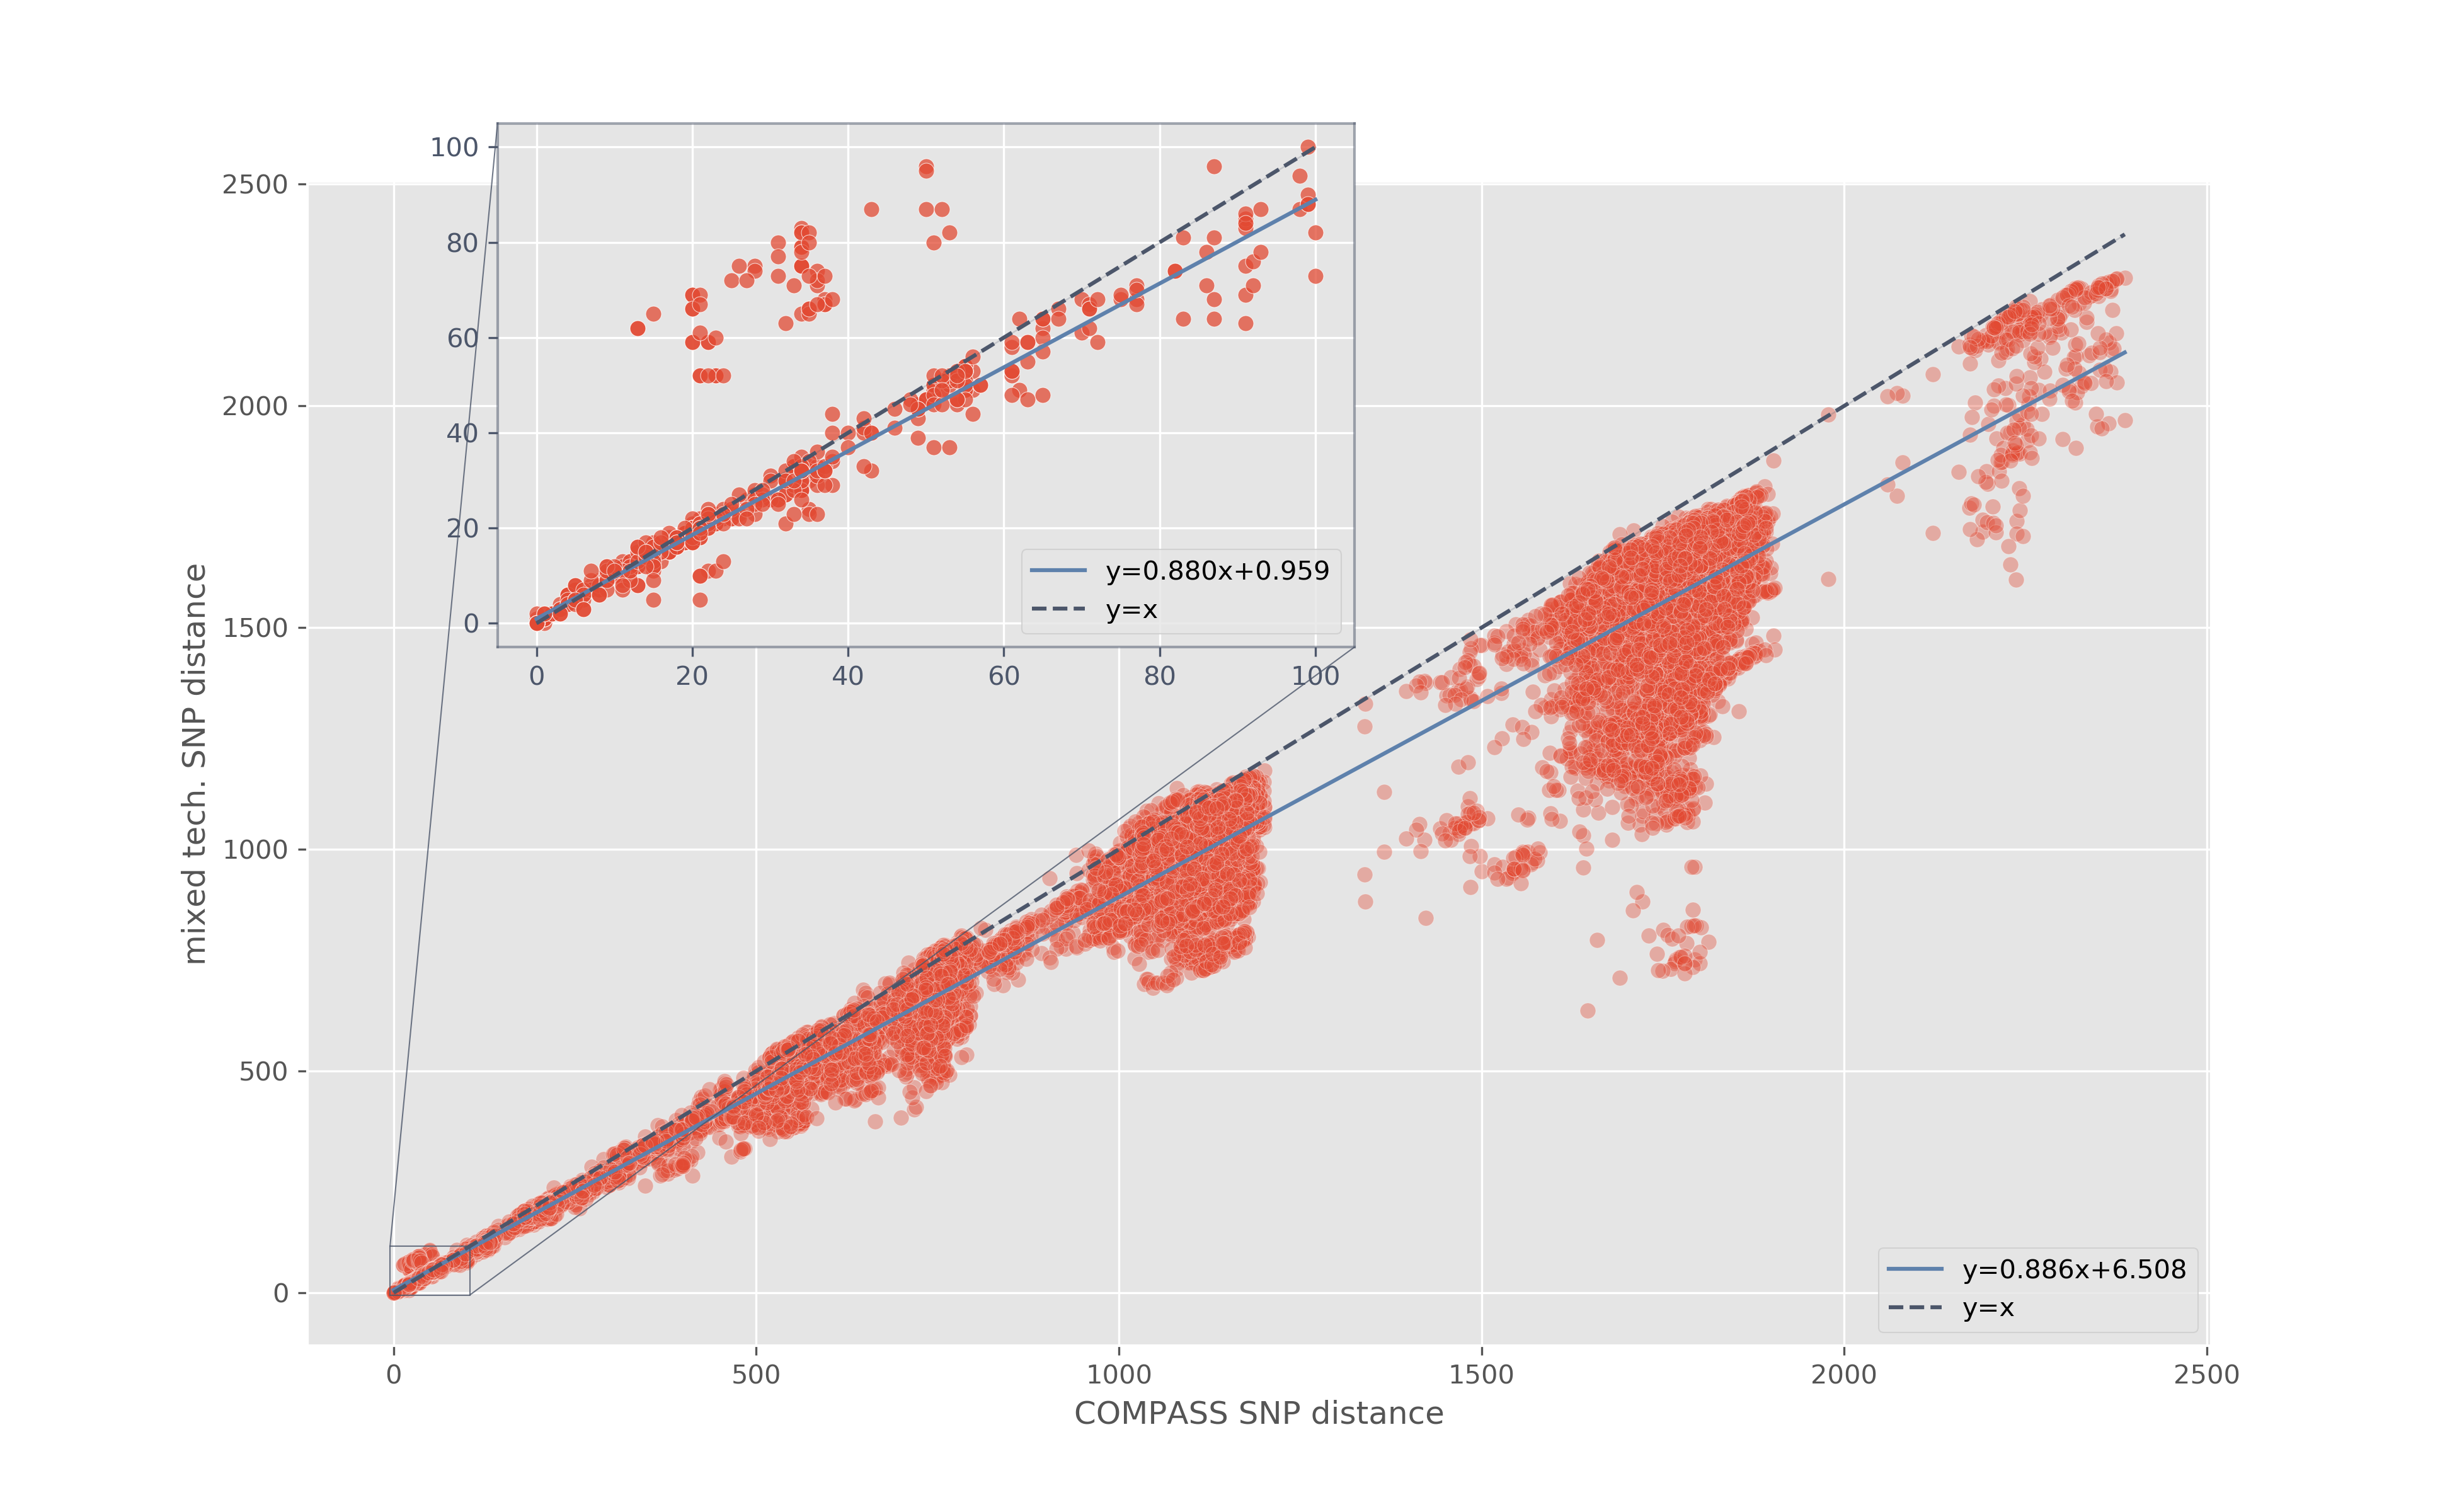
\includegraphics[width=0.90\columnwidth]{Chapter2/Figs/mixed-dotplot.png}
\caption{{The relationship of the distance between all pairs of samples based on Illumina (COMPASS) VCF calls (X-axis) and mixed COMPASS-bcftools calls (Y-axis). The black, dashed line indicates the relationship we would expect if the distance between a pair of samples were the same for both approaches. The blue line indicates the line of best fit based on fitting a robust linear regression model to the data. The inset gives a closer look at the relationship for all sample pairs where the COMPASS distance is less than or equal to 100 SNPs. The legend indicates the linear equations for the lines. Note: to prevent model skew, we do not include self-distance pairs.
{\label{fig:mixed-dotplot}}
}}
\end{center}
\end{figure}

We now examine transmission clusters for mixtures of \ont{} and Illumina data using the same SNP thresholds used in \autoref{sec:clustering}. The SNP threshold we use when comparing different modalities is the Illumina SNP thresholds. The mixture ratios we investigate are 0.01, 0.05, 0.1, 0.25, 0.5, 0.75, and 0.9. That is, for a ratio of 0.25, we \emph{randomly} allocate 25\% of the samples to \ont{} and the remainder to Illumina. For each SNP threshold and ratio, we calculate the XCR, SACR and SACP that the clustering produces. We repeat this process 1000 times for each threshold and ratio to simulate different mixtures of sample/technology pairs. The simulation of so many different mixed pairs is intended to provide insight into how robust clustering with mixtures of sequencing datasets is likely to be.  

The results of these simulations are shown in \autoref{fig:mixed-sims}. We found that for all SNP thresholds and ratios, the median SACR was 1.0. In other words, regardless of the \ont{}/Illumina mixture ratio, for all thresholds we used, no sample is missed from its expected clustering - on average. The SACP values decrease somewhat as the \ont{}ratio increases. However, the lowest median SACP value was 0.845 (threshold 12, ratio 0.9), which is also the SACP value obtained for the \ont{}-only clustering in \autoref{sec:bcftools-clustering} with the same threshold. The XCR values tend to increase slightly as more \ont{} samples are added. In the most extreme case, 0.057 was the highest XCR value in any simulation (SNP threshold 5). Incidentally, this is the same as the XCR obtained for the \ont{}-only clustering of the same SNP threshold, which equates to 7 of the 122 non-clustered samples being clustered. However, regardless of the XCR, no samples that should have been clustered were missed (on average).

\begin{figure}
\begin{center}
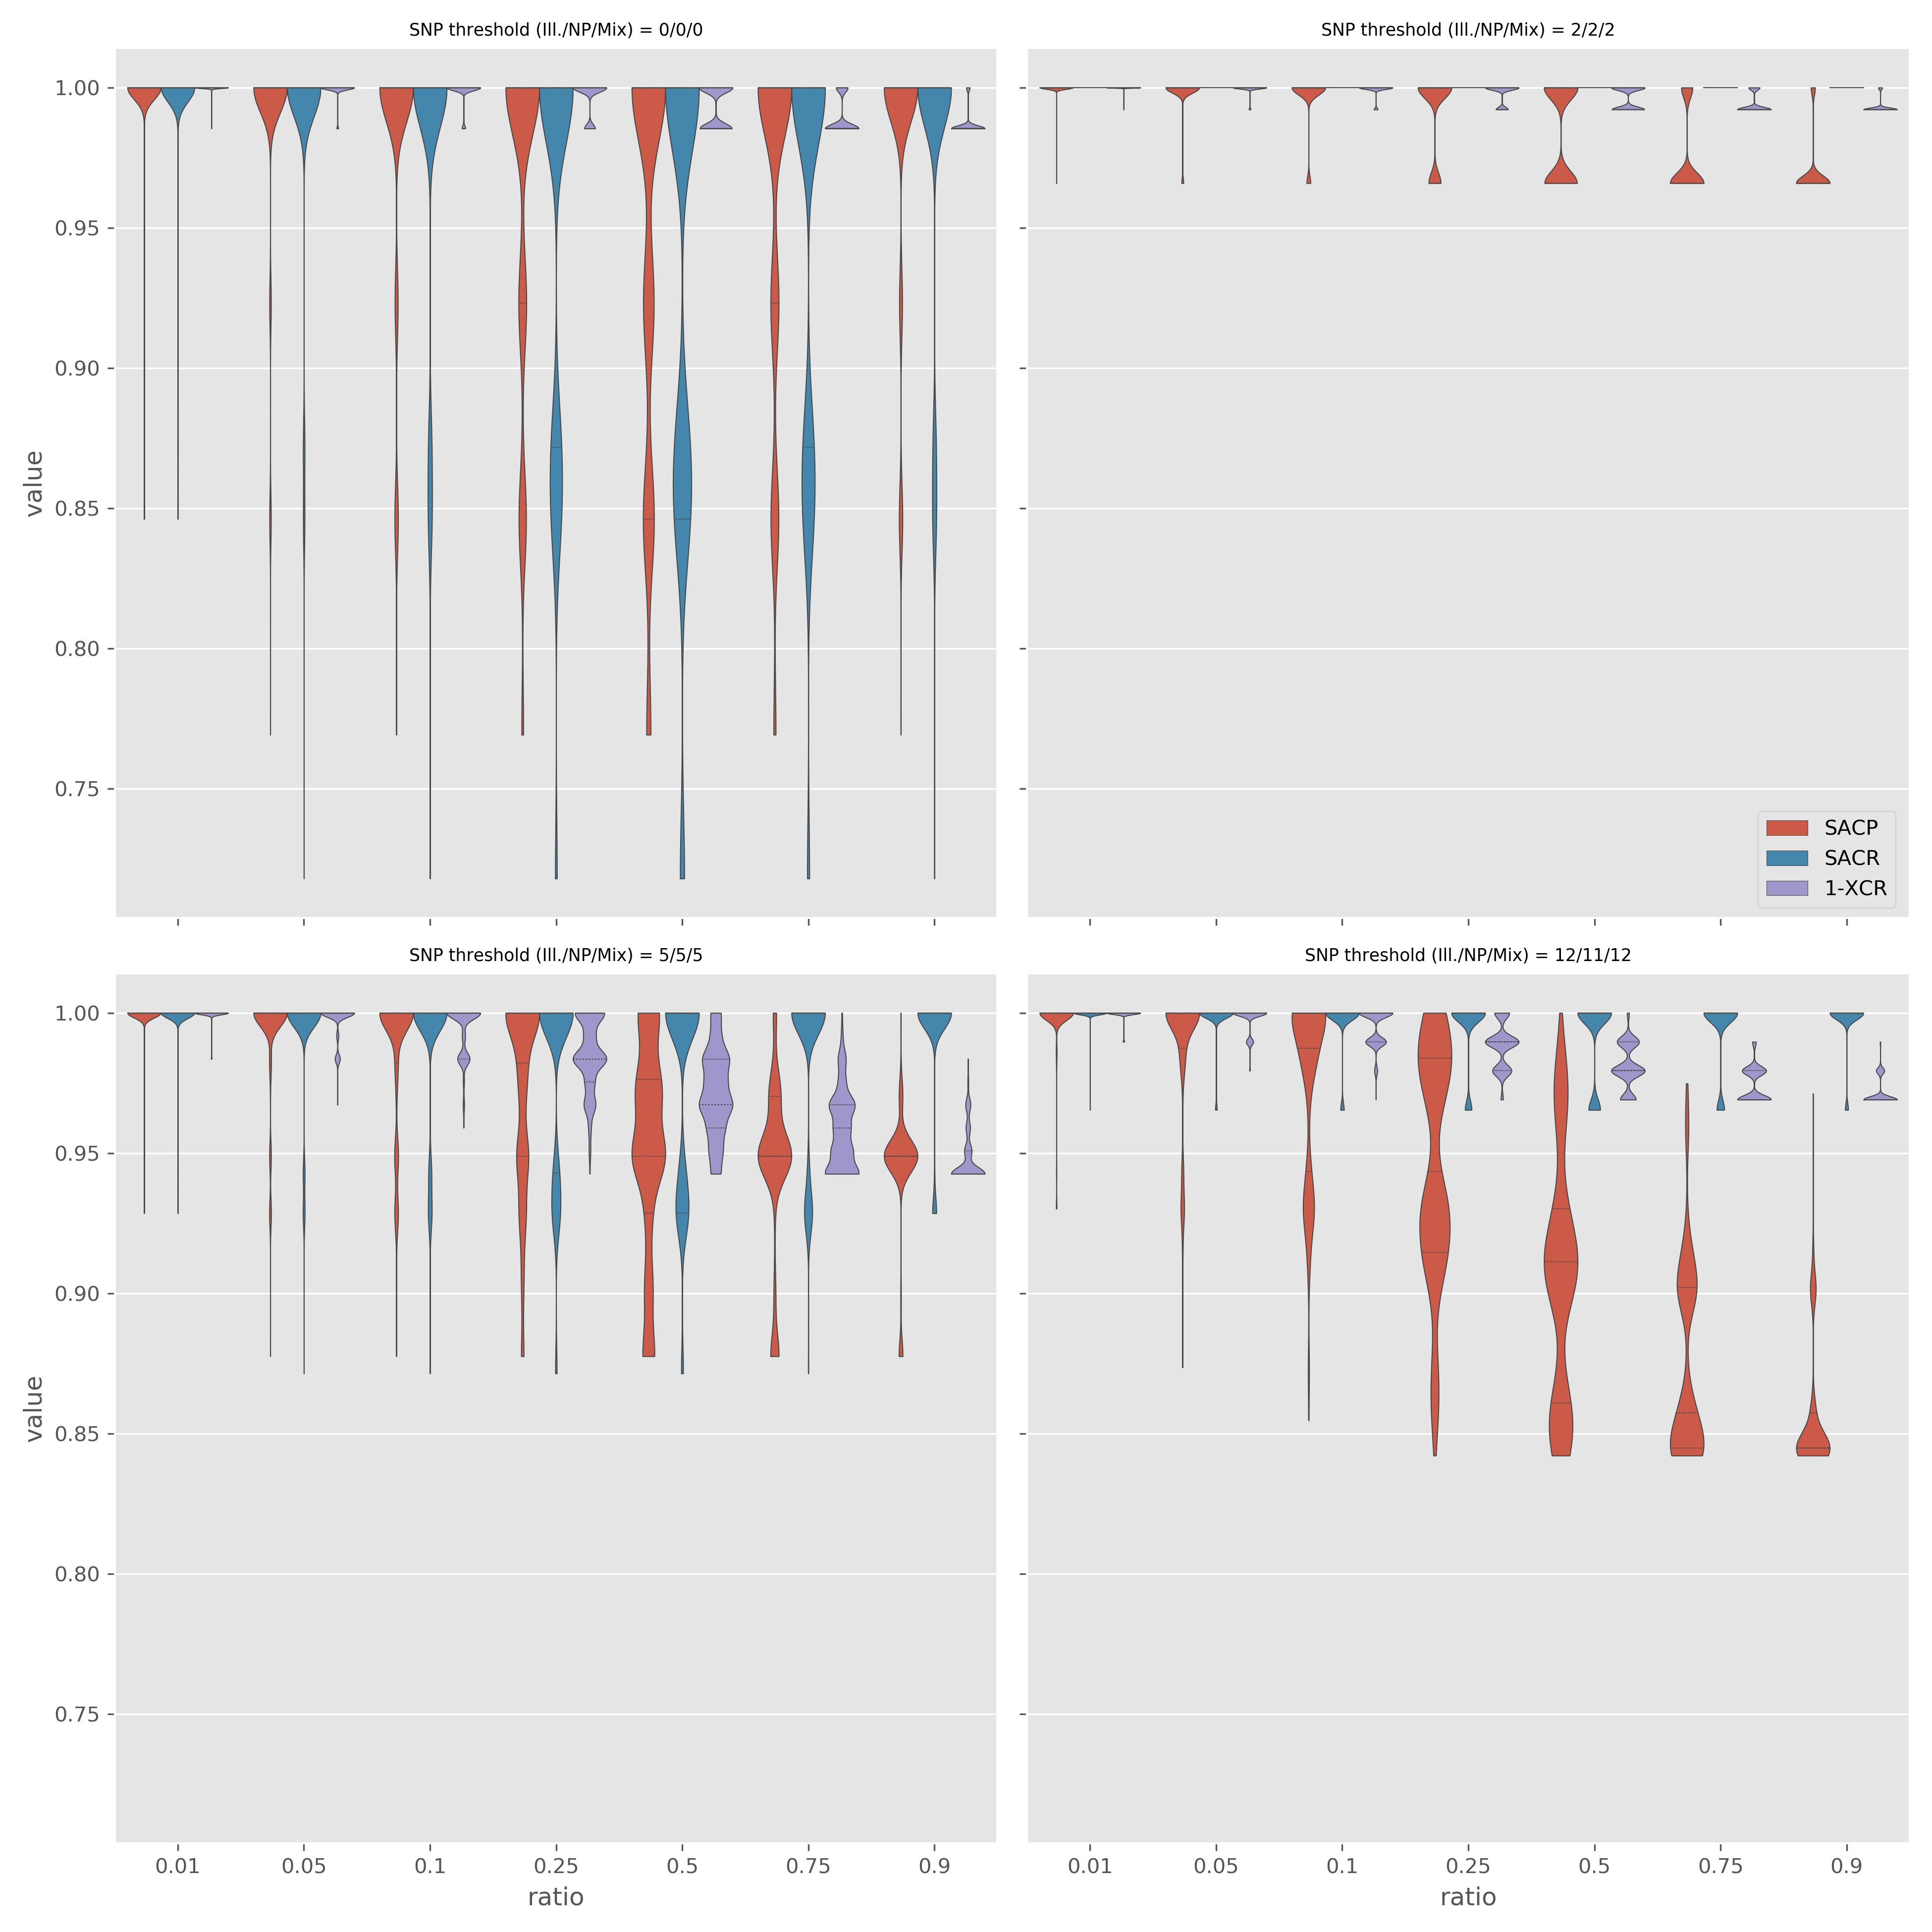
\includegraphics[width=0.90\columnwidth]{Chapter2/Figs/mixed_simulations.png}
\caption{{Simulating varying ratios (X-axis) of \ont{}/Illumina sample mixtures. The different thresholds (subplots) indicate the cutoff for defining samples as part of a cluster. The Y-axis depicts the Sample-Averaged Cluster Precision and Recall (SACP/SACR) and Excess Clustering Rate (XCR) distributions over all simulation runs (XCR is shown as (1-XCR) for better axis-scaling). For each ratio/threshold combination we run 1000 simulations where the \ont{} and Illumina data is randomly split into the relevant ratio and clusters are defined based on the relevant threshold. The titles for each subplot indicate the SNP threshold used when comparing Illumina (Ill.), \ont{} (NP), or mixed-technology sample pairs.
{\label{fig:mixed-sims}}%
}}
\end{center}
\end{figure}

\subsection{Summary}

In this section we have shown that putative transmission clusters constructed using mixtures of Illumina and \ont{} data are consistent with those produced by Illumina data alone.

%=========================================================================

\section{Discussion}


Recent work from CITE \etal{} is the first effort to assess \ont{} for the clustering of \mtb{} samples based on genetic distance. While their work had a larger number of samples to ours (431), the SNP distance comparison details were very brief and were only presented for a subset of 14 samples. They present the results as a distance matrix and leave it as an exercise for the reader to compare the Illumina and \ont{} matrices. There is no quantification of the clustering similarities or investigation into whether Illumina and \ont{} data can be mixed for this application. In contrast, the work presented in this chapter provides a detailed analysis of all of these topics - and more.

In addition to the conventional single-reference variant-calling approach we also assessed the performance of the genome graph method presented in \autoref{chap:denovo}, for \mtb{}. We built two \mtb{} population reference graphs with different variant densities. Intuition would say that the more variants in the \prg{}, the better the ability to find and call variants. However, we found the opposite. The sparse \prg{} produced marginally higher precision and recall, on average, compared to its dense counterpart. As the computational resources required to construct and operate the sparse \prg{} are a lot less than the dense, we chose to use it for the subsequent analysis. The lack of improvement by adding more variants is inline with previous work (CITE forge) that found a ceiling in the gains to adding more variants. They note that eventually it just causes complexity "blow ups" that manifest as increased computational resource requirements and reference ambiguity, all of which lead to a decay in overall performance. This is the same thing we see, and note that many of the errors made by the dense \prg{} relate to shared \kmer{}s between alternate paths (generally in longer alleles) at sites in the graph, which in turn confuse the genotyping by adding coverage to multiple alleles. We discuss this further in \autoref{sec:improve-prg} and investigate this complexity problem further in \autoref{chap:dst}.

The initial step in this chapter was the first investigation of the precision and recall of \ont{} variant calls for \mtb{}. Previous work (CITE lachlan/arnold) has only looked at one sample and only assessed variants in the \ppe{} genes. While there are a number of \ont{} variant callers that have recently been published, we chose to use bcftools due to its similarity to the Illumina strategy we are comparing to and also for its ease of use. Many of the \ont{} variant callers are neural network-based and require considerable bioinformatic knowledge to operate and in some circumstances require training of variant models. As our goal in this chapter is to investigate the use of \ont{} by public health laboratories, and for clinical purposes, we try to use methods that can be easily duplicated by others who may not have extensive bioinformatic training. It is difficult to directly compare our precision and recall values to other \ont{} variant-calling work as we value precision higher than recall for the work in this chapter. Much of the \ont{} variant-calling benchmarks focus on balancing precision and recall. The precision from both \ont{} variant-calling strategies we analysed were consistent with Illumina and much higher than previous \ont{} benchmarks, however, we acknowledge the unfair comparison to other works given the different focus. Recall for both bcftools and \pandora{} were lower than Illumina - by quite a lot for \pandora{}. Compared to other \ont{} variant-calling work, the recall values we are able to obtain are a few percentage points below the best \cite{sanderson2020}. Given we also report results for a variety of variant filtering levels, we hope these can be used by others who may place higher value on recall.

One unfortunate limitation of the variant-calling validation was the number of PacBio assemblies we could use. We sent 35 samples for PacBio sequencing, but due to technical difficulties in the sequencing lab, we only received sufficient data for assembly of 9 samples - and two of those failed QC. These results would have been even more robust with 35 validation samples, however 7 is equivalent with the numbers used in other \ont{} variant calling evaluation work \cite{sanderson2020,clair2020,clairvoyant2019}.

% talk about the cluster similarity work being unique
We have outlined three new metrics for comparing the similarity of two transmission clustering approaches: the sample-averaged cluster recall (SACR) and precision (SACP), and the excess clustering rate (XCR). SACR and SACP are derived from the set-similarity measure, the Tversky Index. XCR has not been described elsewhere to the best of our knowledge. Cluster similarity is a rich field of research, however there are not many examples of this quantitative approach to comparing transmission cluster methods. Of the studies that \emph{do} compare clusters between methods, none provide the level of information provided by SACR, SACP, and XCR together. Meehan \etal{} use a clustering rate metric, which is the number of samples clustered, minus the number of clusters and then divided by the number of samples \cite{meehan2018}. Roetzer \etal{} focused on manually comparing a single large cluster but didn't compare all clusters \cite{roetzer2013}. Perhaps the closest to our approach is that by Stimson \etal{} \cite{stimson2019}, who use an information theory metric called variation of information (VI) \cite{meila2007}. VI works well and is not too dissimilar to our approach. It measures how much information is lost and gained in between two clustering approaches.

Our main reason to forego these previous methods in favour of our three has to do with the granularity of information. The studies mentioned all use a single metric to classify the performance of the clustering. However, using SACR, SACP and XCR, we see how changes in the methods for producing clusters impacts whether samples are missed from clusters (SACR), wrongfully added to existing clusters (SACP), or if previously unclustered samples form their own new clusters (XCR). Such granularity allows users to tweak their clustering approach to meet their situation. While we place higher value on SACR, others may find the reduction of cluster merging is of more importance and can focus on improving SACP instead. A single metric does not allow for this kind of targeted evaluation.

The first important finding of this chapter is that \ont{} data can produce transmission clusters comparable to Illumina. Indeed, bcftools and \pandora{} multi-sample do not miss any samples from clusters - the most important consideration for transmission chain investigation (find a source). This result agrees with the only other \mtb{} study of this kind \cite{smith2020}. Additionally, \ont{}'s suitability for transmission investigation has also been confirmed for other pathogens such as Human metapneumovirus \cite{xu2020}, Shiga toxin-producing \ecoli{} (STEC) \cite{greig2021}, and \textit{Neisseria gonorrhoeae} \cite{sanderson2020}.

It is important to highlight that the focus of this work is not intended as a variant-calling benchmark for WGS technologies. We acknowledge that COMPASS may not be the best Illumina-based variant calling strategy. Indeed, there are many bioinformatic pipelines available for the analysis of \mtb{} Illumina data, all with different results from one another (CITE tb pipeline benchmark paper). Instead, we take an approach being used by PHE and ask whether \ont{} can provide information of the same quality. For the application of clustering genomes based on genetic distance, we find \ont{} does provide comparable information when using bcftools to call variants. In addition, we found that using the multi-sample comparison mode of \pandora{} we also succeed in clustering all samples that should be clustered, albeit at the cost of adding more false positive connections. 

While the precision of variant calls for \pandora{} was as high as Illumina, the clustering produced by the single-sample mode was much worse than the other approaches. In general, the distances between samples based on \pandora{}'s single-sample variant calls were much higher than the Illumina data suggested they should be. One point that contributes to this difference is the subtle difference in how we generate the \pandora{} single-sample consensus sequence. The main difference compared to bcftools and Illumina is when a position in the H37Rv reference genome is missing from the \pandora{} single-sample VCF, we assume it is the reference position, rather than nullifying it. We initially took the nullify approach for missing positions, but found this lead to a huge under-calling of the distances. The bulk of the extra pairwise differences (false positives) called by \pandora{} single-sample were positions missing from one of the samples and present in the other. In 96\% of those false positive the position was filtered out in the COMPASS and bcftools VCFs due to evidence of heterozygosity. Ultimately, this issue stems from the fact that COMPASS and bcftools make calls at all positions of the genome with read depth, while \pandora{} only makes calls at sites with alternate alleles. A new approach for calculating the distance between \pandora{} single-sample VCFs certainly warrants further investigation.

The difference in clustering obtained by the two \pandora{} approaches highlights their intended use cases. The multi-sample approach, \vrb{compare}, was designed for allowing the comparison of collections of samples. It integrates information from \emph{all} samples by selecting a consensus sequence that best approximates them, and then calling variation against that consensus. This approach allows for easily identifying differences between samples as the VCF produced by \vrb{compare} has genotype information for all samples at all sites. While the \vrb{compare} protocol did not miss any samples from their correct clusters, it did incorrectly join some clusters and create new clusters from samples Illumina deemed singletons. This incorrect joining of samples and clusters is not entirely unexpected. Incorrectly joining samples indicates that the distances between samples is lower than expected for \vrb{compare} (this is supported by \autoref{fig:dotplot}). Given the \pandora{} variant calls showed significantly lower recall than COMPASS and bcftools (see \autoref{fig:prec-recall-filters}), a smaller distance between samples is expected. One obvious way of trying to improve recall is by masking less of the genome (see \autoref{app:mask}). 

In addition to acknowledging that this variant-calling approach may not be the absolute best approach, we also acknowledge that SNP distance clustering has shortcomings. Again, our intention is not to claim to be the best clustering method, but to mimic the process currently used by PHE - which is the SNP threshold approach used here. Stimson \etal{} recently published an important study showing that combining a SNP threshold approach with epidemiological data can lead to superior transmission chain reconstruction compared to SNP threshold alone \cite{stimson2019}. With the establishment of \ont{}'s ability to provide accurate SNP threshold-based clusters it seems certain that the inclusion of epidemiological data using the same approach as Stimson \etal{} can only improve inference for this application.

With the knowledge that \ont{} can also be used for inferring chains of transmission for \mtb{} we ask a logical next question: can transmission clusters be accurately constructed from a mixture of \ont{} and Illumina data? As \ont{} sequencing becomes more ubiquitous it seems inevitable that groups using different sequencing modalities will want to compare data. We find that they absolutely can be mixed and produce clusters consistent with Illumina-only data. This is the first known case (to the author's knowledge) of testing this mixing of data for \mtb{}. The mixture of \ont{} and Illumina consensus sequences has been investigated for hepatitis C \cite{riaz2021} and STEC \cite{greig2021}, with the authors also finding the modalities can be mixed without a degradation of results. Others have also compared phylogenetic trees constructed from a combination of the two modalities \cite{lijun2020,McNaughton2019,greig2021} with similar findings. Perhaps the most unique insight from our work is we assess the effect of different mixture ratios on clustering. Another interesting insight from this analysis of technology mixtures is the self-distance (\autoref{fig:self-dist}). In their work on \textit{N. gonorrhoeae}, Sanderson \etal{} found a median self-distance of 5, with a range of 1-10 and interquartile range (IQR) of 3-6 ($n=8$) \cite{sanderson2020}. While Greig \etal{} saw self-distances of 5 and 6 ($n=4$) in STEC \cite{greig2021}. In contrast, we found a (bcftools) median self-distance of 0 with an IQR of 0-1 ($n=150$). Our range was 0-53, and with the outlier of 53 removed, the range becomes 0-8. Both of these studies used similar variant filtering strategies to ours, except with different variant callers. Highlighting the need for continued standardisation of \ont{} variant calling, or even recommendations for specific species.

%=========================================================================

\section{Conclusion}

In conclusion, the work in this chapter has shown that \ont{} data can produce transmission clusters consistent with those from Illumina. Additionally, it is also possible to mix data of the two modalities and still produce concordant clusters. We have also provided the first evaluation of \ont{} variant-calling for \mtb{}, and three new metrics for assessing transmission cluster similarity.

These results are consistent with another \mtb{} \ont{}-based transmission cluster study and similar work on other bacterial and viral pathogens. As a result, we believe \ont{} sequencing has reached sufficient quality to be considered for public health use for transmission clustering.

%=========================================================================

\section{Future work}

\subsection{Dataset with known epidemiological information}
Perhaps the most important follow up of the work in this chapter is to gather a dataset with epidemiologically linked cases and known transmission clusters. While these datasets do exist for Illumina data, there are none yet with matched Illumina and \ont{} sequencing. Matched sequencing data is necessary to know that differences in DNA are solely driven by sequencing technology. A dataset with strong evidence for transmission clusters would remove the main limitation to this chapter and be an even stronger statement for the use of \ont{} sequencing in public health laboratories.

\subsection{Computational performance of variant calling}
% bcftools baq work https://github.com/mbhall88/head_to_head_pipeline/issues/38#issuecomment-661680608
In \autoref{sec:var-call-comp-perf} we assessed the time and memory usage for variant calling with bcftools and \pandora{}. bcftools in particular had, in the worst case, the highest memory and CPU of the callers. Nearly all of this time and memory is spent realigning reads in the pileup in order to calculate the base alignment quality (BAQ) score. When we disabled this BAQ setting for one sample, the CPU time dropped from 3 hours to 30 minutes (6-fold decrease) and peak memory reduced from 58GB to 70MB (829-fold decrease). However, this did come at the cost of a slight reduction in precision and recall. As we write this chapter, the newest release of bcftools (version 1.13) has addressed this problem by only doing the BAQ realignment in areas overlapping problematic indel sites. Their testing shows this drastically reduces the peak memory and overall runtime and actually \emph{increased} recall (the realignment can sometimes be detrimental). As such, an obvious task for future development would be to rerun this analysis with the latest bcftools version and assess the expected changes in computational resource usage and recall.

Much of the memory and CPU time used in the \pandora{} pipelines lies in updating the multiple sequence alignments used to build the \prg{} after novel variants have been added. Recent work by Leandro Ishi in our research group has produced a prototype of the \makeprg{} program that significantly reduces the time and memory required to update the \prg{} (as discussed in \autoref{sec:denovo-fw}). It remains to be seen whether these update will also improve \pandora{}'s precision and/or recall, but it will certainly improve the computational requirements. 

\subsection{Improving \prg{} construction}
\label{sec:improve-prg}
The current process for building the \mtb{} \prg{} is, for each locus, to apply a single VCF alternate allele to the reference sequence for that locus and collect all of these mutated sequence into a multi-sequence FASTA file. One limitation of this approach is that variants do not always occur in isolation like this. Where this becomes important is when turning an MSA into a \prg{} with \makeprg{}. An important parameter in this process is the minimum match length, $m$. When two variants are within $m$ positions of each other, creating two separate sequences for them (as we do) creates alternate paths in the \prg{}, with neither path containing the correct allele combination. This is best understood with an example. Say we set $m$ to 3 and have two variants at position 2 and 4 - in a hypothetical genome of size 4bp and sequence \vrb{AAAC}. The first variant is a SNP changing an \vrb{A} to a \vrb{T} and the second a \vrb{C} to a \vrb{G}. The two mutated sequences we produce for these two variants is \vrb{ATAC} and the other is \vrb{AAAG}. Because these two sequences do not have a minimum match length of 3 or more, they become two alternate paths in the \prg{}. However, these two variants come from the same sample, so in reality the true sequence is \vrb{ATAG}. When using the \prg{} containing the two alternate alleles, if we have a sample that contains both of the variants (i.e. \vrb{ATAG}) it does not match either of the two alleles in our \prg{}, even though they come from a sample with \vrb{ATAG} at this site. Ultimately, we rely on the \denovo{} variant discovery from \autoref{chap:denovo} to fix this. Unfortunately it doesn't always work and, as we will see in \autoref{chap:dst}, even if \denovo{} discovery adds the correct allele combination, \vrb{ATAG}, we now have three alleles that could share minimizing \kmer{}s. Having shared minimizers over multiple alleles at the same position can lead to read coverage across all of those alleles - skeweing genotyping. 

One solution to this would be to construct the \prg{} by applying \emph{all} the variants from a sample at a given locus in one sequence - rather than a sequence for each variant. The reason we did not construct the \prg{} in this fashion in \autoref{sec:tbprg} was that for each locus, we would have had $n$ sequences - where $n$ is the number of samples - to perform an MSA on. We chose to apply single variants as the number of variants in a locus was, in most cases, \emph{much} smaller than $n$ and thus the MSA ran much quicker and used much less memory.

In addition to improvements in the way variants are added, there are improvements that can be made in the masking of loci. Our current method of removing loci from the \prg{} when they have 30\% or more overlap with a genome mask (\autoref{app:mask}) leads to approximately 6\% of loci being removed, or 10\% of the genome. As the genome mask used covers 7.4\% of the genome, we remove more than is necessary and this impacts our recall. A recent study by Marin \etal{} has shown this genome mask to be excessive and present a new mask that covers only 4\% of the H37Rv reference genome \cite{marin2021}. So a first step for improving the recall of \pandora{} would be to rebuild the \prg{} using this new mask.

%=========================================================================

\section{Availability of data and materials}

The pipelines and scripts used for all analysis in this chapter are available at \url{https://github.com/mbhall88/head_to_head_pipeline}. A special mention must go to the workflow management program \vrb{snakemake} \cite{snakemake2021}, which was used to coordinate all analyses. All figures were generated using the Python libraries matplotlib, seaborn, or bokeh (CITE).

\towrite[inline]{availability of the data if it has been deposited prior to submission}
%!TEX root = ../thesis.tex
%*******************************************************************************
%****************************** Third Chapter **********************************
%*******************************************************************************
\chapter{Predicting \mtb{} drug resistance}
\label{chap:dst}
% **************************** Define Graphics Path **************************
\ifpdf
    \graphicspath{{Chapter3/Figs/Raster/}{Chapter3/Figs/PDF/}{Chapter3/Figs/}}
\else
    \graphicspath{{Chapter3/Figs/Vector/}{Chapter3/Figs/}}
\fi

%=========================================================================
%=========================================================================

\setcounter{section}{-1}
\section{Publication and collaboration acknowledgements}
\label{sec:ch3-acknowledge}

A manuscript comprising the work in this chapter and \autoref{chap:clustering} is currently in preparation. In addition to the acknowledgements in \autoref{sec:ch2-acknowledge} the work not completed by myself in this chapter was the drug susceptibility testing (DST) in the laboratory.

The DST for the samples from Madagascar was conducted by Marie Sylvianne Rabodoarivelo and Simon Grandjean Lapierre. In addition, the DST for the South African data was performed by \todo[inline,noinlinepar]{waiting for email from Anzaan and Tash confirming this}

%=========================================================================
\section{Introduction}
Antimicrobial resistance (AMR) predictions from Illumina whole-genome sequencing (WGS) data are now routine for \mtb{} infections in an increasing number of public health agencies. In particular, a WGS-based susceptible prediction for first-line drugs - isoniazid, rifampicin, ethambutol, and pyrazinamide - is now considered accurate enough for clinical use \cite{cryptic2018}. However, being a relatively new sequencing modality, \ont{} has yet to see such large-scale validation.

As discussed in \autoref{chap:clustering}, Illumina WGS is not readily available or feasible in many high-burden tuberculosis (TB) settings. However, \ont{} sequencing is proving to be a useful alternative is such contexts \cite{Inzaule2021,faria2016,quick2016,who-ngs2018}. 

Only two \mtb{} AMR prediction tools - TB-Profiler \cite{phelan2019} and Mykrobe \cite{hunt2019} - have reported results for, and support, \ont{} data; albeit with small sample sizes ($n=3$ and 5 respectively). A recent study from the New York State Department of Health is the largest validation of \ont{} AMR predictions to date, assessing 431 samples. However, they use in-house custom scripts and mutation catalogues, which is unsuitable for general use. 

The software package Mykrobe provides AMR predictions and lineage classification for \mtb{} - amongst other species. It has been validated for Illumina WGS on a comprehensive global cohort and uses a mutation catalogue (panel) that aggregates curated resistance- and susceptibility-associated variants from multiple sources \cite{hunt2019}. However, as mentioned above, \mykrobe{} has only been validated on five \ont{} samples.

A primary aim of this chapter is to test \ont{}-based AMR predictions from \mykrobe{} with a larger sample size. We address this in two steps. First, by assessing whether genotype-based AMR predictions from \ont{} data are concordant with those from Illumina. And second, by checking the concordance of both Illumina and \ont{} predictions with gold-standard culture-based drug susceptibility testing (DST) phenotypes, where available. In both cases, we use a fixed mutational catalogue to ensure differences in predictions are purely sequencing modality-driven. As the first step assumes that Illumina genotypes are perfect, we use the comparison with the DST phenotypes to resolve whether any genotype disagreement is potentially Illumina error and thus \ont{} correctness.

One acknowledged limitation of \mykrobe{} and all other \mtb{} AMR prediction tools is that they do not detect off-catalogue (novel) mutations. That is, they cannot detect mutations in resistance-associated genes that do not appear in the catalogue used by the tool. However, a recent study from the \cryptic{} Consortium showed that classifying such novel mutations as "unknown" can improve the pan-susceptibility prediction for first-line drugs \cite{cryptic2018}. 

To this end, we develop and evaluate a genome graph-based \mtb{} AMR prediction software tool, \drprg{}, which can produce these unknown predictions when off-catalogue mutations are detected. We use the methods and understanding developed in \autoref{chap:denovo} and \autoref{chap:clustering} to build a \mtb{} \panrg{} for AMR-associated genes and genotype mutations with \pandora{}. In particular, we use the \denovo{} variant discovery functionality of \pandora{} developed in \autoref{chap:denovo} to identify off-catalogue mutations and evaluate how these impact AMR predictions. We show that the novel variants discovered by \drprg{} are precise and reduce the number of missed resistance calls.

%=========================================================================
\section{Dataset}

The \mtb{} samples used in this chapter are those described in \autoref{sec:ch2-dataset}. We use the 150 samples that passed quality control (\autoref{sec:ch2-qc}).

\subsection{Drug susceptibility testing}
\label{sec:dst-methods}

See \autoref{app:dst-ext-methods} for the DST phenotyping methods.

\noindent
In total, 128 samples have phenotypic information for at least one drug, with 80 having phenotypes for eight drugs. \autoref{tab:available-dst} shows the number of samples with culture-based DST for each drug, and \autoref{fig:available-dst} depicts the combinations of drugs available for samples. For instance, in \autoref{fig:available-dst}, the third column reveals that 29 samples have phenotype information for ofloxacin and amikacin. At the same time, row three shows that 51 samples have available DST for kanamycin. 

Although line probe assay (LPA) results are also available for many samples, we base our phenotype concordance analysis on the culture-based DST data. However, we do use the LPA information to inform reasons for possible errors with resistance prediction. \autoref{tab:full-dst} and \autoref{fig:full-dst} in \autoref{app:full-dst} show the full available DST data from both culture-based and LPA methods.

\begin{table}
\centering
\begin{tabular}{@{}ll@{}}
\toprule
Drug         & Count \\ \midrule
Amikacin     & 88    \\
Capreomycin  & 51    \\
Ethambutol   & 90    \\
Isoniazid    & 98    \\
Kanamycin    & 51    \\
Moxifloxacin & 1     \\
Ofloxacin    & 86    \\
Pyrazinamide & 1     \\
Rifampicin   & 91    \\
Streptomycin & 90    \\ \bottomrule
\end{tabular}
\caption{Culture-based drug susceptibility data available for samples. The counts are the number of samples with phenotype information available for that drug.}
\label{tab:available-dst}
\end{table}

\begin{figure}
\begin{center}
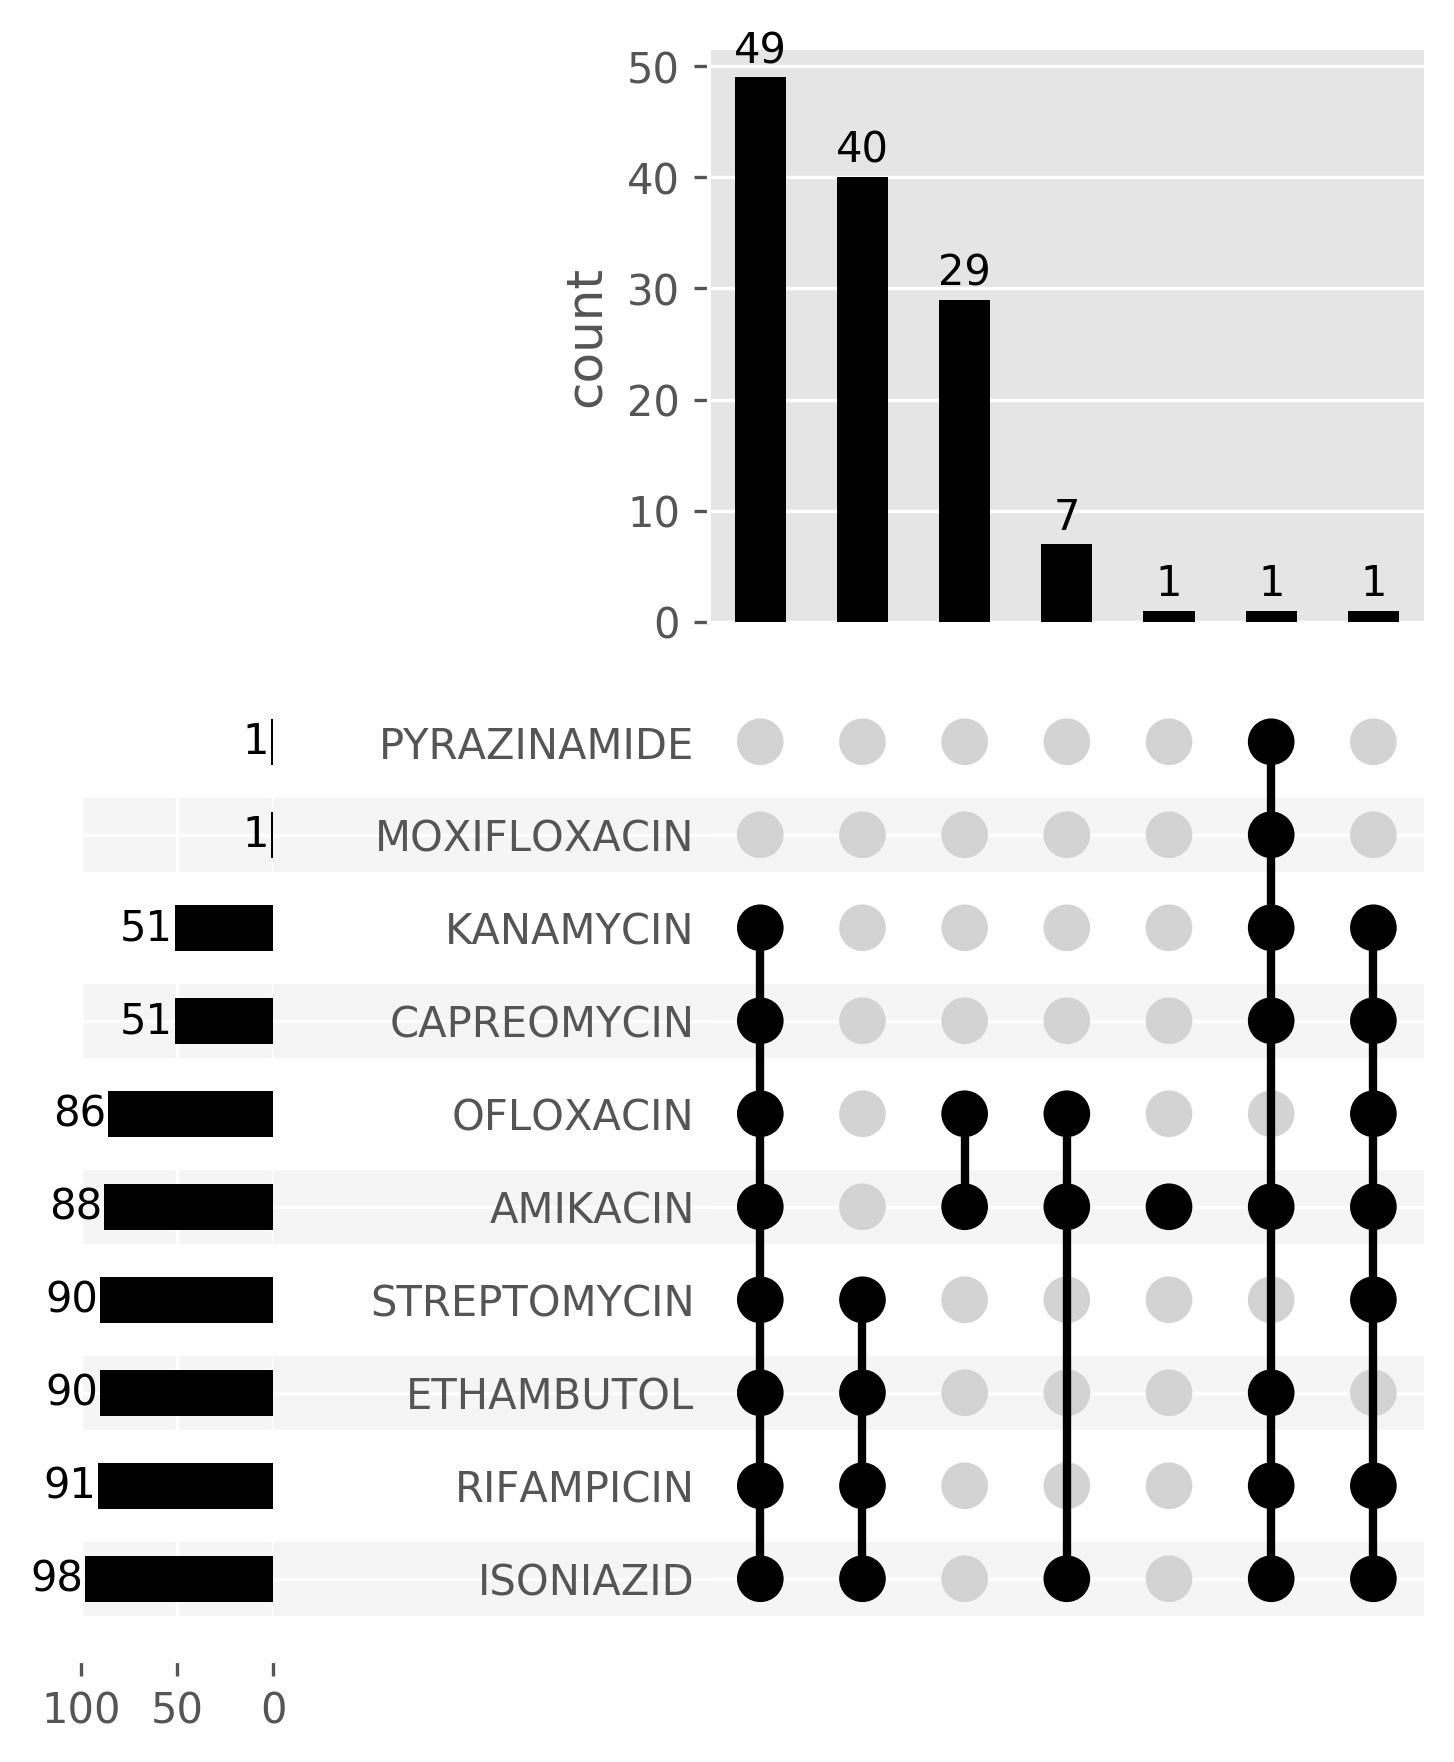
\includegraphics[width=0.90\columnwidth]{Chapter3/Figs/available_dst.png}
\caption{{Culture-based drug susceptibility data available for samples. Each row is a drug, and the columns represent a set of samples with phenotype information for those drugs with a filled cell. The top panel shows the number of samples in the set for that combination of drugs. The bar plot in the left panel shows the number of samples with phenotype information for that drug.
{\label{fig:available-dst}}
}}
\end{center}
\end{figure}
%=========================================================================
\section{Drug resistance prediction with genome graphs}
\label{sec:drprg-methods}

In this section, we describe a method to use genome graphs for predicting drug resistance in \mtb{}; building on previous work in this thesis constructing \mtb{} \panrg{}s (\autoref{sec:tbprg}) and calling variants (\autoref{sec:pandora-filters} and \autoref{chap:denovo}). The tool we developed, \drprg{} (Drug Resistance Prediction with Reference Graphs), is written in the Rust programming language and can be found at \url{https://github.com/mbhall88/drprg}.

While tools already exist to predict \mtb{} AMR, the unique component of \drprg{} is the ability to call novel variants. As the \cryptic{} Consortium recently showed, refusing to predict drug phenotypes in cases where "unknown" mutations are present in the associated target gene can lead to increased detection of pan-susceptibility for first-line drugs \cite{cryptic2018}. However, no tool usable by others was made available in that work, and reproducing the results requires running multiple separate tools and scripts. \drprg{} offers a single program for producing this information.

\drprg{} has two distinct phases. In the first phase, we build an index and (optionally) a \panrg{} from a panel (catalogue) of mutations known to cause resistance or susceptibility. Second, we genotype Illumina or \ont{} reads against the \panrg{}, and phenotype predictions are made for the drugs in the provided panel.

We now outline these two steps in detail.

\subsection{Constructing a panel reference graph}
\label{sec:drprg-index}

The first stage of predicting drug resistance from \drprg{} is coordinated by the \vrb{build} subcommand. As input, \vrb{build} requires a panel of mutations and a reference genome and annotation. We use the reference and annotation for the \mtb{} strain H37Rv (accession NC\_000962.3) and the default panel used by \mykrobe{} (v0.10.0) \cite{hunt2019}.

The panel of variants can be either resistance- or susceptibility-associated. Each entry in the panel file describes the gene the variant occurs in, the mutation it causes, and any drug it impacts. The mutation can represent a nucleic or amino acid change and is of the form reference, position, alternate. For example, a DNA mutation, \vrb{A5T}, indicates the reference base, \vrb{A}, at position 5 in the gene, is changed to a \vrb{T}. An \vrb{X} indicates any nucleic or amino acid other than the one listed as the reference.

After loading the panel, we generate a reference sequence for each listed gene using the provided reference genome and annotation. If the optional padding argument is given, we add the provided number of bases to the start and end of each gene sequence; we use 100bp of padding for the work in this chapter.

The next step is to convert the panel into a VCF representation. For protein mutations, we convert the amino acids into their respective DNA forms (all possible codons). We confirm that the reference codon matches the reference sequence at the given position in the gene. Protein coordinates (positions) are carefully converted to nucleic acid-space, taking into account the transcription strand specified in the annotation. DNA mutations are likewise checked against the reference. A VCF entry is then generated for each panel entry using the DNA representation. For protein mutations and DNA mutations with an alternate allele of \vrb{X}, all possible changes (except stop codons) are listed in the entry. \autoref{fig:example-panel} shows an example panel and associated VCF.

Another optional parameter of \drprg{} \vrb{build} is the ability to provide a prebuilt \panrg{}. If no prebuilt \panrg{} is provided, \drprg{} will construct one from the panel. (The previous steps just outlined remain the same regardless of whether a prebuilt \panrg{} is provided.) \drprg{} builds a panel-based \panrg{} in a similar fashion to the method described in \autoref{sec:tbprg}. That is, for each VCF entry and alternate allele, we replace the gene reference position(s) with the alternate and combine all such mutated sequences into a single FASTA file. We perform a multiple sequence alignment (MSA) on each file, followed by converting the MSA into a local \prg{} using \makeprg{} (\autoref{sec:make_prg}). Finally, the resulting local \prg{}s, which represent each gene in the panel, are combined into a single \panrg{} and indexed with \pandora{}.

For the work in this chapter, we chose to use a prebuilt, population-based \panrg{}, rather than the panel \panrg{} constructed by \drprg{}. We chose a prebuilt \panrg{} because, in the early stages of testing and developing \drprg{}, we found the panel-based \panrg{} density and lack of haplotype information were causing a lot of missed resistance (false negatives). \autoref{app:panel-prg-issues} provides a thorough investigation into these problems with the panel-based \panrg{}.

The population-based \panrg{} we use is built from the same variants as the sparse \panrg{} in \autoref{sec:tbprg} - with an important difference. In \autoref{sec:improve-prg} we discussed a potential improvement for the \panrg{} construction process whereby whole haplotypes are applied to a reference sequence. When we constructed the original sparse \panrg{} in \autoref{sec:tbprg}, we applied each variant, \emph{in isolation}, to the reference sequence. So, if a sample has 3 variants, we built the \prg{} from the reference sequence, plus 3 mutated versions of that reference (see \autoref{sec:improve-prg} for a detailed example). Instead, for the \panrg{} we use in this chapter, we apply \emph{all} variants for a sample in the sparse VCF to the (gene) reference sequence - producing a single (gene) haplotype sequence for that sample. We do this for all genes, and use the same MSA, \makeprg{}, \pandora{} index approach mentioned above (and in \autoref{sec:tbprg}). One major difference being the use of a \makeprg{} prototype (v0.2 - mentioned in \autoref{sec:fw-comp-perf}) with a minimum match length of 5. This prototype, developed by Leandro Ishi, retains information about the clustering of sites for each local \prg{}, allowing for quicker updating of \prg{}s with novel variants (as discussed in \autoref{sec:drprg-predict}).


\subsection{Predicting resistance phenotype}
\label{sec:drprg-predict}

The second and final stage of predicting drug resistance with \drprg{} is the \vrb{predict} routine. It takes an index produced by \drprg{} \vrb{build} (\autoref{sec:drprg-index}) and a file containing sequencing reads (Illumina or \ont{}). One optional parameter of interest for the work in this chapter is the ability to discover novel variants.

If requested, the first stage of \drprg{} \vrb{predict} is novel variant discovery in the sequencing reads with \pandora{} \vrb{discover} (version 0.9.0). This version of \pandora{} differs to the one used in \autoref{chap:clustering} in that it outputs all novel variants into a single file compatible with the \makeprg{} prototype used in \autoref{sec:drprg-index}. Next, \makeprg{} updates the \drprg{} \panrg{} with these new variants and the resulting updated \panrg{} is indexed with \pandora{}. 

One downside to using a population-based \panrg{} as we do, is that unlike the panel-based \panrg{}, it does not contain all panel variants. As such, for the work in this chapter, we request novel variant discovery in \drprg{} \vrb{predict}.

The second step of \vrb{predict} is genotyping of the sample's sequencing data against the \panrg{} (updated or original depending on if variant discovery is requested) with \pandora{} \vrb{map}. An important part of the genotyping step is that we force \pandora{} to output variant coordinates with respect to the gene reference sequences in the index from \vrb{build}. That way, the resulting genotyped VCF coordinates can be compared to the panel VCF constructed in \autoref{sec:drprg-index}. 

After producing the \pandora{} genotyped VCF, we filter out variants that do not meet the provided filtering criteria. \drprg{} \vrb{predict} allows filtering based on: minimum and maximum read depth, strand bias, minimum genotype confidence, minimum fraction of read support (FRS), and maximum indel size. (See \autoref{sec:pandora-filters} for more information on these fields). For the results presented in this chapter, we use a minimum read depth of 3, a minimum FRS of 70\%, a minimum genotype confidence score of 5, a maximum indel size of 20, and a minimum strand bias of 1\% (i.e., we require at least 1\% of total read depth on both strands). We ignore a variant in all subsequent analyses if it fails any of these filters.

Next, we make resistance predictions from the variants that pass filtering. For each call in the genotyped VCF, we fetch all entries in the panel VCF that have overlapping coordinates. If there are no panel variants that overlap the call and novel variant discovery is requested, we classify all drugs associated with the gene of the present call as "unknown" (`U'). If the call is a null genotype (\vrb{.}), we predict all overlapping panel variants as "failed" (`F').

If the variant call was not deemed unknown or failed in the previous step, we check for a match between the call and a panel allele. To determine whether a match exists, we iterate through each panel allele (including the reference) and extract an overlapping sequence between it and the called sequence. If the panel and called allele start at the same position, this is as simple as trimming both sequences to the shortest length of the two. Otherwise, we extract the subsequence denoted by the intersection between the two allele's intervals if they start at different positions. 

For example, if the called allele, \vrb{AT}, starts at position 4 and the panel allele, \vrb{TG}, starts at position 5, their (half-open) intervals are $[4,6)$ and $[5,7)$ respectively. Thus, the intersection of these two alleles would be $[5,6)$, which yields a matching subsequence of \vrb{T} for both. When the two alleles do not have the same length - e.g., indels - we also track the matching sequences' length relative to the reference allele. That way, when there is more than one panel allele that matches the called allele, we return the allele with the match whose length is closest to the called allele.

We add two annotations to each of the genotyped VCF entries that overlap variants in the panel: \vrb{VARID} and \vrb{PREDICT}. \vrb{VARID} is a list of panel variants the position overlaps, and \vrb{PREDICT} is a prediction for each of those panel variants. If there was a non-reference match between a panel variant and the called allele, and the panel variant is resistance-causing, a resistant prediction is recorded. If there was no match, or the match is with the reference allele, the prediction is susceptible; unless variant discovery was requested, in which case the prediction is unknown. 

After adding the prediction annotations to each entry in the genotyped VCF, we produce a final prediction report as a JSON file. A prediction is provided for every drug present in the panel, along with the supporting evidence (variant(s)). We generate these predictions by going back through the genotyped VCF and using the \vrb{PREDICT} annotation added in the previous step. When different predictions are present for the same drug, the precedence, in order, is resistant, unknown, failed, and susceptible. \autoref{fig:example-drprg-report} shows an example report.

\noindent
All \drprg{} results in this chapter were generated using the commit \href{https://github.com/mbhall88/drprg/tree/cb4f9b82b5d03de45b8016ae5d54bbce7a8f3a0f}{\vrb{cb4f9b8}}.

\subsection{Computational performance}
\label{sec:drprg-comp-perf}

We compare the peak memory usage and runtime for \drprg{} \vrb{predict} with \mykrobe{} - another genome graph-based AMR predictor. \autoref{fig:predict-comp-perf} shows the computational performance of both tools, split by sequencing technology. On average, \drprg{} is faster than \mykrobe{} for both Illumina and \ont{} and uses less memory. As summarised in \autoref{tab:predict-comp-pref}, \drprg{} has a median CPU time of 111.84s (Illumina) and 178.41s (\ont{}) compared to \mykrobe{}'s 196.90s (Illumina) and 248.81s (\ont{}). For memory usage, \drprg{} had a median peak of 224MB (Illumina) and 345.50MB (\ont{}) compared with \mykrobe{}'s 1193MB (Illumina) and 1195MB (\ont{}). However, these time and memory statistics are more than sufficient for both tools to be comfortably run on a standard laptop. 

Building the \drprg{} population-based \panrg{} and index took 174.53s of CPU time and had a peak memory usage of 368MB, which occurred during the \makeprg{} step.

\begin{figure}
\begin{center}
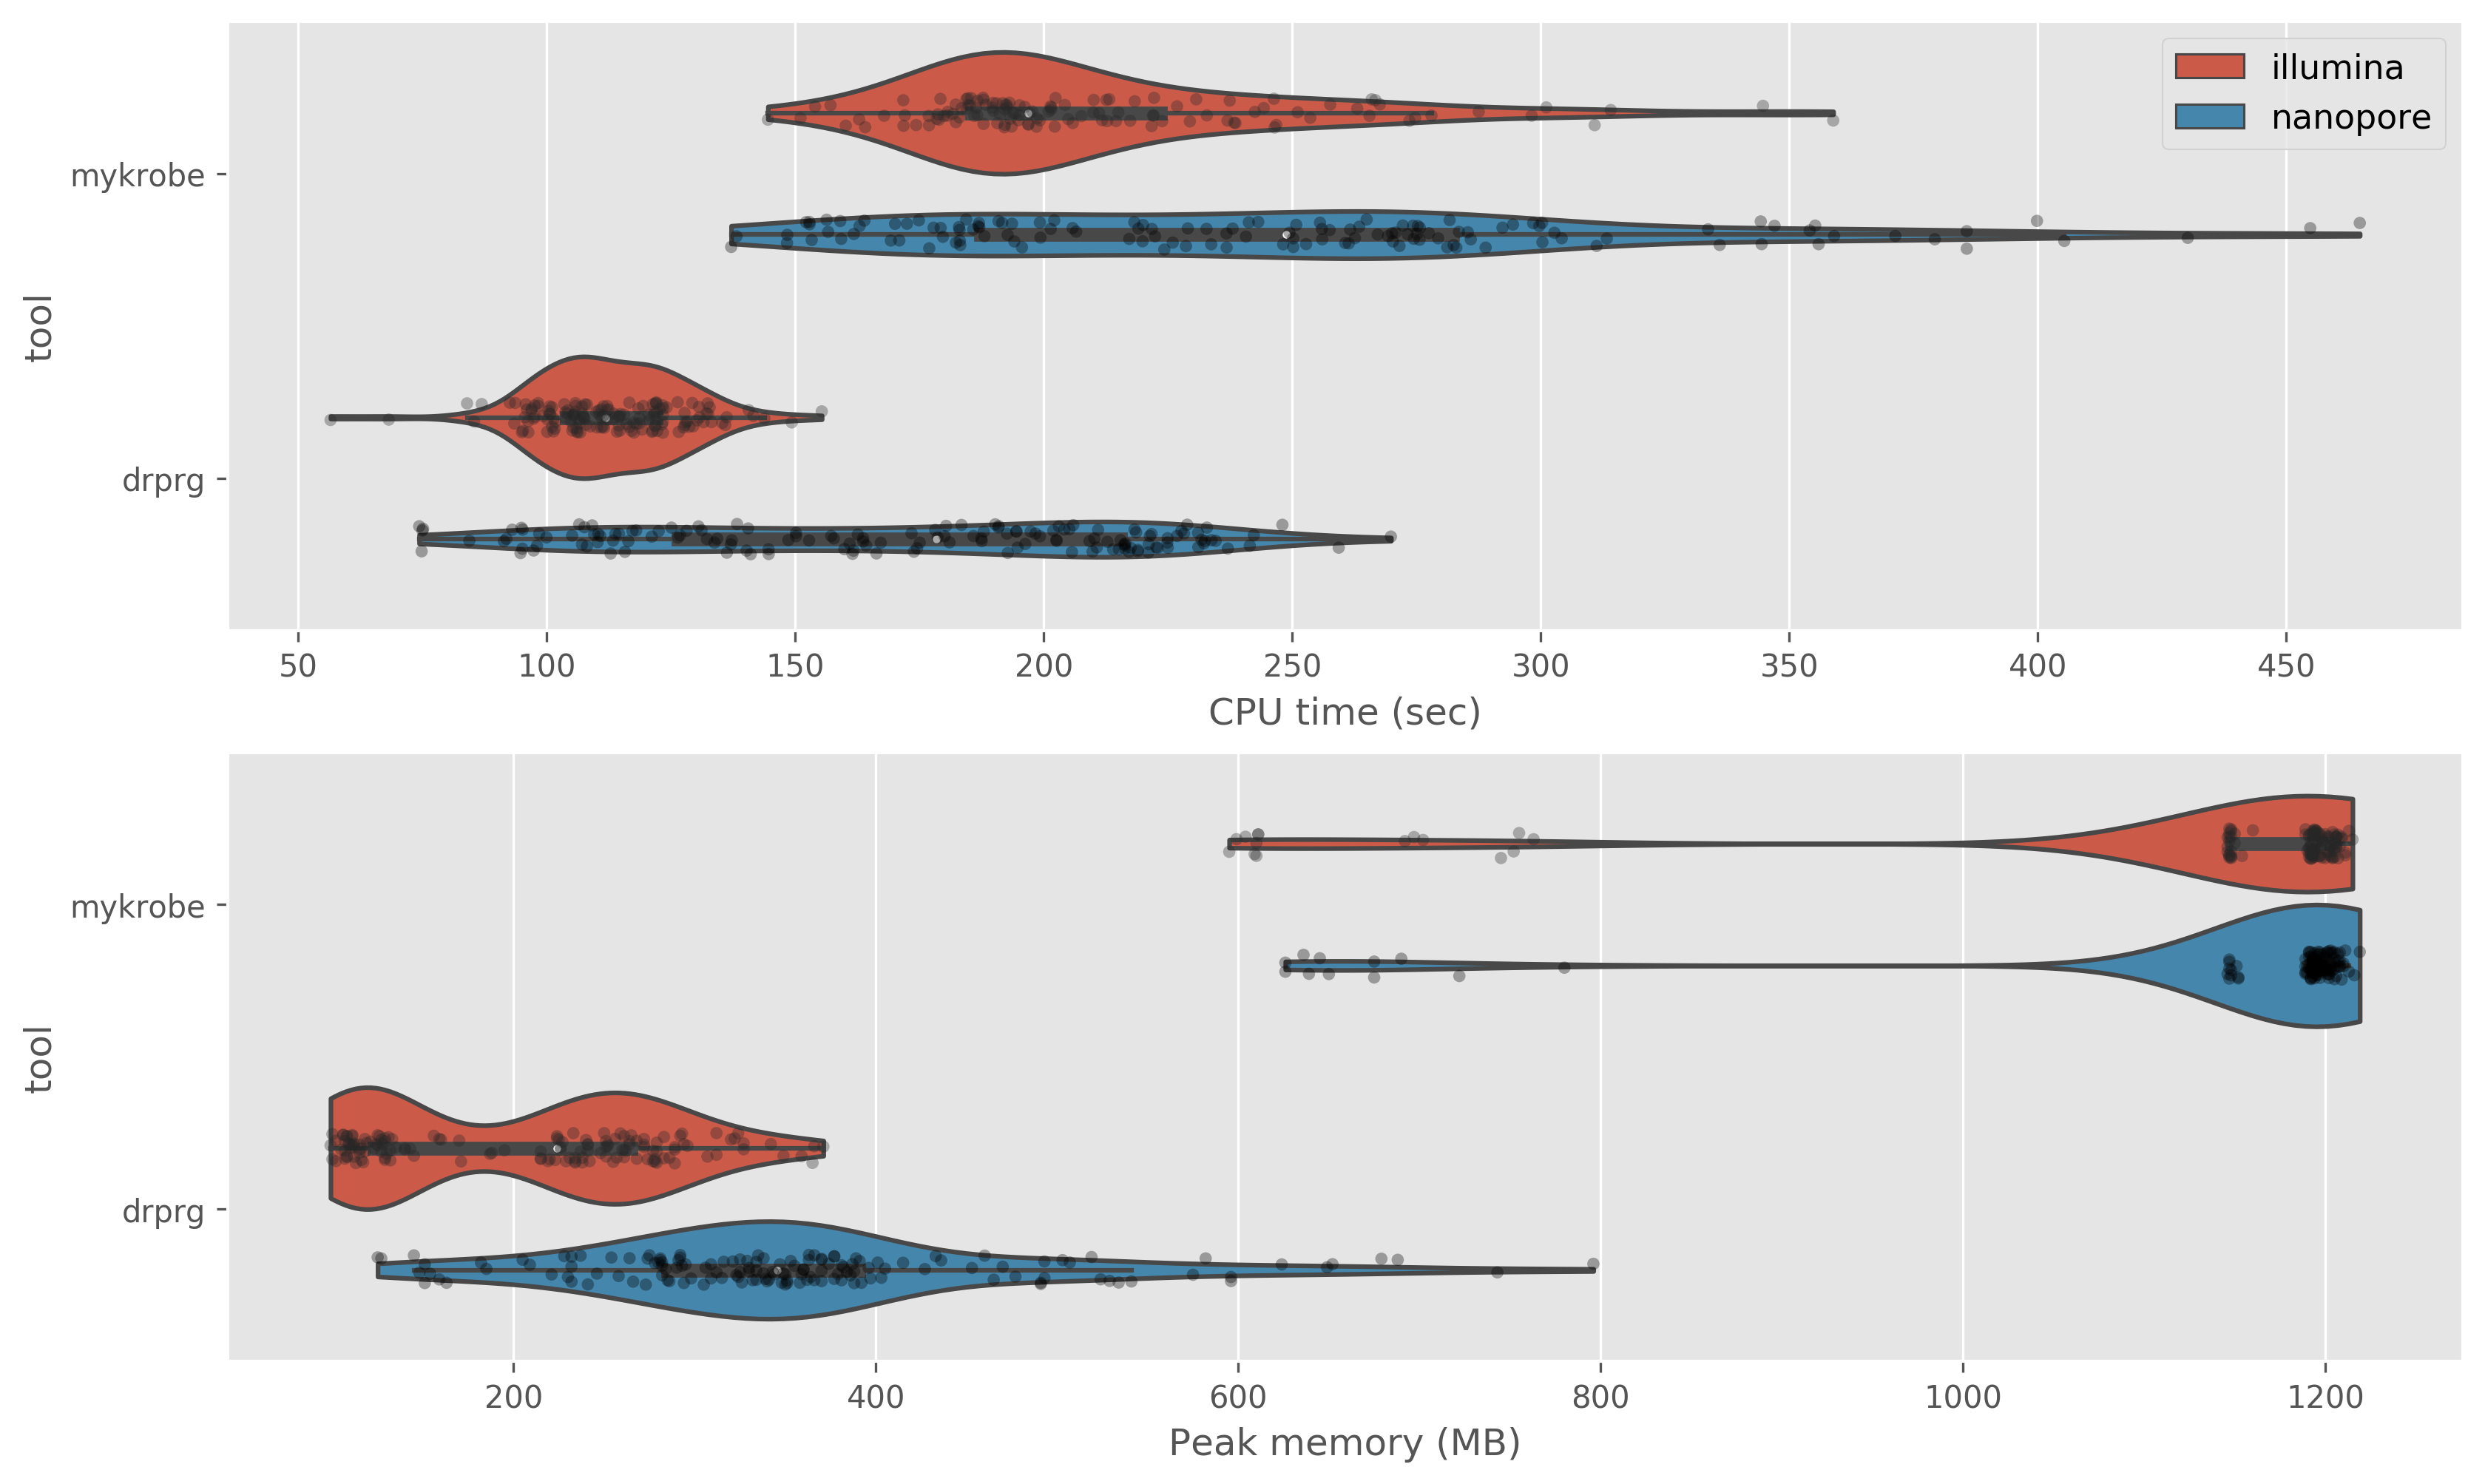
\includegraphics[width=0.90\columnwidth]{Chapter3/Figs/predict-comp-perf.png}
\caption{{The time (seconds; top) and memory (megabytes; bottom) usage of \mykrobe{} and \drprg{} for generating drug resistance predictions. Each tool is additionally split into sequencing technology, with Illumina in red and \ont{} in blue. Data points indicate individual results for a single sample.
{\label{fig:predict-comp-perf}}
}}
\end{center}
\end{figure}


\begin{table}
\centering
\resizebox{\textwidth}{!}{%
\begin{tabular}{@{}llllll@{}}
\toprule
\multicolumn{2}{l}{Tool}       & \multicolumn{2}{l}{\drprg{}} & \multicolumn{2}{l}{\mykrobe{}} \\ \midrule
\multicolumn{2}{l}{Technology} & Illumina       & \ont{}      & Illumina        & \ont{}       \\
\multirow{7}{*}{time (s)}    & mean & 112.85 & 170.06 & 209.71  & 247.75  \\
                             & std  & 14.37  & 49.28  & 38.59   & 69.85   \\
                             & min  & 56.51  & 74.34  & 144.51  & 137.11  \\
                             & 25\% & 103.95 & 126.50 & 185.55  & 187.29  \\
                             & 50\% & \textbf{111.84} & \textbf{178.41} & 196.90  & 248.81  \\
                             & 75\% & 122.05 & 215.37 & 223.41  & 282.25  \\
                             & max  & 155.34 & 269.84 & 358.83  & 464.77  \\
\midrule
\multirow{7}{*}{memory (MB)} & mean & 203.28 & 357.47 & 1126.33 & 1151.14 \\
                             & std  & 78.64  & 121.38 & 173.29  & 145.87  \\
                             & min  & 99.00  & 125.00 & 595.00  & 626.00  \\
                             & 25\% & 123.25 & 285.25 & 1148.50 & 1192.00 \\
                             & 50\% & \textbf{224.00} & \textbf{345.50} & 1193.00 & 1195.00 \\
                             & 75\% & 264.75 & 390.50 & 1201.00 & 1201.00 \\
                             & max  & 371.00 & 796.00 & 1215.00 & 1219.00 \\ \cmidrule(l){2-6} 
\end{tabular}%
}
\caption{Summary statistics for the CPU time and peak memory usage of drug resistance prediction with \mykrobe{} and \drprg{} for Illumina and \ont{} data. std=standard deviation}
\label{tab:predict-comp-pref}
\end{table}

%=========================================================================
\section{Concordance of \ont{}-based resistance predictions with Illumina}
\label{sec:geno-concordance}

The first step in assessing \ont{}-based AMR predictions is to compare its level of agreement with genotype-based predictions from Illumina data, which have been extensively validated elsewhere (\autoref{sec:amr}).

We compare the WGS-based drug resistance predictions from \mykrobe{} (version 0.10.0; \cite{hunt2019}) and \drprg{} for both Illumina and \ont{} data, using the same catalogue of resistance-causing mutations. For the predictions from \mykrobe{}, we altered some default settings as a result of the analysis in \autoref{app:mykrobe-settings}. The Illumina expected error rate was decreased from 0.05 (default) to 0.001, and the preset \ont{} settings were disabled in favour of an expected error rate of 0.08 and disabling minor resistance calls (haploid model). The \drprg{} settings are detailed in \autoref{sec:drprg-predict}. 

For this genotype concordance analysis, we assume the Illumina predictions from \mykrobe{} are the true phenotype and compare the \mykrobe{} \ont{} and \drprg{} (both modalities) predictions accordingly. For each drug/sample combination, we classify the WGS predictions as true-positive (TP) or -negative (TN) when the prediction is resistant or susceptible, respectively, and matches the \mykrobe{}-Illumina prediction. When the predictions do not match \mykrobe{}-Illumina, we classify them as false-positive (FP) or -negative (FN) for resistance or susceptible predictions, respectively. For this concordance analysis, we ignore failed, and unknown resistance calls from \drprg{} and consider them as susceptible (we assess the utility of these features in \autoref{sec:drprg-discover}). Additionally, for \mykrobe{} Illumina predictions, we interpret minor resistance calls (`r') as resistance (`R').

Given the comprehensive validation of \mykrobe{}'s prediction power on Illumina data \cite{hunt2019,bradley2015}, if \ont{} results are concordant, this will go a long way to endorsing its use for AMR prediction. In addition, if the Illumina and \ont{} predictions from \drprg{} are consistent with \mykrobe{}, this is an excellent first validation of the method.

Across all drugs, there was 8 FN (missed resistance) calls by \mykrobe{} \ont{}. Seven of those FNs are situations where the Illumina data has called minor resistance - a heterozygous call at a resistance-causing variant. As we use a haploid model for \ont{} (see \autoref{app:mykrobe-settings}), this is unavoidable until a model that allows complex ploidy can be employed. We did attempt to use a diploid model for \ont{}, but found a dramatic increase in the number of FNs and FPs due to indel calls.

For the \drprg{} \ont{} predictions, there were 32 FNs across all drugs. Ten of these were cases where \mykrobe{} called minor resistance. Similar to \mykrobe{} for \ont{}, \drprg{} employs a haploid model for both Illumina and \ont{}; therefore, heterozygous calls are not possible. Another 14 FNs were called resistance by \drprg{} \ont{}, but the variant was filtered due to low FRS - meaning we call susceptible. All but one of these FRS cases was a promoter mutation C-15X in \textit{fabG1}. A further two FNs were also filtered out due to strand bias. Lastly, five FNs were associated with indel calls in \textit{pncA}; indels are a known systematic problem with \ont{} data \cite{watson2019}.

\drprg{} with Illumina data missed 17 resistance calls compared to \mykrobe{} with Illumina. Ten of these were cases of \mykrobe{} calling minor resistance, as mentioned above. Of the remaining 7 FNs, four were related to indel calls in \textit{pncA}, and three have no evidence in the \drprg{} VCF.

Of the 17 FPs made by \mykrobe{} \ont{}, nine show strong support for the resistance-causing variant in the VCFs from \autoref{sec:var-calls} for both technologies. In each of these cases, the \mykrobe{} results from Illumina also called the variant but filtered it out due to low coverage. A further eight are false-positive isoniazid indel calls made by \ont{} in a GC-rich region of \textit{katG}.

The \drprg{} predictions had 23 and 22 FPs for \ont{} and Illumina data respectively. The one difference being the \ont{} predictions have one more isoniazid FP from a \textit{katG} indel call. 11/23 FPs are associated with indel calls in \textit{pncA} causing a false resistance call for pyrazinamide. Indel calls were also the cause of two FPs for isoniazid (\textit{katG}) and one for rifampicin (\textit{rpoB}). Similar to the \mykrobe{} \ont{} calls, 10 of the \drprg{} FPs showed strong support for the resistance-causing variant in VCFs (\autoref{sec:var-calls}) for both technologies, with the \mykrobe{} results from Illumina having also called the variant, but filtered out due to low coverage. Additionally, in 11 FPs, the culture-based phenotype supports the \drprg{} prediction.


\begin{figure}
\begin{center}
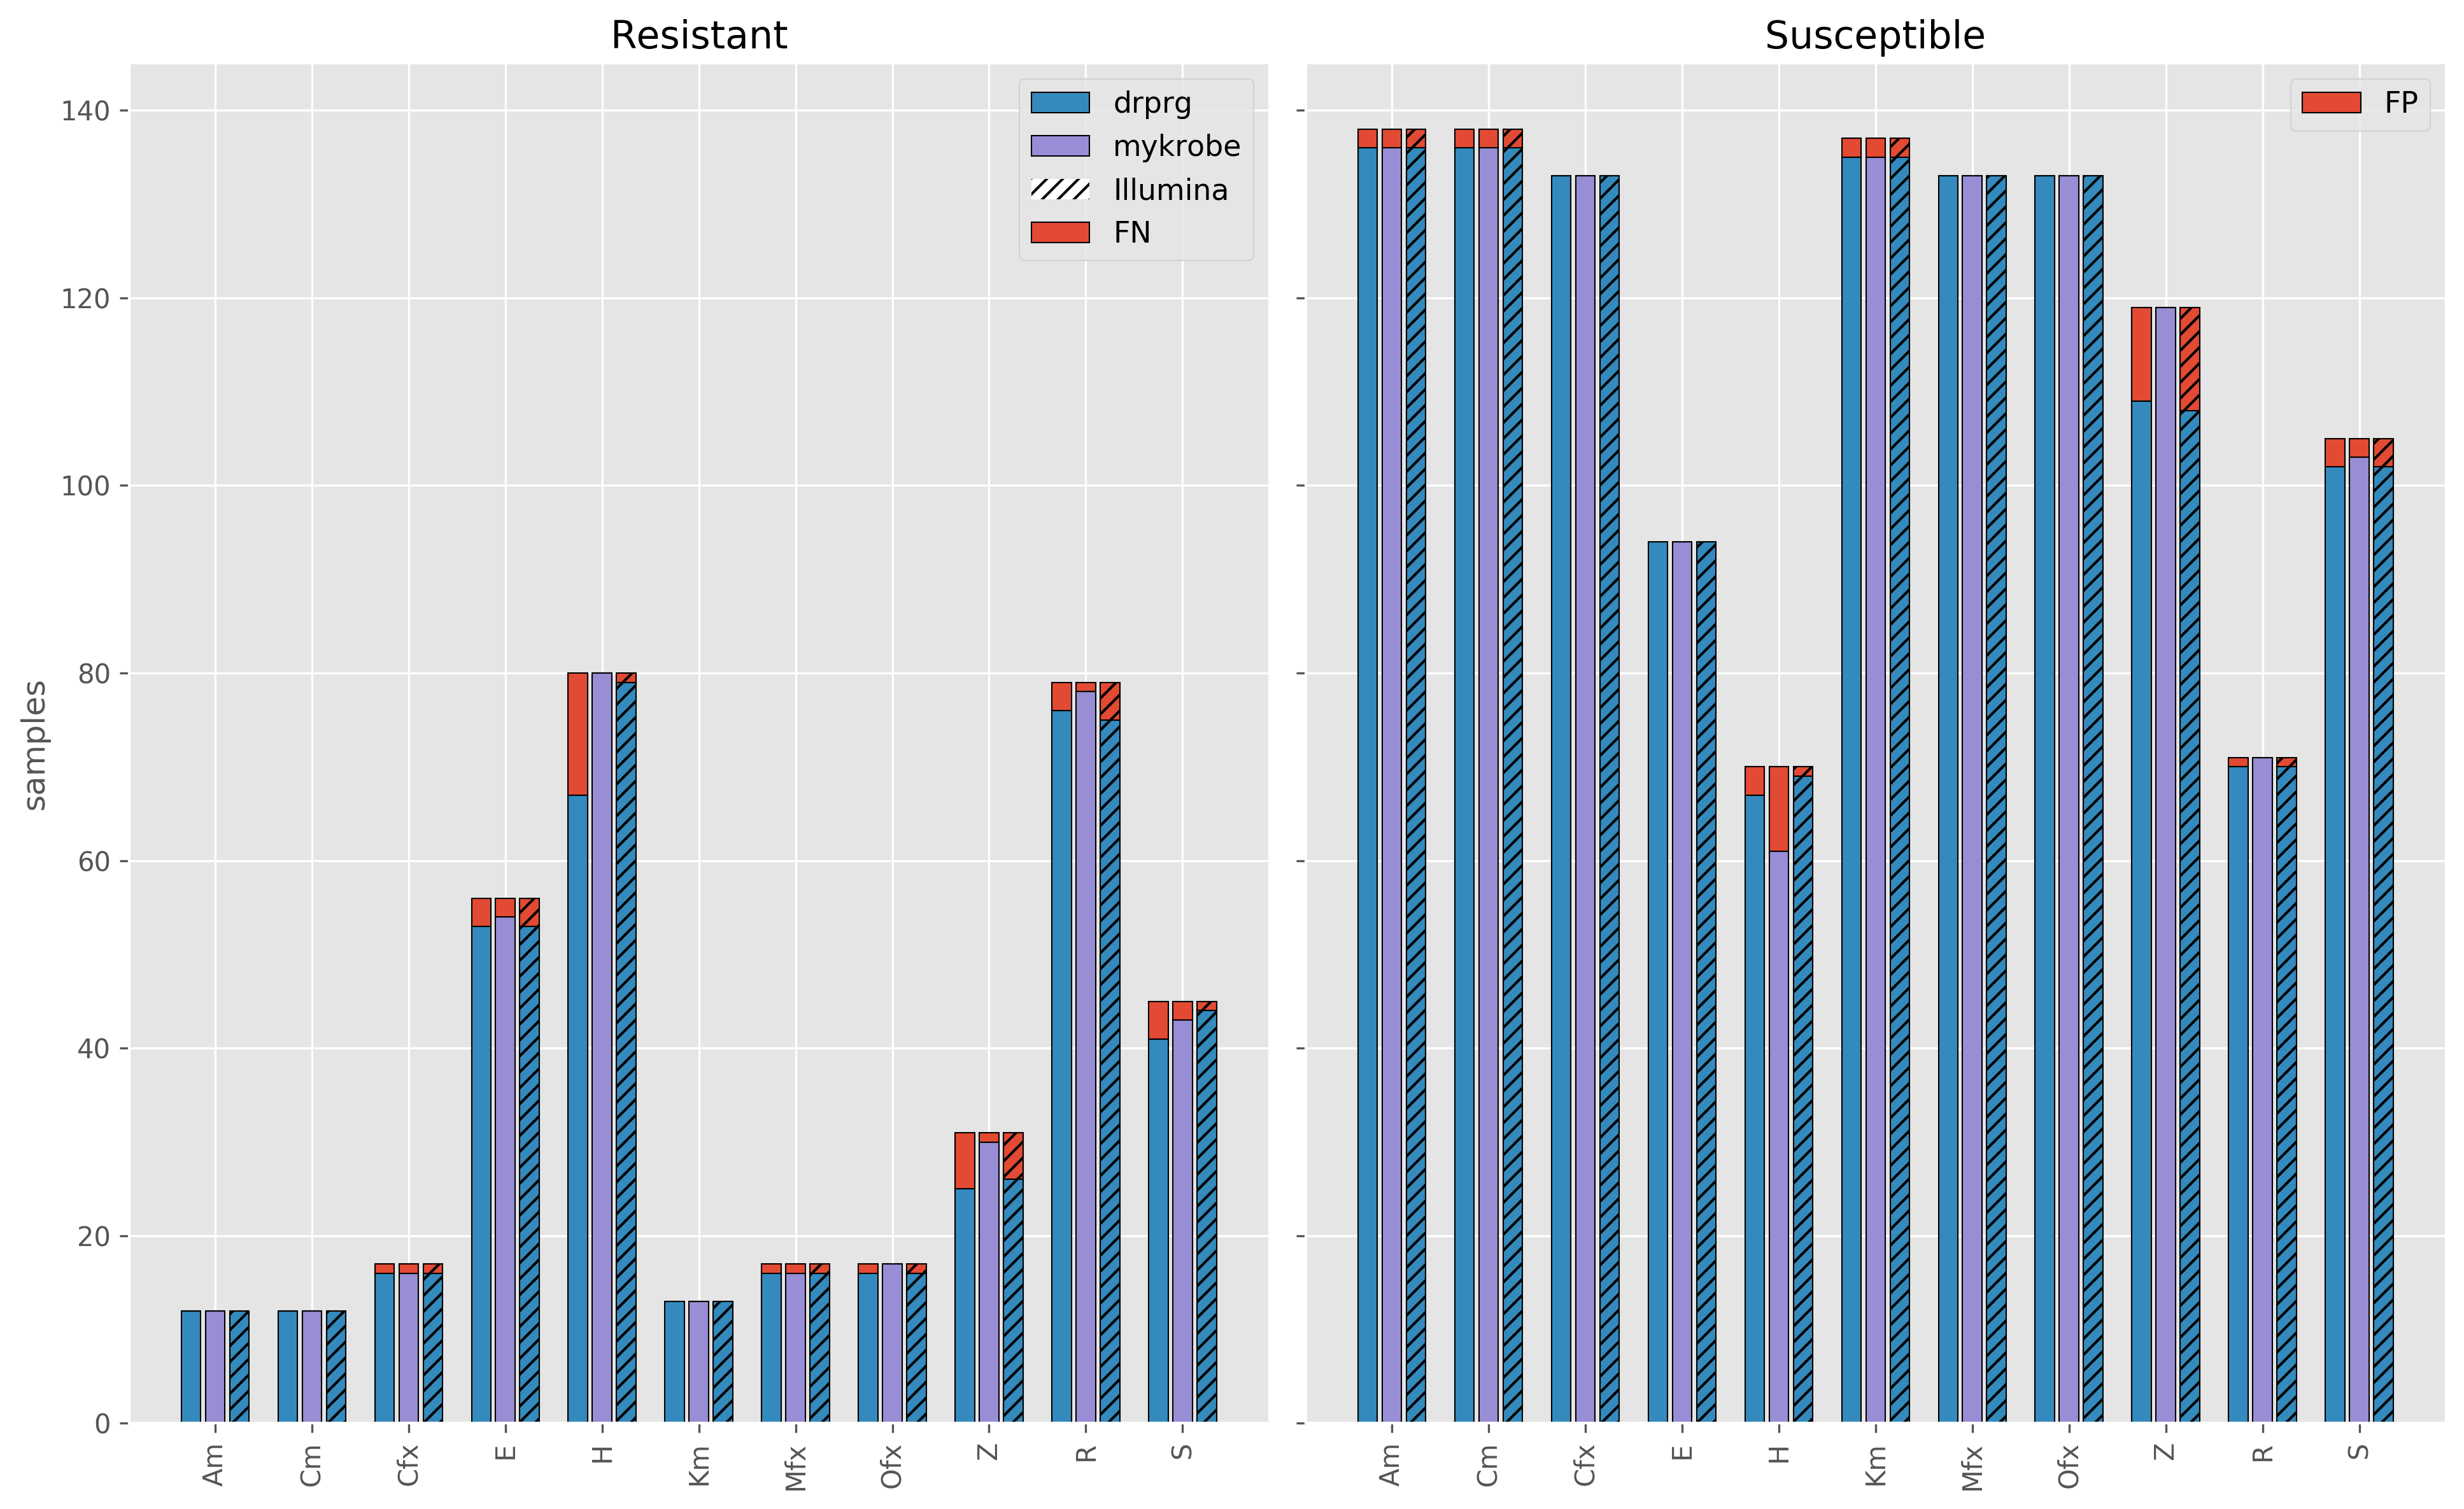
\includegraphics[width=0.90\columnwidth]{Chapter3/Figs/illumina_concordance.png}
\caption{{Number of resistant (left) and susceptible (right) WGS-based drug resistance phenotypes correctly predicted by \mykrobe{} \ont{} (purple) and \drprg{} (blue) with Illumina (striped) and \ont{} (non-striped) data. For this analysis, the Illumina-based \mykrobe{} predictions are considered truth and the other predictions are assessed accordingly. The red bars indicate missed (FN) or incorrect (FP) predictions. The x-axis shows the drugs for which \mykrobe{} makes predictions. E - ethambutol; H - isoniazid; Z - pyrazinamide; R - rifampicin; S - streptomycin; Km - kanamycin; Am - amikacin; Ofx - ofloxacin; Cm - capreomycin; Mfx - moxifloxacin.
{\label{fig:geno-concordance}}
}}
\end{center}
\end{figure}

\begin{table}
\centering
\resizebox{\textwidth}{!}{%
\begin{tabular}{@{}lllllllll@{}}
\toprule
Drug &
  Tool &
  Technology &
  FN(R) &
  FP(S) &
  FNR(95\% CI) &
  FPR(95\% CI) &
  PPV(95\% CI) &
  NPV(95\% CI) \\ \midrule
\multirow{3}{*}{Amikacin} &
  \multirow{2}{*}{\drprg{}} &
  Illumina &
  0(12) &
  2(138) &
  0.0\% (0.0-24.2\%) &
  1.4\% (0.4-5.1\%) &
  85.7\% (60.1-96.0\%) &
  100.0\% (97.3-100.0\%) \\
 &
   &
  \multirow{2}{*}{Nanopore} &
  0(12) &
  2(138) &
  0.0\% (0.0-24.2\%) &
  1.4\% (0.4-5.1\%) &
  85.7\% (60.1-96.0\%) &
  100.0\% (97.3-100.0\%) \\
 &
  \mykrobe{} &
   &
  0(12) &
  2(138) &
  0.0\% (0.0-24.2\%) &
  1.4\% (0.4-5.1\%) &
  85.7\% (60.1-96.0\%) &
  100.0\% (97.3-100.0\%) \\ \cmidrule(l){2-9} 
\multirow{3}{*}{Capreomycin} &
  \multirow{2}{*}{\drprg{}} &
  Illumina &
  0(12) &
  2(138) &
  0.0\% (0.0-24.2\%) &
  1.4\% (0.4-5.1\%) &
  85.7\% (60.1-96.0\%) &
  100.0\% (97.3-100.0\%) \\
 &
   &
  \multirow{2}{*}{Nanopore} &
  0(12) &
  2(138) &
  0.0\% (0.0-24.2\%) &
  1.4\% (0.4-5.1\%) &
  85.7\% (60.1-96.0\%) &
  100.0\% (97.3-100.0\%) \\
 &
  \mykrobe{} &
   &
  0(12) &
  2(138) &
  0.0\% (0.0-24.2\%) &
  1.4\% (0.4-5.1\%) &
  85.7\% (60.1-96.0\%) &
  100.0\% (97.3-100.0\%) \\ \cmidrule(l){2-9} 
\multirow{3}{*}{Ciprofloxacin} &
  \multirow{2}{*}{\drprg{}} &
  Illumina &
  1(17) &
  0(133) &
  5.9\% (1.0-27.0\%) &
  0.0\% (0.0-2.8\%) &
  100.0\% (80.6-100.0\%) &
  99.3\% (95.9-99.9\%) \\
 &
   &
  \multirow{2}{*}{Nanopore} &
  1(17) &
  0(133) &
  5.9\% (1.0-27.0\%) &
  0.0\% (0.0-2.8\%) &
  100.0\% (80.6-100.0\%) &
  99.3\% (95.9-99.9\%) \\
 &
  \mykrobe{} &
   &
  1(17) &
  0(133) &
  5.9\% (1.0-27.0\%) &
  0.0\% (0.0-2.8\%) &
  100.0\% (80.6-100.0\%) &
  99.3\% (95.9-99.9\%) \\ \cmidrule(l){2-9} 
\multirow{3}{*}{Ethambutol} &
  \multirow{2}{*}{\drprg{}} &
  Illumina &
  3(56) &
  0(94) &
  5.4\% (1.8-14.6\%) &
  0.0\% (0.0-3.9\%) &
  100.0\% (93.2-100.0\%) &
  96.9\% (91.3-98.9\%) \\
 &
   &
  \multirow{2}{*}{Nanopore} &
  3(56) &
  0(94) &
  5.4\% (1.8-14.6\%) &
  0.0\% (0.0-3.9\%) &
  100.0\% (93.2-100.0\%) &
  96.9\% (91.3-98.9\%) \\
 &
  \mykrobe{} &
   &
  2(56) &
  0(94) &
  3.6\% (1.0-12.1\%) &
  0.0\% (0.0-3.9\%) &
  100.0\% (93.4-100.0\%) &
  97.9\% (92.7-99.4\%) \\ \cmidrule(l){2-9} 
\multirow{3}{*}{Isoniazid} &
  \multirow{2}{*}{\drprg{}} &
  Illumina &
  1(80) &
  1(70) &
  1.2\% (0.2-6.7\%) &
  1.4\% (0.3-7.7\%) &
  98.8\% (93.3-99.8\%) &
  98.6\% (92.3-99.7\%) \\
 &
   &
  \multirow{2}{*}{Nanopore} &
  13(80) &
  3(70) &
  \textbf{16.2\% (9.7-25.8\%)} &
  4.3\% (1.5-11.9\%) &
  95.7\% (88.1-98.5\%) &
  83.8\% (74.2-90.3\%) \\
 &
  \mykrobe{} &
   &
  0(80) &
  9(70) &
  0.0\% (0.0-4.6\%) &
  \textbf{12.9\% (6.9-22.7\%)} &
  89.9\% (81.9-94.6\%) &
  100.0\% (94.1-100.0\%) \\ \cmidrule(l){2-9} 
\multirow{3}{*}{Kanamycin} &
  \multirow{2}{*}{\drprg{}} &
  Illumina &
  0(13) &
  2(137) &
  0.0\% (0.0-22.8\%) &
  1.5\% (0.4-5.2\%) &
  86.7\% (62.1-96.3\%) &
  100.0\% (97.2-100.0\%) \\
 &
   &
  \multirow{2}{*}{Nanopore} &
  0(13) &
  2(137) &
  0.0\% (0.0-22.8\%) &
  1.5\% (0.4-5.2\%) &
  86.7\% (62.1-96.3\%) &
  100.0\% (97.2-100.0\%) \\
 &
  \mykrobe{} &
   &
  0(13) &
  2(137) &
  0.0\% (0.0-22.8\%) &
  1.5\% (0.4-5.2\%) &
  86.7\% (62.1-96.3\%) &
  100.0\% (97.2-100.0\%) \\ \cmidrule(l){2-9} 
\multirow{3}{*}{Moxifloxacin} &
  \multirow{2}{*}{\drprg{}} &
  Illumina &
  1(17) &
  0(133) &
  5.9\% (1.0-27.0\%) &
  0.0\% (0.0-2.8\%) &
  100.0\% (80.6-100.0\%) &
  99.3\% (95.9-99.9\%) \\
 &
   &
  \multirow{2}{*}{Nanopore} &
  1(17) &
  0(133) &
  5.9\% (1.0-27.0\%) &
  0.0\% (0.0-2.8\%) &
  100.0\% (80.6-100.0\%) &
  99.3\% (95.9-99.9\%) \\
 &
  \mykrobe{} &
   &
  1(17) &
  0(133) &
  5.9\% (1.0-27.0\%) &
  0.0\% (0.0-2.8\%) &
  100.0\% (80.6-100.0\%) &
  99.3\% (95.9-99.9\%) \\ \cmidrule(l){2-9} 
\multirow{3}{*}{Ofloxacin} &
  \multirow{2}{*}{\drprg{}} &
  Illumina &
  1(17) &
  0(133) &
  5.9\% (1.0-27.0\%) &
  0.0\% (0.0-2.8\%) &
  100.0\% (80.6-100.0\%) &
  99.3\% (95.9-99.9\%) \\
 &
   &
  \multirow{2}{*}{Nanopore} &
  1(17) &
  0(133) &
  5.9\% (1.0-27.0\%) &
  0.0\% (0.0-2.8\%) &
  100.0\% (80.6-100.0\%) &
  99.3\% (95.9-99.9\%) \\
 &
  \mykrobe{} &
   &
  0(17) &
  0(133) &
  0.0\% (0.0-18.4\%) &
  0.0\% (0.0-2.8\%) &
  100.0\% (81.6-100.0\%) &
  100.0\% (97.2-100.0\%) \\ \cmidrule(l){2-9} 
\multirow{3}{*}{Pyrazinamide} &
  \multirow{2}{*}{\drprg{}} &
  Illumina &
  5(31) &
  11(119) &
  \textbf{16.1\% (7.1-32.6\%)} &
  \textbf{9.2\% (5.2-15.8\%)} &
  70.3\% (54.2-82.5\%) &
  95.6\% (90.1-98.1\%) \\
 &
   &
  \multirow{2}{*}{Nanopore} &
  6(31) &
  10(119) &
  \textbf{19.4\% (9.2-36.3\%)} &
  \textbf{8.4\% (4.6-14.8\%)} &
  71.4\% (54.9-83.7\%) &
  94.8\% (89.1-97.6\%) \\
 &
  \mykrobe{} &
   &
  1(31) &
  0(119) &
  3.2\% (0.6-16.2\%) &
  0.0\% (0.0-3.1\%) &
  100.0\% (88.6-100.0\%) &
  99.2\% (95.4-99.9\%) \\ \cmidrule(l){2-9} 
\multirow{3}{*}{Rifampicin} &
  \multirow{2}{*}{\drprg{}} &
  Illumina &
  4(79) &
  1(71) &
  5.1\% (2.0-12.3\%) &
  1.4\% (0.2-7.6\%) &
  98.7\% (92.9-99.8\%) &
  94.6\% (86.9-97.9\%) \\
 &
   &
  \multirow{2}{*}{Nanopore} &
  3(79) &
  1(71) &
  3.8\% (1.3-10.6\%) &
  1.4\% (0.2-7.6\%) &
  98.7\% (93.0-99.8\%) &
  95.9\% (88.6-98.6\%) \\
 &
  \mykrobe{} &
   &
  1(79) &
  0(71) &
  1.3\% (0.2-6.8\%) &
  0.0\% (0.0-5.1\%) &
  100.0\% (95.3-100.0\%) &
  98.6\% (92.5-99.8\%) \\ \cmidrule(l){2-9} 
\multirow{3}{*}{Streptomycin} &
  \multirow{2}{*}{\drprg{}} &
  Illumina &
  1(45) &
  3(105) &
  2.2\% (0.4-11.6\%) &
  2.9\% (1.0-8.1\%) &
  93.6\% (82.8-97.8\%) &
  99.0\% (94.7-99.8\%) \\
 &
   &
  \multirow{2}{*}{Nanopore} &
  4(45) &
  3(105) &
  \textbf{8.9\% (3.5-20.7\%)} &
  2.9\% (1.0-8.1\%) &
  93.2\% (81.8-97.7\%) &
  96.2\% (90.7-98.5\%) \\
 &
  \mykrobe{} &
   &
  2(45) &
  2(105) &
  4.4\% (1.2-14.8\%) &
  1.9\% (0.5-6.7\%) &
  95.6\% (85.2-98.8\%) &
  98.1\% (93.3-99.5\%) \\ \cmidrule(l){2-9} 
\end{tabular}%
}
\caption{Comparison of \drprg{} and \mykrobe{} \ont{} drug resistance predictions with \mykrobe{} Illumina predictions. For this comparison, we assume the \mykrobe{} resistance prediction from Illumina data is correct and evaluate the other predictions accordingly. Bold text is used to highlight differences of note. FN=false negative; R=number of resistant samples; FP=false positive; S=number of susceptible samples; FNR=false negative rate; FPR=false positive rate; PPV=positive predictive value; NPV=negative predictive value; CI=Wilson score confidence interval}
\label{tab:geno-concordance}
\end{table}

\subsection{Summary}

In summary, \mykrobe{} \ont{} AMR predictions are consistent with those from Illumina data. There were some discrepancies; however, all but one of the missed resistance calls was due to heterozygous calls, which \ont{} cannot replicate yet. Additionally, many of the false resistance calls were either \ont{} making incorrect indel calls, or Illumina missing variants with strong support from the analysis in \autoref{sec:var-calls}.

For most drugs, \drprg{} predictions are concordant with \mykrobe{}'s Illumina calls. More than half of the \drprg{} missed resistance calls were due to it not being able to detect heterozygous positions. \drprg{} \ont{} predictions also missed some resistant calls because of a low fraction of read support for the mutation in question. A major reason for false resistance calls from \drprg{}, for both technologies, was incorrect indel calls in \textit{pncA}. However, nearly half of the \drprg{} false positives (SNPs) are potentially missed resistance on \mykrobe{}'s part due to it having filtered out the calls due to low support. 

%=========================================================================
\section{Concordance of genotype-based predictions with culture-based phenotypes}
\label{sec:pheno-concordance}

In this section, we assess the concordance of \ont{} and Illumina WGS genotype-based AMR predictions with gold-standard culture-based DST phenotypes.

We saw in \autoref{sec:geno-concordance} that \ont{}-derived resistance predictions are in line with those from Illumina when comparing to \mykrobe{} Illumina-based predictions. However, as this concordance was not perfect, we explore the agreement of WGS predictions with culture-based phenotype - where this information is available. As we use the same catalogue for all WGS predictions, this analysis aims to assess both the prediction methods and sequencing modalities and determine whether either or both of these factors drive the genotype discrepancies.

The culture-based DST profiles gathered in \autoref{sec:dst-methods} are considered the true phenotype against which we will appraise the WGS methods. We exclude moxifloxacin and pyrazinamide from this analysis as DST is only available for one sample. \autoref{tab:available-dst} outlines the total number of samples with phenotype information for each drug.

We follow the same classification approach as in \autoref{sec:geno-concordance}, but use the culture-based phenotype as the truth and compare the \mykrobe{} and \drprg{} predictions accordingly - for both sequencing technologies.

\autoref{fig:pheno-concordance} shows the concordance of WGS predictions with culture-based phenotypes. The left panel illustrates the number of correct and missed resistance calls made by \mykrobe{} and \drprg{} for both Illumina and \ont{} data. In the right panel, we show the number of correct and incorrect susceptibility predictions. \autoref{tab:pheno-concordance} provides the number of FNs and FPs, along with the false-negative rate (FNR), false-positive rate (FPR), positive predictive value (PPV; precision), and negative predictive value (NPV) for each technology/drug combination. 

\begin{figure}
\begin{center}
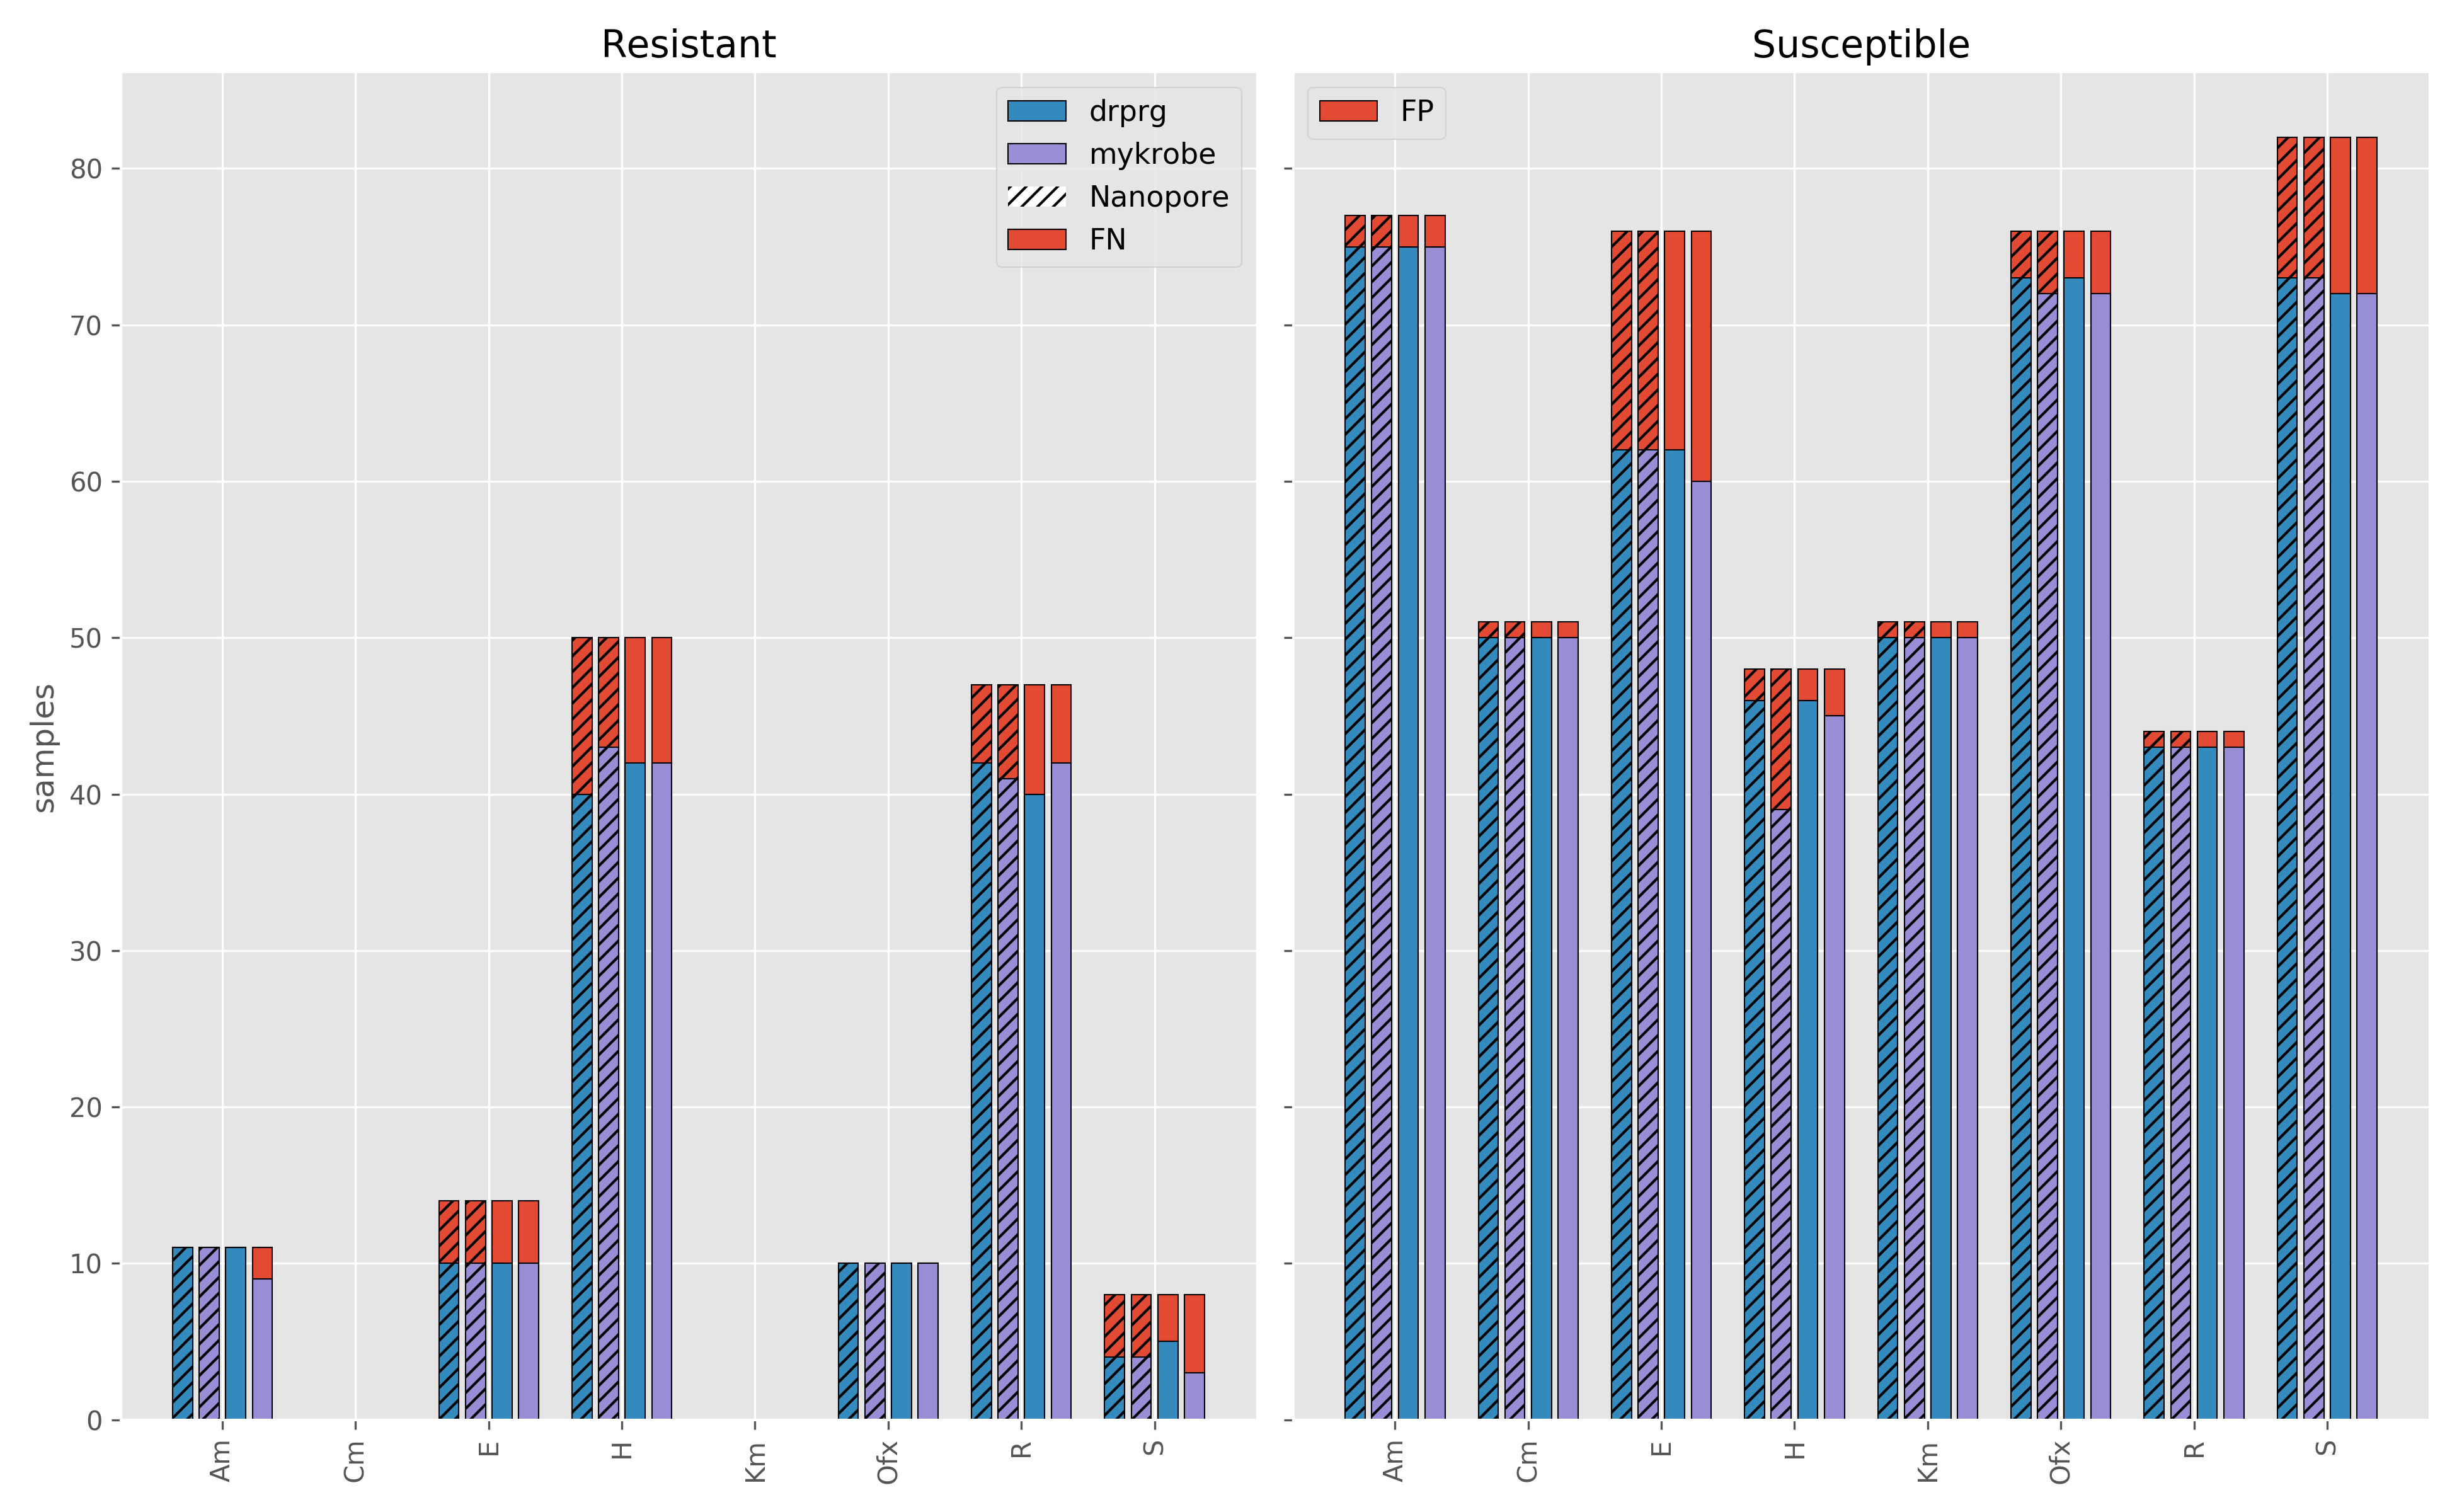
\includegraphics[width=0.90\columnwidth]{Chapter3/Figs/pheno_concordance_plot.png}
\caption{{Number of resistant (left) and susceptible (right) culture-based drug susceptibility testing (DST) phenotypes correctly identified by \mykrobe{} (purple) and \drprg{} (blue) with Illumina (non-striped) and \ont{} (striped) data. The red bars indicate missed (FN) or incorrect (FP) predictions. The x-axis shows the drugs with available phenotype data. E - ethambutol; H - isoniazid; R - rifampicin; S - streptomycin; Km - kanamycin; Am - amikacin; Ofx - ofloxacin; Cm - capreomycin.
{\label{fig:pheno-concordance}}
}}
\end{center}
\end{figure}

These results provide a positive outcome for both our aims. First, \ont{} predictions (striped bars in \autoref{fig:pheno-concordance}) are highly congruent with Illumina. That is, they have equivalent numbers for each classification category. One exception to this is \mykrobe{} \ont{} having noticeably more FPs for isoniazid compared with its Illumina equivalent; all of the extra \ont{} FP calls were indels with no Illumina support. Second, the genome graph-based approach \drprg{}, developed in this chapter, provides predictions consistent with \mykrobe{} - and in some cases, slightly better. 

The most striking and important result from this analysis is the isoniazid FP discrepancy between \mykrobe{} and \drprg{} \ont{} predictions, with 9 and 2 FPs, respectively. As isoniazid is one of the most crucial first-line anti-TB drugs, accurate predictions are critical (\autoref{sec:amr}). Six of the \mykrobe{}-\ont{} isoniazid FPs were caused by erroneous indel calls, which show no support on Illumina, and \drprg{}-\ont{} either had no support or filtered out the call due to poor support. An interesting (but not surprising) observation is that all of these indels occur at homopolymer sites.

Ethambutol and streptomycin had many more FPs and FNs compared to the other drugs for both prediction tools. On further investigation, all ethambutol FPs contain strong evidence for a non-synonymous mutation at codon 306 in \textit{embB}, which is strongly linked to drug resistance \cite{Maningi2017,Srivastava2009,Brossier2015}. Of the 14 samples with FP ethambutol calls (16 for \mykrobe{}-Illumina), six additionally had LPA phenotypes. In all cases, the LPA disagreed with the culture-based phenotype (i.e., LPA was resistant and culture was susceptible). In addition, half of the FNs also have LPA phenotypes available, and both of these cases differed from the culture-based phenotype. When taken together, this information would suggest that the culture-based phenotype for ethambutol \emph{may} be wrong in most of these erroneous cases. However, as highlighted in \autoref{sec:amr}, we stress that while LPA is predictive of resistance, it cannot be used as a means for inferring susceptibility. Therefore, some phenotype-LPA discrepancies may be mutations missing from the LPA catalogue or phenotype minimum inhibitory concentrations (MICs) being close to the cut-off for resistance.

Perhaps the most concerning result from this analysis is the high FNR on isoniazid. However, this is not limited to \ont{} predictions. It is difficult to pinpoint the reasons for missed resistance as there is no way of knowing which mutations we expect to find. There were six samples for which all tool-modality combinations missed resistance. Interestingly, four of these six also had FN calls for rifampicin (accounting for nearly all of the rifampicin FNs). Additionally, 3/10 \drprg{}-\ont{} FNs were missed due to (FRS) filtering of the \textit{fabG1} promoter mutation C-15X, a mutation that has been known to cause phenotype discrepancies before \cite{cryptic2018}. Given the consistent missed resistance across sequencing modalities, the most probable cause of the FNs is an incomplete catalogue. Not all resistance-causing mutations are known, and thus, there will always be limitations to such a panel.

The high streptomycin false-negative rate for all tools and technologies is challenging to account for, as we do not know which resistance-causing mutations we are expected to find. However, manual assessment of the prediction VCFs produced by \drprg{}, and the individual calls by \mykrobe{}, show there is evidence for known resistance-causing mutations in 4/6 cases. One of those is the mutation K88M in \textit{rpsL} which is not in our panel but has been linked to drug resistance previously \cite{Smittipat2016}. While the other FNs were filtered out either due to low coverage or strand bias. Given the low number of streptomycin-resistant samples (8) in this dataset, it is inappropriate to make any claims about the ability to detect resistance for this drug here.

The results from our genome graph-based tool \drprg{} are very positive. There were only two drug/technology situations where \drprg{} had more errors than \mykrobe{}; isoniazid/\ont{}, with \drprg{} having 10 FNs and \mykrobe{} 7; rifampicin/Illumina, with \drprg{} having 7 FNs and \mykrobe{} 5. For all other drug/technology combinations, \drprg{} has equivalent, or less, errors compared to \mykrobe{}.

\begin{table}
\centering
\resizebox{\textwidth}{!}{%
\begin{tabular}{@{}lllllllll@{}}
\toprule
Drug & Technology                & Tool       & FN(R) & FP(S)  & FNR(95\% CI)                  & FPR(95\% CI)         & PPV(95\% CI)         & NPV(95\% CI)           \\ \midrule
\multirow{4}{*}{Amikacin} &
  \multirow{2}{*}{Illumina} &
  \drprg{} &
  0(11) &
  2(77) &
  0.0\% (0.0-25.9\%) &
  2.6\% (0.7-9.0\%) &
  84.6\% (57.8-95.7\%) &
  100.0\% (95.1-100.0\%) \\
     &                           & \mykrobe{} & 2(11) & 2(77)  & \textbf{18.2\% (5.1-47.7\%)}  & 2.6\% (0.7-9.0\%)    & 81.8\% (52.3-94.9\%) & 97.4\% (91.0-99.3\%)   \\
     & \multirow{2}{*}{Nanopore} & \drprg{}   & 0(11) & 2(77)  & 0.0\% (0.0-25.9\%)            & 2.6\% (0.7-9.0\%)    & 84.6\% (57.8-95.7\%) & 100.0\% (95.1-100.0\%) \\
     &                           & \mykrobe{} & 0(11) & 2(77)  & 0.0\% (0.0-25.9\%)            & 2.6\% (0.7-9.0\%)    & 84.6\% (57.8-95.7\%) & 100.0\% (95.1-100.0\%) \\ \cmidrule(l){3-9} 
\multirow{4}{*}{Capreomycin} &
  \multirow{2}{*}{Illumina} &
  \drprg{} &
  0(0) &
  1(51) &
  - &
  2.0\% (0.3-10.3\%) &
  0.0\% (0.0-79.3\%) &
  100.0\% (92.9-100.0\%) \\
     &                           & \mykrobe{} & 0(0)  & 1(51)  & -                             & 2.0\% (0.3-10.3\%)   & 0.0\% (0.0-79.3\%)   & 100.0\% (92.9-100.0\%) \\
     & \multirow{2}{*}{Nanopore} & \drprg{}   & 0(0)  & 1(51)  & -                             & 2.0\% (0.3-10.3\%)   & 0.0\% (0.0-79.3\%)   & 100.0\% (92.9-100.0\%) \\
     &                           & \mykrobe{} & 0(0)  & 1(51)  & -                             & 2.0\% (0.3-10.3\%)   & 0.0\% (0.0-79.3\%)   & 100.0\% (92.9-100.0\%) \\ \cmidrule(l){3-9} 
\multirow{4}{*}{Ethambutol} &
  \multirow{2}{*}{Illumina} &
  \drprg{} &
  4(14) &
  14(76) &
  28.6\% (11.7-54.6\%) &
  \textbf{18.4\% (11.3-28.6\%)} &
  41.7\% (24.5-61.2\%) &
  93.9\% (85.4-97.6\%) \\
     &                           & \mykrobe{} & 4(14) & 16(76) & 28.6\% (11.7-54.6\%)          & 21.1\% (13.4-31.5\%) & 38.5\% (22.4-57.5\%) & 93.8\% (85.0-97.5\%)   \\
 &
  \multirow{2}{*}{Nanopore} &
  \drprg{} &
  4(14) &
  14(76) &
  28.6\% (11.7-54.6\%) &
  18.4\% (11.3-28.6\%) &
  41.7\% (24.5-61.2\%) &
  93.9\% (85.4-97.6\%) \\
     &                           & \mykrobe{} & 4(14) & 14(76) & 28.6\% (11.7-54.6\%)          & 18.4\% (11.3-28.6\%) & 41.7\% (24.5-61.2\%) & 93.9\% (85.4-97.6\%)   \\ \cmidrule(l){3-9} 
\multirow{4}{*}{Isoniazid} &
  \multirow{2}{*}{Illumina} &
  \drprg{} &
  8(50) &
  2(48) &
  16.0\% (8.3-28.5\%) &
  \textbf{4.2\% (1.2-14.0\%)} &
  95.5\% (84.9-98.7\%) &
  85.2\% (73.4-92.3\%) \\
     &                           & \mykrobe{} & 8(50) & 3(48)  & 16.0\% (8.3-28.5\%)           & 6.2\% (2.1-16.8\%)   & 93.3\% (82.1-97.7\%) & 84.9\% (72.9-92.1\%)   \\
 &
  \multirow{2}{*}{Nanopore} &
  \drprg{} &
  10(50) &
  2(48) &
  \textbf{20.0\% (11.2-33.0\%)} &
  \textbf{4.2\% (1.2-14.0\%)} &
  \textbf{95.2\% (84.2-98.7\%)} &
  82.1\% (70.2-90.0\%) \\
     &                           & \mykrobe{} & 7(50) & 9(48)  & 14.0\% (7.0-26.2\%)           & 18.8\% (10.2-31.9\%) & 82.7\% (70.3-90.6\%) & 84.8\% (71.8-92.4\%)   \\ \cmidrule(l){3-9} 
\multirow{4}{*}{Kanamycin} &
  \multirow{2}{*}{Illumina} &
  \drprg{} &
  0(0) &
  1(51) &
  - &
  2.0\% (0.3-10.3\%) &
  0.0\% (0.0-79.3\%) &
  100.0\% (92.9-100.0\%) \\
     &                           & \mykrobe{} & 0(0)  & 1(51)  & -                             & 2.0\% (0.3-10.3\%)   & 0.0\% (0.0-79.3\%)   & 100.0\% (92.9-100.0\%) \\
     & \multirow{2}{*}{Nanopore} & \drprg{}   & 0(0)  & 1(51)  & -                             & 2.0\% (0.3-10.3\%)   & 0.0\% (0.0-79.3\%)   & 100.0\% (92.9-100.0\%) \\
     &                           & \mykrobe{} & 0(0)  & 1(51)  & -                             & 2.0\% (0.3-10.3\%)   & 0.0\% (0.0-79.3\%)   & 100.0\% (92.9-100.0\%) \\ \cmidrule(l){3-9} 
\multirow{4}{*}{Ofloxacin} &
  \multirow{2}{*}{Illumina} &
  \drprg{} &
  0(10) &
  3(76) &
  0.0\% (-0.0-27.8\%) &
  3.9\% (1.4-11.0\%) &
  76.9\% (49.7-91.8\%) &
  100.0\% (95.0-100.0\%) \\
     &                           & \mykrobe{} & 0(10) & 4(76)  & 0.0\% (-0.0-27.8\%)           & 5.3\% (2.1-12.8\%)   & 71.4\% (45.4-88.3\%) & 100.0\% (94.9-100.0\%) \\
     & \multirow{2}{*}{Nanopore} & \drprg{}   & 0(10) & 3(76)  & 0.0\% (-0.0-27.8\%)           & 3.9\% (1.4-11.0\%)   & 76.9\% (49.7-91.8\%) & 100.0\% (95.0-100.0\%) \\
     &                           & \mykrobe{} & 0(10) & 4(76)  & 0.0\% (-0.0-27.8\%)           & 5.3\% (2.1-12.8\%)   & 71.4\% (45.4-88.3\%) & 100.0\% (94.9-100.0\%) \\ \cmidrule(l){3-9} 
\multirow{4}{*}{Rifampicin} &
  \multirow{2}{*}{Illumina} &
  \drprg{} &
  7(47) &
  1(44) &
  14.9\% (7.4-27.7\%) &
  2.3\% (0.4-11.8\%) &
  97.6\% (87.4-99.6\%) &
  86.0\% (73.8-93.0\%) \\
     &                           & \mykrobe{} & 5(47) & 1(44)  & 10.6\% (4.6-22.6\%)           & 2.3\% (0.4-11.8\%)   & 97.7\% (87.9-99.6\%) & 89.6\% (77.8-95.5\%)   \\
     & \multirow{2}{*}{Nanopore} & \drprg{}   & 5(47) & 1(44)  & 10.6\% (4.6-22.6\%)           & 2.3\% (0.4-11.8\%)   & 97.7\% (87.9-99.6\%) & 89.6\% (77.8-95.5\%)   \\
     &                           & \mykrobe{} & 6(47) & 1(44)  & 12.8\% (6.0-25.2\%)           & 2.3\% (0.4-11.8\%)   & 97.6\% (87.7-99.6\%) & 87.8\% (75.8-94.3\%)   \\ \cmidrule(l){3-9} 
\multirow{4}{*}{Streptomycin} &
  \multirow{2}{*}{Illumina} &
  \drprg{} &
  3(8) &
  10(82) &
  37.5\% (13.7-69.4\%) &
  12.2\% (6.8-21.0\%) &
  33.3\% (15.2-58.3\%) &
  96.0\% (88.9-98.6\%) \\
     &                           & \mykrobe{} & 5(8)  & 10(82) & \textbf{62.5\% (30.6-86.3\%)} & 12.2\% (6.8-21.0\%)  & 23.1\% (8.2-50.3\%)  & 93.5\% (85.7-97.2\%)   \\
     & \multirow{2}{*}{Nanopore} & \drprg{}   & 4(8)  & 9(82)  & 50.0\% (21.5-78.5\%)          & 11.0\% (5.9-19.6\%)  & 30.8\% (12.7-57.6\%) & 94.8\% (87.4-98.0\%)   \\
     &                           & \mykrobe{} & 4(8)  & 9(82)  & 50.0\% (21.5-78.5\%)          & 11.0\% (5.9-19.6\%)  & 30.8\% (12.7-57.6\%) & 94.8\% (87.4-98.0\%)   \\ \cmidrule(l){3-9} 
\end{tabular}%
}
\caption{Comparison of WGS-based drug resistance prediction concordance with culture-based drug susceptibility testing (DST) phenotypes. For this comparison, we assume the DST phenotype is correct and evaluate the WGS predictions accordingly. \drprg{} and \mykrobe{} are the two tools that provide WGS predictions. Bold text is used to highlight differences of note between \drprg{} and \mykrobe{}. FN=false negative; R=number of resistant samples; FP=false positive; S=number of susceptible samples; FNR=false negative rate; FPR=false positive rate; PPV=positive predictive value; NPV=negative predictive value; CI=Wilson score confidence interval}
\label{tab:pheno-concordance}
\end{table}

\subsection{Summary}

WGS-based drug resistance predictions from \ont{} are as reliable as those from Illumina when compared to culture-based DST phenotypes. Additionally, we have shown that genome graphs provide reliable predictions for both Illumina and \ont{} data using our tool \drprg{}.

While there is a seemingly high number of FNs and FPs for some drugs, many of these errors result from a (\mykrobe{}) \ont{}-related indel issues or the absence of known resistance-causing mutations in the panel. Importantly, missed resistance predictions were not technology-driven and presumably occurred because the catalogue lacks the relevant resistance-causing mutations.

%=========================================================================
\section{Effect of \ont{} read depth}
\label{sec:dst-covg}

An important consideration when performing \ont{} sequencing for AMR prediction is how much data is needed. The quantity of data required has implications for how long the \ont{} sequencing device needs to be run or how many samples can be multiplexed in a single run in order to yield sufficient data for reliable predictions. A previous study by Votintseva \etal{} found that deep coverage is required of \ont{} to predict drug resistance accurately\cite{Votintseva2017}. As \ont{} sequencing advances quickly, and our dataset contains a broad \ont{} depth-of-coverage range (29-150x), we explore whether this requirement of high coverage still holds. 

We binned samples into groups based on their read depth. The groups were segregated into lots of 10x depth. That is, if a sample has a read depth of 56, it is assigned to the 50x bin, which covers samples with read depth less than 60, but $\ge50$. We calculate the proportions of each drug resistance classification (FN, TP, TN, FP) present for each bin. For this analysis, we use the culture-based phenotype classifications from \autoref{sec:pheno-concordance}. If low read depth leads to poor resistance prediction, we would expect the proportions of FPs and FNs in the low-depth bins to be greater than in the high-depth bins. 

As \autoref{fig:pheno-covg} illustrates, we see no relationship between \ont{} read depth and erroneous predictions. Further work at depths lower than 30x is warranted, but this is convincing evidence that samples with "only" 30x \ont{} read depth still yield reliable resistance predictions. 

\begin{figure}
\begin{center}
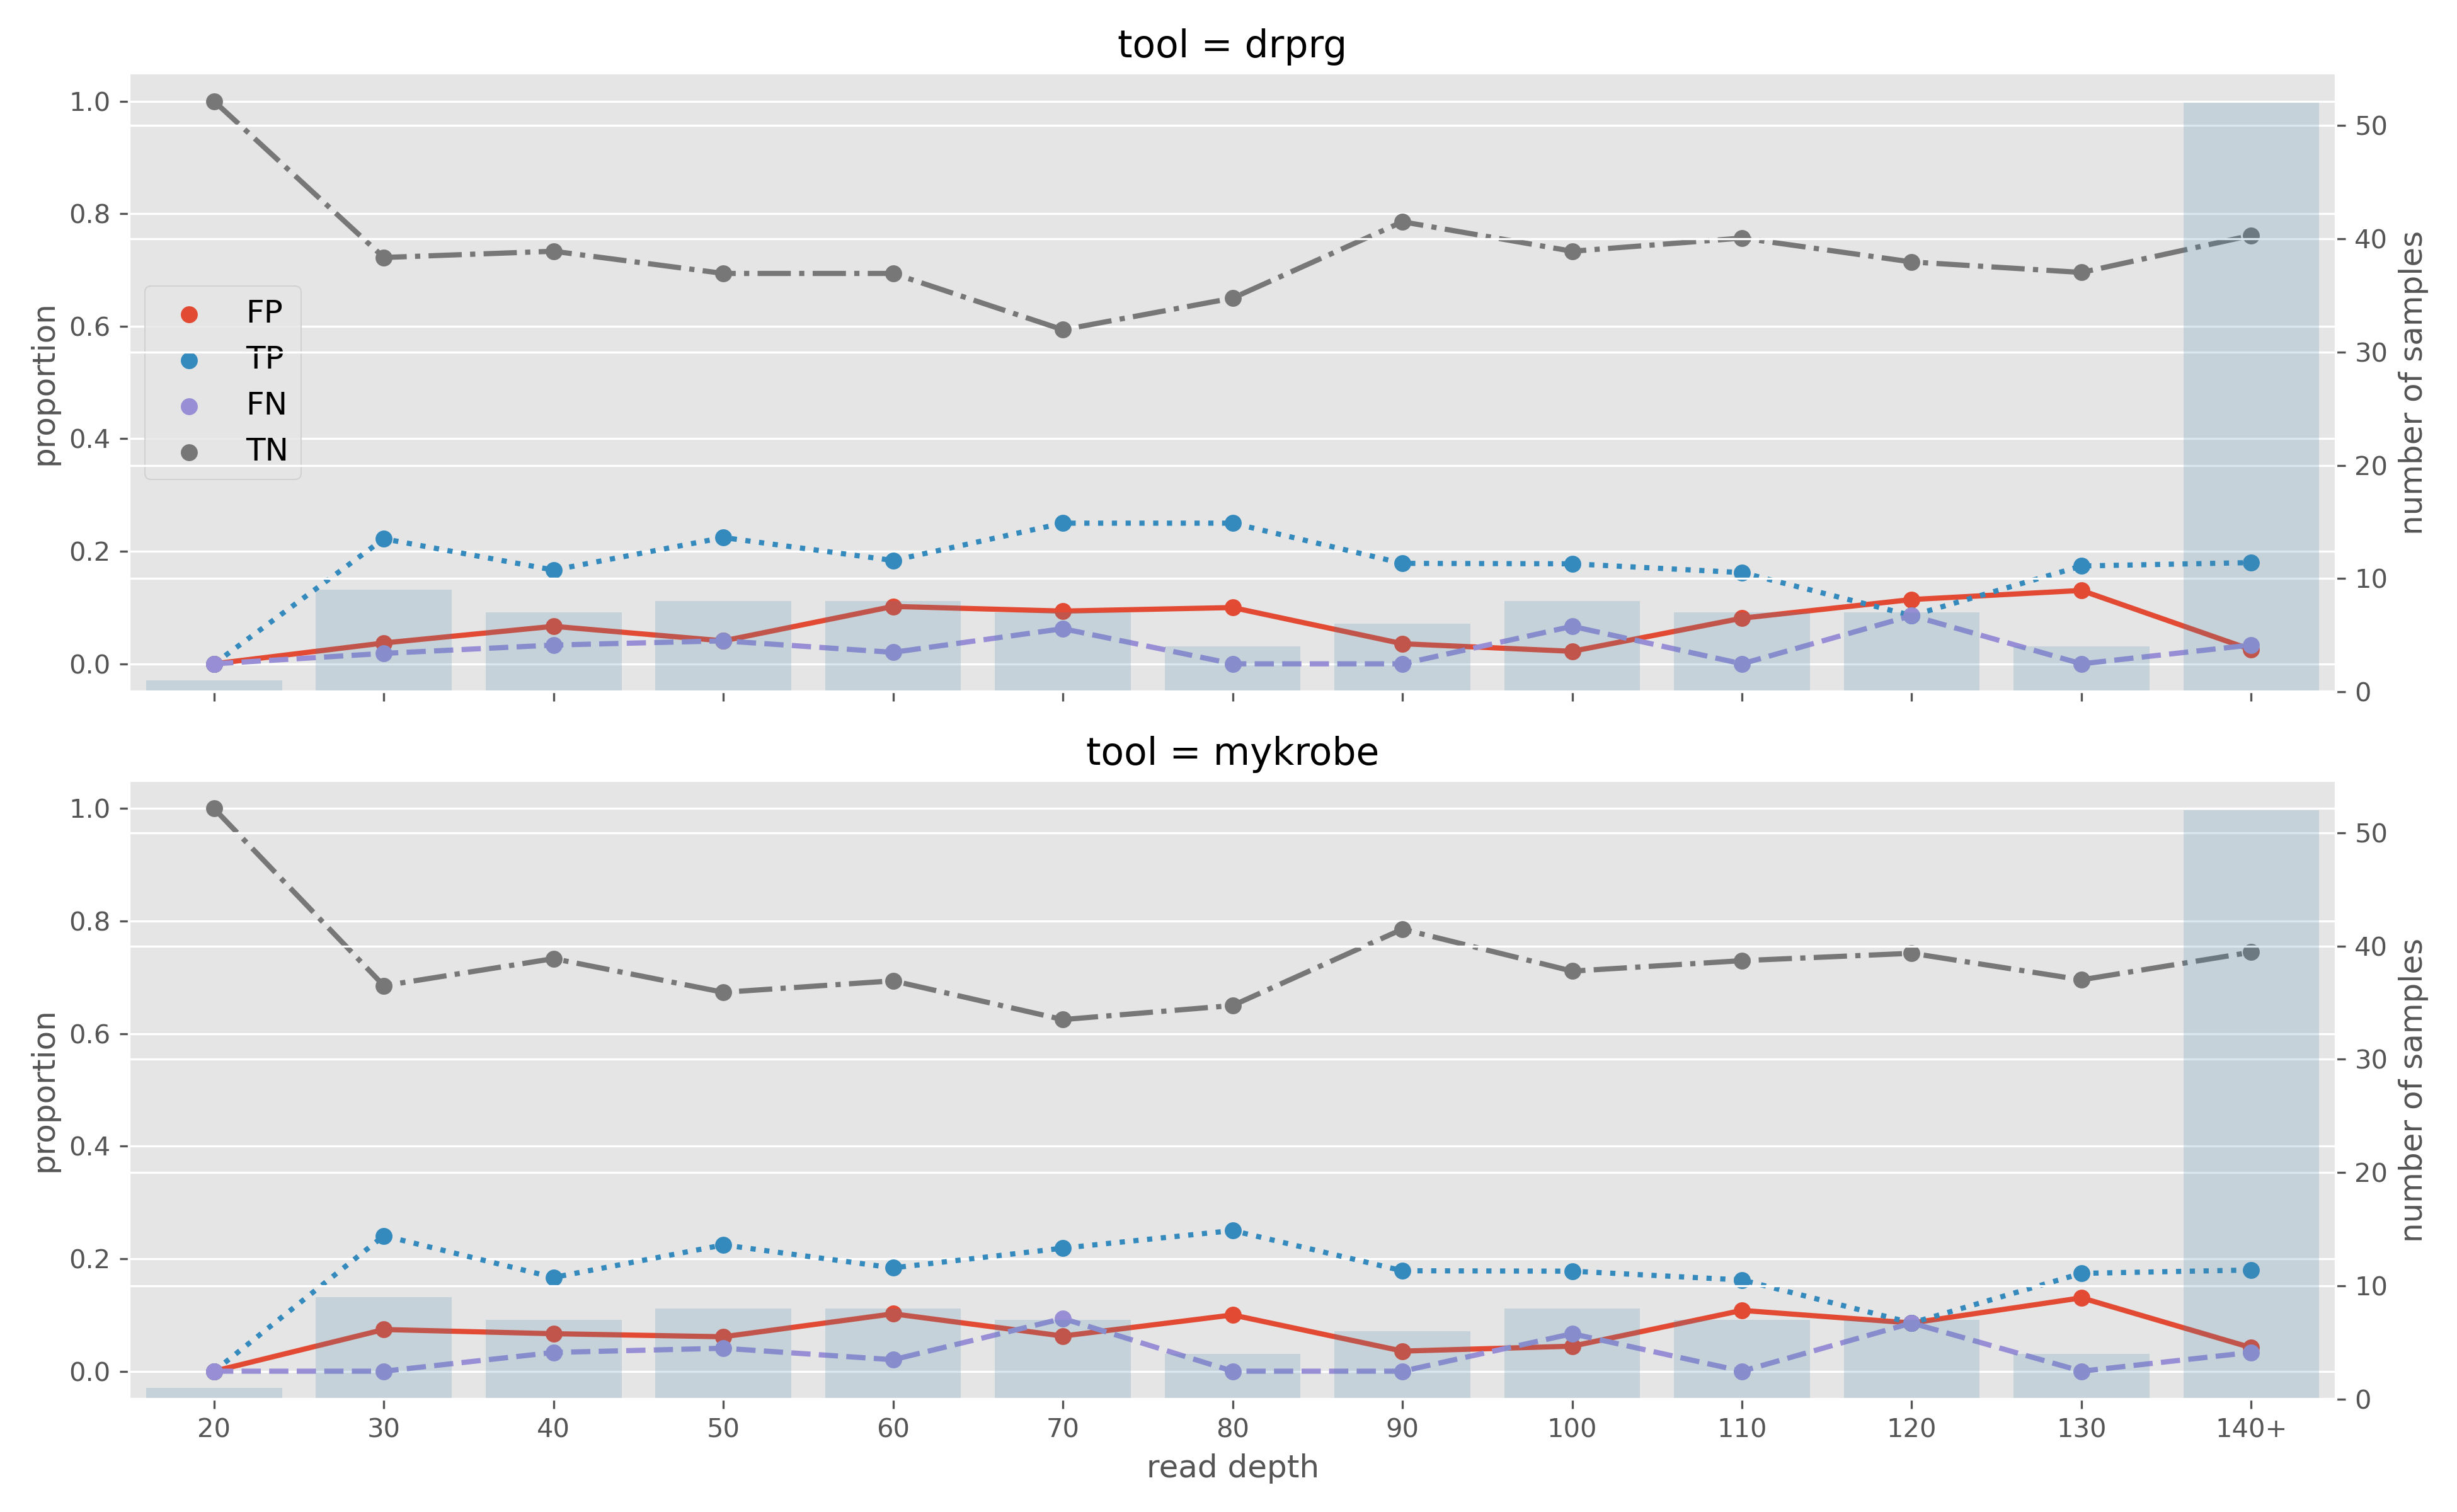
\includegraphics[width=0.90\columnwidth]{Chapter3/Figs/phenotype_coverage.png}
\caption{{Effect of \ont{} read depth on \drprg{} (top) and \mykrobe{} (bottom) drug susceptibility phenotype prediction. Each point indicates the proportion (left y-axis) of classifications of that type at the read depth (x-axis). Read depth is binned such that 40 is all samples with a read depth $\ge40$ and less than 50. The blue bars indicate the number of samples (right y-axis) contained in each bin. FP=false positive (red); TN=true negative (grey); FN=false negative (purple); TP=true positive (blue).
{\label{fig:pheno-covg}}
}}
\end{center}
\end{figure}
%=========================================================================
\section{Detecting off-catalogue mutations}
\label{sec:drprg-discover}

One of the main advantages \drprg{} has over \mykrobe{} is the ability to discover off-catalogue (novel) variants. The reason \drprg{} can call mutations outside of the panel is that it uses \pandora{} as the underlying method for producing predictions from sequencing reads.

The \cryptic{} Consortium have shown that refusing to make predictions in the case where a non-panel variant is discovered in a resistance-associated gene can improve pan-susceptibility prediction by reducing missed resistance (FN) calls \cite{cryptic2018}. However, that work focused only on first-line drugs and did not detail the variants discovered. 

In this section, we aim to assess the novel variant detection capacity of \drprg{} on both Illumina and \ont{} data. While this study is underpowered to make pan-susceptibility predictions, we have a dataset with well-characterised SNPs from \autoref{chap:denovo}. These high-quality variant calls give us a way of determining how many SNPs \drprg{} finds and misses in resistance-associated genes. 

We remove any position in the COMPASS SNPs VCF from \autoref{sec:illumina-var-call} that falls into one of three categories: i) does not occur inside any mutation catalogue gene; ii) does not call an alternate allele; or iii) exists in the panel. After this filtering, we have a VCF containing SNPs in resistance-associated genes that do not occur in the panel - referred to as the truth VCF.

We classify the novel SNPs called by \drprg{} against the truth VCF using \vrb{hap.py} - a VCF comparison program developed by Illumina and the Global Alliance for Genomics and Health Benchmarking Team \cite{happy2019}. \autoref{fig:novel-classifications} and \autoref{tab:novel-classifications} show the number of TP, FP, and FN novel SNP calls made by \drprg{} for each drug across all 150 samples. 

From \autoref{fig:novel-classifications} we clearly see \textit{rpoB} contains the most off-panel SNPs. Of particular note is the large percentage of \textit{gyrA} FNs, which leads to a recall of 0.35 for both Illumina and \ont{} in this gene. Upon further investigation, all of these missed calls were filtered out by \drprg{} due to low FRS. Additionally, we see the same scenario when looking at the \textit{ahpC} FNs - which are much higher in \ont{} data. 

Despite the poor recall in \textit{gyrA} and \textit{ahpC}, the precision of novel \drprg{} calls is encouraging. In total, there were two FPs detected in \textit{rpoB} (for both technologies), and one \ont{} FP in \textit{rrs}. This result suggests we can be very confident in the novel SNP calls made by \drprg{}.

\begin{figure}
\begin{center}
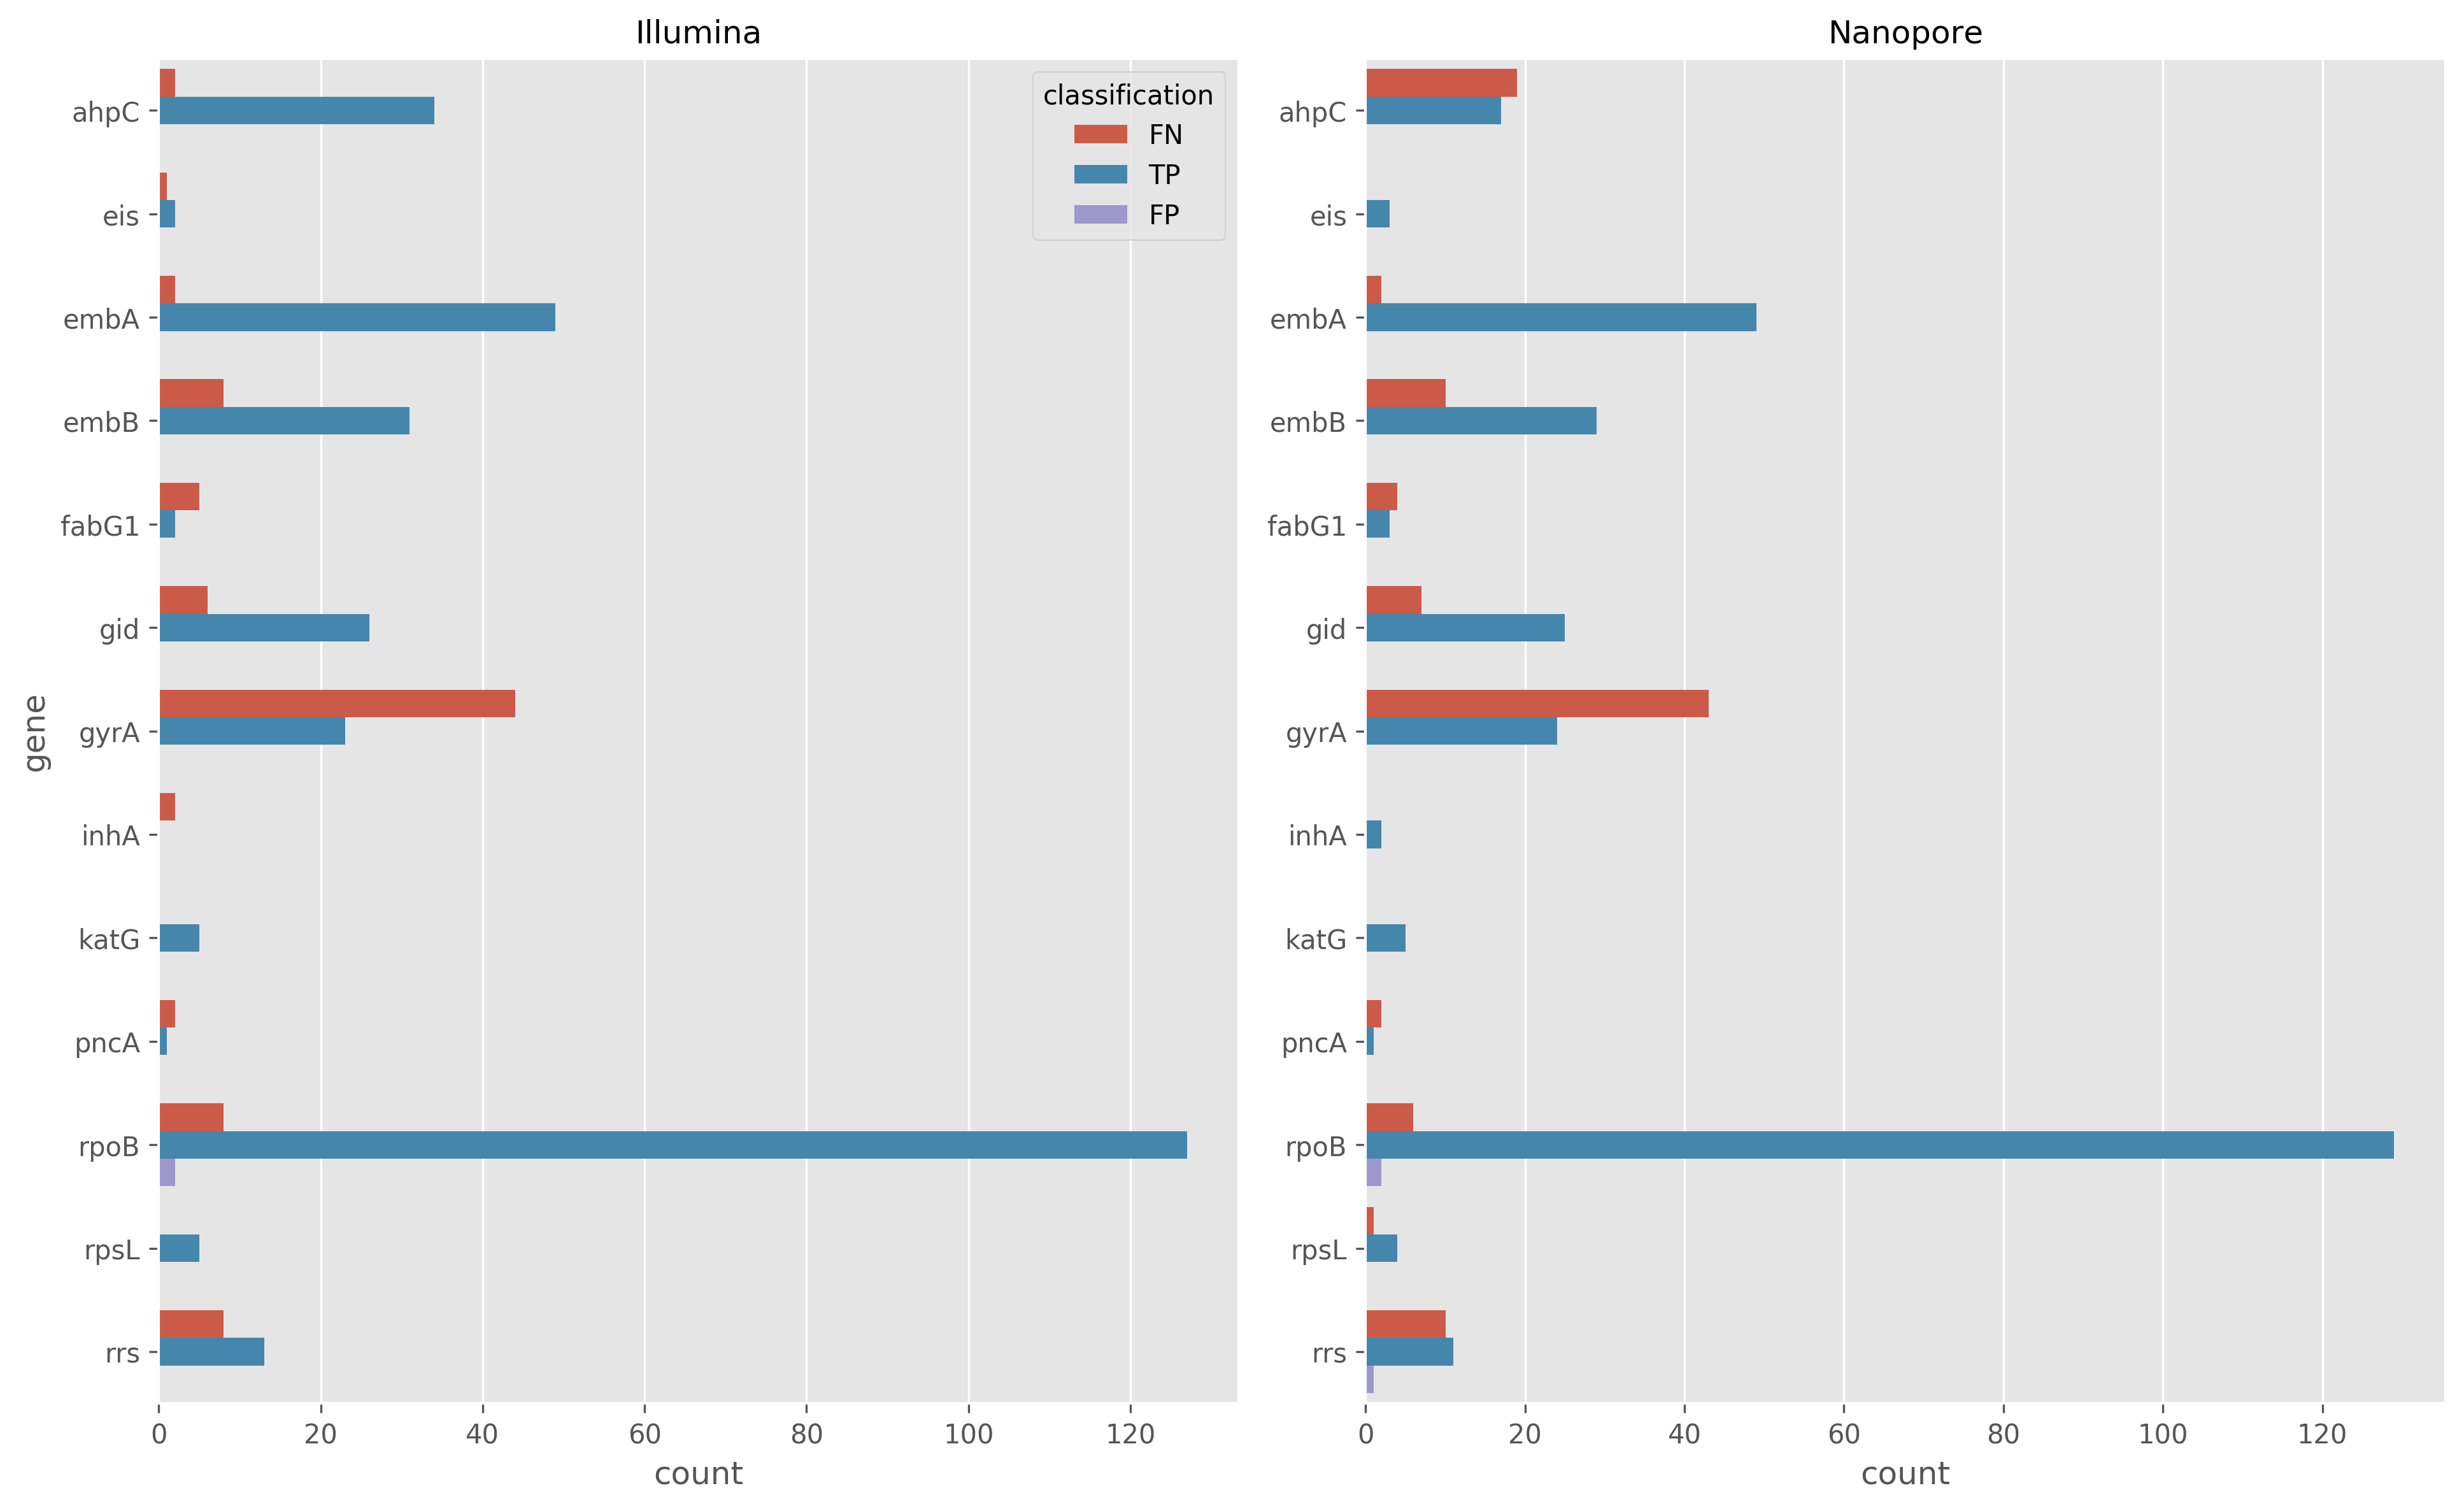
\includegraphics[width=0.90\columnwidth]{Chapter3/Figs/novel_classifications.png}
\caption{{Classifications of novel SNP calls made from Illumina (left) and \ont{} (right) data by \drprg{} in resistance-associated genes (y-axis). Counts (x-axis) are across all samples. TP (blue) - true positive; FN (red) - false negative; FP (purple) - false positive.
{\label{fig:novel-classifications}}
}}
\end{center}
\end{figure}

\begin{table}
\centering
\begin{tabular}{@{}lllllll@{}}
\toprule
Gene                            & Technology & FN & FP & TP  & Recall & Precision \\ \midrule
\multirow{2}{*}{\textit{ahpC}}  & Illumina   & 2  & 0  & 34  & 0.944  & 1.000     \\
                                & \ont{}     & 19 & 0  & 17  & 0.472  & 1.000     \\ \cmidrule(l){2-7}
\multirow{2}{*}{\textit{eis}}   & Illumina   & 1  & 0  & 2   & 0.667  & 1.000     \\
                                & \ont{}     & 0  & 0  & 3   & 1.000  & 1.000     \\ \cmidrule(l){2-7}
\multirow{2}{*}{\textit{embA}}  & Illumina   & 2  & 0  & 49  & 0.961  & 1.000     \\
                                & \ont{}     & 2  & 0  & 49  & 0.961  & 1.000     \\ \cmidrule(l){2-7}
\multirow{2}{*}{\textit{embB}}  & Illumina   & 8  & 0  & 31  & 0.795  & 1.000     \\
                                & \ont{}     & 10 & 0  & 29  & 0.744  & 1.000     \\ \cmidrule(l){2-7}
\multirow{2}{*}{\textit{fabG1}} & Illumina   & 5  & 0  & 2   & 0.286  & 1.000     \\
                                & \ont{}     & 4  & 0  & 3   & 0.429  & 1.000     \\ \cmidrule(l){2-7}
\multirow{2}{*}{\textit{gid}}   & Illumina   & 6  & 0  & 26  & 0.812  & 1.000     \\
                                & \ont{}     & 7  & 0  & 25  & 0.781  & 1.000     \\ \cmidrule(l){2-7}
\multirow{2}{*}{\textit{gyrA}}  & Illumina   & 44 & 0  & 23  & 0.343  & 1.000     \\
                                & \ont{}     & 43 & 0  & 24  & 0.358  & 1.000     \\ \cmidrule(l){2-7}
\multirow{2}{*}{\textit{inhA}}  & Illumina   & 2  & 0  & 0   & 0.000  & -         \\
                                & \ont{}     & 0  & 0  & 2   & 1.000  & 1.000     \\ \cmidrule(l){2-7}
\multirow{2}{*}{\textit{katG}}  & Illumina   & 0  & 0  & 5   & 1.000  & 1.000     \\
                                & \ont{}     & 0  & 0  & 5   & 1.000  & 1.000     \\ \cmidrule(l){2-7}
\multirow{2}{*}{\textit{pncA}}  & Illumina   & 2  & 0  & 1   & 0.333  & 1.000     \\
                                & \ont{}     & 2  & 0  & 1   & 0.333  & 1.000     \\ \cmidrule(l){2-7}
\multirow{2}{*}{\textit{rpoB}}  & Illumina   & 8  & 2  & 127 & 0.941  & 0.984     \\
                                & \ont{}     & 6  & 2  & 129 & 0.956  & 0.985     \\ \cmidrule(l){2-7}
\multirow{2}{*}{\textit{rpsL}}  & Illumina   & 0  & 0  & 5   & 1.000  & 1.000     \\
                                & \ont{}     & 1  & 0  & 4   & 0.800  & 1.000     \\ \cmidrule(l){2-7}
\multirow{2}{*}{\textit{rrs}}   & Illumina   & 8  & 0  & 13  & 0.619  & 1.000     \\
                                & \ont{}     & 10 & 1  & 11  & 0.524  & 0.917     \\ \cmidrule(l){2-7} 
\end{tabular}
\caption{Classification of novel SNP calls made by \drprg{} in resistance-associated genes. Counts are across all samples. TP - true positive; FN - false negative; FP - false positive.}
\label{tab:novel-classifications}
\end{table}

\autoref{fig:novel-sample-classifications} illustrates the number of novel calls of different classification on a per-sample basis. It shows that on average, a samples will have 2 novel TP calls and 0 FPs and FNs. 

\begin{figure}
\begin{center}
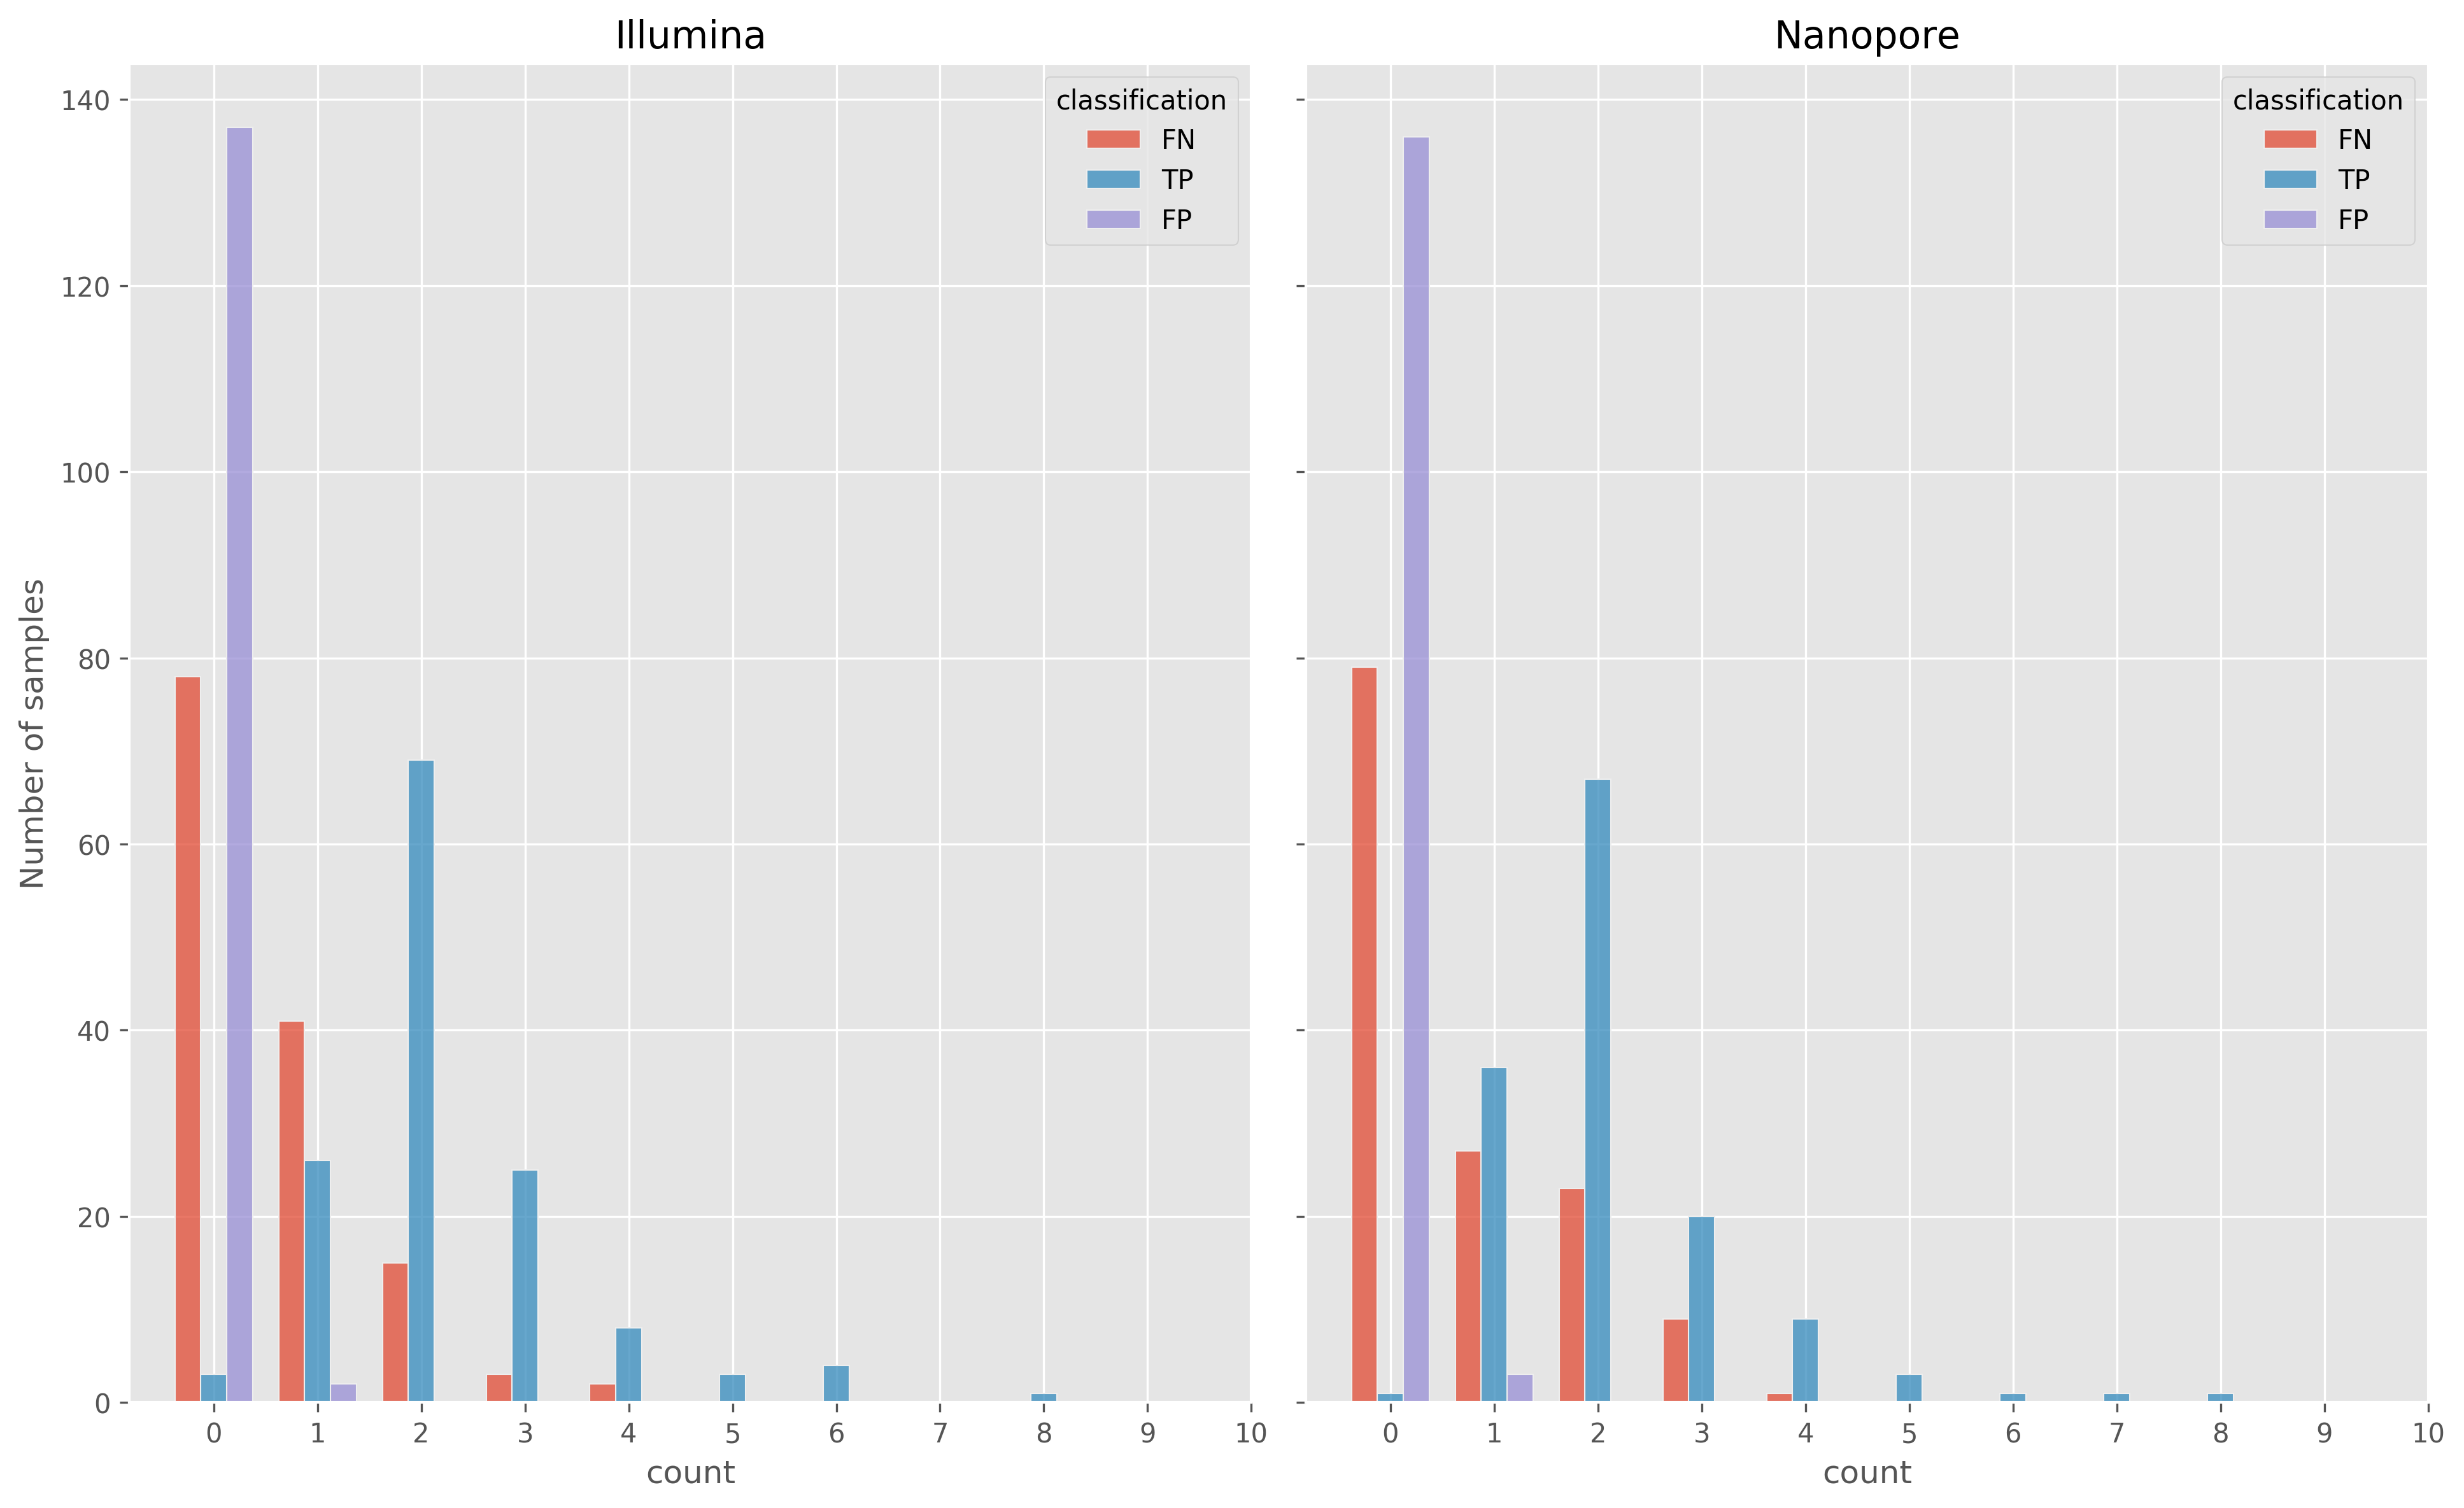
\includegraphics[width=0.90\columnwidth]{Chapter3/Figs/novel_classifications_per_sample.png}
\caption{{Number of novel variants found in resistance-associated genes for each sample. The x-axis indicates the number of classifications of the relevant kind for a sample, and the y-axis is the number of samples with that classification count. The classifications are: TP (blue) - true positive; FN (red) - false negative; FP (purple) - false positive.
{\label{fig:novel-sample-classifications}}
}}
\end{center}
\end{figure}

Having seen that the off-panel SNPs called by \drprg{} are precise, we look at how incorporating this information impacts the AMR predictions. \autoref{fig:pheno-unknown} is the same as \autoref{fig:pheno-concordance}, except with unknown (off-panel) calls included. If we find a novel variant, an unknown prediction is given for the drug(s) associated with that gene. The exception to this is when a known resistance-causing mutation is also found for the respective drug(s), in which case a resistant prediction is made.

Of note in \autoref{fig:pheno-unknown} is the reduced number of missed resistance calls made when we include unknown variants - when compared to \autoref{fig:pheno-concordance}. That is, a call of unknown is our way of indicating to the user that we did not find a \emph{known} resistance-causing mutation; however, we did find a mutation that is not known to be either resistance- or susceptibility-associated.

While we see a reduction in the number of missed resistance calls (FN) when calling unknown variants, the number of definitive susceptibility (TN) calls is also reduced. However, these are not "missed" susceptibility calls and would just require phenotyping more samples (a situation preferred by many clinicians in response to \cite{hunt2019}). In particular, ethambutol, rifampicin, and streptomycin see a large number of unknown calls. A large number of unknown calls for rifampicin is not unexpected as \textit{rpoB} (associated with rifampicin resistance) had by far the most novel variants in the above analysis (\autoref{fig:novel-classifications}). Nearly every one of these unknown rifampicin calls relates to synonymous mutations D103D (C309T) and A1075A (T3225C) that are known not to be associated with drug resistance \cite{Jagielski2018}. Likewise, synonymous mutations were also the cause of the bulk of unknown calls for other drugs. However, there were some indel calls found. As our truth VCF only contains SNPs, we cannot assess the validity of these indel calls.

A simple solution for the excessive unknown calls in susceptible samples would include synonymous mutations in the panel as susceptibility-associated.

\begin{figure}
\begin{center}
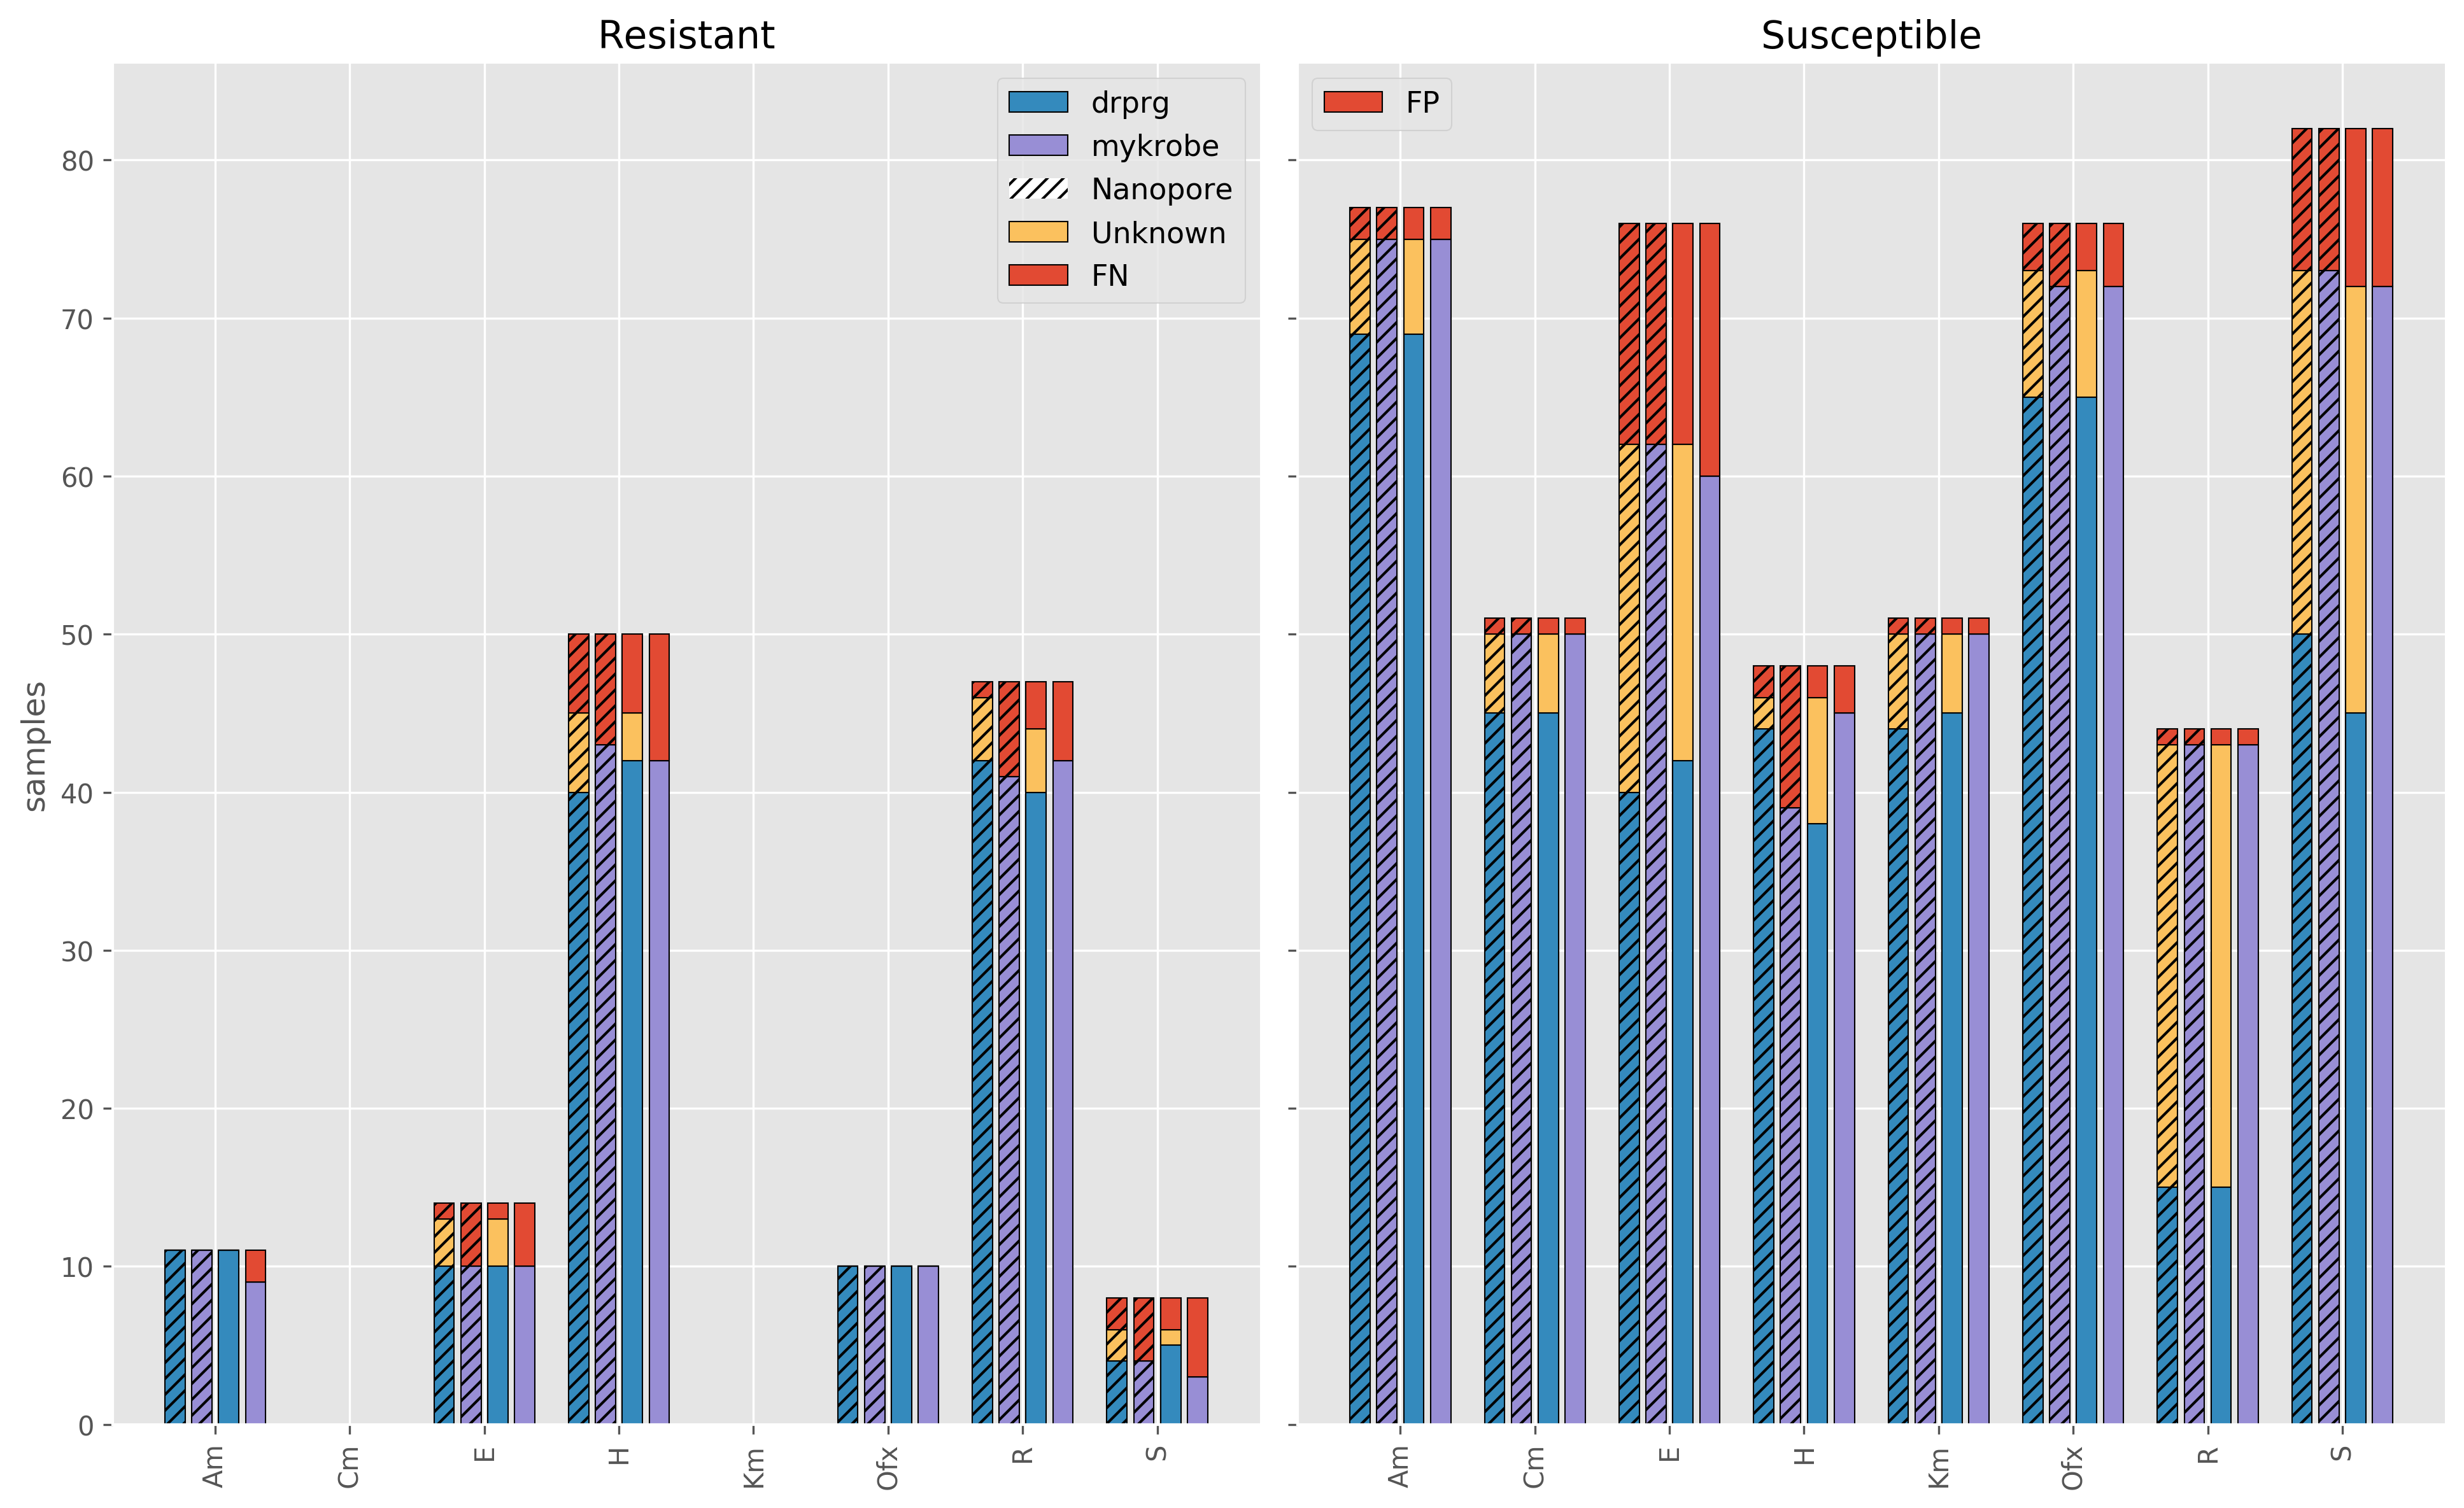
\includegraphics[width=0.90\columnwidth]{Chapter3/Figs/pheno_unknown.png}
\caption{{Number of resistant (left) and susceptible (right) culture-based drug susceptibility testing (DST) phenotypes correctly identified by \mykrobe{} (purple) and \drprg{} (blue) with Illumina (non-striped) and \ont{} (striped) data. The red bars indicate missed (FN) or incorrect (FP) predictions. The yellow bars represent \drprg{} "unknown" calls, which is when there is an off-panel variant found in a gene associated with the respective drug. If there is no resistance-associated variant found for that drug, then an unknown call is made. The x-axis shows the drugs with available phenotype data. E - ethambutol; H - isoniazid; R - rifampicin; S - streptomycin; Km - kanamycin; Am - amikacin; Ofx - ofloxacin; Cm - capreomycin.
{\label{fig:pheno-unknown}}
}}
\end{center}
\end{figure}

\subsection{Summary}

Producing unknown drug resistance predictions based on novel variant calls is a point of difference for \drprg{}. In this section, we have shown that novel variants detected by \drprg{} are precise, but that missed calls require some more work.

We have also shown that we can reduce missed resistance calls by refusing to make predictions for drugs with variants of unknown consequences. However, this currently comes at the cost of fewer susceptibility calls, which means sending more samples for phenotyping, but not missing susceptibility. Although, an easy fix for many of these susceptible samples sent for phenotyping - incorporating synonymous mutations - has been identified.

%=========================================================================
\section{Discussion}
Illumina WGS has become a standard tool for \mtb{} drug susceptibility testing. Its use is underpinned by a vast number of studies validating the sensitivity and specificity of such predictions, all with similar results \cite{cryptic2018,hunt2019,bradley2015,coll2015,walker2015,kohl2018,phelan2019}. In this chapter, we have provided evidence that \ont{} WGS-based DST can provide predictions consistent with Illumina. We did this by showing that when comparing \ont{}-predicted phenotypes to those from Illumina-predicted and culture-based phenotypes, there is very little difference between the predictions from the two technologies. However, for isoniazid, we do note a significantly higher \ont{} false positive rate (18.8\%) than Illumina (6.2\%) when using \mykrobe{} - but we offer a solution to this below.

In addition to validating the use of \ont{} for DST, we also developed and evaluated a software tool \drprg{} for the same task. Many programs exist to predict drug resistance from WGS data; however, all have the same underlying limitation: an inability to detect off-panel (novel) mutations. With \drprg{} we have made a first step in removing this limitation from \mtb{} AMR prediction.

\drprg{} is not the first tool to use the concept of genome graphs for AMR prediction. \mykrobe{}, the other tool used in this chapter, uses population genome graphs for genotyping of samples. The underlying method \mykrobe{} uses is Cortex \cite{iqbal2012} - a program that uses coloured de Bruijn graphs for genotyping samples via \denovo{} assembly. Cortex is somewhat of a precursor to \pandora{} - the genome graph method underpinning \drprg{}. However, \pandora{} offers a number of advantages over Cortex (see \autoref{sec:genome-graphs-dst} for a full description of these). Ultimately, the differences mean, theoretically, \pandora{} (\drprg{}) requires less read depth to produce the same information as Cortex (\mykrobe{}) and is much better suited to use with noisy, error-prone \ont{} data. 

When comparing the computational performance of \mykrobe{} and \drprg{}, we found \drprg{} to be faster and more memory efficient for both technologies (\autoref{sec:drprg-comp-perf}).

\hspace{0.75cm}

\noindent
Given the extensive validation of Illumina WGS for DST, with many more samples than we have in this chapter, our intention is not to assert the clinical use of WGS. Instead, we seek to gauge \ont{}'s suitability for WGS-based DST. 

As \mykrobe{} has been extensively validated on large datasets with Illumina \cite{bradley2015,hunt2019}, using it as a truth to compare \ont{} to provides evidence for \ont{}'s use for AMR prediction. We performed this analysis in \autoref{sec:geno-concordance} and found \mykrobe{}'s \ont{} predictions to be highly concordant with those from Illumina. There were only eight missed resistance calls, seven of which were minor resistance calls on Illumina. We attempted to allow minor resistance calls for \ont{}, but this led to every sample being predicted as resistant to isoniazid and pyrazinamide due to false heterozygous indel calls in \textit{katG} and \textit{pncA}. Of the false-positive calls made by \mykrobe{} on \ont{} data, half were due to indel calls in \textit{katG}, while the other half are quite likely (SNP) errors on behalf of Illumina due to filtering.

When comparing the \drprg{} predictions to \mykrobe{} Illumina profiles, we see somewhat similar results. As with \mykrobe{}-\ont{} errors, almost all \drprg{}-\ont{} errors were due to indel calls in \textit{katG} and \textit{pncA}, while the rest were most likely \mykrobe{}-Illumina errors, as mentioned above. 

\noindent
We next assessed Illumina and \ont{} predictions against "gold-standard" culture-based phenotypic testing in \autoref{sec:pheno-concordance}. This analysis allows an unbiased assessment of the two sequencing modalities, intending to detect any technology-driven differences. As all our samples were sequenced from the same DNA extraction, we know the resistance profile for the underlying data is the same for both technologies. 

\ont{} has been assessed for use in providing AMR predictions previously \cite{bradley2015,hunt2019,phelan2019}, but with single-digit sample sizes. An exception to this is the work by the New York State Department of Health, which used a sample size of 431 \cite{smith2020}. Our results from \autoref{sec:pheno-concordance} are in agreement with all of these previous studies; \ont{} AMR predictions are highly concordant with Illumina when compared to culture-based phenotypes - using our altered parameters from \autoref{app:mykrobe-settings}. This agreement is found for both \mykrobe{} and \drprg{}. As mentioned, the one exception to this was \mykrobe{}'s \ont{} isoniazid predictions, which had a higher false-positive rate compared to the other technology/tool combinations. All of these extra FPs were due to \textit{katG} indel calls in the \ont{} data, which as mentioned, is a systematic problem currently affecting \ont{} \cite{watson2019}. One point of difference between the \ont{} study by Smith \etal{} and ours is that our dataset is from three countries with very different \mtb{} populations, whilst Smith \etal{} use a more homogeneous population from New York state. 

While there is a high level of similarity between predictions from both tools and sequencing modalities, disagreement with the culture-based phenotype is high for some drugs. For example, isoniazid FNR of 14-20\% is higher than previous work \cite{hunt2019,cryptic2018}. In almost all of these errors, we see strong evidence for mutations previously linked to drug resistance, but not in our panel. These discrepancies raise the ongoing need for a curated panel of known mutations and their impacts on susceptibility. 

The ethambutol false negative rate (FNR; 28.6\%) was much higher than previous reports, which generally fall in the 5-10\% range \cite{cryptic2018,hunt2019,smith2020}. However, Smith \etal{} did see an FNR of 20\%. In addition, the positive predictive value (PPV; also known as precision) was 41.7\%, again, much lower than previous studies. However, all FP predictions were made due to a non-synonymous mutation at codon 306 in \textit{embB}. We saw consistent support for the presence of these FP mutations on all technologies and tools, and multiple previous reports have strongly linked this mutation to ethambutol resistance \cite{Maningi2017,Srivastava2009,Brossier2015}. Additionally, phenotyping of isolates with this particular mutation is known to be unreliable \cite{Zhang2014,walker2015,Sirgel2013}, raising the possibility of a spurious culture-based phenotype in these cases. Indeed, sequencing of the resistance-associated genes is now recommended over culture-based phenotyping for ethambutol \cite{who2018technical}.

The main limitation for this section of the chapter is the number of resistant samples. Although there was 50 isoniazid- and 47 rifampicin-resistant isolates, the other drugs had no more than 15 samples representing. The low number of resistant samples is reflected in the breadth of confidence intervals for all drugs. However, combining this dataset with Smith \etal{} \cite{smith2020} would provide an increase in the matched Illumina/Nanopore data with susceptibility profiles for all drugs.

\noindent
Taking the analyses in \autoref{sec:geno-concordance} and \autoref{sec:pheno-concordance} together, it is clear that one of the main limitations of \drprg{} is faulty indel calls. Indeed, on many occasions in this thesis, we have stated this is a known systematic issue of \ont{} \cite{watson2019}. However, we believe this is a problem worth careful consideration as it has a big impact on isoniazid and pyrazinamide resistance - both first-line \mtb{} drugs. We discuss future directions for improving on this limitation of \drprg{} in \autoref{sec:indel-dst-fw}.

\noindent
Having established \ont{}-based AMR predictions for \mtb{} are comparable to Illumina, we next looked at whether the \ont{} performance is dependent on the read depth available. In 2017, Votintseva \etal{} concluded that the accuracy of \ont{} for providing real-time AMR predictions for \mtb{} was dependent on "deep coverage" \cite{Votintseva2017}. While four years may not seem like a long time in science, in the world of \ont{} sequencing, it is an age. Technological advances in \ont{} sequencing happen so quickly that regular benchmarks are warranted (but tedious). Given that our dataset has samples with read depth ranging from 29-150x, in \autoref{sec:dst-covg} we assessed whether there was a higher proportion of misclassifications at lower depths. As \autoref{fig:pheno-covg} very clearly shows, there is no evidence in our dataset that read depth has any influence on AMR predictions. To our knowledge, this is the first time such an analysis correlating read depth and classifications has been presented. The consequences of this finding are quite important. Being able to obtain reliable predictions from low-coverage data saves time and money by not having to re-sequence low-yield \ont{} runs, something which is common when multiplexing samples on the one flowcell.

\noindent
Although there are many \mtb{} AMR prediction tools available, \drprg{} is the first to recognise novel variants. When an off-panel variant is found in a gene associated with drug resistance, the prediction for the drug(s) it impacts is designated "unknown". While this is not the first study to investigate the impact of unknown variants on predictions \cite{cryptic2018,hunt2019}, it is the first to provide the functionality to do so in a single program.

We used the Illumina variant calls from COMPASS in \autoref{sec:illumina-var-call} to curate a list of off-panel SNPs we expect to find for each sample. As would be expected from the \pandora{} validation in \autoref{sec:map-var-calls}, \drprg{} produces very precise novel SNP calls, but has some room for improvement for SNP discovery (\autoref{fig:novel-classifications}). Many of the novel SNPs were synonymous mutations, highlighting a gap in the panel construction step of \drprg{} (\autoref{sec:drprg-index}) - where we do not incorporate such mutations unless they are explicitly provided. In addition, the higher number of FN novel SNPs in \textit{ahpC} and \textit{gyrA} were caused by \drprg{} filtering them out for low fraction of read support. Given that these SNPs did not show signs of heterozygosity in the COMPASS VCFs, this warrants further investigation into why were are seeing considerable read depth on multiple alleles at these sites.

When unknown predictions for a drug are interpreted as a refusal to make a prediction - as in \cite{cryptic2018} and \cite{hunt2019} - we see a noticeable decrease in the number of missed resistance calls for ethambutol, isoniazid, rifampicin, and streptomycin. That is, rather than erroneously calling those samples susceptible, we raise the presence of an unknown mutation, indicating further testing is warranted. On the other hand, the same approach classifies some susceptible samples as unknown. In particular, the same drugs mentioned above would have a sizeable proportion of susceptible isolates called unknown. However, as mentioned in \autoref{sec:drprg-discover}, this would just require phenotyping more samples (a situation preferred by many clinicians in response to \cite{hunt2019}). Although, as mentioned, many of these unknown predictions are synonymous mutations, so these unnecessary unknowns are likely easy to fix.

A limitation to our novel variant analysis was the absence of novel indel call validation. Indels are an especially important determinant of resistance for pyrazinamide and isoniazid, so future work should focus on generating a high-quality truth set for the evaluation of \drprg{} indels.

%=========================================================================
\section{Conclusion}
In conclusion, the work in this chapter provides validation that WGS-based drug resistance predictions from \ont{} data are mostly consistent with those from Illumina. However, further work is required for isoniazid, where we see a higher FPR than Illumina when using \mykrobe{}.

Given the extensive validation of Illumina for \mtb{} AMR prediction in clinical settings, the congruence we present suggests that \ont{} can also be used in the same setting. However, further validation on a more extensive dataset is warranted, especially for isoniazid. 

We also describe and evaluate a new method for AMR prediction using genome graphs - \drprg{}. We showed that predictions from \drprg{} are mostly consistent with those from \mykrobe{} whilst being faster and more memory frugal. However, further work is required to improve \drprg{}'s isoniazid FNR on \ont{} data, and both FNR and FPR for pyrazinamide for both sequencing modalities.

Importantly, \drprg{} is the first \mtb{} AMR prediction tool with the option to return an unknown prediction in cases where novel variants are found in resistance-associated genes. Furthermore, the novel variants discovered by \drprg{} are precise and lead to a reduced number of missed resistance calls. 

%=========================================================================
\section{Future work}

\subsection{Mutation catalogue improvement}

The panel (catalogue) describing the consequence of each mutation is a vital component of any AMR prediction program and can be the primary point-of-difference between tools \cite{hunt2019}. For the work in this chapter, we used the default \mykrobe{} panel for \drprg{}. However, there are two changes to the \drprg{} panel that we would like to incorporate in future work: synonymous mutations and including variants from a new World Health Organization (WHO) catalogue.

\subsubsection{Synonymous mutations}

As we saw in \autoref{sec:drprg-discover}, many of the off-catalogue mutations signalled as unknown predictions were synonymous mutations - i.e., they lead to no amino acid change. To our knowledge, there has been only one synonymous mutation linked to \mtb{} drug resistance \cite{Ando2014}. As such, adding the ability for \drprg{} to inherently allow such mutations, without raising them as unknown, would lead to dramatically less unknown predictions - especially in \textit{rpoB} (rifampicin).

\subsubsection{WHO panel}

The WHO has recently released a curated catalogue of \mtb{} mutations and their associated impact on drug susceptibility \cite{whopanel2021}. Incorporating such a panel into the one used in this chapter would likely improve the ability to detect resistance. Indeed, the inclusion of known susceptibility-associated mutations into the \drprg{} helped reduce the novel classifications.

As an example, in \autoref{sec:pheno-concordance}, we saw a streptomycin FN classification, where \drprg{} had called an unknown mutation. This unknown mutation represents the amino acid change K88M in \textit{rpsL}. However, this mutation is listed as resistance-associated in the WHO catalogue and has been linked to streptomycin resistance \cite{Smittipat2016}.

The apparent first improvement would be to incorporate all WHO variants associated with resistance that are not already in our panel. Further work could look to include the mutations listed as "uncertain significance" in a meaningful way.

\subsection{Low read depth samples}

In \autoref{sec:dst-covg} we showed that read depth has no noticeable impact on AMR predictions. However, the lowest depth sample in this chapter has 29x read depth. This depth threshold was a conscious decision made in \autoref{sec:ch2-qc}, where we excluded any sample with less than approximately 30x read depth from further analysis. Thus, there are 33 samples in our full dataset that have \ont{} read depth between 5 and 30x. For those with culture-based phenotype information, we could repeat the analysis in \autoref{sec:dst-covg}. We would then have an even more fine-grained idea of where the \ont{} read depth limits are for reliable AMR predictions. Additionally, we could subsample those isolates with phenotype data and $\ge30$x depth to select low depths. 

\subsection{Validation on larger datasets}

Smith \etal{} recently published a dataset of 431 \mtb{} isolates with matched \ont{} and Illumina sequencing \cite{smith2020}. As they are from the New York State Department of Health, these samples also have gold-standard DST information for eight drugs we provide predictions. Importantly, they have phenotype information for pyrazinamide, one drug we did not have sufficient data for in this chapter. Combining this dataset with ours would give us a very good \ont{} validation set and provide improved confidence in the false-positive and -negative rates. 

In addition to improving the validation numbers for \ont{}, we could also provide vastly improved validation for \drprg{} Illumina predictions by running on previous large cohort studies such as \cite{cryptic2018,hunt2019,phelan2019}. Given that we know \ont{} and Illumina predictions from \drprg{} are consistent, validating Illumina on such large and diverse datasets would be extremely informative overall.

\subsection{Indel calls}
\label{sec:indel-dst-fw}
Indels are important variants for \mtb{} drug resistance. In particular, any frameshift in \textit{katG} or \textit{pncA} leads to isoniazid or pyrazinamide resistance, respectively \cite{miotto2017}. Perhaps the limitation we rue the most from \autoref{chap:clustering}, and this chapter, is the lack of in-depth indel analysis. These mutation types have appeared as error causes for several tools and drugs in this chapter. In particular, as we saw in \autoref{sec:geno-concordance}, \mykrobe{}-\ont{} has a high FPR for isoniazid, due to erroneous indel calls. As isoniazid is an important first-line drug, understanding how these FPs can be avoided is vital. Thus, indel-calling must be assessed in future work.

To properly evaluate and improve indel calls, we need a trustworthy set of expected variants. In \autoref{sec:drprg-discover} we only investigated novel SNP calls made by \drprg{}, as we already had a reliable truth set from \autoref{chap:clustering}. Our proposed method for gathering such a truth panel of indels would be to run Clockwork (\url{https://github.com/iqbal-lab-org/clockwork}; manuscript in preparation) on all samples. Clockwork calls variants with \vrb{samtools} and Cortex and integrates them for a high-quality, filtered set of SNPs and indels.

\ont{}'s ability to produce reliable indel calls is still poor; recent benchmarks show F1-scores around 50\% \cite{clairvoyant2019}. The overwhelming cause of indel errors from \ont{} is around sites with homopolymer deletions. In \autoref{chap:tubby} we will attempt to mitigate these errors by training a \mtb{}-specific \ont{} basecalling model.

\subsection{Lineage classification}

One noticeable feature lacking from \drprg{}, when compared to other tools such as \mykrobe{} and TB-Profiler \cite{phelan2019}, is the ability to identify the lineage of a sample. This functionality is easily added to \drprg{} by building a \panrg{} containing only small regions around lineage-defining variants \cite{Shitikov2017,Rutaihwa2019,stucki2016,Freschi2020}. Such a \panrg{} would only need the wild-type allele and an alternate allele that defines a given lineage. Identifying the lineage would be as simple as matching the genotypes across these sites to the lineage from a lookup table.

\subsection{Other species}

While the initial development of \drprg{} has focused solely on \mtb{}, there is no reason it should be exclusive to that species. All that is needed to adapt it for another species is a panel of variants, a reference genome and annotation. Or, as was done in \autoref{sec:drprg-index}, a prebuilt \panrg{} from species representatives. \mykrobe{} also provides inbuilt panels for \textit{S. aureus} and \textit{Shigella sonnei}, so beginning with these species and validating on the same data would be the logical first step. 

The main challenge when adapting to other species is how to allow gene presence/absence detection, which is a mechanism of resistance detected by \mykrobe{} for \textit{S. aureus} \cite{bradley2015}. As \pandora{} outputs a consensus sequence for each \emph{present} locus, all that would be required is investigating incorrect gene presence/absence and determining if default parameters need to be altered.

Another potential challenge is that we implicitly assume the reference allele is susceptible. For example, some bacteria, such as Gram-negatives, can have intrinsic AMR \cite{Venter2017}. Therefore, designing a way for this information to be provided to \drprg{} is necessary for adapting \drprg{} to some species.

%=========================================================================
\section{Availability of data and materials}

\drprg{} is open-source and freely available under an MIT license at \url{https://github.com/mbhall88/drprg}. The pipelines and scripts used in this chapter are available at \url{https://github.com/mbhall88/head_to_head_pipeline/tree/master/analysis/resistance_prediction}. All analyses were run using the workflow management program \vrb{snakemake} \cite{snakemake2021}. All figures were generated using the Python libraries \vrb{matplotlib} \cite{matplotlib} and \vrb{seaborn} \cite{seaborn} - \autoref{fig:available-dst} was generated using \url{https://github.com/jnothman/UpSetPlot}.

%!TEX root = ../thesis.tex
%*******************************************************************************
%******************************   Fourth Chapter   ***************************
%*******************************************************************************
\chapter{Improving \ont{} sequencing accuracy for \mtb{}}
\label{chap:tubby}
%%%%%%%%%%%%%%%%%%%%%%%%%%%%%%%%%%%%%%%%%%%%%%%%%%%%%%%%%%%%%%%%%%%%%%%%%%%%%%%%%

\setcounter{section}{-1}
\section{Publication and collaboration acknowledgements}
\label{sec:ch4-acknowledge}

%%%%%%%%%%%%%%%%%%%%%%%%%%%%%%%%%%%%%%%%%%%%%%%%%%%%%%%%%%%%%%%%%%%%%%%%%%%%%%%%%
\section{Introduction}

Taxon-specific \ont{} basecalling models have been shown to provide increased read and consensus accuracy(CITE).
It has previously been shown(CITE) that a taxon-specific basecalling model can improve both the read-level and consensus accuracy of \ont{} sequencing reads. While this was shown for *Klebsiella pneumoniae*, it remains to be seen if this approach generalises to other species.

%%%%%%%%%%%%%%%%%%%%%%%%%%%%%%%%%%%%%%%%%%%%%%%%%%%%%%%%%%%%%%%%%%%%%%%%%%%%%%%%%
\section{Dataset}
\label{sec:tubby-data}

 Perhaps the most important aspect of training a basecalling model is providing a "truth" for the data. In the context of training a \ont{} basecalling model, truth data refers to high-quality genome assemblies for the training samples. The \ont{} basecaller, \guppy{}, uses neural networks to convert the raw electrical signal into a DNA sequence. In order to train the network in how to make this inference it is necessary to label the raw signal with its corresponding "truth" sequence. Such datasets are difficult to find for certain species. However, the dataset we have collected for the work \autoref{chap:clustering} and \autoref{chap:dst} is perfectly suited. It contains samples with Illumina, PacBio, and \ont{} sequencing data from the exact same DNA extraction, ensuring any discrepancies between the \ont{} data and the truth are technology differences, and not \textit{in vitro} evolution. 

For the training and validation of our \mtb{}-specific model, we use the eight samples we generated high-quality assemblies from PacBio data in \autoref{sec:asm_results} (see \autoref{app:asm} for full methods). We use the PacBio assemblies produced by \flye{} and polished with Illumina by Pilon - not correcting for SNPs. By using the Illumina-polished PacBio assemblies for each sample we ensure no \ont{} biases are present in the truth genomes that the new model is being trained from.

In addition to the eight training and validation samples, we evaluate on a \ont{} sequencing run of the \textit{Mycobacterium bovis} strain used in the Bacille Calmette-Guérin (BCG) vaccine. This strain (AF2122/97) is an attenuated \textit{M. bovis} bacillus \cite{luca2013} with a well-characterised reference genome (accession LT708304.1) \cite{Malone2017}. As the genome similarity between \textit{M. bovis} and \mtb{} is 99.95\% \cite{Kanipe2020}, this BCG strain acts as a great test for the model's ability to call both a sample not from the training set and not from the exact species, but a very closely related one.

\todo[inline]{add BCG sequencing methods}
%  I have emailed Sophie requesting these methods

%%%%%%%%%%%%%%%%%%%%%%%%%%%%%%%%%%%%%%%%%%%%%%%%%%%%%%%%%%%%%%%%%%%%%%%%%%%%%%%%%
\section{Training an \mtb{}-specific \ont{} basecalling model}

In order to be train a basecalling model for use with \guppy{}, there are a number of preparation steps required. For many of these preparation steps, we use the open-source software, Taiyaki, developed by Oxford Nanopore Technologies (ONT) to train their RNA and DNA model for \guppy{} (\url{https://github.com/nanoporetech/taiyaki}).

We trained an \mtb{}-specific basecalling model - named \tubby{} - for use with three different versions of \guppy{}: 3.4.5, 3.6.0, and 4.4.0. The preparation, training, and evaluation steps are the same for each model, with the only difference being the version of \guppy{} used to basecall the initial data, and the pretrained models used to begin training from.

\subsubsection{Preparation}

In the first stage of preparing the data for training, we basecall and demultiplex the data with the relevant version of \guppy{} using the default high-accuracy model configurations (HAC). Next, we align the basecalled reads for each sample to their truth assembly (\autoref{sec:tubby-data}) with \vrb{minimap2} \cite{li2018}, discarding unmapped and secondary alignments.

The sequence for each aligned read is then replaced with the reference sequence it aligns to - in the same orientation - using \taiyaki{}. Any read with less than 50\%  of its sequence aligned is discarded in this process. The resulting FASTA file from this step acts as a way of mapping a read identifier to its truth sequence during training and contained 1,309,759 read-references.

The recommended number of reads for \taiyaki{} model-training is in the range of tens-of-thousands or low hundreds-of-thousands if read lengths are greater than 1000bp or less than 500bp, respectively. As our read-reference file has many more sequences than is required, we randomly sub-sampled the FASTA file into two chunks with 20\% (261,950) for training and the remainder (1,047,807) to be used for validation of the final model. Using the list of read identifiers in these two subsets, we extract the raw (fast5) data for each read into separate training and evaluation batches. 

Next, we use \taiyaki{} to trim 200 and 100 raw signal events from the start and end, respectively, of each training read. This trimming essentially serves to remove adapter and barcodes signals. \taiyaki{} is then used to align the raw signal for a read to its sequence in the read-reference file. This mapping is a vital preparation step that creates a signal-to-sequence file indicating what nucleotides are associated with a given collection of the raw signals and vice versa.

\begin{figure}
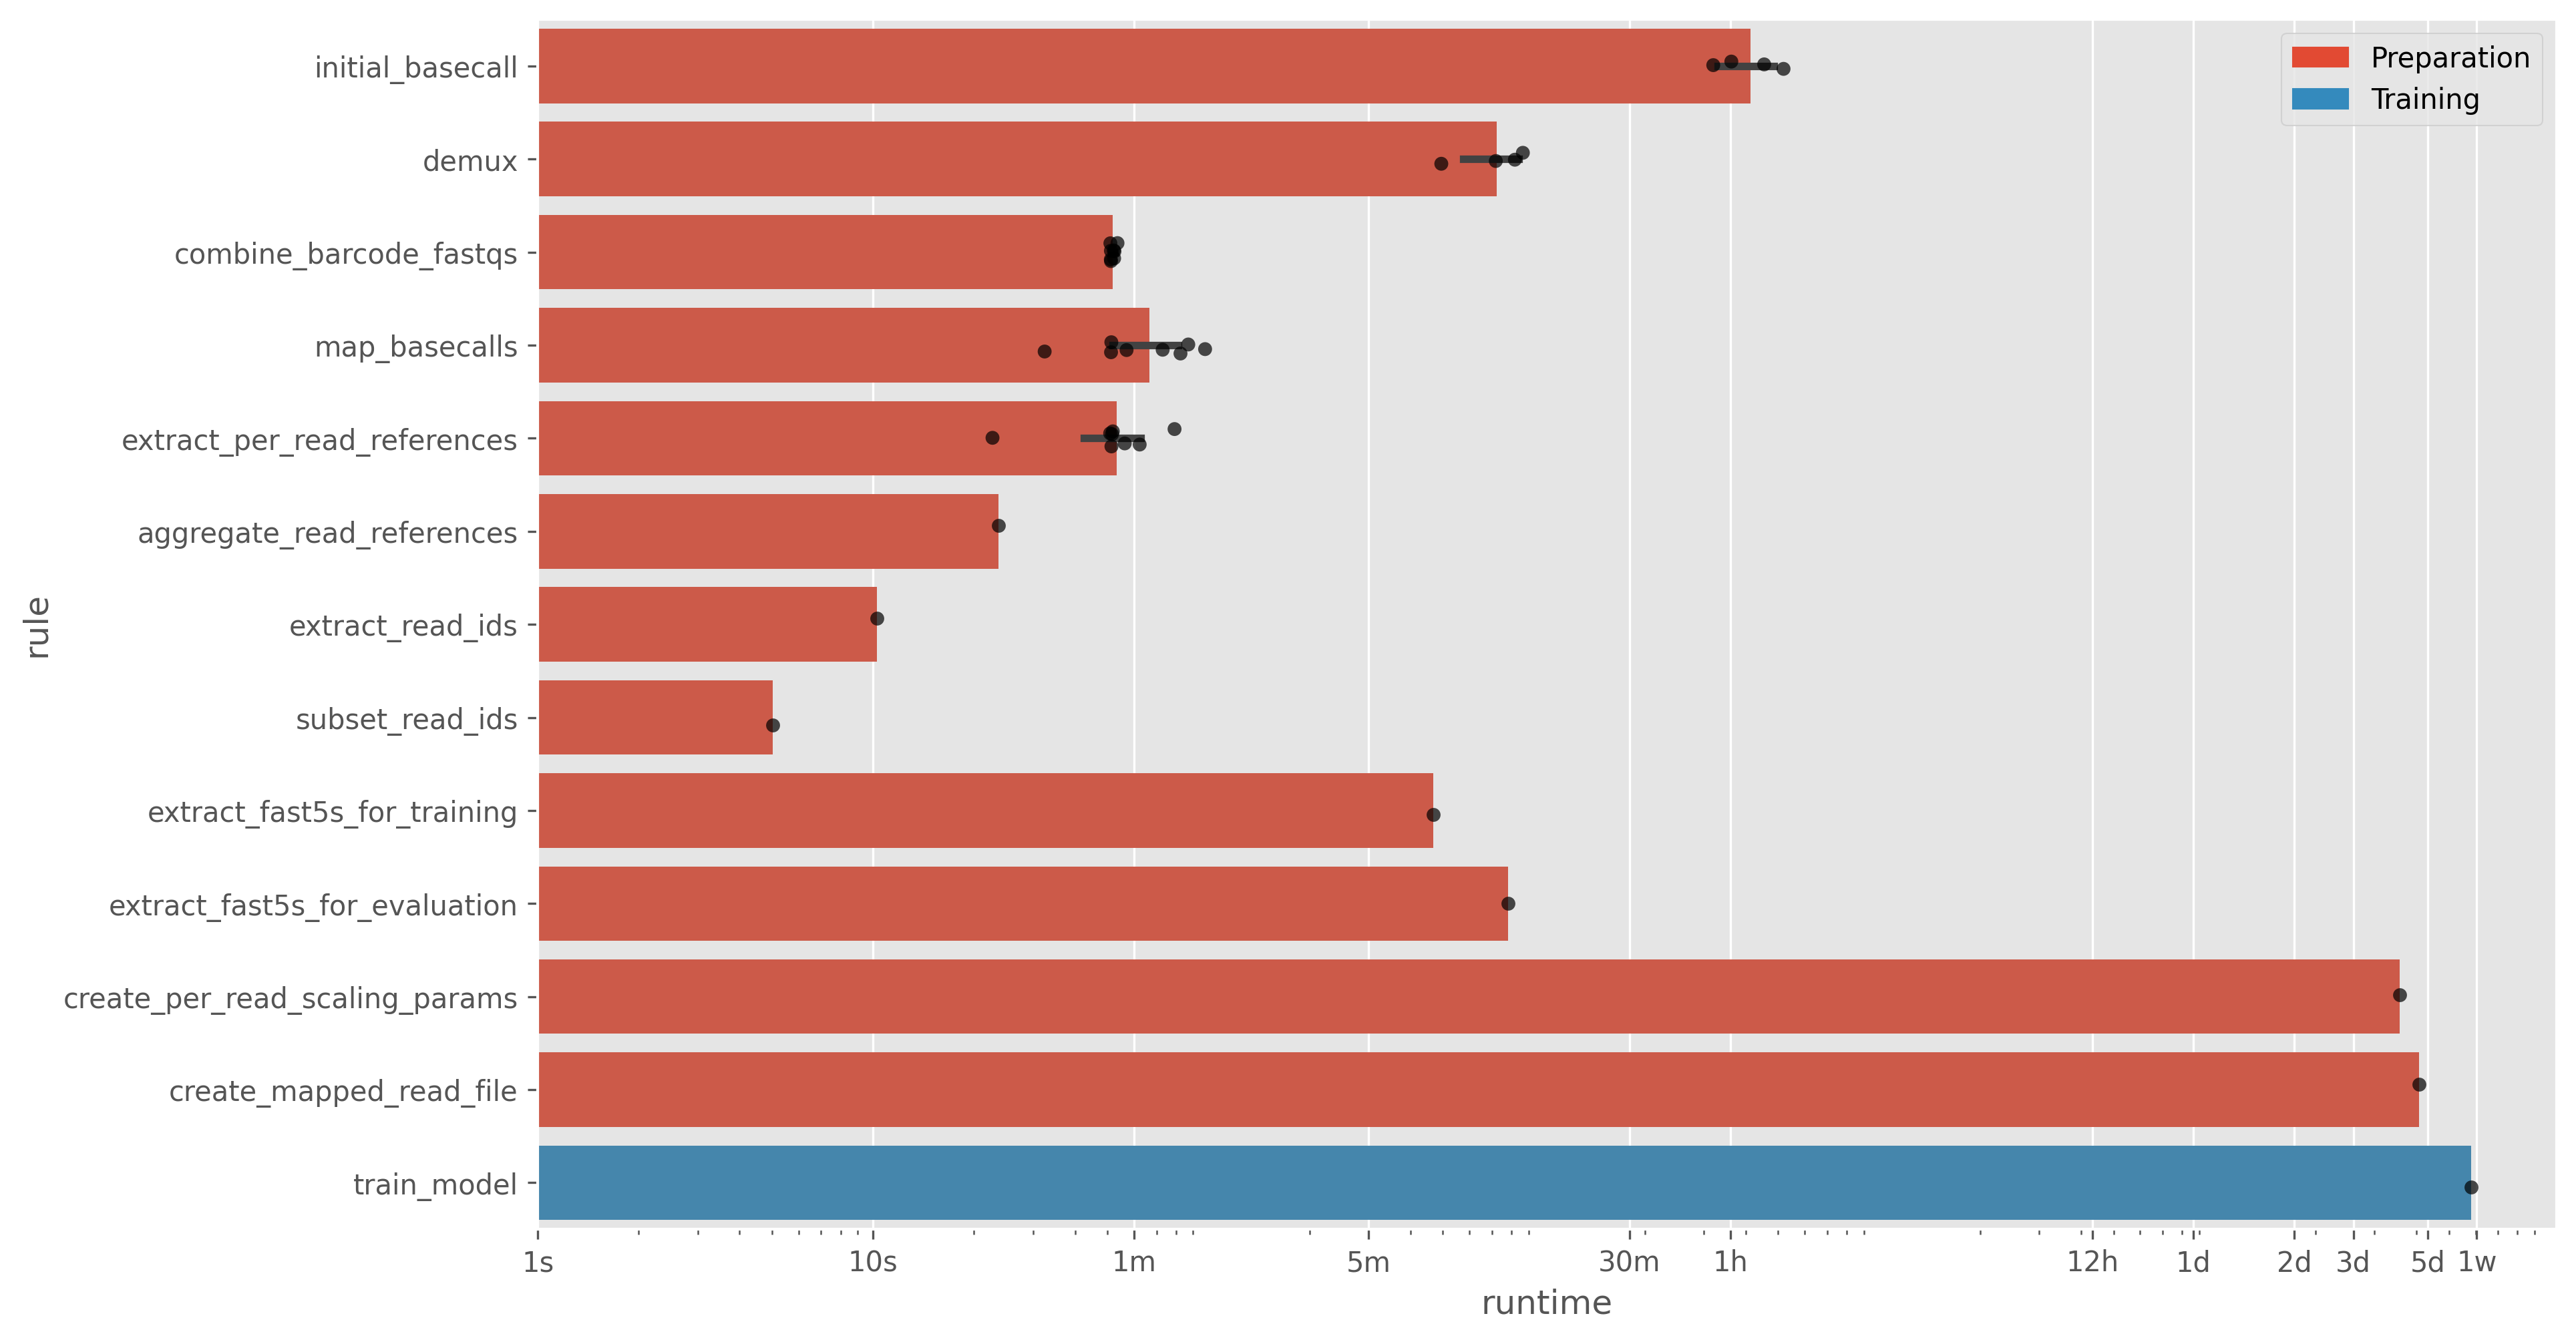
\includegraphics[width=0.9\textwidth]{Chapter4/Figs/prep_runtime.png}
\centering
\caption{Runtimes (x-axis) of the different stages (rules; y-axis) of preparing data for basecall model training. Each individual run is represented with a black point and rules that have multiple runs have black 95\% confidence interval bars. s=seconds; m=minutes; h=hours; d=days.}
\label{fig:prep_runtime}
\end{figure}

\autoref{fig:prep_runtime} shows the runtime of each step in the preparation phase of training. The two longest stages, trimming the raw signal (\vrb{create\_per\_read\_scaling\_params}) and mapping the raw signal to read-references (\vrb{create\_mapped\_read\_file}), took 4.1 and 4.7 days respectively. In total, the full preparation pipeline ran in 8.9 days. 

\subsubsection{Training}

The signal-to-sequencing mapping file produced from the preparation pipeline is the data file used for model training. In addition, we provide an initial model file from which training begins; the mLstm flipflop model distributed with \taiyaki{}.

We train the model using \taiyaki{}'s \vrb{train\_flipflop.py} script with the following parameters: a base layer size of 256; a model stride of 2; a window length over the data of 19; a minimum and maximum length of random training data chunks of 2000 and 4000, respectively; and a maximum learning rate of $0.002\sqrt{g}$, where $g$ is the number of GPUs used for training. The training took 162 hours (6.75 days) to complete on 2 GPUs and had a peak memory usage of 57GB. 

The final output from training the model is a checkpoint file, which we then convert to a \guppy{}-compatible JSON configuration file using \taiyaki{}.

%%%%%%%%%%%%%%%%%%%%%%%%%%%%%%%%%%%%%%%%%%%%%%%%%%%%%%%%%%%%%%%%%%%%%%%%%%%%%%%%%
\section{Evaluating a custom \ont{} basecalling model}

The model-training process produces a JSON file that can be used as a model configuration to basecall \ont{} reads using \guppy{}. The first step in evaluating whether our \mtb{}-specific model, \tubby{}, provides improved accuracy compared to \guppy{}'s default model is to basecall the validation reads that were set aside prior to training. These validation reads provide an unbiased dataset to evaluate on as they were not involved in the training process. Our evaluation process closely mirrors that of Wick \etal{} who produced the first taxon-specific \ont{} basecalling model \cite{wick2019}.  

We evaluate the read- and consensus-level accuracy of reads produced by \guppy{} and \tubby{} and assess the types of errors made by each. 

% =====
\subsection{Read-level performance}

The first evaluation metric, read BLAST identity, determines the read-level accuracy produced by the basecalling model. We align the basecalled reads to their respective truth assembly with \vrb{minimap2}, discarding secondary alignments (but keeping unmapped reads). From the resulting pairwise alignment (PAF) file we calculate the BLAST identity as, for each mapping, the number of matching bases divided by the length of the alignment. 

\autoref{fig:read-blast} shows the distribution of read BLAST identity values for each \guppy{} version and associated \tubby{} model. For all versions, \tubby{} has the highest read BLAST identity values - i.e., distribution of values is tighter, and the mode is further to the right. Interestingly, the best performing version for both models was 3.6.0, with a median BLAST identity of 95.54\% and 94.13\% for \tubby{} and \guppy{} respectively. \autoref{tab:read-blast} describes the summary statistics of the read BLAST identity distributions.

While version 3.6.0 has the highest median values for both models, it is important not to rely on this alone. For instance, version 4.4.0 has the highest minimum value for both models, and the highest mode (\tubby{} version 3.6.0 and 4.4.0 have the same mode). However, the percentiles are highest for version 3.6.0.

\begin{figure}
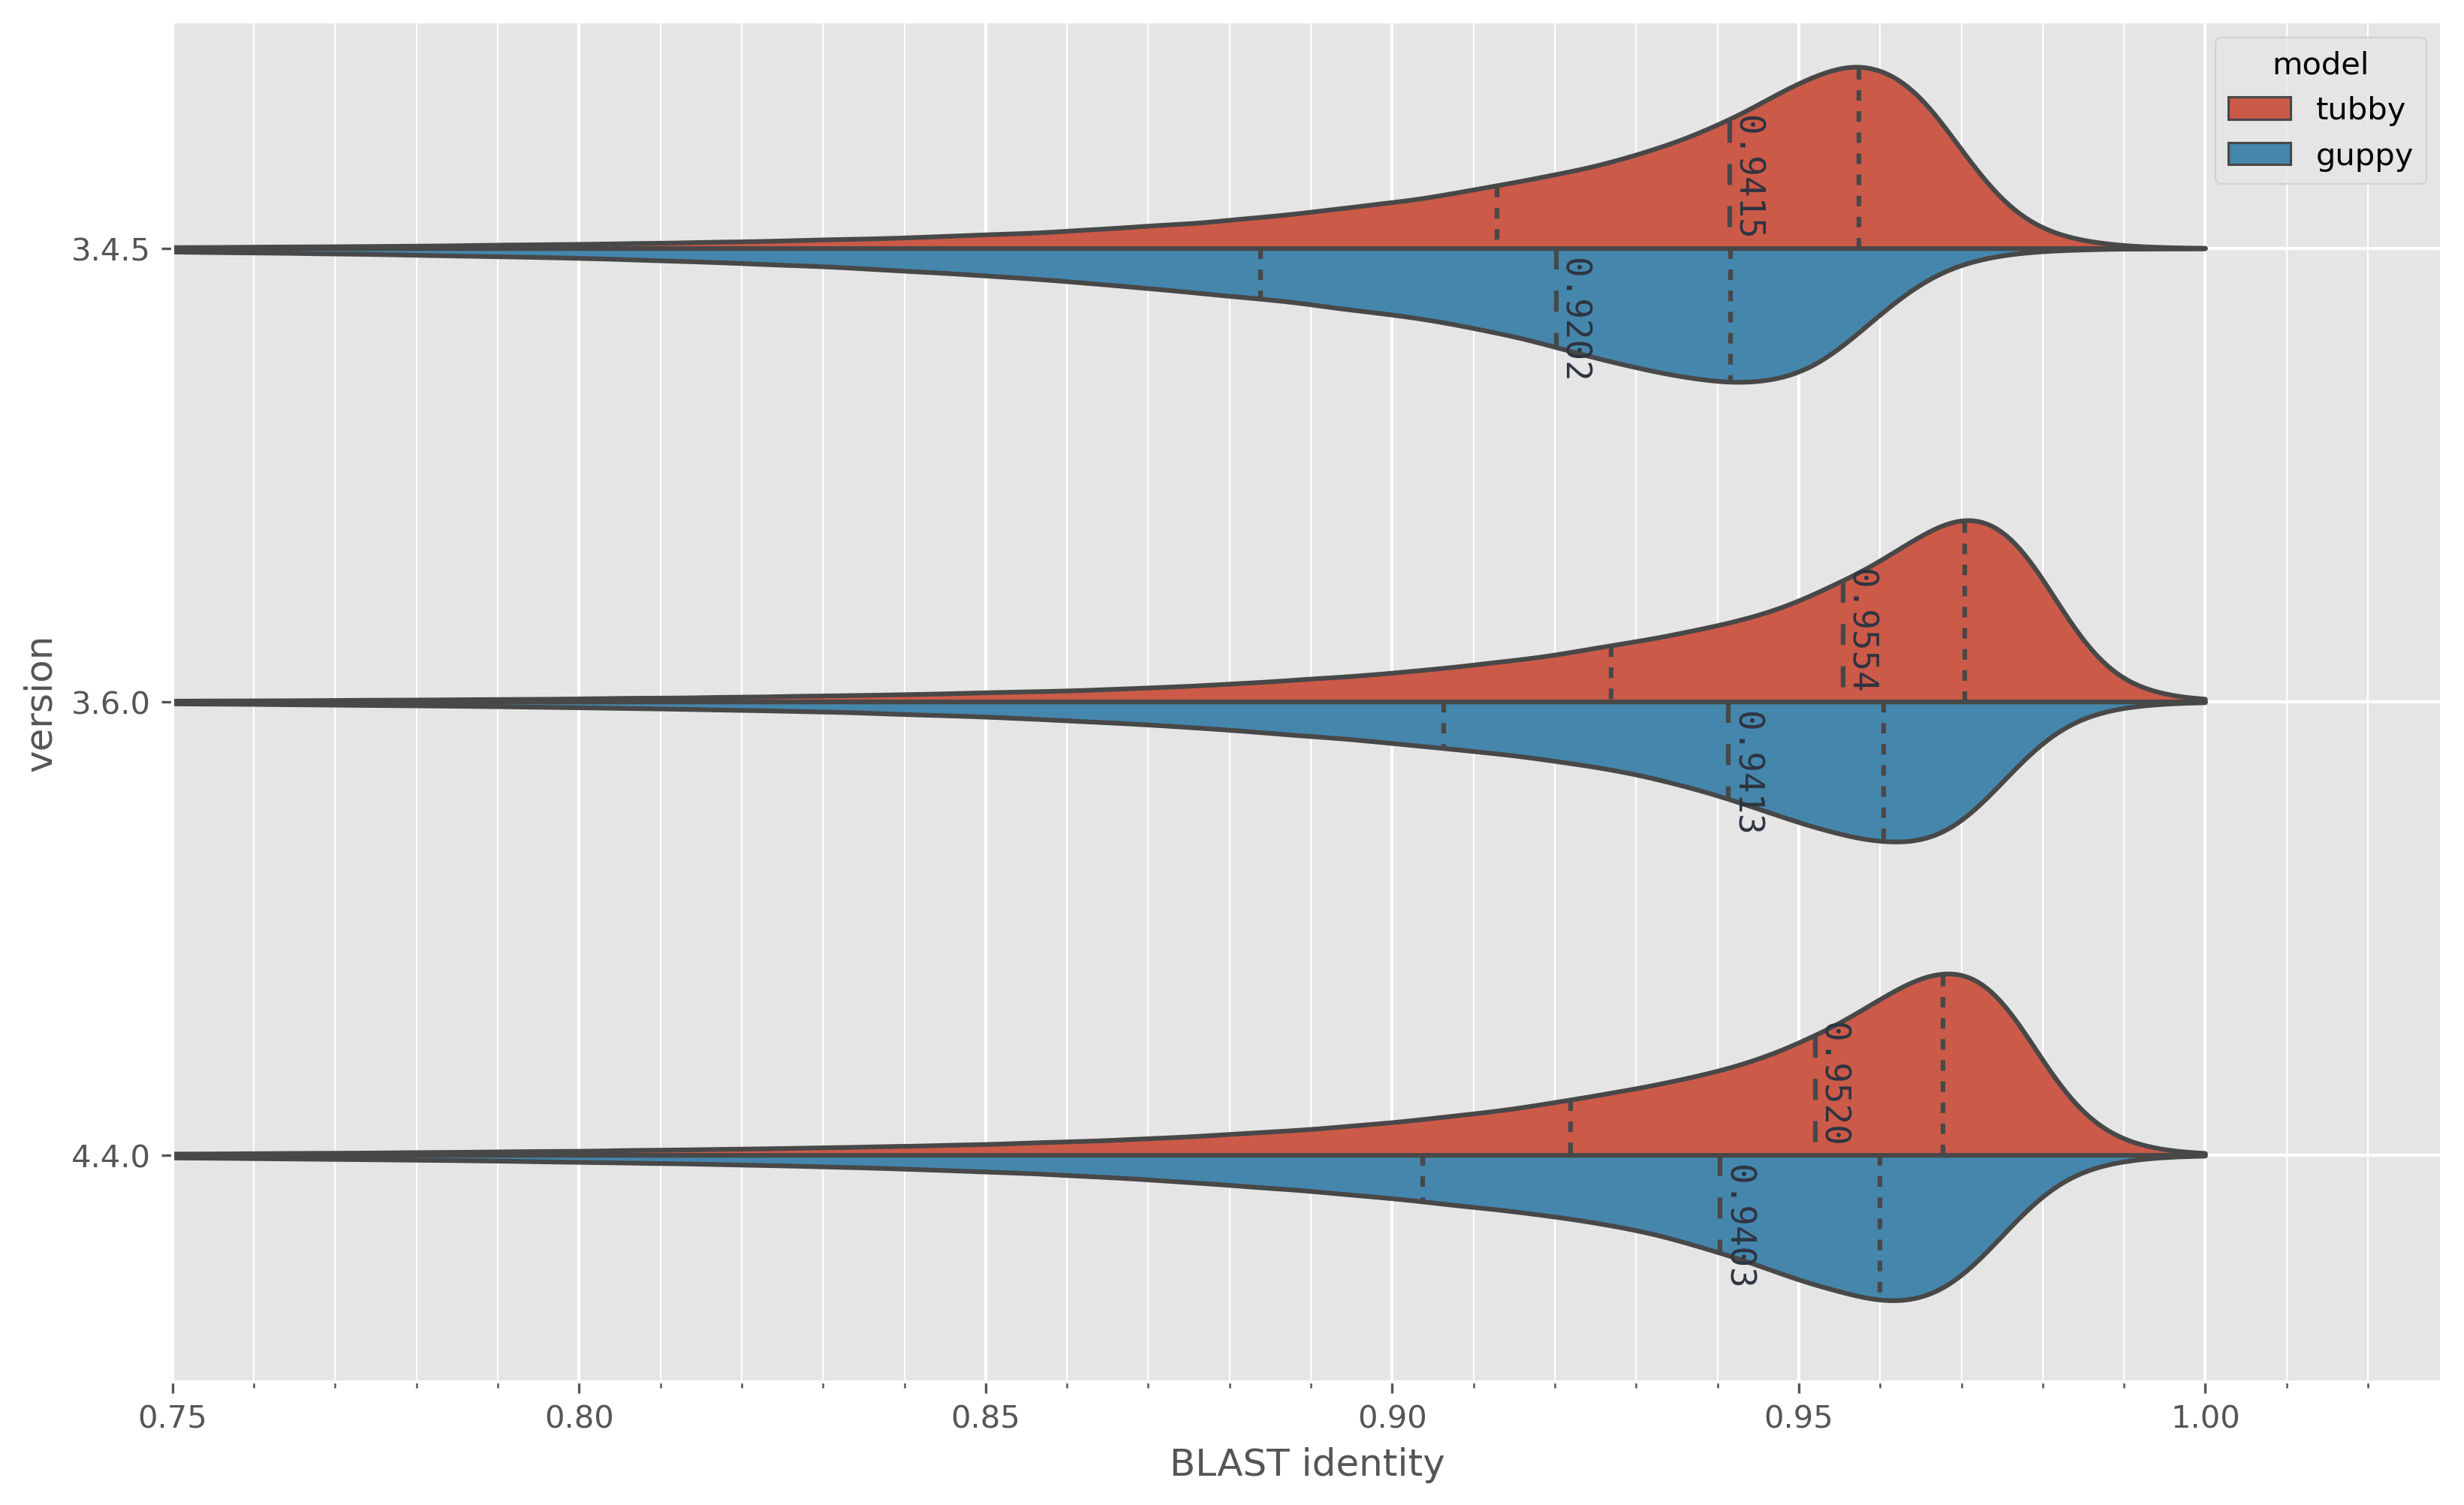
\includegraphics[width=0.9\textwidth]{Chapter4/Figs/read_blast_identity.png}
\centering
\caption{Read BLAST identity (x-axis) for the \mtb{}-specific basecalling model \tubby{} (red) compared with the default \guppy{} model (blue). Version (y-axis) indicates the \guppy{} version used for the basecalling prior to, and after, training. BLAST identity is the number of matching bases (in a read alignment) divided by the length of the alignment. The median value for each violin is annotated on the middle dashed line.}
\label{fig:read-blast}
\end{figure}

\begin{table}
\centering
\resizebox{\textwidth}{!}{%
\begin{tabular}{@{}llrrrrrrrrr@{}}
\toprule
Version                & Model & Count   & Mean   & std    & Min    & 25\%   & 50\%   & 75\%   & Max    & Mode    \\ \midrule
\multirow{2}{*}{3.4.5} & \guppy{} & 1047829 & 0.9067 & 0.0480 & 0.4186 & 0.8838 & 0.9202 & 0.9416 & 1.0000 & 0.9444 \\
                       & \tubby{} & 1047508 & 0.9295 & \textbf{0.0402} & 0.4619 & 0.9129 & 0.9415 & 0.9574 & 1.0000 & 0.9545 \\
\multirow{2}{*}{3.6.0} & \guppy{} & 1110664 & 0.9268 & 0.0474 & 0.4186 & 0.9063 & 0.9413 & 0.9604 & 1.0000 & 0.9615 \\
                       & \tubby{} & 1110098 & \textbf{0.9423} & 0.0413 & 0.4297 & \textbf{0.9269} & \textbf{0.9554} & \textbf{0.9704} & 1.0000 & \textbf{0.9688} \\
\multirow{2}{*}{4.4.0} & \guppy{} & 1144426 & 0.9247 & 0.0496 & \textbf{0.4751} & 0.9038 & 0.9403 & 0.9600 & 1.0000 & 0.9628 \\
                       & \tubby{} & 1143410 & 0.9381 & 0.0435 & 0.4723 & 0.9220 & 0.9520 & 0.9678 & 1.0000 & \textbf{0.9688} \\ \cmidrule(l){2-11} 
\end{tabular}%
}
\caption{Read BLAST identity summary statistics for the \mtb{}-specific basecalling model \tubby{} compared with the default \guppy{} model. Version indicates the \guppy{} version used for the basecalling prior to, and after, training. BLAST identity is the number of matching bases (in a read alignment) divided by the length of the alignment. Count refers to the number of reads evaluated. std=standard deviation.}
\label{tab:read-blast}
\end{table}

In addition to read BLAST identity, we also assess the relative read lengths produced by each basecalling model. We define relative read length as the length of the aligned part of the read, divided by the total length of the read. The purpose of this metric is to see whether there is a bias towards insertions (greater than 1.0) or deletions (less than 1.0). 

\autoref{fig:read-rel-len} shows that \tubby{} has a slight tendency towards deletions (shorter reads) compared to \guppy{}. However, this result is a little more complex than just looking at median values. The distribution of lengths for \guppy{} extends much further past 1.0 compared with \tubby{}, indicating an increase in insertions. We will return to this result when we look at the error types (\autoref{sec:tubby-error-types}). Summary statistics for the relative read lengths are shown in \autoref{tab:read-rel-len}.

\begin{figure}
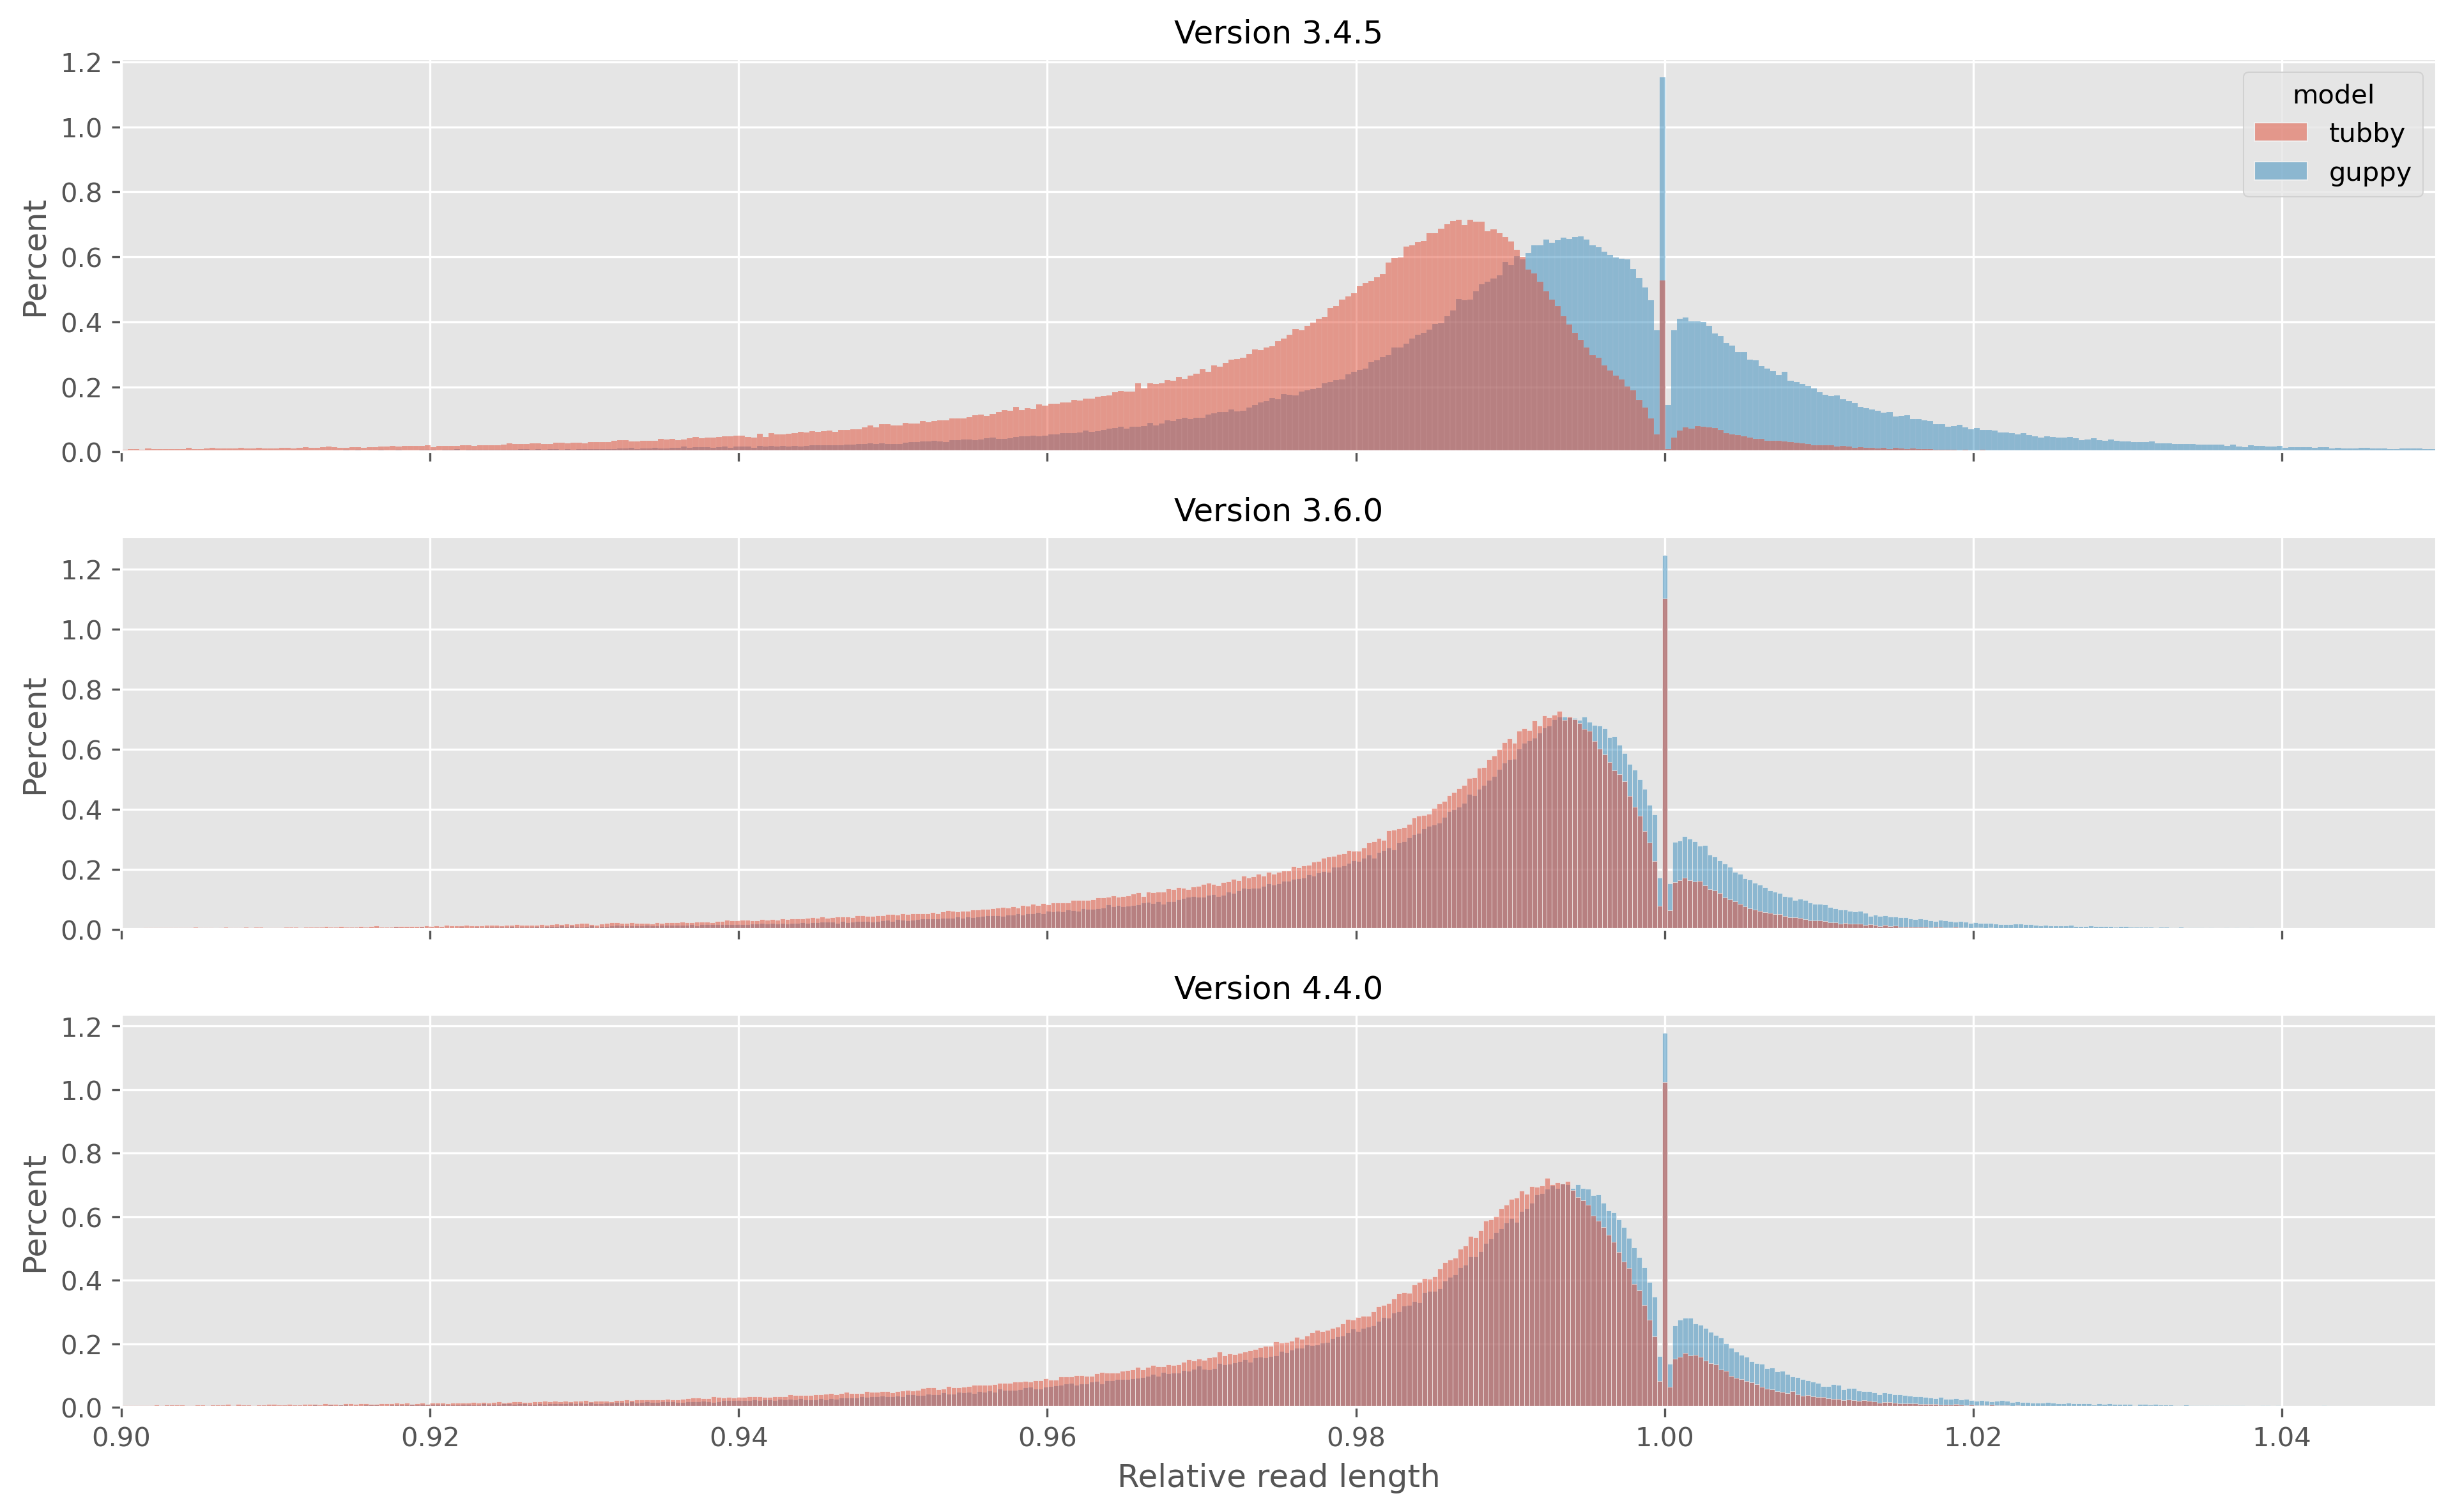
\includegraphics[width=0.9\textwidth]{Chapter4/Figs/read_rel_len.png}
\centering
\caption{Relative read length (y-axis) for the \mtb{}-specific basecalling model \tubby{} (red) compared with the default \guppy{} model (blue). Relative read length is the length of the aligned part of the read, divided by the total length of the read. Version indicates the \guppy{} version used for the basecalling prior to, and after, training.}
\label{fig:read-rel-len}
\end{figure}

\begin{table}
\centering
\resizebox{\textwidth}{!}{%
\begin{tabular}{@{}llrrrrrrrr@{}}
\toprule
Version                & Model & Count   & Mean   & std    & Min    & 25\%   & 50\%   & 75\%   & Max    \\ \midrule
\multirow{2}{*}{3.4.5} & \guppy{} & 1047829 & 0.9919 & 0.0240 & 0.4558 & 0.9842 & 0.9932 & 1.0014 & 1.9881 \\
                       & \tubby{} & 1047508 & 0.9764 & 0.0239 & 0.4936 & 0.9698 & 0.9822 & 0.9892 & 1.8949 \\
\multirow{2}{*}{3.6.0} & \guppy{} & 1110664 & 0.9873 & 0.0233 & 0.4495 & 0.9819 & 0.9914 & 0.9974 & 2.0322 \\
                       & \tubby{} & 1110098 & 0.9817 & 0.0241 & 0.4531 & 0.9761 & 0.9882 & 0.9943 & 1.9031 \\
\multirow{2}{*}{4.4.0} & \guppy{} & 1144426 & 0.9862 & 0.0241 & 0.5085 & 0.9806 & 0.9907 & 0.9969 & 1.9146 \\
                       & \tubby{} & 1143410 & 0.9814 & 0.0246 & 0.4963 & 0.9758 & 0.9879 & 0.9941 & 1.8851 \\ \cmidrule(l){2-10} 
\end{tabular}%
}
\caption{Relative read length (y-axis) for the \mtb{}-specific basecalling model \tubby{} (red) compared with the default \guppy{} model (blue). Relative read length is the length of the aligned part of the read, divided by the total length of the read. Version indicates the \guppy{} version used for the basecalling prior to, and after, training. Count refers to the number of reads evaluated. std=standard deviation.}
\label{tab:read-rel-len}
\end{table}

% =====
\subsection{Consensus-level performance}
\label{sec:tubby-error-types}

To assess consensus-level accuracy, we first need to produce assemblies for each model's generated reads. To allow for comparison of these model-specific consensus sequences to the truth assembly, a reference-guided method is needed to ensure overall structure of the truth and consensus sequences is the same. We use `rebaler`(CITE), a tool developed for specifically this use-case. Briefly, `rebaler` aligns the reads to a reference sequence and replaces that sequence with the sequence from the best alignments, producing an unpolished assembly. After this, it polishes the assembly with `racon` to produce a consensus sequence. We then calculate the consensus accuracy by following a similar approach used for the read accuracy. However, as we have a single sequence, we cut the consensus into 10kbp chunks and treat these chunks as reads. These chunks are mapped to the reference/truth and the consensus accuracy is reported as the BLAST identity of the alignments produced.  

To assess consensus accuracy the basecalled reads were assembled using `rebaler`. `rebaler` was developed by Wick *et al.* for the purposes of evaluating basecalling models and is a reference-guided assembly approach (see \todo{link to relevant methods section}). Here we show consensus accuracy in a similar manner to read identity. Each "read" in this context is the result of chopping the `rebaler` assembly of the reads up into 10kbp "chunks" to simulate reads. These chunks are then mapped back to the original assembly and we use BLAST identity as the measure of accuracy. \autoref{fig:combined_basecall}B shows tubby has higher consensus accuracy (median 0.9993) compared with \guppy{} (median 0.9992). The consensus accuracy improvement of 0.0001 equates to approximately 440 less erroneous positions in the \mtb{} assembly.
% \begin{figure}
% 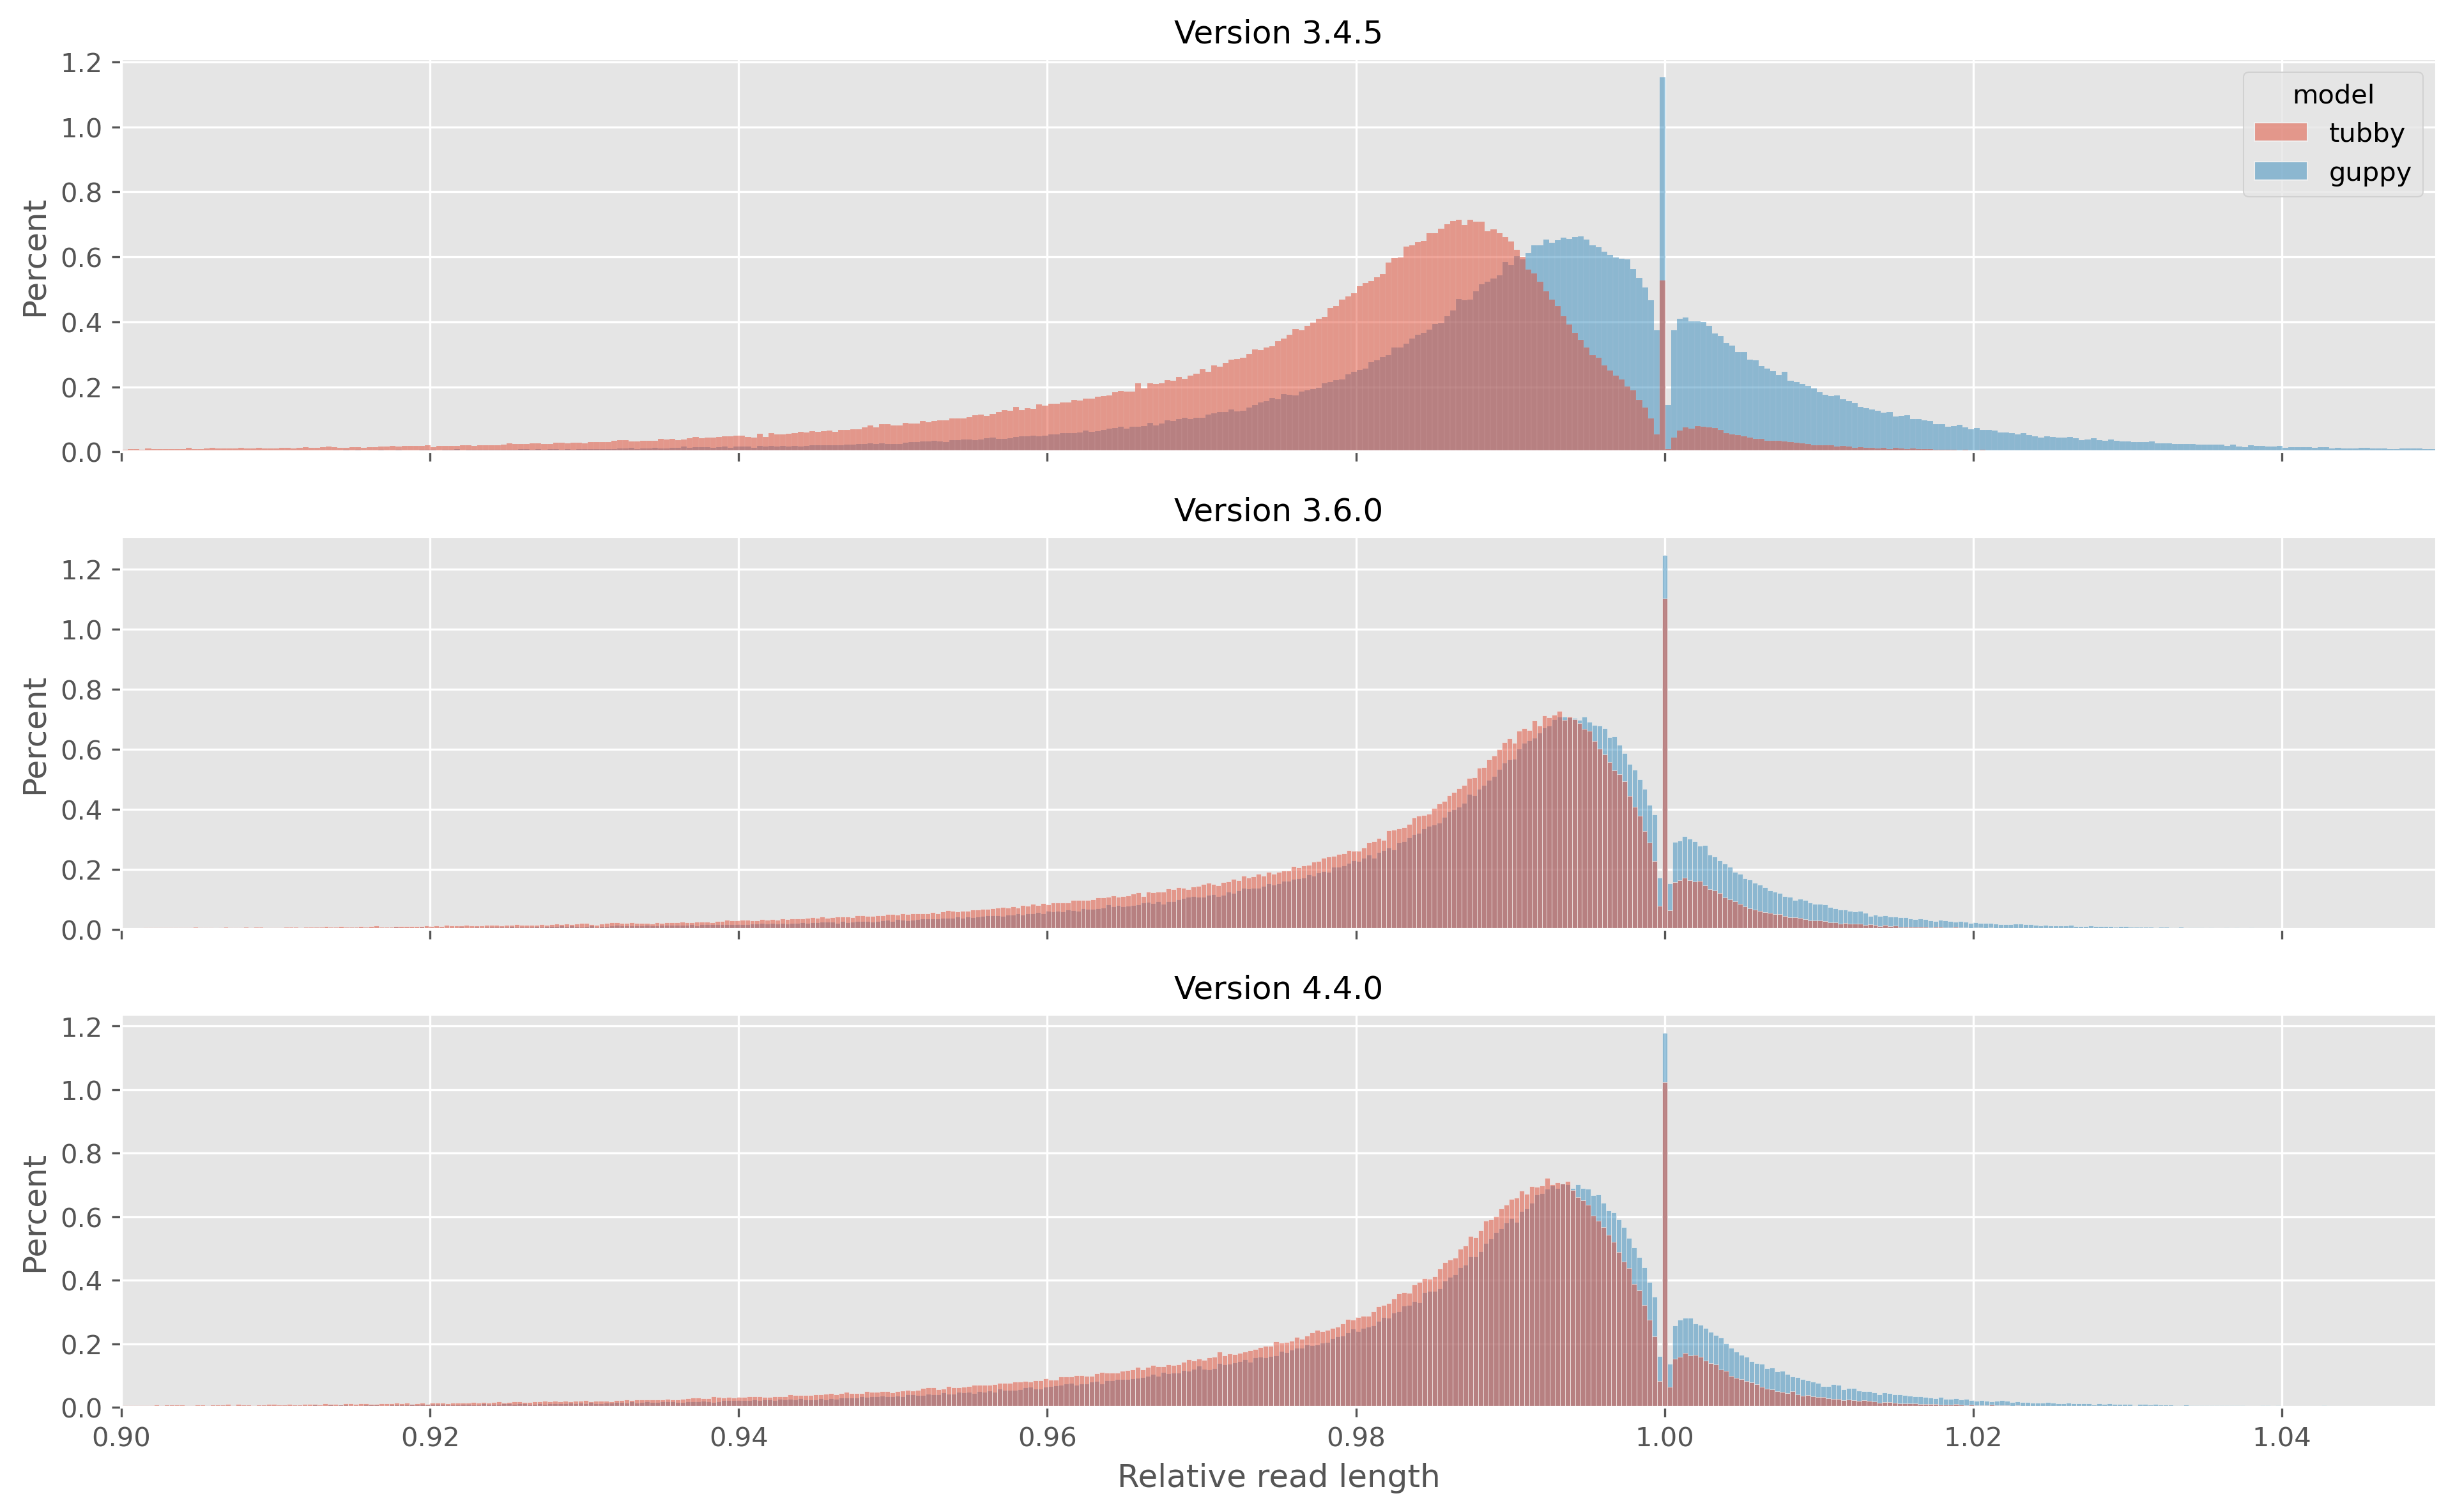
\includegraphics[width=0.9\textwidth]{Chapter4/Figs/read_rel_len.png}
% \centering
% \caption{A) Read BLAST identity (Y-axis) for the \mtb{}-specific basecalling model 'tubby' (blue) compared with the default \guppy{} model (red). BLAST identity is the number of matching bases (in a read alignment) divided by the length of the alignment. B) Consensus BLAST identity (Y-axis), where consensus refers to "chunks" of the genome assembly produced by the basecalled reads, for each model, mapped to the truth genome. C) Relative read length (Y-axis) for the two models. Relative read length is the length of the aligned part of the read, divided by the total length of the read. D) Consensus relative length. Relative length is the length of the aligned part of the consensus "chunk", divided by the total length of the "chunk". Note: the Y-axes have all been zoomed-in to allow closer inspection of the majority of data.}
% \label{fig:read-rel-len}
% \end{figure}
% ====
\subsection{Error types}

Lastly, we classify the the types of errors that occur in the assemblies produced from each model's output. The `rebaler` assembly for each model and sample combination was aligned to the sample's truth assembly using `nucmer`(CITE). `nucmer` produces all positions of difference - errors in this case - between the two sequences. We classify errors as Dcm if the reported difference occurs in a known 5-methylcystosine methyltransferases motif(CITE), homopolymer insertion or deletion if the difference involves as base being added/removed from a region containing 3 or more of that same base. All deletions, insertions, and substitutions that do not fit into one of these categories after reported in their own group.

Here we classify the types of errors that occur in the `rebaler` assemblies and look at how these errors compare across models. To determine the errors, we categorise the differences between the truth and `rebaler` assemblies (see \todo{link to relevant methods}). \autoref{fig:error_types} shows that the greater part of the error types (for both models) are attributable to deletions, with most being homopolymer deletions. We do however see that, except for non-homopolymer deletions, tubby's errors are lower than \guppy{}'s \todo{add some concrete numbers}. In the case of both insertion types, tubby has approximately 3.5-fold less insertions than \guppy{} - although these constitute a small portion of the overall errors. Both models have a very low level of Dcm-methylation errors, which is a nice control of sorts as \mtb{} does not have any known 5-methylcystosine methyltransferases(CITE)\improvement{ensure the wording of this and correct and that the claim is also correct}.

% \begin{figure}
% 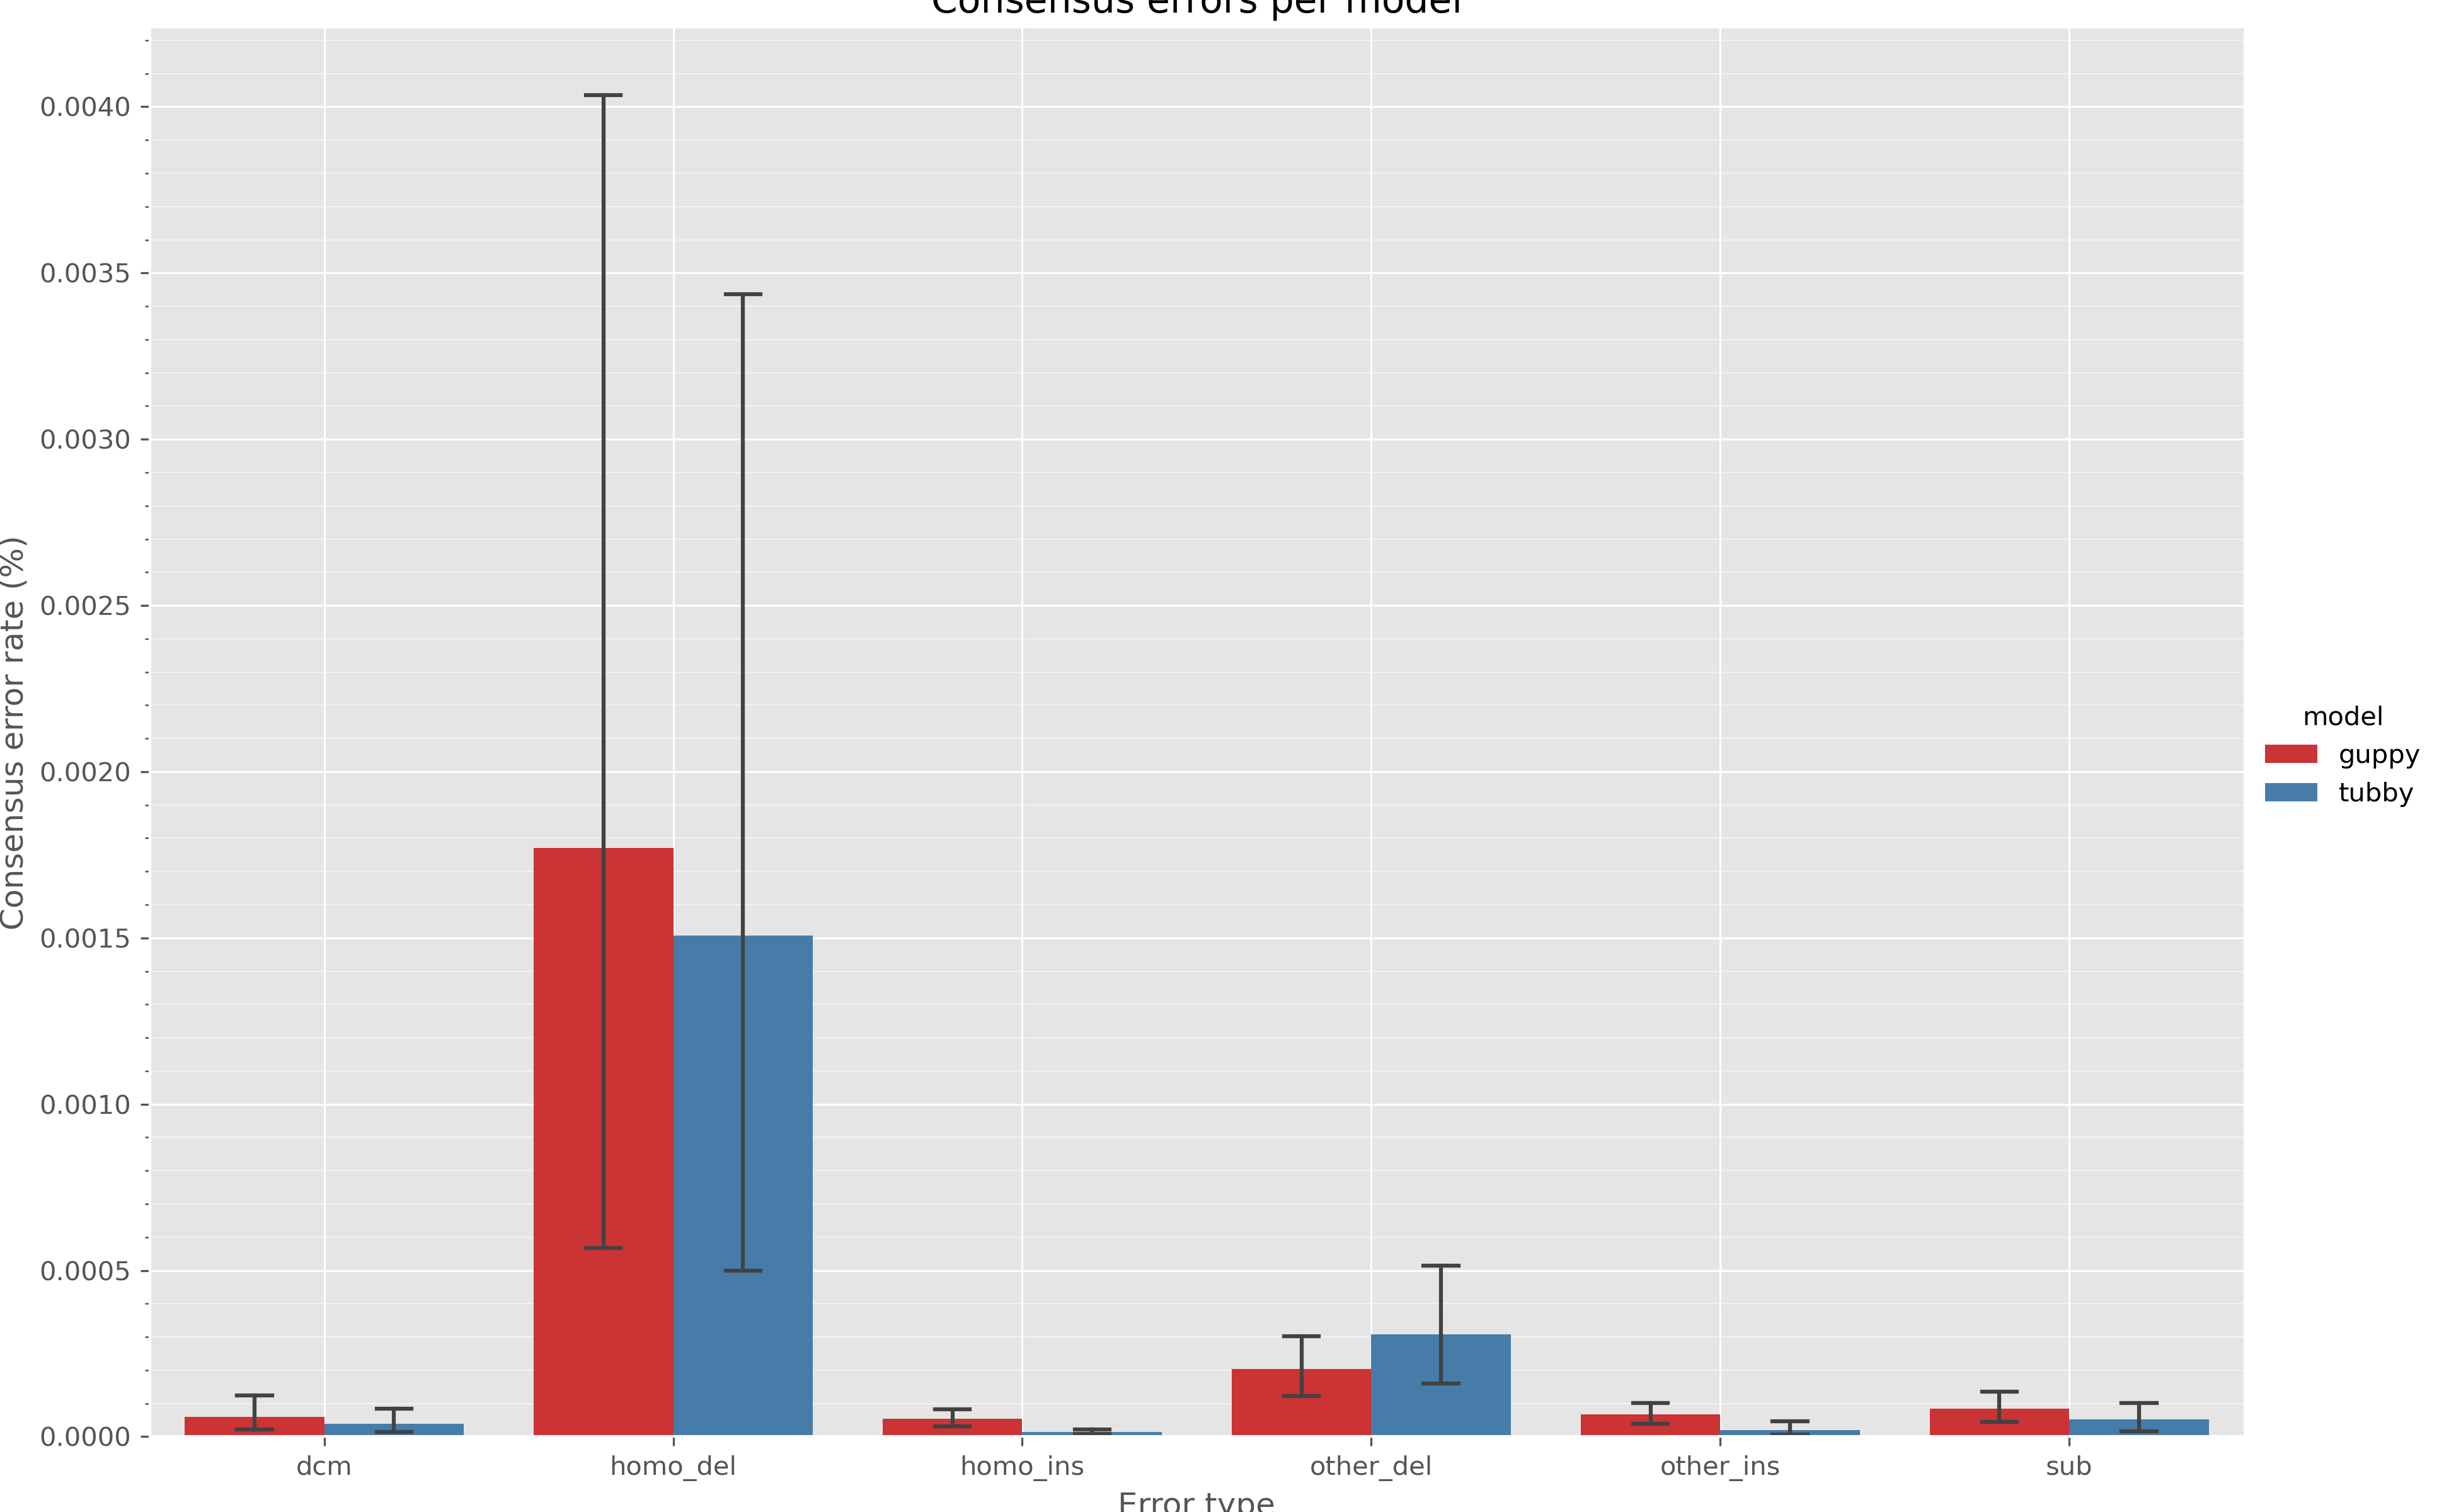
\includegraphics[width=1.0\textwidth]{Chapter4/Figs/consensus-error-types.png}
% \centering
% \caption{Error types in the `rebaler` assemblies produced from reads basecalled with tubby (blue) and \guppy{} (red). The consensus error rate is the percentage of the assembly these errors compose. The errors are per-assembly, so the confidence intervals represent variation in error types between samples/assemblies. dcm refers to Dcm-methylation motifs. homo\_ins/del are homopolymer insertions or deletions. sub is single-base substitutions.}
% \label{fig:error_types}
% \end{figure}

%%%%%%%%%%%%%%%%%%%%%%%%%%%%%%%%%%%%%%%%%%%%%%%%%%%%%%%%%%%%%%%%%%%%%%%%%%%%%%%%%
\section{Discussion}

%%%%%%%%%%%%%%%%%%%%%%%%%%%%%%%%%%%%%%%%%%%%%%%%%%%%%%%%%%%%%%%%%%%%%%%%%%%%%%%%%
\section{Conclusion}

%%%%%%%%%%%%%%%%%%%%%%%%%%%%%%%%%%%%%%%%%%%%%%%%%%%%%%%%%%%%%%%%%%%%%%%%%%%%%%%%%
\section{Future work}

%%%%%%%%%%%%%%%%%%%%%%%%%%%%%%%%%%%%%%%%%%%%%%%%%%%%%%%%%%%%%%%%%%%%%%%%%%%%%%%%%
\section{Availability of data and materials}
%%!TEX root = ../thesis.tex
%*******************************************************************************
%******************************   Fifth Chapter   ***************************
%*******************************************************************************
\chapter*{Conclusion}
\addcontentsline{toc}{chapter}{Conclusion} \markboth{Conclusion}{}
\label{chap:conclusion}
%%%%%%%%%%%%%%%%%%%%%%%%%%%%%%%%%%%%%%%%%%%%%%%%%%%%%%%%%%%%%%%%%%%%%%%%%%%%%%%%%

This thesis shows that genome graphs and Nanopore sequencing can be combined to provide valuable insight into genomic variation within bacteria. In particular, we have demonstrated how these two techniques can be combined to improve public health applications for M. tuberculosis.

We began this work by describing a method for novel variation discovery in bacterial genome graphs with Pandora (Chapter 2). We then showcased how Pandora's genome graph approach improves variant recall (Illumina and Nanopore) and precision (Nanopore) compared to traditional linear genome methods.

Chapter 3 demonstrated that, for M. tuberculosis, Nanopore sequencing data produces SNP calls of equal precision to Illumina, with a slight decrease in recall. We then established that Nanopore SNP calls from BCFtools lead to putative transmission clusters consistent with those from Illumina. That is, Nanopore-based clusters do not miss any samples from clustering - no false negatives - and have a small number of (false positive) additional clustered samples. While Pandora was able to provide clusters with no false negatives, the rate of false positives was much higher than BCFtools. However, we outlined some avenues for future work to improve this poor false positive performance, including a different approach to constructing the loci reference graphs. 

In Chapter 4, we established the concordance of antimicrobial resistance predictions between Illumina and Nanopore sequencing data with the tool Mykrobe. Predictions from the two technologies were consistent, except for isoniazid, where we found a high false-positive rate in Nanopore data - driven by systematic indel errors. In addition, we implemented a new software program, DRPRG, which uses Pandora to predict drug resistance. DPRG predictions were consistent with Mykrobe for both sequencing technologies, albeit with a slight increase in the false-negative rate for isoniazid. Most importantly, DRPRG can identify off-catalogue mutations and return unknown predictions for the relevant drug(s). These novel mutations are precise and reduce the number of missed resistance calls.

Finally, we trained a species-specific Nanopore basecalling model that produces more accurate M. tuberculosis reads and assemblies than the default model. This improvement in accuracy coincides with a decrease in homopolymer insertions and deletions - two known systematic issues with Nanopore data.

% In this case we are not going to ask for any changes other than to add a concluding discussion section. This should address the wider implications of the methods and technologies described in the thesis, not only in the context of current practice but also the potential for new approaches based on an understanding of the biology and genetics of TB and drug resistance. We would like you to take a step back from the focus on current monitoring and clinical methodologies, and discuss how the deeper aims of the field might be advanced using the technologies and computational approaches your work is based on.
% You have 3 months to complete this, but we expect that it should take much less than that - a few pages is what we have in mind. Hopefully it should be a useful exercise to go through in terms of where you see your research going in future.

% scaling pandora up to thousands of genomes

% PanRGs that extend beyond the concept of species - metaPanRGs?

% investigating pe/ppe genes with genome graphs. improve our knowledge of host-pathogen interactions, virulence, and other unknown functions/relationships - AMR?

% mixtures, along with resistance calls in these mixtures

% real-time analysis of mtb samples on the ground. Go beyond the theory and have direct from sputum DST in remote areas - i.e., Madagascar drone stuff?  Novel variants help determine which samples need to be sent back to the reference lab and which can be started on treatment immediately. Clustering could also help identify where further empidemiological investigation is warranted for superspreaders etc. How does flongle feed into this - The  release  of  the  Flongle  adapter  in  2019  provides  a  low-output 327sequencing solution(2 Gb) at 90 USD per Flongle flow cell, which is the lowestset-328up cost of any sequencing platform currently available. Read-until can be used for articifical sample/region depletion/enrichment

% epigenetic modifications have  been  associated  with  drug  resistance,  virulence,and regulation  of gene 69expression  profiles - Phelan  J,  de  Sessions  PF,  Tientcheu  L,  Perdigao  J,  MachadoD,  Hasan  R,  Hasan  Z, 422Bergval  IL,  Anthony  R,  McNerney  R,  Antonio  M,  Portugal  I,  Viveiros  M,  Campino  S, 423Hibberd  ML,  Clark  TG.2018.  Methylation  in  Mycobacterium  tuberculosis  is  lineage 424specific with associated mutations present globally. Sci Rep 8:160.4255.Gomez-Gonzalez  PJ,  Andreu  N,  Phelan  JE,  de  Sessions  PF,  Glynn  JR,  Crampin  AC, 426Campino  S,  Butcher  PD,  Hibberd  ML,  Clark  TG.2019.  An  integrated  whole  genome 427analysis of Mycobacterium tuberculosis reveals insights into relationship between its 428genome, transcriptome and methylome. Sci Rep 9:520

% https://journals.asm.org/doi/epdf/10.1128/JCM.00646-21 Nanopore/Mtb review from Anzaan

% expanding drprg to predict new and repurposed drugs   


\noindent
The methods and technologies described in this thesis have the potential to advance existing approaches and enable new ones. 

In the context of bacterial genomics in general, pan-genome reference graphs, as used by Pandora, will eventually facilitate the simultaneous analysis of thousands to tens-of-thousands samples. Such population-scale analyses will open the door for a multitude of novel insights into the bacterial pan-genome. Some of these future applications include fine-grained analysis of the accessory genome at scale. Being able to investigate the accessory genome at this scale, with resolution Pandora enables, will allow for 

\todo[inline]{What new insights will population-scale accessory pan-genome analysis allow?}

Genome-wide association studies (GWAS) are another application that will benefit from such pan-genome graph methods. GWAS has traditionally been difficult to perform in bacteria due to XXX (reference variability?). Current GWAS approaches, termed pan-GWAS only correlate accessory genes to phenotypic traits. However, we foresee Pandora enabling the correlation of individual variants to traits - a dramatic improvement in scale. 

\todo[inline]{Are there bacterial GWAS methods that already do SNP-GWAS?}
\todo[inline]{How/will pandora allow SNP-scale GWAS? What is it that enables this?}
\todo[inline]{Maha has some TB GWAS papers - check these out}

Looking even further ahead, the pan-genomic model we have described in this thesis - where we let go of gene ordering - lends itself to allowing for the relaxation if species requirements. An ongoing question within microbiology is that of what defines a species? We know that many bacterial species share common genes, and can even share genes. Indeed, many metagenomic applications disregard species definitions and focus purely on loci. In an environmental context, one may only care about the presence or absence of particular loci such as AMR genes, or even unique genes the indicate the presence of microbes of interest. Pandora can even go one step further and provide resolution within these loci of interest. An example of this could be that species A and B have gene X, but the sequence of gene X differs slightly been the two - say one SNP. 

\todo[inline]{Check out some recent Eduardo Rocha papers on the bacterial species question}
\todo[inline]{Look up some environmental applications which only care about loci - not species}
\todo[inline]{Read up on TB mixed inference}

While not a current ability of Pandora, we believe that it will be possible to use Pandora to determine the abundance of different paths in a reference graph. This capability will allow inference of mixed samples. Not only would this be useful in the environmental example just outlined, but also in clinical applications. Multiple infections are known to happen in TB. This can become quite insidious when a minor clone has resistance to a drug, or drugs, that the major clone is susceptible to. If a patient is put on a regimen without the knowledge of the minor clone, it is likely that the minor clone will sweep to dominance, placing the patient back at the beginning of treatment.

\todo[inline]{discuss how nanopore feeds into aiding mixed inference as long reads capture longer range haplotype information}


%\include{Chapter6/chapter6}
%\include{Chapter7/chapter7}



% ********************************** Back Matter *******************************
% Backmatter should be commented out, if you are using appendices after References
%\backmatter

% ********************************** Bibliography ******************************
\begin{spacing}{0.9}

% To use the conventional natbib style referencing
% Bibliography style previews: http://nodonn.tipido.net/bibstyle.php
% Reference styles: http://sites.stat.psu.edu/~surajit/present/bib.htm

\bibliographystyle{apalike}
%\bibliographystyle{unsrt} % Use for unsorted references  
%\bibliographystyle{plainnat} % use this to have URLs listed in References
\cleardoublepage
\bibliography{References/references} % Path to your References.bib file


% If you would like to use BibLaTeX for your references, pass `custombib' as
% an option in the document class. The location of 'reference.bib' should be
% specified in the preamble.tex file in the custombib section.
% Comment out the lines related to natbib above and uncomment the following line.

%\printbibliography[heading=bibintoc, title={References}]


\end{spacing}

% ********************************** Appendices ********************************

\begin{appendices} % Using appendices environment for more functunality

% %!TEX root = ../thesis.tex
% ******************************* Thesis Appendix A ****************************
\chapter{Supporting work for Chapter 3}

% ===========================================================

\section{DNA sequencing methods}

\subsection{Illumina}

\towrite[inline]{once i get this info from collabs}

\subsection{\ont{}}

\towrite[inline]{once i get this info from collabs}

\subsection{PacBio}
\label{app:pacbio-seq}

35 of the Malagasy samples were sequenced and processed at the Next Generation Genomics Core within Cold Spring Harbor Laboratory. Samples were quantified with a Qubit dsDNA HS Assay Kit and QC’d through a Pulsed Field Gel Electrophoresis system. Then, samples were sheared at 10kb using a Megaruptor device and size-selected to 8-10 kb with a Blue pippin instrument - followed by 0.45X ampure bead purification. The PacBio library protocol SMRTbell Express Template Prep Kit 2.0 was used for each sample. Briefly, the first step was the removal of single-stranded overhangs followed by DNA Damage Repair, End-Repair/A-tailing, Ligation of overhang barcoded adaptors and sample pooling. A total of 3 pools were produced: LID50532 (16 samples), LID50533 (10 samples), and LID50534 (9 samples). After pooling, 0.5X ampure bead clean up was performed. A Sequel I instrument was used to sequence the 3 library pools. Libraries were annealed for an hour and bounded for an hour using sequel binding kit 3.0. Bound SMRTbell complexes were then purified with ampure beads. The run was set up as 10kb length for 10 hours movie time. The Sequel 1M V2 SMRT cells were used for each library.  

The circular consensus was called via the SMRTlink graphical user interface version 6.0.0.47841.

% ===========================================================

\section{Benchmark of long read genome assembly methods for \mtb{}}
\label{app:asm}
Samples with greater than 30x coverage across all three sequencing technologies were chosen to produce high-quality assemblies. In total, this left us with 9 Malagasy samples. There has been many new genome assembly methods produced since the last known assessment of \mtb{} long-read assemblies \cite{bainomugisa2018}. As such, we compare five assemblers and select the one that produces the most consistently good results. The reason for this comparison is that different assembly algorithms can produce quite varied results depending on sequencing technology used, species, or computational resource availability(CITE).  

The assembly tools we assess are Canu, Flye, Unicycler, HASLR, and Spades(CITE \& VERSION). HASLR and Unicycler are hybrid assemblers that take Illumina reads along with one long-read file, although Unicycler does not require both. Spades is also a hybrid assembler but takes an arbitrary number of different sequencing technologies. Canu and Flye are both long-read-only assemblers.

The first step in the assembly pipeline is the trimming of adapter sequences in the Illumina reads using Trimmomatic(CITE). Two assemblies were then produced for each sample - one for each long-read technology. The exception to this was Spades, for which there is just one assembly for each sample, as it accepts all reads simultaneously. 

Canu, in some cases, produces assembly bubbles, which are regions where it believes there is a heterozygous locus due to differences in haplotypes. While it is not impossible some samples could be multi-clonal, we chose to remove bubbles from the Canu assemblies, effectively choosing the dominant haplotype for downstream analysis.  

All contigs in the resulting assemblies were species-classified using Centrifuge(CITE). We remove any contigs whose classification places them outside of the Mycobacterium Tuberculosis Complex. Polishing of these decontaminated assemblies is done in two steps; first using long-reads and Racon(CITE) with default settings, followed by short reads with Pilon(CITE). Default Pilon settings were used for \ont{} assemblies, but for PacBio we don't correct for SNPs. PacBio CCS reads are already a consensus from multiple reads, so allowing Illumina reads to fix at a per-base level lead to decreased per-base accuracy (results not shown).  

We annotate both the polished and unpolished genome assemblies using Prokka(CITE). We assess relative correctness of all assembly variations for a given sample using Assembly Likelihood Estimator (ALE)(CITE). Assembly statistics were generated for each sample using Quast(CITE) with the \mtb{} reference genome, H37Rv (accession: NC\_000962.3), as a reference. We do not expect our assemblies to be the same as H37Rv, but it can provide insights into the structural completeness and genome size. Lastly, we assess per-base accuracy using a custom script. As input for the script, we provide a BAM file of the Illumina reads mapped to the assembly and the pileup generated by the Samtools subroutine \vrb{mpileup}(CITE). We require a quorum of 90, which is the percentage of reads that must agree with the assembly at each position, and a minimum depth of 10x. Any position within the assembly that does not meet both of these conditions is considered a disagreement. The output from the script is a collection of statistics and a BED file containing all disagreement positions.

Assessing the quality of \denovo{} assemblies is non-trivial and requires aggregation of various metrics. Whilst a reference genome exists for \mtb{} (H37Rv), there are enough differences between the \mtb{} lineages that using this reference would not be appropriate for our purposes. We will look at each assessment metric individually, and then decide on the best assembly method from this information.

\subsection{Assembly Likelihood Evaluation score}

The assembly likelihood evaluation (ALE) score is a reference-free metric that describes the likelihood of an assembly given its \kmer{} distribution, and the likelihood of the reads being generated from that assembly. It combines information such as read quality, agreement in the alignment of reads to assembly, mate-pair orientation, paired-end read length, and depth of sequencing. Importantly, the ALE score can be used to compare assemblies of the same genome, which is exactly the use case we have. Whilst ALE scores are not insightful on their own, the difference \textit{between} assembly scores gives the relative probability of correctness. So for each sample, we are interested in the assembly that has the \textit{highest} ALE score.  

Across the 9 samples, \vrb{flye} has the highest ALE score in five cases, whilst \vrb{spades} was the most probable assembly in two, with \vrb{unicycler} and \vrb{canu} having the maximum score in one sample each (\autoref{fig:ale_score}). Note, this is considering both polished and unpolished assemblies together for each tool. When considering which long-read sequencing technology produces the greatest ALE score, CCS had the top score in 7/9 samples. In 6/9 samples, the highest ALE score was from a polished assembly.

\begin{figure}
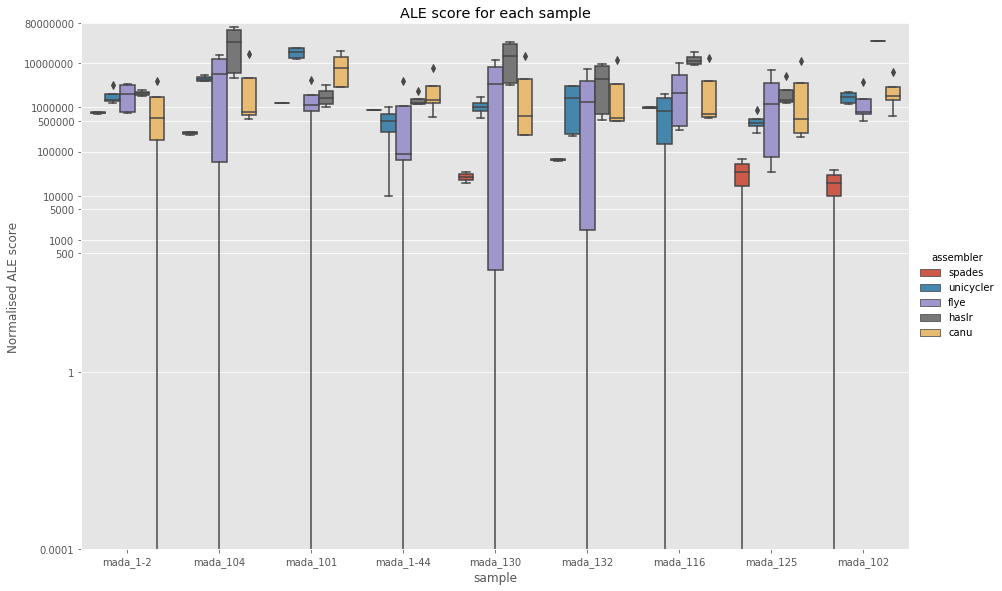
\includegraphics[width=1.0\textwidth]{Appendix1/Figs/ale_score.png}
\centering
\caption{The normalised assembly likelihood evaluation (ALE) score (Y-axis) for each sample (X-axis), coloured by assembly tools. ALE score is a metric describing the likelihood of an assembly. The normalisation is done by subtracting the assembly's score from the maximum (best) score for that sample, giving a relative probability of correctness. Each box represents different technologies and polishing status for each assembler.}
\label{fig:ale_score}
\end{figure}

\subsection{Disagreement rate}
\label{app:asm_disagree}

The disagreement rate is an approximation of the per-base accuracy of the assembly. We map Illumina reads to the assembly and calculate what proportion of positions do 90\% of the reads agree with the assembly nucleotide.  

In 7/9 samples, a \vrb{HASLR} assembly had the lowest disagreement rate, followed by \vrb{unicycler} having the minimum in 2/9. Polished genomes produced the lowest disagreement rate in 8/9 samples and \ont{}-based assemblies had the best accuracy in 6/9 samples. While it isn't so surprising that assemblies polished with Illumina reads have a lower disagreement rate, it is unexpected that \ont{} would produce more accurate assemblies (\autoref{fig:disagree_rate}). One caveat to keep in mind here - and this is the reason for looking at many different metrics - is that there is an element of overfitting to this metric: we assess using Illumina, and so naturally, assemblies polished with Illumina produce better results. That is not to say this statistic is void, but that it should be used with caution.

\begin{figure}
\includegraphics[width=1.0\textwidth]{Appendix1/Figs/disagree_rate.png}
\centering
\caption{The disagreement rate (Y-axis) for each assembler (X-axis), coloured by the sequencing technology. Disagreement rate is the percentage of sites in the assembly where Illumina reads do not have at least 90\% quorum. Each box/point represents different samples and polished status for the relevant assembler/technology combination.}
\label{fig:disagree_rate}
\end{figure}

As part of calculating the disagreement rate, we also produced a BED file listing all positions with less than 90\% agreement. This BED file can be used as a genome mask when using the assembly for later analysis.

\subsection{Number of contigs}

As \mtb{} has only a single, circular chromosome, for an assembly to be structurally complete, there should only be a single contig in the final assembly. However, it is not always appropriate for an assembly method to produce a single contig as data quality, depth of sequencing, read length, and/or repetitive content of the genome can hamper this goal(CITE). Conversely, receiving a single contig as output is no guarantee of its quality for similar reasons to the previous, multi-contig scenario. For the purposes of this benchmark, considering on conjunction with the other metrics, the number of contigs can be a useful datum for selecting our favoured assembly. If an assembly has a single contig, and scores well on other metrics, we would be more inclined to choose it over another assembly with similar metrics, but many more contigs.

Across all combinations of assembly conditions, \vrb{spades} (8/18), \vrb{flye} (18/32) and \vrb{canu} (16/32) produced far more single-contig assemblies than the hybrid methods (\autoref{fig:num_contigs}). \vrb{unicycler} produced no single-contig genomes, whilst \vrb{HASLR} yielded only 2/32. When considering sequencing technology, PacBio (26/72) had many more single-contig assemblies than \ont{} (10/72). Note, \vrb{spades} assemblies use all three technologies and are not considered in the technology single-contig totals.

\begin{figure}
\includegraphics[width=1.0\textwidth]{Appendix1/Figs/num_contigs.png}
\centering
\caption{The number of contigs (Y-axis) produced from each assembly (X-axis), coloured by sequencing technology. Each box/point represents different samples and polished status for the relevant assembler-technology combination.}
\label{fig:num_contigs}
\end{figure}

\subsection{Length of assembly}

As mentioned earlier, comparing the assemblies to the \mtb{} reference genome (H37Rv) is not appropriate, however, it's length/size can be used as an aid for selection. The size of any lineage's genome is not expected to differ from the reference by more than \texttildelow 30 kilobases \cite{kato2001}. Considering the genome size in addition to disagreement rate is particularly informative. It would be quite easy for an assembly method to produce very accurate per-base contigs by refusing to produce sequence for "harder" parts of the genome. While such an assembly would score well on disagreement rate, it would not do so well when considering how close to the expected genome size it is. The length of the assembly also clearly shows when a method is outputting \textit{too much} sequence.

When comparing the size of each assembly to that of H37Rv, we found a fairly even spread across assemblers for the closest size to H37Rv. For 3/9 samples, \vrb{canu} has the smallest size difference, followed by \vrb{spades} (2/9), \vrb{unicycler} (2/9), \vrb{HASLR} (1/9) and \vrb{flye} (1/9). An honourable mention should be made of \vrb{flye} and \vrb{spades} as they had much lower variation in size compared to the other approaches. In terms of sequencing technology, in 6/9 samples CCS produced the genome size closest to H37Rv. Polished assemblies had the closer size in 5/9 samples.

\begin{figure}
\includegraphics[width=1.0\textwidth]{Appendix1/Figs/asm_len.png}
\centering
\caption{Size/length (Y-axis; in base-pairs (bp)) of each assembly (X-axis), coloured by each sequencing technology. The horizontal dashed line represents the size of the \mtb{} reference genome (4,411,532bp). Each box/point represents different samples and polished status for the relevant assembler-technology combination. Note: the Y-axis has been limited to allow for greater resolution of similarity to the H37Rv size}
\label{fig:asm_len}
\end{figure}

\subsection{Contamination detection}

The decontamination step in the assembly pipeline revealed that one sample, \vrb{mada\_1-2}, contained contigs from three different species: \textit{Mycobacterium intracellulare}, \textit{Dermacoccus nishinomiyaensis}, and \mtb{}. These contigs were all at sufficient coverage to not be considered background noise. For the assembly assessment analysis only the contigs from \mtb{} were used, but figures for the assessment metrics in the previous sections show this sample is an outlier in almost all metrics. Given this profuse contamination, \vrb{mada\_1-2} will not be used in any analysis where these assemblies are used for truth validation purposes.

\subsection{Summary}

In conclusion, considering all assessment metrics, \vrb{flye} and \vrb{spades} assemblies were consistently the better performing methods across all of the criteria outlined in this section. As most of the validation analyses that these assemblies will be used for involve comparing Illumina and \ont{} data to a "neutral truth", the unpolished PacBio CCS assemblies from \vrb{flye} were selected for use. The differences between the polished and unpolished CCS assemblies was almost negligible and do not outweigh the benefit of having a single-technology PacBio assembly that can be used as an unbiased reference point for comparing the other two technologies.

% ===========================================================

\section{Masking of the \mtb{} reference graph}
\label{app:mask}

We investigated three different strategies for masking the positions that go into the \mtb{} reference graph in \autoref{sec:tbprg}. The first of these was not to use a mask at all and apply all variants that passed all other filters in the \cryptic{} VCF. Compared to the final solution we chose - removing loci with 30\% or more positions in the mask - this lead to the sparse \prg{} MSA step having a peak memory usage of 357GB (1.7 times more than \autoref{tab:build-prg}) and a wall clock time of 13.5 hours (compared to 1.25). The dense \prg{} MSA step likewise saw higher memory usage (370GB) and wall clock time (44.6 hours). In addition, when updating these \prg{}s to include novel variants (\autoref{sec:pandora-filters}), the MSA stage took on the order of days to complete. 
The second masking strategy was just to remove the VCF positions that occur within the H37Rv genome mask mentioned in \autoref{sec:tbprg}. This approach would ensure there would be sequence covering the whole H37Rv genome within the reference graph. This approach yields construction times similar to those in \autoref{tab:build-prg}. However, this caused the novel variant discovery stage of \pandora{} to hit the 7 day compute node run limit for some samples. The cause of this huge increase can be explained by the fact that the positions within the mask are, by definition, repetitive (low complexity). As such, we \pandora{} initiates \denovo{} variant discovery in these sections of the genome, the path enumeration step outlined in \autoref{sec:path-enum} gets caught in cycles within the de Bruijn graph - a limitation outlined in \autoref{sec:denovo-limits}.
The third strategy is the one we ended up using - removing loci with 30\% or more positions in the mask. The 30\% figure was settled on as it provided a good balance between losing sections of the H37Rv genome (see \autoref{fig:loci-mask}) and providing acceptable computational performance for all steps in the reference graph construction and \pandora{} variant-calling pipeline.

\begin{figure}
     \centering
     \begin{subfigure}[b]{0.475\textwidth}
         \centering
         \includegraphics[width=\textwidth]{Appendix1/Figs/loci-lost.png}
         \caption{}
         \label{fig:loci-lost}
     \end{subfigure}
     \hfill
     \begin{subfigure}[b]{0.475\textwidth}
         \centering
         \includegraphics[width=\textwidth]{Appendix1/Figs/pos-lost.png}
         \caption{}
         \label{fig:pos-lost}
     \end{subfigure}
        \caption{\textbf{a)} Proportion of loci lost (y-axis) when removing those with a certain fraction (x-axis) of their positions within the genome mask. \textbf{b)} Proportion of total genome positions lost (y-axis) when removing loci with a certain fraction (x-axis) of their positions within the genome mask.}
        \label{fig:loci-mask}
\end{figure}

% ===========================================================

\section{Precision and recall of all variant calls from \pandora{}}
\label{app:pandora-all-vars}

Although we only use SNPs for identifying transmission clusters, we also assessed \pandora{} variant calls for all variants, including indels up to a length of 20bp, in \autoref{fig:pandora-filters-all} (\pandora{} SNPs are evaluated in \autoref{sec:map-var-calls}). We did this for the sake of future work that might be interested in using \pandora{} indel calls, such as predicting drug resistance. Again, the sparse \prg{} gave better precision and recall than the dense one. Using all variants, there was a recall improvement to 75.48\% (all filters) - up 3.49\% from SNPs only. Precision on the other hand sees a drop to 95.90\% when assessing all variants - compared to 100\% for SNPs only. Given the large drop in precision it is clear that \pandora{} indel-calling needs further improvement, however, indel calling (deletions especially) are a known limitation of \ont{} \cite{jain2018,wick2019}.

\begin{figure}
\begin{center}
\includegraphics[width=0.90\columnwidth]{Appendix1/Figs/pandora-precision-recall-filters-all-variants.png}
\caption{{Precision (bottom) and recall (top) of SNPs for COMPASS (purple) and all variants (maximum indel length of 20bp) for \pandora{} with sparse (red) and dense (blue) \prg{}s. The \pandora{} boxes start with no filters on the left, with each box moving to the right adding a filter to the previous box. The COMPASS box is a reference to the precision and recall of Illumina variant calls. Linear PRG density refers to the fact that COMPASS uses a single, linear reference genome as opposed to \pandora{}, which uses a genome graph. The black points refer to single data points for the seven samples used. MIN\_COV=minimum depth of coverage;MIN\_SB=minimum strand bias;MIN\_GT\_CONF=minimum genotype confidence score;MIN\_FRS=minimum fraction of read support.
{\label{fig:pandora-filters-all}}%
}}
\end{center}
\end{figure}

% ===========================================================

\section{An illustrated example of clustering similarity metrics}
\label{app:cluster-example}

\autoref{sec:cluster-similarity} outlines three metrics - SACR, SACP and XCR - for evaluating the similarity between two different strategies for transmission clustering. In order to provide the reader with greater intuition for the relevance of each metric, we present an illustrated example in \autoref{fig:cluster-example}. We take \autoref{fig:example-truth} to be the truth clusters and \autoref{fig:example-test} to be some test clusters. These are akin to Illumina and \ont{} clusters, respectively, in \autoref{sec:cluster-similarity}). The individual recall and precision values for each sample in \autoref{fig:example-truth} are shown in \autoref{tab:cluster-example}. SACR and SACP are \emph{sample-averaged}, so their values for this example are 0.82 and 0.83 respectively. To highlight the objective of SACR, we take the truth and test clusters containing the sample $F$. Samples $F$, $G$, $H$ and $I$ are shared between both, but $J$ is missing from the test cluster. To calculate the individual recall for $F$, we take the intersection size of the truth and test clusters it exists in and divide it by that size again, plus the number of samples in the truth cluster that are not in the test cluster - $\frac{4}{5}=0.8$. Ee do the same for the precision of sample $D$, expect we add the number of samples in the test cluster not in the truth cluster to the denominator - giving $\frac{2}{3}=0.66$. The relevance of the XCR metric is best exemplified by the test cluster containing samples $L$ and $M$. As we calculate SACR and SACP for all samples in the truth clusters, these two samples would be ignored. However, they are samples that - according to the truth - should not be part of any cluster. SACR and SACP cannot capture these extra clusterings if they do not contain clustered truth samples. XCR covers this limitation and is the proportion of non-clustered samples (singletons) in the truth that are clustered in the test (see \autoref{eq:xcr}). As \autoref{fig:cluster-example} does not show singletons, let us pretend there are 20 singletons in the truth (including samples $L$ and $M$). This would give an XCR of $2/20=0.1$.

\begin{figure}
     \centering
     \begin{subfigure}[b]{0.4\textwidth}
         \centering
         \includegraphics[width=\textwidth]{Appendix1/Figs/illumina-cluster-example.png}
         \caption{}
         \label{fig:example-truth}
     \end{subfigure}
     \hfill
     \begin{subfigure}[b]{0.4\textwidth}
         \centering
         \includegraphics[width=\textwidth]{Appendix1/Figs/ont-cluster-example.png}
         \caption{}
         \label{fig:example-test}
     \end{subfigure}
        \caption{Illustrative examples of transmission clustering. \textbf{a)} represents truth clusters, while \textbf{b)} is clustering from some "test" method we would like to compare to \textbf{a}. The nodes represent samples with the numbers on the edges connecting them indicating the distance between those two samples. The red nodes indicate samples with a clustering disparity between the two clusterings.}
        \label{fig:cluster-example}
\end{figure}

\begin{table}
\centering
\begin{tabular}{|c|c|c|}
sample & recall & precision \\
\hline
A      & 1.0    & 1.0       \\
B      & 1.0    & 1.0       \\
C      & 1.0    & 1.0       \\
D      & 1.0    & 0.66      \\
E      & 1.0    & 0.66      \\
F      & 0.8    & 1.0       \\
G      & 0.8    & 1.0       \\
H      & 0.8    & 1.0       \\
I      & 0.8    & 1.0       \\
J      & 0.0      & 0.0        
\end{tabular}
\caption{Cluster recall and precision results for each sample in \autoref{fig:cluster-example}}
\label{tab:cluster-example}
\end{table}

% ===========================================================

\section{Selecting \ont{} SNP thresholds to define transmission clusters}
\label{app:dist-sweep}

In \autoref{sec:snp-dist}, we found linear models that describe the relationship between the Illumina and \ont{} SNP distance between pairs of samples. Using the equations for each model, we can infer a \ont{} threshold corresponding to a given Illumina threshold. We investigate how well these model-based thresholds perform by using the cluster similarity metrics defined in \autoref{sec:cluster-similarity}. To assess the performance, we by looking at the SACR, SACP, and XCR for all threshold values surrounding the model-based threshold and seeing whether the model-based performs best.

\subsection{bcftools}

For the Illumina SNP thresholds 0, 2, 5, and 12, the corresponding bcftools model-inferred thresholds are 1, 3, 5, and 10 (red vertical dashed lines in \autoref{fig:bcftools-dist-sweep}). Based on the threshold sweep in \autoref{fig:bcftools-dist-sweep}, the best SNP distance thresholds to use for bcftools are deemed 0, 2, 5, and 11 as these provide the best balance between the three similarity metrics.

\begin{figure}
\begin{center}
\includegraphics[width=0.90\columnwidth]{Appendix1/Figs/bcftools-threshold-sweep.png}
\caption{{Illumina and \ont{} (bcftools) transmission cluster similarity for various SNP distance threshold. Each subplot compares the \ont{} clustering for the threshold on the x-axis to the Illumina clustering based on the distance (threshold) in the subplot title. SACR (red), SACP (blue), and $1-$XCR are represented by the lines with the band around the line indicating the 95\% confidence interval. The red, vertical, dashed lines indicate the model-based prediction of what the \ont{} SNP distance threshold should be based on the Illumina distance for that subplot.
{\label{fig:bcftools-dist-sweep}}%
}}
\end{center}
\end{figure}

\subsection{\pandora{} single-sample}

For the Illumina SNP thresholds 0, 2, 5, and 12, the corresponding \pandora{} single-sample model-inferred thresholds are 15, 17, 19, and 24 (red vertical dashed lines in \autoref{fig:map-dist-sweep}). Based on the threshold sweep in \autoref{fig:map-dist-sweep}, the best SNP distance thresholds to use for \pandora{} single-sample are deemed 16, 18, 18, and 27 as these provide the best balance between the three similarity metrics.

\begin{figure}
\begin{center}
\includegraphics[width=0.90\columnwidth]{Appendix1/Figs/map-threshold-sweep.png}
\caption{{Illumina and \ont{} (\pandora{} single-sample) transmission cluster similarity for various SNP distance threshold. Each subplot compares the \ont{} clustering for the threshold on the x-axis to the Illumina clustering based on the distance (threshold) in the subplot title. SACR (red), SACP (blue), and $1-$XCR are represented by the lines with the band around the line indicating the 95\% confidence interval. The red, vertical, dashed lines indicate the model-based prediction of what the \ont{} SNP distance threshold should be based on the Illumina distance for that subplot.
{\label{fig:map-dist-sweep}}%
}}
\end{center}
\end{figure}

\subsection{\pandora{} multi-sample}

For the Illumina SNP thresholds 0, 2, 5, and 12, the corresponding \pandora{} multi-sample model-inferred thresholds are 0, 0, 1, and 4 (red vertical dashed lines in \autoref{fig:compare-dist-sweep}). Based on the threshold sweep in \autoref{fig:compare-dist-sweep}, the best SNP distance thresholds to use for \pandora{} multi-sample are deemed 0, 1, 3, and 7 as these provide the best balance between the three similarity metrics.

\begin{figure}
\begin{center}
\includegraphics[width=0.90\columnwidth]{Appendix1/Figs/compare-threshold-sweep.png}
\caption{{Illumina and \ont{} (\pandora{} multi-sample) transmission cluster similarity for various SNP distance threshold. Each subplot compares the \ont{} clustering for the threshold on the x-axis to the Illumina clustering based on the distance (threshold) in the subplot title. SACR (red), SACP (blue), and $1-$XCR are represented by the lines with the band around the line indicating the 95\% confidence interval. The red, vertical, dashed lines indicate the model-based prediction of what the \ont{} SNP distance threshold should be based on the Illumina distance for that subplot.
{\label{fig:compare-dist-sweep}}%
}}
\end{center}
\end{figure}

In summary, the model-based thresholds chosen for the \ont{} variant callers are not the best-performing. For all further transmission cluster work, the hand-picked thresholds are used instead.

% ===========================================================

\section{Transmission clusters}

These are the transmission clusters produced by each variant caller in \autoref{sec:eval-clusters}.

\begin{figure}
     \centering
     \begin{subfigure}[b]{0.45\textwidth}
         \centering
         \includegraphics[width=\textwidth]{Appendix1/Figs/compass_clusters_t0.png}
         \caption{}
     \end{subfigure}
     \hfill
     \begin{subfigure}[b]{0.45\textwidth}
         \centering
         \includegraphics[width=\textwidth]{Appendix1/Figs/compass_clusters_t2.png}
         \caption{}
     \end{subfigure}
     \begin{subfigure}[b]{0.45\textwidth}
         \centering
         \includegraphics[width=\textwidth]{Appendix1/Figs/compass_clusters_t5.png}
         \caption{}
     \end{subfigure}
     \hfill
     \begin{subfigure}[b]{0.45\textwidth}
         \centering
         \includegraphics[width=\textwidth]{Appendix1/Figs/compass_clusters_t12.png}
         \caption{}
     \end{subfigure}
        \caption{Transmission clusters from COMPASS SNP calls. Each node represents a sample with edges between samples indicating a SNP distance $\le$ the SNP threshold used for the graph. The SNP thresholds for each graph can be found in the title of each subplot. They are 0, 2, 5, and 12 for \textbf{a}, \textbf{b}, \textbf{c}, and \textbf{d} respectively}
        \label{fig:compass-original-clusters}
\end{figure}

\begin{figure}
     \centering
     \begin{subfigure}[b]{0.45\textwidth}
         \centering
         \includegraphics[width=\textwidth]{Appendix1/Figs/bcftools_clusters_t0.png}
         \caption{}
     \end{subfigure}
     \hfill
     \begin{subfigure}[b]{0.45\textwidth}
         \centering
         \includegraphics[width=\textwidth]{Appendix1/Figs/bcftools_clusters_t2.png}
         \caption{}
     \end{subfigure}
     \begin{subfigure}[b]{0.45\textwidth}
         \centering
         \includegraphics[width=\textwidth]{Appendix1/Figs/bcftools_clusters_t5.png}
         \caption{}
     \end{subfigure}
     \hfill
     \begin{subfigure}[b]{0.45\textwidth}
         \centering
         \includegraphics[width=\textwidth]{Appendix1/Figs/bcftools_clusters_t11.png}
         \caption{}
     \end{subfigure}
        \caption{Transmission clusters from bcftools SNP calls. Each node represents a sample with edges between samples indicating a SNP distance $\le$ the SNP threshold used for the graph. The SNP thresholds for each graph can be found in the title of each subplot. They are 0, 2, 5, and 11 for \textbf{a}, \textbf{b}, \textbf{c}, and \textbf{d} respectively}
        \label{fig:bcftools-original-clusters}
\end{figure}

\begin{figure}
     \centering
     \begin{subfigure}[b]{0.45\textwidth}
         \centering
         \includegraphics[width=\textwidth]{Appendix1/Figs/map_clusters_t16.png}
         \caption{}
     \end{subfigure}
     \hfill
     \begin{subfigure}[b]{0.45\textwidth}
         \centering
         \includegraphics[width=\textwidth]{Appendix1/Figs/map_clusters_t18.png}
         \caption{}
     \end{subfigure}
     \begin{subfigure}[b]{0.45\textwidth}
         \centering
         \includegraphics[width=\textwidth]{Appendix1/Figs/map_clusters_t18.png}
         \caption{}
     \end{subfigure}
     \hfill
     \begin{subfigure}[b]{0.45\textwidth}
         \centering
         \includegraphics[width=\textwidth]{Appendix1/Figs/map_clusters_t27.png}
         \caption{}
     \end{subfigure}
        \caption{Transmission clusters from \pandora{} single-sample SNP calls. Each node represents a sample with edges between samples indicating a SNP distance $\le$ the SNP threshold used for the graph. The SNP thresholds for each graph can be found in the title of each subplot. They are 16, 18, 18, and 27 for \textbf{a}, \textbf{b}, \textbf{c}, and \textbf{d} respectively}
        \label{fig:map-original-clusters}
\end{figure}

\begin{figure}
     \centering
     \begin{subfigure}[b]{0.45\textwidth}
         \centering
         \includegraphics[width=\textwidth]{Appendix1/Figs/compare_clusters_t0.png}
         \caption{}
     \end{subfigure}
     \hfill
     \begin{subfigure}[b]{0.45\textwidth}
         \centering
         \includegraphics[width=\textwidth]{Appendix1/Figs/compare_clusters_t1.png}
         \caption{}
     \end{subfigure}
     \begin{subfigure}[b]{0.45\textwidth}
         \centering
         \includegraphics[width=\textwidth]{Appendix1/Figs/compare_clusters_t3.png}
         \caption{}
     \end{subfigure}
     \hfill
     \begin{subfigure}[b]{0.45\textwidth}
         \centering
         \includegraphics[width=\textwidth]{Appendix1/Figs/compare_clusters_t7.png}
         \caption{}
     \end{subfigure}
        \caption{Transmission clusters from \pandora{} multi-sample SNP calls. Each node represents a sample with edges between samples indicating a SNP distance $\le$ the SNP threshold used for the graph. The SNP thresholds for each graph can be found in the title of each subplot. They are 0, 1, 3, and 7 for \textbf{a}, \textbf{b}, \textbf{c}, and \textbf{d} respectively}
        \label{fig:compare-original-clusters}
\end{figure}


% %!TEX root = ../thesis.tex
% ******************************* Thesis Appendix B ****************************
\chapter{Supporting work for \autoref*{chap:dst}}

% =======================================
\section{Drug susceptibility testing}
\label{app:dst-ext-methods}
\subsection{Madagascar}

Culture on Löwenstein-Jensen (LJ) is still the gold-standard method for \mtb{} identification and the detection of resistance. The indirect proportion method on LJ medium was performed to test the susceptibility of positive cultures against anti-\mtb{} drugs. \SI{4}{\ug\per\ml}, \SI{0.2}{\ug\per\ml}, \SI{40}{\ug\per\ml}, \SI{2}{\ug\per\ml}, \SI{30}{\ug\per\ml}, \SI{30}{\ug\per\ml}, and \SI{40}{\ug\per\ml} were the critical concentrations used for Streptomycin, Isoniazid, Rifampicin, Ethambutol, Kanamycin, Amikacin and Capreomycin, respectively. The growth on a drug-free medium was compared with the growth on a medium containing an anti-\mtb{} agent. An isolate was identified as resistant if at least 1\% of growth is present at the critical concentration of the drug in the culture medium.  

\subsection{South Africa}

\todo[inline]{I have emailed Tash and Anzaan for this}

\subsection{Full data availability}
\label{app:full-dst}

Available phenotype information for culture-based \emph{and} line probe assay (LPA) drug susceptibility testing (DST) are shown in \autoref{tab:full-dst} and \autoref{fig:full-dst}.

\begin{table}
\centering
\begin{tabular}{@{}ll@{}}
\toprule
Drug              & Count \\ \midrule
Amikacin          & 88    \\
Amikacin-LPA      & 30    \\
Capreomycin       & 51    \\
Capreomycin-LPA   & 27    \\
Ciprofloxacin-LPA & 5     \\
Ethambutol        & 90    \\
Ethambutol-LPA    & 21    \\
Isoniazid         & 98    \\
Isoniazid-LPA     & 124   \\
Kanamycin         & 51    \\
Kanamycin-LPA     & 27    \\
Moxifloxacin      & 1     \\
Moxifloxacin-LPA  & 5     \\
Ofloxacin         & 86    \\
Ofloxacin-LPA     & 30    \\
Pyrazinamide      & 1     \\
Rifampicin        & 91    \\
Rifampicin-LPA    & 124   \\
Streptomycin      & 90    \\ \bottomrule
\end{tabular}
\caption{Culture-based and line probe assay (LPA) drug susceptibility data available for samples. The counts are the number of samples with phenotype information available for that drug.}
\label{tab:full-dst}
\end{table}

\begin{figure}
\begin{center}
\includegraphics[width=0.90\columnwidth]{Appendix2/Figs/full-available-dst.png}
\caption{{Culture-based and line probe assay (LPA) drug susceptibility data available for samples. Each row is a drug, and the columns represent a set of samples that have phenotype information for those drugs with a filled cell. The top panel shows the number of samples in the set for that combination of drugs. The bar plot in the left panel shows the number of samples with phenotype information for that drug.
{\label{fig:full-dst}}
}}
\end{center}
\end{figure}

% ============================
\section{Constructing a panel reference graph}

\subsection{Example panel and associated VCF produced by \drprg{}}

\begin{sidewaysfigure}
\begin{Verbatim}[frame=single,framerule=0.5mm,label=Panel,fontsize=\footnotesize]
rrs     C492X   DNA     NONE
inhA    S94A    PROT    Isoniazid
\end{Verbatim}
\begin{Verbatim}[frame=single,framerule=0.5mm,label=VCF,fontsize=\footnotesize]
##INFO=<ID=RES,Number=1,Type=String,Description="Residue the variant describes (i.e. Nucleic/Amino)">
##INFO=<ID=DRUGS,Number=.,Type=String,Description="Drugs this variant causes resistance to">
##INFO=<ID=PAD,Number=1,Type=Integer,Description="Number of bases added to start and end of gene">
##INFO=<ID=ST,Number=1,Type=String,Description="Strand the gene is on">
#CHROM  POS  ID         REF  ALT     ...         INFO
rrs     592  rrs_C492X  C    A,G,T           ... PAD=100;RES=DNA;DRUGS=NONE;ST=+
inhA    380  inhA_S94A  TCG  GCT,GCC,GCA,GCG ... PAD=100;RES=PROT;DRUGS=Isoniazid;ST=+
\end{Verbatim}
\caption{An example panel (top) required by \drprg{}. The columns indicate the gene, mutation, residue the variant describes, and drug(s) the entry impacts. The panel is turned into a VCF (bottom) with proteins converted to DNA. Associated information from the panel and annotation are encoded in the \vrb{INFO} field for each entry. Note: some unnecessary information for this example is removed from the VCF entry shown here to reduce the size.}
\label{fig:example-panel}
\end{sidewaysfigure}

\subsection{Panel-based \prg{} density and haplotype problems}
\label{app:panel-prg-issues}

In the initial development stage of \drprg{}, we tried using a \prg{} built from a panel of known resistance-causing mutations (\autoref{sec:drprg-index}). However, when we began assessing the performance of \drprg{}, we discovered two common issues with this panel-based \prg{}. First, sites in certain genes were far too dense and led to many alleles having shared minimizers, thus causing shared read depth (example below). Second, the lack of haplotype information - particularly close panel variants - leads to the bulk of the missed resistance (false negative) calls. We will use two real examples to illustrate these issues.

\subsubsection{Complex \prg{} sites}
The first issue of the panel-based \prg{} mentioned above is sites in some genes being too dense (a large number of alternate alleles). This density occurs at gene locations where there are many panel variants next to each other or variants where a change to \emph{any} amino acid (denoted by \vrb{X}) leads to drug resistance. 

The reason for adjacent variants causing increased density is a parameter in \makeprg{} called the minimum match length ($m$; also discussed in \autoref{sec:improve-prg}). $m$ controls the number of base pairs that must agree between all sequences at the same position for those positions to be collapsed. Otherwise, if there is a disagreement, the alleles are split into alternate paths. 

\autoref{fig:min-match-len-example} shows an example of how $m$ can impact the structure of a \prg{}. In this example, there are three sequences with three disagreeing sites (positions 5, 9 and 13; lower-case letters; top panel). When $m=3$, there are three "neat" single-base sites, and all \vrb{A}s and \vrb{T}s are collapsed because at least three continuous bases agree between the three sequences (middle panel). However, when $m$ is increased to 4 (bottom panel), the runs of three \vrb{A}s in between the disagreeing positions are no longer collapsed. In this example, it may appear that $m=3$ has \emph{more} density, as there are more sites in total, but $m=4$ has more alternate alleles; the more there are, the greater the likelihood of them sharing minimizer \kmer{}s. 

Let us use an example of a minimizer \kmer{} of \vrb{TTTAAA} starting at position 1. When $m=4$, the top two paths (alleles) share this minimizer. As a result, if a sequencing read has that \kmer{}, both alleles have their read coverage incremented by one. However, the sequence cannot have come from two alleles.

\begin{figure}
\begin{Verbatim}[frame=single,framerule=0.5mm,label=Sequences,fontsize=\small,framesep=5mm]
TTTT*AAAgAAAgTTTT
TTTT*AAAcAAAcTTTT
TTTTtAAAtAAAtTTTT
\end{Verbatim}

\begin{Verbatim}[frame=single,framerule=0.5mm,label={$m=3$},fontsize=\small,framesep=5mm]
     *     g     g
    / \   / \   / \
TTTT   AAA-c-AAA-c-TTTT
    \ /   \ /   \ /
     t     t     t
\end{Verbatim}

\begin{Verbatim}[frame=single,framerule=0.5mm,label={$m=4$},fontsize=\small,framesep=5mm]
     *AAAgAAAg
    /         \
TTTT-*AAAcAAAc-TTTT
    \         /
     tAAAtAAAt
\end{Verbatim}
\caption{An example of how the \makeprg{} minimum match length ($m$) parameter effects \prg{} structure. The \prg{}s for three sequences (top) with three positions of difference (lower-case letters) are shown. $m$ controls when sequence is collapsed. When $m=3$ (middle), all runs of \vrb{A} and \vrb{T} are collapsed because at least three continuous bases agree between the three sequences. However, when $m=4$ (bottom), the \vrb{A}s are no longer collapsed, leaving a single, longer branched path for each sequence, rather than the three smaller, single-base paths when $m=3$. \vrb{*} is a placeholder to indicate an insertion/deletion.}
\label{fig:min-match-len-example}
\end{figure}

The issue of shared minimizer \kmer{}s in dense regions of the panel-based \prg{} led to many \drprg{} prediction errors (\drprg{} uses \pandora{} to facilitate this - \autoref{sec:drprg-predict}). One such example from real data is shown in \autoref{fig:example-pncA-dense}, which focuses on the \textit{pncA} mutation S65F. In this example, the panel-based \prg{} (top panel) has 126 alternate alleles due to many variants within less than $m$ positions of each other. In the alleles shown, there is a lot of shared sequence, and as a result, when looking at the coverage information (\vrb{MEAN\_FWD\_COVG} and \vrb{MEAN\_REV\_COVG}), we can see that \emph{all} alleles have what looks to be confident read depth. However, biologically, we know that it is \emph{extremely} unlikely there are 126 different strains in this sample; the null genotype call and low genotype confidence also corroborate this. Because no genotype can be confidently called, the prediction for this sample is susceptible (\vrb{PREDICT} tag in the VCF entry).

In contrast, when using the population-based \prg{} (bottom panel), we see a very different variant record. First, there are now only two alternate alleles indicating that in the population, there is not as much variation at this site as the panel-based \prg{} would suggest. Second, due to this reduced density, the coverage information is much "cleaner", and the genotyping much more confident. Subsequently, we now (correctly) classify this sample as having the S65F mutation in \textit{pncA}, leading to a resistance prediction.

The scenario in \autoref{fig:example-pncA-dense} was repeatedly encountered across the samples in this study. It was particularly common in genes with a lot of mutations in close proximity, such as \textit{pncA}, \textit{katG}, and \textit{rpoB}. Switching to the use of a population-based \prg{} helped reduce the majority of density-related errors that were being made by \drprg{}.

\begin{figure}
\begin{Verbatim}[breaklines=true,breakanywhere=true,frame=single,framerule=0.5mm,fontsize=\footnotesize,label=\textit{pncA} mutation S65F VCF entry for panel-based \prg{}]
#CHROM  POS     ID      REF     ALT     QUAL    FILTER  INFO    FORMAT  sample
pncA    284     5bf4ae25        CCGGACTATTCCTCGTCGTGGCCACCGCATTGC       AGAGACTATTCCTCGTCGTGGCCACCGCATTGC,AGCGACTATTCCTCGTCGTGGCCACCGCATTGC,AGGGACTATTCCTCGTCGTGGCCACCGCATTGC,AGTGACTATTCCTCGTCGTGGCCACCGCATTGC,CAAGACTATTCCTCGTCGTGGCCACCGCATTGC,CAGGACTATTCCTCGTCGTGGCCACCGCATTGC,CCAGACTATTCCTCGTCGTGGCCACCGCATTGC,CCCGACTATTCCTCGTCGTGGCCACCGCATTGC,CCGCACTATTCCTCGTCGTGGCCACCGCATTGC,CCGCATTATTCCTCGTCGTGGCCACCGCATTGC,CCGGAATATTCCTCGTCGTGGCCACCGCATTGC,CCGGACTAATCCTCGTCGTGGCCACCGCATTGC,CCGGACTAGTCCTCGTCGTGGCCACCGCATTGC,CCGGACTATTCCCCATCGTGGCCACCGCATTGC,CCGGACTATTCCCCCTCGTGGCCACCGCATTGC,CCGGACTATTCCCCGTCGTGGCCACCGCATTGC,<110 hidden>  .       frs      VARID=pncA_S65F,<rest hidden>;PREDICT=S,<rest hidden>       GT:MEAN_FWD_COVG:MEAN_REV_COVG:GT_CONF      .:31,14,14,12,14,12,13,20,20,17,17,22,20,16,20,20,<110 hidden>:29,14,16,13,15,13,13,20,21,17,17,21,20,16,20,20,<110 hidden>:14.4118
\end{Verbatim}
\begin{Verbatim}[breaklines=true,breakanywhere=true,frame=single,framerule=0.5mm,fontsize=\footnotesize,label=\textit{pncA} mutation S65F VCF entry for population-based \prg{}]
#CHROM  POS     ID      REF     ALT     QUAL    FILTER  INFO    FORMAT  sample
pncA    292     f2ff5236        TTCC    TATCT,TTTC      .       PASS    VARID=pncA_S65F,<rest hidden>;PREDICT=R,<rest hidden>   GT:MEAN_FWD_COVG:MEAN_REV_COVG:GT_CONF     2:6,0,19:9,0,26:179.789
\end{Verbatim}
\caption{Contrasting examples of the same \textit{pncA} variant site (S65F) from a panel-based \prg{} (top) and a population-based \prg{} (bottom). \vrb{VARID} indicates the panel variants this site overlaps, and \vrb{PREDICT} is the resistance prediction for the relevant \vrb{VARID}. \vrb{MEAN\_FWD\_COVG} and \vrb{MEAN\_REV\_COVG} specify the mean forward and reverse \kmer{} coverage on minimizer \kmer{}s that overlap this site. Note: due to a large number of alternate alleles (126) in the panel-based record and overlapping \vrb{VARID}s, some data has been elided for illustrative purposes.}
\label{fig:example-pncA-dense}
\end{figure}

\subsubsection{Lack of haplotype information}

The second panel-based \prg{} problem mentioned was the lack of haplotype information. This issue is of particular relevance to close panel variants and was the cause of many missed resistance calls when using the panel-based \prg{}. Additionally, we raised it in \autoref{sec:improve-prg} as an avenue for improvement when building \prg{}s.

When constructing a panel-based \prg{}, as outlined in \autoref{sec:drprg-index}, the use of haplotype information is not possible. The variants in the panel do not have accompanying data indicating what other variants they do or do not occur in tandem with. As a result, when two variants occur within $m$ base pairs of each other, the co-occurrence of the two in the same allele is not possible. For example, in \autoref{fig:min-match-len-example}, when $m=3$, it is possible to take a path through the \prg{} which would yield a sequence containing the three variants \vrb{t}, \vrb{g}, and \vrb{c}. However, when $m=4$, such a path is not possible as all possible combinations of variants are not allowed. This failure to construct all possible combinations of haplotypes is a feature of \makeprg{} and avoids combinatorial "explosions" that would occur - e.g., in the example of $m=4$, there are 18 possible recombinants of the variants that would need to be listed.

A common site where this lack of haplotype information was causing a lot of missed resistance is shown in \autoref{fig:example-gyrA-dense}. This site occurs in the \textit{gyrA} gene and is known to cause resistance to fluoroquinolones. Of relevance to the haplotype scenario we are discussing are the mutations at codons 94 and 95. An amino acid change from aspartic acid (D) at codon 94 is known to cause resistance, while the mutation of serine (S) to threonine (T) at position 95 is a common polymorphism not related to resistance \cite{sreevatsan1997,Giannoni2005,singhal2016}. Indeed, the S95T variant is so common, it is used in a line probe assay for fluoroquinolones \cite{Giannoni2005}. S95T can co-occur with D94 mutations, but due to this haplotype issue, there are no alternate alleles with a combination of the resistance-causing mutation and the natural polymorphism (the last ALT in \autoref{fig:example-gyrA-dense} top represents S95T). The sample in \autoref{fig:example-gyrA-dense} has both the D94N and S95T mutations. This combination does not occur in the panel-based \prg{} - leading to no coverage on any alleles (top panel). However, the allele combination \emph{is} found in the population-based \prg{} (bottom panel), allowing correct genotyping and thus (correctly) calling resistance to fluoroquinolones.

One conceivable way to avoid this haplotype problem would be to reduce the value of $m$. As we see in \autoref{fig:min-match-len-example}, if $m$ is low enough, the variants can be separated by matching sequence, thus allowing recombinant paths through the \prg{}; however, there are two drawbacks to this approach. First, if two variants occur directly next to each other, even $m=1$ will be unable to separate them by matching sequence. Second, there is an inverse relationship between $m$ and indexing runtime and size; as $m$ decreases, indexing the \prg{} takes longer as there are more paths to walk, and its size increases for the same reason (i.e., more minimizer \kmer{}s).

In these situations, we would expect \denovo{} variant discovery to be able to recover the correct allele combination. However, we found it struggled to do so due to the choice of maximum likelihood (ML) path in the beginning. As mentioned in (LINK)\todo{ref pandora ML path text}, after \pandora{} assigns \kmer{} coverage (hits) to the local \prg{}s, it uses dynamic programming to select the ML path through each. In the panel-based \prg{} example in \autoref{fig:example-gyrA-dense}, because there is no coverage on any allele, the ML path is effectively a random choice at this site. As such, if the random choice is quite different to the allele present in the sample, the \denovo{} variant discovery step is unable to find anchor \kmer{}s (\autoref{sec:path-enum}) and thus cannot perform local assembly on the region.

Ultimately, the easiest way to solve the lack of haplotype information was to build the \prg{} from a cross-section of variation seen in a population. As we ensure there is enough diversity in the sampled population (\autoref{sec:tbprg}), the commonly occurring allele combinations are present in the final \prg{}.

\begin{figure}
\begin{Verbatim}[breaklines=true,breakanywhere=true,frame=single,framerule=0.5mm,fontsize=\footnotesize,label=\textit{gyrA} mutation S95T VCF entry for panel-based \prg{}]
#CHROM  POS     ID      REF     ALT     QUAL    FILTER  INFO    FORMAT  sample
gyrA    380     164fc346        GACAG     AACAG,AATAG,CACAG,CATAG,GCAAG,GCCAG,GCGAG,GCTAG,GGAAG,GGCAG,GGGAG,GGTAG,TACAG,TATAG,TGCAG,TGTAG,GACAC .       ld;lgc  VARID=gyrA_D94N,gyrA_D94H,gyrA_D94A,gyrA_D94G,gyrA_D94Y,gyrA_D94C,gyrA_S95T;PREDICT=S,S,S,S,S,S,S  GT:MEAN_FWD_COVG:MEAN_REV_COVG:GT_CONF     .:0,0,0,0,0,0,0,0,0,0,0,0,0,0,0,0,0,0:0,0,0,0,0,0,0,0,0,0,0,0,0,0,0,0,0,0:0
\end{Verbatim}
\begin{Verbatim}[breaklines=true,breakanywhere=true,frame=single,framerule=0.5mm,fontsize=\footnotesize,label=\textit{gyrA} mutation S95T VCF entry for population-based \prg{}]
#CHROM  POS     ID      REF     ALT     QUAL    FILTER  INFO    FORMAT  sample
gyrA    380     01a6abfd        GACAG   AACAC,CACAC,GACAC,GCCAC,GGCAC,TACAC,TACAG       .       PASS    VARID=gyrA_D94N,gyrA_D94H,gyrA_D94A,gyrA_D94G,gyrA_D94Y,gyrA_D94C,gyrA_S95T;PREDICT=R,S,S,S,S,S,S      GT:MEAN_FWD_COVG:MEAN_REV_COVG:GT_CONF     1:0,38,0,0,13,0,0,0:0,24,0,0,25,0,0,0:117.539
\end{Verbatim}
\caption{Contrasting examples of the same \textit{gyrA} variant site from a panel-based \prg{} (top) and a population-based \prg{} (bottom). \vrb{VARID} indicates the panel variants this site overlaps and \vrb{PREDICT} is the resistance prediction for the relevant \vrb{VARID}. \vrb{MEAN\_FWD\_COVG} and \vrb{MEAN\_REV\_COVG} specify the mean forward and reverse \kmer{} coverage on minimizer \kmer{}s that overlap this site.}
\label{fig:example-gyrA-dense}
\end{figure}

% =====================
\section{Example \drprg{} prediction report}

\autoref{fig:example-drprg-report} is an example of the JSON file output from \drprg{} \vrb{predict} (see \autoref{sec:drprg-predict}). This JSON file shows the resistance prediction for each drug and the supporting evidence. It has had some drugs removed for brevity.

\begin{figure}
\begin{minted}[frame=single,framerule=0.5mm,fontsize=\footnotesize]{json}
{
  "sample": "R21770",
  "susceptibility": {
    "Amikacin": {
      "evidence": [],
      "predict": "S"
    },
    "Ethambutol": {
      "evidence": [
        {
          "gene": "embB",
          "residue": "DNA",
          "variant": "G2995A",
          "vcfid": "4a883e71"
        }
      ],
      "predict": "U"
    },
    "Isoniazid": {
      "evidence": [],
      "predict": "S"
    },
    "Ofloxacin": {
      "evidence": [],
      "predict": "S"
    },
    "Pyrazinamide": {
      "evidence": [],
      "predict": "S"
    },
    "Rifampicin": {
      "evidence": [
        {
          "gene": "rpoB",
          "residue": "PROT",
          "variant": "L430X",
          "vcfid": "52981ff5"
        }
      ],
      "predict": "R"
    },
    "Streptomycin": {
      "evidence": [],
      "predict": "S"
    }
  }
}
\end{minted}
\caption{An example drug susceptibility JSON report file produced by \drprg{}. The report maps a drug to its prediction and any relevant evidence supporting that prediction. Note, evidence for susceptibility (\vrb{"S"}) predictions is not provided as susceptibility is assumed where no \vrb{R/U} prediction is made. S=susceptible; U=unknown (i.e., novel variant); R=resistant.}
\label{fig:example-drprg-report}
\end{figure}

% =====================
\section{Adjustment of default \mykrobe{} \ont{} settings}
\label{app:mykrobe-settings}

During the process of gathering the resistance prediction results in \autoref{sec:pheno-concordance} and \autoref{sec:geno-concordance}, we investigated whether the \mykrobe{} default parameters for \ont{} are optimal. Since they were calibrated on only five samples \cite{hunt2019}. In addition, we look at the impact of changing the default Illumina expected error rate (0.05) to the reported 0.001 \cite{manley2016}.

The \ont{} preset in \mykrobe{} sets the expected error rate to 0.15, the ploidy model to haploid, and ignores calls below the 90\% confidence threshold (as judged by simulating confidence scores from those present in the data) \cite{hunt2019}. Instead, we disable this preset and change the expected error rate to 0.08, leave the ploidy as haploid (avoiding minor resistance calls), and turn off the confidence threshold simulations.

The results of these parameter changes are shown in \autoref{fig:mykrobe-settings-pheno} and summarised in \autoref{tab:mykrobe-settings-pheno} for concordance with phenotype (see \autoref{sec:pheno-concordance}). In addition, as culture-based phenotypes are not available for all drugs and samples, we compare the concordance of \ont{} predictions with Illumina in \autoref{fig:mykrobe-settings-geno} and \autoref{tab:mykrobe-settings-geno}.

When comparing the WGS concordance with culture-based phenotypes, these results reveal that the default \ont{} settings for \mykrobe{} lead to a much higher number of missed resistance (FN) classifications for all drugs when compared to the adjusted settings. However, the default settings do lead to fewer false-positive predictions for all drugs. Additionally, the adjusted Illumina error rate led to one FN being recovered (classified TP) for ethambutol and unchanged classifications for everything else.

\ont{} concordance with Illumina predictions shows default settings lead to more FN calls than with adjusted settings, especially for the first-line drugs ethambutol, isoniazid, and rifampicin. The adjusted settings for \mykrobe{} led to quite similar predictions between \ont{} and Illumina. Additionally, they lead to much less \ont{} missed resistance calls but more false positives. However, missed resistance is generally deemed a "worse" error, and as such, for the work in \autoref{chap:dst} we chose to use these adjusted parameters for \mykrobe{}.

\begin{figure}
\begin{center}
\includegraphics[width=0.90\columnwidth]{Appendix2/Figs/mykrobe_settings_pheno.png}
\caption{{Number of resistant (left) and susceptible (right) culture-based drug susceptibility phenotypes correctly identified by \mykrobe{} with default (blue) or adjusted (purple) settings. \ont{} data is indicated by diagonal stripes, with Illumina having no stripes. The red bars indicate missed (FN) or incorrect (FP) predictions. The x-axis shows the drugs with available phenotype data. E - ethambutol; H - isoniazid; R - rifampicin; S - streptomycin; Km - kanamycin; Am - amikacin; Ofx - ofloxacin; Cm - capreomycin.
{\label{fig:mykrobe-settings-pheno}}
}}
\end{center}
\end{figure}

\begin{table}
\centering
\resizebox{\textwidth}{!}{%
\begin{tabular}{@{}lllllllll@{}}
\toprule
Drug &
  Technology &
  \mykrobe{} &
  FN(R) &
  FP(S) &
  FNR(95\% CI) &
  FPR(95\% CI) &
  PPV(95\% CI) &
  NPV(95\% CI) \\ \midrule
\multirow{4}{*}{Amikacin} &
  \multirow{2}{*}{\ont{}} &
  \mykrobe{}-default &
  1(11) &
  1(77) &
  9.1\% (1.6-37.7\%) &
  1.3\% (0.2-7.0\%) &
  90.9\% (62.3-98.4\%) &
  98.7\% (93.0-99.8\%) \\
 &
   &
  \mykrobe{} &
  0(11) &
  2(77) &
  0.0\% (0.0-25.9\%) &
  2.6\% (0.7-9.0\%) &
  84.6\% (57.8-95.7\%) &
  100.0\% (95.1-100.0\%) \\
 &
  \multirow{2}{*}{Illumina} &
  \mykrobe{}-default &
  2(11) &
  2(77) &
  18.2\% (5.1-47.7\%) &
  2.6\% (0.7-9.0\%) &
  81.8\% (52.3-94.9\%) &
  97.4\% (91.0-99.3\%) \\
 &
   &
  \mykrobe{} &
  2(11) &
  2(77) &
  18.2\% (5.1-47.7\%) &
  2.6\% (0.7-9.0\%) &
  81.8\% (52.3-94.9\%) &
  97.4\% (91.0-99.3\%) \\ \\ \cmidrule(l){3-9} 
\multirow{4}{*}{Capreomycin} &
  \multirow{2}{*}{\ont{}} &
  \mykrobe{}-default &
  0(0) &
  0(51) &
  - &
  0.0\% (0.0-7.0\%) &
  - &
  100.0\% (93.0-100.0\%) \\
 &
   &
  \mykrobe{} &
  0(0) &
  1(51) &
  - &
  2.0\% (0.3-10.3\%) &
  0.0\% (0.0-79.3\%) &
  100.0\% (92.9-100.0\%) \\
 &
  \multirow{2}{*}{Illumina} &
  \mykrobe{}-default &
  0(0) &
  1(51) &
  - &
  2.0\% (0.3-10.3\%) &
  0.0\% (0.0-79.3\%) &
  100.0\% (92.9-100.0\%) \\
 &
   &
  \mykrobe{} &
  0(0) &
  1(51) &
  - &
  2.0\% (0.3-10.3\%) &
  0.0\% (0.0-79.3\%) &
  100.0\% (92.9-100.0\%) \\ \\ \cmidrule(l){3-9} 
\multirow{4}{*}{Ethambutol} &
  \multirow{2}{*}{\ont{}} &
  \mykrobe{}-default &
  12(14) &
  5(76) &
  85.7\% (60.1-96.0\%) &
  \textbf{6.6\% (2.8-14.5\%)} &
  28.6\% (8.2-64.1\%) &
  85.5\% (76.4-91.5\%) \\
 &
   &
  \mykrobe{} &
  4(14) &
  14(76) &
  \textbf{28.6\% (11.7-54.6\%)} &
  18.4\% (11.3-28.6\%) &
  41.7\% (24.5-61.2\%) &
  93.9\% (85.4-97.6\%) \\
 &
  \multirow{2}{*}{Illumina} &
  \mykrobe{}-default &
  4(14) &
  16(76) &
  28.6\% (11.7-54.6\%) &
  21.1\% (13.4-31.5\%) &
  38.5\% (22.4-57.5\%) &
  93.8\% (85.0-97.5\%) \\
 &
   &
  \mykrobe{} &
  3(14) &
  16(76) &
  21.4\% (7.6-47.6\%) &
  21.1\% (13.4-31.5\%) &
  40.7\% (24.5-59.3\%) &
  95.2\% (86.9-98.4\%) \\ \\ \cmidrule(l){3-9} 
\multirow{4}{*}{Isoniazid} &
  \multirow{2}{*}{\ont{}} &
  \mykrobe{}-default &
  16(50) &
  1(48) &
  32.0\% (20.8-45.8\%) &
  \textbf{2.1\% (0.4-10.9\%)} &
  97.1\% (85.5-99.5\%) &
  74.6\% (62.7-83.7\%) \\
 &
   &
  \mykrobe{} &
  7(50) &
  7(48) &
  \textbf{14.0\% (7.0-26.2\%)} &
  14.6\% (7.2-27.2\%) &
  86.0\% (73.8-93.0\%) &
  85.4\% (72.8-92.8\%) \\
 &
  \multirow{2}{*}{Illumina} &
  \mykrobe{}-default &
  8(50) &
  3(48) &
  16.0\% (8.3-28.5\%) &
  6.2\% (2.1-16.8\%) &
  93.3\% (82.1-97.7\%) &
  84.9\% (72.9-92.1\%) \\
 &
   &
  \mykrobe{} &
  8(50) &
  3(48) &
  16.0\% (8.3-28.5\%) &
  6.2\% (2.1-16.8\%) &
  93.3\% (82.1-97.7\%) &
  84.9\% (72.9-92.1\%) \\ \\ \cmidrule(l){3-9} 
\multirow{4}{*}{Kanamycin} &
  \multirow{2}{*}{\ont{}} &
  \mykrobe{}-default &
  0(0) &
  0(51) &
  - &
  0.0\% (0.0-7.0\%) &
  - &
  100.0\% (93.0-100.0\%) \\
 &
   &
  \mykrobe{} &
  0(0) &
  1(51) &
  - &
  2.0\% (0.3-10.3\%) &
  0.0\% (0.0-79.3\%) &
  100.0\% (92.9-100.0\%) \\
 &
  \multirow{2}{*}{Illumina} &
  \mykrobe{}-default &
  0(0) &
  1(51) &
  - &
  2.0\% (0.3-10.3\%) &
  0.0\% (0.0-79.3\%) &
  100.0\% (92.9-100.0\%) \\
 &
   &
  \mykrobe{} &
  0(0) &
  1(51) &
  - &
  2.0\% (0.3-10.3\%) &
  0.0\% (0.0-79.3\%) &
  100.0\% (92.9-100.0\%) \\ \\ \cmidrule(l){3-9} 
\multirow{4}{*}{Ofloxacin} &
  \multirow{2}{*}{\ont{}} &
  \mykrobe{}-default &
  1(10) &
  2(76) &
  10.0\% (1.8-40.4\%) &
  2.6\% (0.7-9.1\%) &
  81.8\% (52.3-94.9\%) &
  98.7\% (92.8-99.8\%) \\
 &
   &
  \mykrobe{} &
  0(10) &
  4(76) &
  0.0\% (-0.0-27.8\%) &
  5.3\% (2.1-12.8\%) &
  71.4\% (45.4-88.3\%) &
  100.0\% (94.9-100.0\%) \\
 &
  \multirow{2}{*}{Illumina} &
  \mykrobe{}-default &
  0(10) &
  4(76) &
  0.0\% (-0.0-27.8\%) &
  5.3\% (2.1-12.8\%) &
  71.4\% (45.4-88.3\%) &
  100.0\% (94.9-100.0\%) \\
 &
   &
  \mykrobe{} &
  0(10) &
  4(76) &
  0.0\% (-0.0-27.8\%) &
  5.3\% (2.1-12.8\%) &
  71.4\% (45.4-88.3\%) &
  100.0\% (94.9-100.0\%) \\ \\ \cmidrule(l){3-9} 
\multirow{4}{*}{Rifampicin} &
  \multirow{2}{*}{\ont{}} &
  \mykrobe{}-default &
  21(47) &
  0(44) &
  44.7\% (31.4-58.8\%) &
  0.0\% (0.0-8.0\%) &
  100.0\% (87.1-100.0\%) &
  67.7\% (55.6-77.8\%) \\
 &
   &
  \mykrobe{} &
  6(47) &
  1(44) &
  \textbf{12.8\% (6.0-25.2\%)} &
  2.3\% (0.4-11.8\%) &
  97.6\% (87.7-99.6\%) &
  87.8\% (75.8-94.3\%) \\
 &
  \multirow{2}{*}{Illumina} &
  \mykrobe{}-default &
  5(47) &
  1(44) &
  10.6\% (4.6-22.6\%) &
  2.3\% (0.4-11.8\%) &
  97.7\% (87.9-99.6\%) &
  89.6\% (77.8-95.5\%) \\
 &
   &
  \mykrobe{} &
  5(47) &
  1(44) &
  10.6\% (4.6-22.6\%) &
  2.3\% (0.4-11.8\%) &
  97.7\% (87.9-99.6\%) &
  89.6\% (77.8-95.5\%) \\ \\ \cmidrule(l){3-9} 
\multirow{4}{*}{Streptomycin} &
  \multirow{2}{*}{\ont{}} &
  \mykrobe{}-default &
  6(8) &
  5(82) &
  75.0\% (40.9-92.9\%) &
  \textbf{6.1\% (2.6-13.5\%)} &
  28.6\% (8.2-64.1\%) &
  92.8\% (85.1-96.6\%) \\
 &
   &
  \mykrobe{} &
  3(8) &
  9(82) &
  \textbf{37.5\% (13.7-69.4\%)} &
  11.0\% (5.9-19.6\%) &
  35.7\% (16.3-61.2\%) &
  96.1\% (89.0-98.6\%) \\
 &
  \multirow{2}{*}{Illumina} &
  \mykrobe{}-default &
  5(8) &
  10(82) &
  62.5\% (30.6-86.3\%) &
  12.2\% (6.8-21.0\%) &
  23.1\% (8.2-50.3\%) &
  93.5\% (85.7-97.2\%) \\
 &
   &
  \mykrobe{} &
  5(8) &
  10(82) &
  62.5\% (30.6-86.3\%) &
  12.2\% (6.8-21.0\%) &
  23.1\% (8.2-50.3\%) &
  93.5\% (85.7-97.2\%) \\ \cmidrule(l){3-9} 
\end{tabular}%
}
\caption{Comparison of WGS drug resistance predictions with culture-based phenotype. For this comparison, we assume the culture-based phenotype is correct and evaluate \mykrobe{} with default and adjusted settings for Illumina and \ont{} resistance predictions accordingly. Pyrazinamide and Moxifloxacin are excluded as phenotype information is only available for one sample. Bold text is used to highlight differences of note. FN=false negative; R=number of resistant samples; FP=false positive; S=number of susceptible samples; FNR=false negative rate; FPR=false positive rate; PPV=positive predictive value; NPV=negative predictive value; CI=Wilson score confidence interval}
\label{tab:mykrobe-settings-pheno}
\end{table}

\begin{figure}
\begin{center}
\includegraphics[width=0.90\columnwidth]{Appendix2/Figs/mykrobe_settings_illumina_concordance.png}
\caption{{Number of resistant (left) and susceptible (right) Illumina WGS-based drug susceptibility phenotypes correctly identified using \ont{} data. \ont{} predictions for \mykrobe{} with default (blue) and adjusted (purple) settings are compared to those from Illumina with the same settings. The red bars indicate missed (FN) or incorrect (FP) predictions. The x-axis shows the drugs with available phenotype data. E - ethambutol; H - isoniazid; Z - pyrazinamide; R - rifampicin; S - streptomycin; Km - kanamycin; Am - amikacin; Ofx - ofloxacin; Cm - capreomycin; Mfx - moxifloxacin.
{\label{fig:mykrobe-settings-geno}}
}}
\end{center}
\end{figure}


\begin{table}
\centering
\resizebox{\textwidth}{!}{%
\begin{tabular}{@{}llllllll@{}}
\toprule
Drug                          & Tool               & FN(R)  & FP(S)  & FNR(95\% CI)                & FPR(95\% CI)        & PPV(95\% CI)           & NPV(95\% CI)           \\ \midrule
\multirow{2}{*}{Amikacin}     & \mykrobe{}-default & 2(12)  & 2(138) & 16.7\% (4.7-44.8\%)         & 1.4\% (0.4-5.1\%)   & 83.3\% (55.2-95.3\%)   & 98.6\% (94.9-99.6\%)   \\
                              & \mykrobe{}         & 0(12)  & 2(138) & \textbf{0.0\% (0.0-24.2\%)} & 1.4\% (0.4-5.1\%)   & 85.7\% (60.1-96.0\%)   & 100.0\% (97.3-100.0\%) \\ \cmidrule(l){2-8} 
\multirow{2}{*}{Capreomycin}  & \mykrobe{}-default & 2(12)  & 2(138) & 16.7\% (4.7-44.8\%)         & 1.4\% (0.4-5.1\%)   & 83.3\% (55.2-95.3\%)   & 98.6\% (94.9-99.6\%)   \\
                              & \mykrobe{}         & 0(12)  & 2(138) & \textbf{0.0\% (0.0-24.2\%)} & 1.4\% (0.4-5.1\%)   & 85.7\% (60.1-96.0\%)   & 100.0\% (97.3-100.0\%) \\ \cmidrule(l){2-8} 
\multirow{2}{*}{Ciprofloxacin} & \mykrobe{}-default & 4(17)  & 0(133) & 23.5\% (9.6-47.3\%)  & 0.0\% (0.0-2.8\%)          & 100.0\% (77.2-100.0\%) & 97.1\% (92.7-98.9\%) \\
                              & \mykrobe{}         & 1(17)  & 0(133) & \textbf{5.9\% (1.0-27.0\%)} & 0.0\% (0.0-2.8\%)   & 100.0\% (80.6-100.0\%) & 99.3\% (95.9-99.9\%)   \\ \cmidrule(l){2-8} 
\multirow{2}{*}{Ethambutol}   & \mykrobe{}-default & 40(56) & 0(94)  & 71.4\% (58.5-81.6\%)        & 0.0\% (0.0-3.9\%)   & 100.0\% (80.6-100.0\%) & 70.1\% (61.9-77.2\%)   \\
                              & \mykrobe{}         & 3(57)  & 0(93)  & \textbf{5.3\% (1.8-14.4\%)} & 0.0\% (0.0-4.0\%)   & 100.0\% (93.4-100.0\%) & 96.9\% (91.2-98.9\%)   \\ \cmidrule(l){2-8} 
\multirow{2}{*}{Isoniazid}     & \mykrobe{}-default & 15(80) & 1(70)  & 18.8\% (11.7-28.7\%) & \textbf{1.4\% (0.3-7.7\%)} & 98.5\% (91.9-99.7\%)   & 82.1\% (72.6-88.9\%) \\
                              & \mykrobe{}         & 0(80)  & 7(70)  & \textbf{0.0\% (0.0-4.6\%)}  & 10.0\% (4.9-19.2\%) & 92.0\% (84.3-96.0\%)   & 100.0\% (94.3-100.0\%) \\ \cmidrule(l){2-8} 
\multirow{2}{*}{Kanamycin}    & \mykrobe{}-default & 2(13)  & 2(137) & 15.4\% (4.3-42.2\%)         & 1.5\% (0.4-5.2\%)   & 84.6\% (57.8-95.7\%)   & 98.5\% (94.8-99.6\%)   \\
                              & \mykrobe{}         & 0(13)  & 2(137) & \textbf{0.0\% (0.0-22.8\%)} & 1.5\% (0.4-5.2\%)   & 86.7\% (62.1-96.3\%)   & 100.0\% (97.2-100.0\%) \\ \cmidrule(l){2-8} 
\multirow{2}{*}{Moxifloxacin} & \mykrobe{}-default & 4(17)  & 0(133) & 23.5\% (9.6-47.3\%)         & 0.0\% (0.0-2.8\%)   & 100.0\% (77.2-100.0\%) & 97.1\% (92.7-98.9\%)   \\
                              & \mykrobe{}         & 1(17)  & 0(133) & \textbf{5.9\% (1.0-27.0\%)} & 0.0\% (0.0-2.8\%)   & 100.0\% (80.6-100.0\%) & 99.3\% (95.9-99.9\%)   \\ \cmidrule(l){2-8} 
\multirow{2}{*}{Ofloxacin}    & \mykrobe{}-default & 4(17)  & 0(133) & 23.5\% (9.6-47.3\%)         & 0.0\% (0.0-2.8\%)   & 100.0\% (77.2-100.0\%) & 97.1\% (92.7-98.9\%)   \\
                              & \mykrobe{}         & 0(17)  & 0(133) & \textbf{0.0\% (0.0-18.4\%)} & 0.0\% (0.0-2.8\%)   & 100.0\% (81.6-100.0\%) & 100.0\% (97.2-100.0\%) \\ \cmidrule(l){2-8} 
\multirow{2}{*}{Pyrazinamide}  & \mykrobe{}-default & 13(31) & 0(119) & 41.9\% (26.4-59.2\%) & 0.0\% (0.0-3.1\%)          & 100.0\% (82.4-100.0\%) & 90.2\% (83.9-94.2\%) \\
                              & \mykrobe{}         & 1(31)  & 0(119) & \textbf{3.2\% (0.6-16.2\%)} & 0.0\% (0.0-3.1\%)   & 100.0\% (88.6-100.0\%) & 99.2\% (95.4-99.9\%)   \\ \cmidrule(l){2-8} 
\multirow{2}{*}{Rifampicin}   & \mykrobe{}-default & 30(79) & 0(71)  & 38.0\% (28.1-49.0\%)        & 0.0\% (0.0-5.1\%)   & 100.0\% (92.7-100.0\%) & 70.3\% (60.8-78.3\%)   \\
                              & \mykrobe{}         & 1(79)  & 0(71)  & \textbf{1.3\% (0.2-6.8\%)}  & 0.0\% (0.0-5.1\%)   & 100.0\% (95.3-100.0\%) & 98.6\% (92.5-99.8\%)   \\ \cmidrule(l){2-8} 
\multirow{2}{*}{Streptomycin} & \mykrobe{}-default & 20(45) & 2(105) & 44.4\% (30.9-58.8\%)        & 1.9\% (0.5-6.7\%)   & 92.6\% (76.6-97.9\%)   & 83.7\% (76.2-89.2\%)   \\
                              & \mykrobe{}         & 2(46)  & 2(104) & \textbf{4.3\% (1.2-14.5\%)} & 1.9\% (0.5-6.7\%)   & 95.7\% (85.5-98.8\%)   & 98.1\% (93.3-99.5\%)   \\ \cmidrule(l){2-8} 
\end{tabular}%
}
\caption{Comparison of \ont{} drug resistance predictions concordance with Illumina predictions. For this comparison, we assume the \mykrobe{} resistance prediction from Illumina data is correct and evaluate the \ont{} prediction accordingly. \mykrobe{}-default and \mykrobe{} indicates \mykrobe{} with default or adjusted settings, respectively. Bold text is used to highlight differences of note. FN=false negative; R=number of resistant samples; FP=false positive; S=number of susceptible samples; FNR=false negative rate; FPR=false positive rate; PPV=positive predictive value; NPV=negative predictive value; CI=Wilson score confidence interval}
\label{tab:mykrobe-settings-geno}
\end{table}


\end{appendices}

% *************************************** Index ********************************
\printthesisindex % If index is present

\end{document}
